% =============================================================================
%  H1 Analysis Note
%  Inclusive Charged-Particle Semi-Inclusive Deep-Inelastic Scattering
%  at High Q^2 with H1
% =============================================================================
\documentclass[11pt,a4paper]{article}

% --- Geometry --------------------------------------------------------------
\usepackage[margin=2.5cm]{geometry}

% --- Math and symbols ------------------------------------------------------
\usepackage{amsmath}
\usepackage{amssymb}

% --- Graphics, color, captions --------------------------------------------
\usepackage{graphicx}
\usepackage{xcolor}
\usepackage{caption}
\usepackage{subcaption}
\usepackage[most]{tcolorbox}

% --- Tables ----------------------------------------------------------------
\usepackage{booktabs}

% --- Units -----------------------------------------------------------------
\usepackage{siunitx}
\sisetup{detect-all = true}

% --- Hyperlinks (load late, before cleveref) ------------------------------
\usepackage[colorlinks=true,
            linkcolor=blue!60!black,
            citecolor=green!50!black,
            urlcolor=blue!70!black]{hyperref}
\usepackage{cleveref}

% --- Appendices ------------------------------------------------------------
\usepackage[toc,page]{appendix}

% --- Convenience macros ---------------------------------------------------
\newcommand{\Qsq}{Q^{2}}
\newcommand{\pTh}{p_{T,h}}
\newcommand{\phih}{\phi_{h}}
\newcommand{\Mh}{M^{h}}
\newcommand{\Mhpm}{M^{h^{\pm}}}
\newcommand{\Mhplus}{M^{h^{+}}}
\newcommand{\Mhminus}{M^{h^{-}}}
\newcommand{\Ah}{A^{h}}
\newcommand{\hpm}{h^{\pm}}
\newcommand{\hplus}{h^{+}}
\newcommand{\hminus}{h^{-}}
\newcommand{\ep}{ep}
\newcommand{\rts}{\sqrt{s}}
\newcommand{\MeV}{\ensuremath{\text{MeV}}}
\newcommand{\GeV}{\ensuremath{\text{GeV}}}
\newcommand{\GeVsq}{\ensuremath{\text{GeV}^{2}}}
\newcommand{\nbinv}{\ensuremath{\text{nb}^{-1}}}
\newcommand{\pbinv}{\ensuremath{\text{pb}^{-1}}}

% =============================================================================
\begin{document}
% =============================================================================

\title{4D Semi-Inclusive Deep-Inelastic Scattering
       at High $\Qsq$\\[0.3em]
       \large Analysis Note}
\author{H.~Klest \\ \textit{(for the H1 Collaboration)}}
\date{\today}
\maketitle

% -----------------------------------------------------------------------------
\begin{abstract}
This note documents the charge-separated 4D charged-hadron SIDIS
analysis in the high-$\Qsq$ region using the full HERA-II dataset at $\rts=319~\GeV$.  The integrated luminosity is 351$~\pbinv$. The truth-level charged-hadron convention is restricted to primary vertex
$\pi^{\pm}$, $K^{\pm}$, and $p/\bar p$. The analysis contains 490 published bins in total
(245 $\hplus$ and 245 $\hminus$ bins).
\end{abstract}

\tableofcontents
\newpage

% =============================================================================
% =============================================================================
%  Section: Introduction
%  H1 Charged-Hadron SIDIS High-Q^2 Analysis Note
% =============================================================================
\section{Introduction}
\label{sec:introduction}

Semi-inclusive deep inelastic scattering (SIDIS) data provides the backbone for transverse-momentum-dependent (TMD) phenomenology. This note documents the H1 inclusive charged-hadron SIDIS analysis in the high-$\Qsq$ region.  The
measurement uses charged-particle tracks without particle identification.  The
reported charged-hadron categories are therefore only $\hplus$ and $\hminus$,
corrected to the summed primary-vertex yield of charged pions, kaons, and
protons.

The analysis uses the standard DIS and SIDIS kinematic variables.  With $k$ and
$k'$ denoting the incoming and scattered lepton four-momenta, $P$ the incoming
proton four-momentum, and $P_h$ the observed charged-hadron four-momentum, the
exchanged-photon four-momentum and inclusive DIS variables are
\begin{align}
  q &= k-k'\, , & \Qsq &= -q^2\, , \\
  x &= \frac{\Qsq}{2 P\cdot q}\, , &
  y &= \frac{P\cdot q}{P\cdot k}\, , \\
  W^2 &= (P+q)^2\, .
  \label{eq:intro:dis-variables}
\end{align}
The semi-inclusive variables used for the charged hadron are
\begin{align}
  z &= \frac{P\cdot P_h}{P\cdot q}\, , &
  \pTh &\equiv \left|\vec{P}_{h,T}\right|_{\gamma^{*}p\,\mathrm{c.m.}}\, .
  \label{eq:intro:sidis-variables}
\end{align}
Here $\pTh$ is the transverse momentum of the hadron with respect to the
virtual-photon direction in the $\gamma^{*}p$ center-of-mass frame.  The hadron
azimuth $\phih$ is defined around the virtual-photon axis in the same frame for
azimuthal diagnostic quantities.  In this measurement the photon four-momentum $q$ that
enters $z$, $\pTh$, and the $\gamma^{*}p$ frame is reconstructed with the
$e\Sigma$ method from the scattered electron and the hadronic final state, rather than
$q=k-k'$ from the electron alone, which amplifies electron-energy shifts at low $y$.
The $(\Qsq,x)$ cells and the $y$ cut use the $e\Sigma$ variables; the $E-p_z$ cut is unchanged.  The $x_F$ hemisphere cut keeps the
electron-like photon (Sec.~\ref{sec:selection:final-tracks}).

% The current high-$\Qsq$ working release covers $\Qsq>150~\GeVsq$ and uses a
% charge-separated four-dimensional grid in $(\Qsq,x,z,\pTh)$.  It contains 490
% published bins in total, 245 for $\hplus$ and 245 for $\hminus$.  The $z$ bin
% edges are $[0.0,0.05,0.1,0.2,0.3,0.5,0.7,1.0]$, with the first bin covering
% $0.0 \le z < 0.05$.

\begin{figure}[h!]
\centering
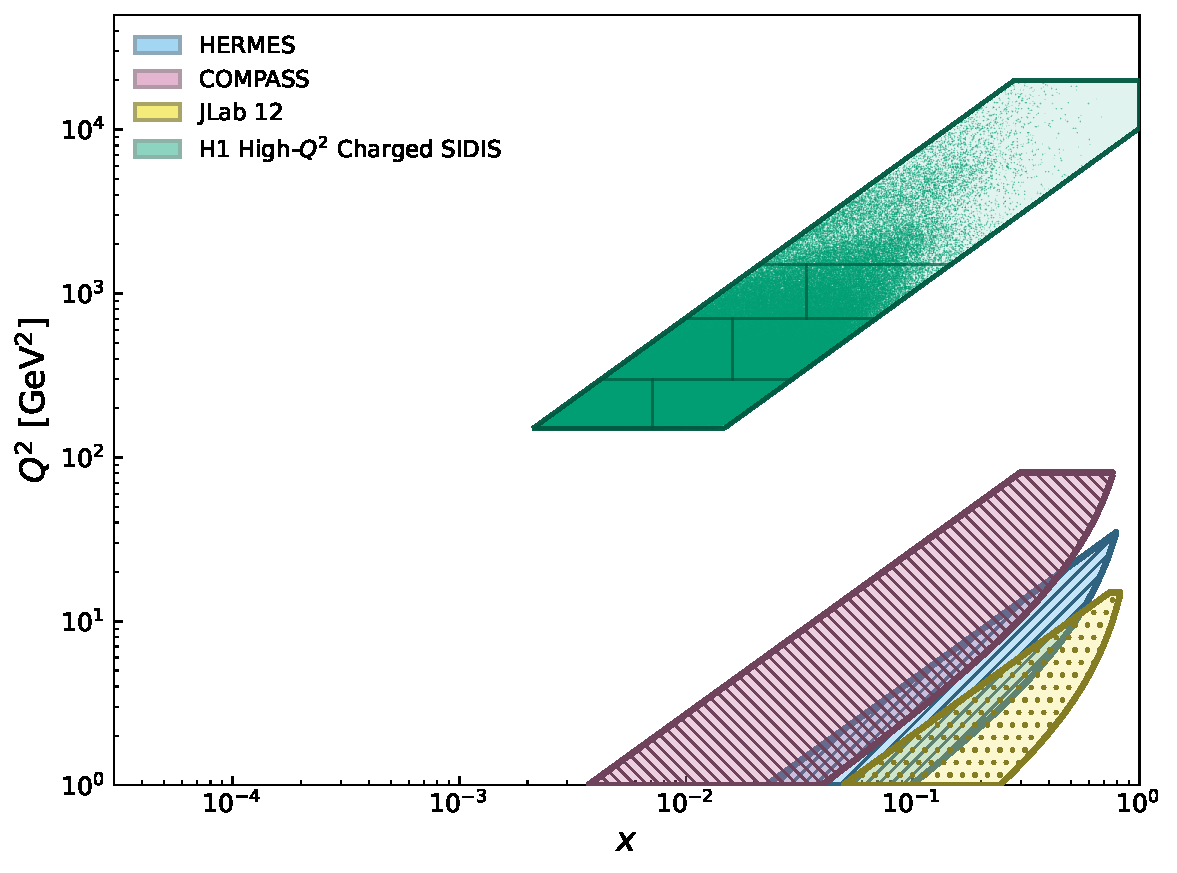
\includegraphics[width=0.82\textwidth]{figures/fig_kinematic_coverage_xQ2_H1.pdf}
\caption{H1 kinematic coverage in the $(x,\Qsq)$ plane.  The high-$\Qsq$
charged-hadron SIDIS measurement documented in this note uses the
$\Qsq>150~\GeVsq$ region and is binned further in $z$, $\pTh$, and charge.}
\label{fig:intro:kinematic-coverage-xq2}
\end{figure}

The radiative correction is applied to all cross sections in this note, which
are therefore Born-level.  A final publication-level review of the correction
is still pending, and the correction is not yet applied at the multiplicity
level.  The measurement is reported at the electron--proton cross-section
level; no virtual-photon--proton conversion is applied or required.

% =============================================================================
%  Section: Experimental Setup
%  H1 Charged-Hadron SIDIS High-Q^2 Analysis Note
% =============================================================================
\section{Experimental Setup}
\label{sec:experimental_setup}

The measurement uses $\ep$ collisions delivered by HERA and recorded with the
H1 detector.  The center-of-mass energy is $\rts=319~\GeV$.  Charged tracks are
reconstructed in the H1 central tracking system. The scattered lepton and the
hadronic final state are reconstructed with the standard H1 high-$\Qsq$ DIS
selection and calibration chain. For more details on the exact algorithms used for high-$Q^2$ analyses, see Refs.~\cite{Kogler:2011zz,Britzger:2013,Peez:2005Hadroo2}

The charged-SIDIS data sample corresponds to an integrated luminosity of
$351~\pbinv$, collected from 2003-2007. This is the luminosity used for the high-$\Qsq$ charged
hadron measurement documented here and for the corresponding low-$\Qsq$ charged
SIDIS analysis.  The luminosity uncertainty included in the high-$\Qsq$ systematic uncertainty budget is a flat $2.7\%$ normalization component.  It is fully
correlated across bins and charges for cross-section-like quantities and cancels
in charge ratios when the same data sample appears in numerator and denominator.

The analysis uses the standard H1 neutral-current DIS event-quality selection,
including the LAr electron acceptance, the S67 high-$\Qsq$ trigger path for data,
and the standard non-ep-background rejection. The exact event selection logic and the
analysis-level fiducial requirements are summarized in Sec.~\ref{sec:selection}.

% =============================================================================
%  Section: Event and Track Selection
%  H1 Charged-Hadron SIDIS High-Q^2 Analysis Note
% =============================================================================
\section{Event and Track Selection}
\label{sec:selection}

The analysis uses the standard H1 high-$\Qsq$ neutral-current DIS event
selection followed by a reconstructed-particle selection for the
charged-hadron measurement.  The event preselection defines the accepted event
sample that is passed to the skimmed analysis TTree and, for simulated samples, keeps additional reconstructed and generator-level
information needed to model detector migrations.  The final analysis selection
is applied identically to the measured reconstructed-particle sample and to the
reconstructed side of the response-matrix construction.

\subsection{DIS Event Preselection}
\label{sec:selection:preselection}

The DIS event preselection requires a well reconstructed scattered-electron
candidate, a good primary vertex, and rejection of non-$ep$ and QED-Compton-like
backgrounds.  The requirements are:
\begin{itemize}
  \item The good-run list and detector-status requirements are applied;
  \item The S67 trigger (electron in the LAr calorimeter) is required;
  \item The scattered-electron energy satisfies $E_e \ge 11.0~\GeV$, and the
        scattered-electron polar angle satisfies $\theta_e < 2.7$ rad;
  \item The event vertex is available from the standard neutral-current vertex
        reconstruction: for forward electrons with $\theta_e<30^\circ$, the CJC
        fallback vertex is also accepted; in either case
        $|z_{\mathrm{vtx}}| \le 35.0~\mathrm{cm}$ is required;
  \item The loose cut envelope used in generation of the skimmed analysis TTree is
        $100 < Q^2_{e\Sigma} \le 20000~\GeVsq$,
        $0.05 < y_{e\Sigma} < 0.9$, $30 < E-p_z < 75~\GeV$, and
        $y_e < 0.94$;
  \item When bunch-type information is available, the colliding-bunch (i.e. not the pilot bunches) category 
        is required.
\end{itemize}

The scattered electron is required to fall in well instrumented regions of the
liquid-argon calorimeter.  The longitudinal impact coordinate must satisfy
\begin{equation}
  -190.0 < z_{\mathrm{impact}} < 15.0
  \quad\mathrm{or}\quad
  z_{\mathrm{impact}} > 25.0,
\end{equation}
and the azimuthal position within a calorimeter octant must avoid the octant
cracks according to
\begin{equation}
  2^\circ < \phi_{\mathrm{octant}} < 43^\circ
  \quad\mathrm{or}\quad
  z_{\mathrm{impact}} > 300.0.
\end{equation}
In addition, a run-dependent electromagnetic-calorimeter fiducial veto is
applied.  The veto is defined by the run number, the electron azimuthal position
at the liquid-argon calorimeter edge, the electron longitudinal impact
coordinate, and the electron energy.  It removes regions where the electron
trigger efficiency is below 100\%.

% Provenance for the non-ep veto fractions quoted here:
% /data/dust/group/h1/klesthen/BaryonAsym/H1ChargedSidis_HighQ2/output_v6/studies/bgfinder_ptratio_cutflow_2026-10-06/merged/summary_bgfinder_cutflow.json
A small fraction of the recorded events do not originate from $ep$ collisions,
but from interactions of the proton beam with residual gas in the beam pipe,
from beam-halo muons, or from cosmic rays traversing the detector.  Such
non-$ep$ backgrounds can mimic DIS events, for example when an unrelated
energy deposit is reconstructed as the scattered electron, but they are
characterised by event times inconsistent with the nominal beam crossing
and by a hadronic system that does not balance the transverse momentum of
the apparent electron candidate.  These events are rejected with the standard H1
timing vetoes: events flagged by the background finders
(flags 0, 1, 5, 6, 7), which combine timing information from the central tracker and the LAr calorimeter with topological information, are removed in
combination with the hadronic-to-electromagnetic transverse-momentum balance
$R=p_T^{\mathrm{had}}/p_T^{e}$.  

A single finder flag is treated as weak
evidence, since the finders occasionally also flag genuine $ep$ events, and
leads to rejection only when corroborated by a significant momentum
imbalance, $R<0.1$ for finder 7 and $R<0.5$ for finders 5 or 6, whereas two
simultaneous finder flags are treated as sufficient evidence and lead to
rejection for events with $R>0.1$.  The veto rejects 0.29\% of the events
passing all preceding selection requirements, while 1.61\% of these events
have $R<0.5$ (0.06\% have $R<0.1$) and are retained in the absence of a
corroborating finder flag, so the timing and kinematic criteria act jointly
rather than as independent requirements.  The anti-QED-
Compton veto rejects events with two electromagnetic particles when the two
leading electron candidates each have energy above $4~\GeV$, their summed energy
is above $18~\GeV$, and the two candidates are nearly back-to-back in azimuth,
$-\cos(|\phi_1-\phi_2|)>0.95$.

\subsection{Final Reconstructed-Event Selection}
\label{sec:selection:final-events}

The final reconstructed-event selection tightens the DIS phase space used for
the measurement:
\begin{itemize}
  \item $150 < Q^2 < 20000~\GeVsq$;
  \item $0.1 < y < 0.7$;
  \item $E-p_z > 45~\GeV$;
  \item $|z_{\mathrm{vtx}}| < 35~\mathrm{cm}$;
\end{itemize}
The same reconstructed-event requirements are used for the response-matrix
construction and for the measured event sample.

\subsection{Final Reconstructed-Track Selection}
\label{sec:selection:final-tracks}

The measured charged-hadron sample consists of reconstructed charged tracks
passing the track-quality, topology, and analysis-bin requirements.  Accepted tracks are counted only as inclusive $\hplus$ or $\hminus$ candidates according to the sign of their electric charge.
The truth-level charged-hadron convention used for acceptance and migration
modeling is documented in Sec.~\ref{sec:species_definition}.

The final reconstructed-track cuts are:
\begin{itemize}
  \item Lab-frame transverse momentum $p_T>0.15~\GeV$ and pseudorapidity $|\eta|<1.6$;
  \item At least 5 hits in the CJC
  \item Radial track length at least 5 cm;
  \item $|\mathrm{DCA}'|\sin\theta < 2$ cm,
  \item The track is labeled as originating from the primary vertex in H1OO;
  \item The reconstructed track is in the current hemisphere, i.e. $x_F<0$ in the H1 convention;
  \item The reconstructed $z$ and $\gamma^*p$-frame $\pTh$ are finite and inside
        the analysis binning.
   \item The opening angle between the track and the scattered electron is more than 0.2 radians.
\end{itemize}
The analysis binning uses
$z=[0.0,0.05,0.1,0.2,0.3,0.5,0.7,1.0]$ and reconstructed
$\pTh=[0.0,0.25,0.5,0.75,1.0,1.5,2.0,3.0,4.0,6.0,8.0]~\GeV$ edges.  The first
physical $z$ bin is $0.0 \le z < 0.05$.

A reconstructed-side opening-angle requirement suppresses tracks close to the
scattered-electron direction, which can come from final-state radiated photon conversions or mis-identification of the scattered electron track.  For each reconstructed track, the opening angle
to the scattered-electron three-vector, $\alpha$, is calculated in the lab frame. Accepted tracks must satisfy
$\alpha(\mathrm{track},e') \ge 0.2~\mathrm{rad}$.  This requirement is applied
only to reconstructed tracks; the corresponding generator-level loss of true charged hadrons is 0.106\% for RAPGAP and 0.114\% for DJANGOH.

% =============================================================================
%  Section: Monte Carlo Simulation
%  H1 Charged-Hadron SIDIS High-Q^2 Analysis Note
% =============================================================================
\section{Monte Carlo Simulation}
\label{sec:monte_carlo}

The detector corrections are derived from fully simulated H1 Monte Carlo
samples processed with the same charged-SIDIS reconstruction chain as the
data.  The nominal signal-model comparison uses DJANGOH and RAPGAP response
matrices.  DJANGOH provides a DIS sample with QED radiative effects through
HERACLES and QCD shower modelling through the standard H1 generator chain;
RAPGAP provides an independent DIS generator model for the response and model
uncertainty comparison \cite{Charchula:1994kf,Kwiatkowski:1990es,Jung:1993gf}.
Detector simulation uses the standard H1 GEANT-based chain \cite{Brun:1987ma}.

MC event weights are applied consistently in the response and data-vector
construction.  The standard factors are the generator weight, the L5 user
weight, the trigger weight where applicable, and the nuclear interaction cross section correction weight.

The response builder does not impose final generator-level fiducial cuts such as
GenPt, GenEta, $x_F$, final-$\Qsq$, $y$, or $E-p_z$ inside the migration-matrix
construction.  It applies the finite-$z_{\mathrm{gen}}$ filter and the charged
hadron species/source/V0-veto conventions, while the final physics fiducial is
imposed at the unfolding and truth-selection stage.  This separation keeps the
migration matrix reusable for the nominal release and for systematic variants.

\subsection{Generators Used in the Cross-Section Comparison}
\label{sec:monte_carlo:comparison-generators}

The diagnostic data--MC comparison of
Sec.~\ref{sec:results:diagnostic-4d-cross-sections} overlays four generator
predictions on the Born-level unfolded data: the two H1 detector-MC generators
DJANGOH14 and RAPGAP31, and the two standalone generator-level programs
PYTHIA~8.317 and SHERPA~3.0.3.

DJANGOH14 \cite{Charchula:1994kf} is the H1 detector-MC signal generator.  QED
radiation from the lepton line is generated through HERACLES
\cite{Kwiatkowski:1990es}, the hard DIS scattering through LEPTO
\cite{Ingelman:1996mq}, and the QCD cascade through the ARIADNE colour-dipole
model \cite{Lonnblad:1992tz}, using the CTEQ6L parton distribution functions.
The RAD high-$\Qsq$ (Q2GT60) samples are passed through the full GEANT-based H1
detector simulation \cite{Brun:1987ma} and the same reconstruction chain as the
data.  They cover the four HERA-II periods with ReqIDs 7093 (ep0304), 7092
(em0405), 7072 (em06), and 7091 (ep0607), with a combined MC luminosity of
$10{,}487{,}495.0~\nbinv$.  DJANGOH14 is also the source of the applied per-bin
$C_{\mathrm{rad}}$ primary used for the Born-level conversion.

RAPGAP31 \cite{Jung:1993gf} is an independent DIS generator combining
order-$\alpha_s$ matrix elements with a leading-logarithm parton shower, also
using CTEQ6L.  QED radiation through HERACLES is included in its RAD sample,
again for the high-$\Qsq$ (Q2GT60) selection.  Its four HERA-II periods carry
ReqIDs 7097 (ep0304), 7096 (em0405), 7071 (em06), and 7094 (ep0607), with a
combined MC luminosity of $9{,}132{,}891.0~\nbinv$.  RAPGAP31 provides the
central unfolding response of the current release.

PYTHIA~8.317 \cite{Sjostrand:2014zea} and SHERPA~3.0.3 \cite{Sherpa:2019gpd}
provide standalone generator-level predictions without detector simulation.
Both are generated rad-off, with no QED radiation from the lepton line.  The
PYTHIA8 setup uses the dipole shower with Lund string fragmentation and the
audit-fixed DIS steering \texttt{SpaceShower:dipoleRecoil=on},
\texttt{SpaceShower:pTmaxMatch=2}, \texttt{PDF:lepton=off}, with the
lepton-line QED shower switched off.  The SHERPA3 setup uses Comix Born
leading-order DIS matrix elements with AHADIC cluster hadronization and the
\texttt{NNPDF31\_lo} parton distribution functions \cite{Ball:2017nwa}, with
the YFS and \texttt{ME\_QED} QED stages disabled.  Each program was produced
as a Rivet sample of $10^{7}$ generated events.

The particle-level truth definition in the generators is the same as the analysis convention: final-state $\pi^{\pm}$, $K^{\pm}$, $p$, and $\bar p$ with
$|\mathrm{PDG}|\in\{211,321,2212\}$ and no ancestor among the long-lived
states $\{310,130,3122,3222,3112,3312,3322,3334\}$. Decay daughters of
short-lived resonances and heavy flavors are retained. 

Because PYTHIA8 and SHERPA3 are rad-off, their predictions are compared
directly with the Born-level data.  The RAPGAP31 and DJANGOH14 truth curves
are the generators' non-radiative (NORAD) sample predictions. Thus all four
overlaid curves sit at the non-radiative level of the Born-corrected data.

% =============================================================================
%  Section: Observables
%  H1 Charged-Hadron SIDIS High-Q^2 Analysis Note
% =============================================================================
\section{Observables}
\label{sec:observables}

The primary high-$\Qsq$ charged-SIDIS observables are charge-separated cross sections binned in $(\Qsq,x,z,\pTh)$. We define the differential SIDIS cross section using the unfolded yields ($N_{\mathrm{Unf.}}$), the integrated luminosity ($\mathcal{L}=351$ pb$^{-1}$), the 4D bin volume ($\Delta x\Delta Q^2\Delta z \Delta p_{T,h}$) and the radiative correction factor ($c_{\mathrm{rad}}$):

\begin{equation}
    \frac{d\sigma}{dxdQ^2dzdp_{T,h}} = \frac{N_{\mathrm{Unf.}}\times c_{\mathrm{rad}}}{\mathcal{L}\times\Delta x\Delta Q^2\Delta z \Delta p_{T,h}}.
\end{equation}


The azimuthal variables $\phih$ and the moments
$\langle\cos\phih\rangle$ and $\langle\cos2\phih\rangle$ are defined in the
$\gamma^{*}p$ center-of-mass frame.  Earlier lab-frame diagnostic columns are
not used for the current release.

% =============================================================================
%  Section: Hadron Species Definition
%  H1 Charged-Hadron SIDIS High-Q^2 Analysis Note
% =============================================================================
\section{Hadron Species Definition}
\label{sec:species_definition}

The measured analysis is inclusive in charged hadrons and does not separate
pions, kaons, and protons with particle identification.  At reconstruction level
all selected charged tracks enter either the $\hplus$ or $\hminus$ sample,
subject to the standard charged-SIDIS track-quality and veto requirements.

The truth-level convention used for generator denominators, response matrices,
and matching pools is restricted to charged pions, charged kaons, and protons:
\begin{equation}
  |\mathrm{PDG}| \in \{211,\;321,\;2212\}\, .
\end{equation}
This convention is shared by the low- and high-$\Qsq$ charged-SIDIS analyses.
It excludes hyperons and other charged particles from the truth denominator,
and it defines the hadron content of the inclusive $\hpm$ measurement for
acceptance and migration purposes.  No additional PID correction is applied to
split the final result by species.

% =============================================================================
%  Section: Reconstructed-Track Backgrounds
%  H1 Charged-Hadron SIDIS High-Q^2 Analysis Note
% =============================================================================
\section{Backgrounds}
\label{sec:backgrounds}

The only event-level background arises from DIS events outside the measurement phase space which migrate in due to resolution effects or QED radiation. The phase space of $60 < Q^2< 150$ GeV$^2$ is handled by the high $Q^2$ DJANGOH and RAPGAP MC samples. The region $Q^2 < 60$ GeV$^2$ is handled by a dedicated Djangoh sample, which has negligible contribution in almost all bins. The distributions of this low $Q^2$ background are shown in Fig.~\ref{fig:bg:alpha0p2-reco-background-fractions}. The background from $Q^2 < 4$ GeV$^2$ (including photoproduction) was evaluated with Pythia and found to be negligible, only 5 photoproduction events are expected in the whole event sample. Similarly, the contribution from exclusive vector meson production was studied with DIFFVM elastic $\rho$ production.  Its integrated contribution is negligible, $0.0074\%$ of the reconstructed-track denominator, but it is bin-localized at high $z$: the $z$ row $0.7\le z<1.0$ reaches $2.18\%$ and the worst single cell $4.53\%$.  The measured elastic-$\rho$ contribution is reserved as a systematic-only, source-distinct template; it is not subtracted per bin and is not part of the current systematic budget.  The $\phi$ and $\omega$ channels and proton-dissociative $\rho$ production remain unquantified caveats.  For this analysis, diffractive DIS is not subtracted.

After the charged-SIDIS event and track
selection, two non-negligible reconstructed-track background categories are
considered in the current high-$\Qsq$ analysis:
\begin{enumerate}
  \item electron and positron tracks, including tracks from Dalitz decays or
        semi-leptonic decays of mesons;
  \item charged tracks arising from decays of long-lived neutral hadrons.
\end{enumerate}


The electron background category is modeled by selecting reconstructed electrons or positrons in DJANGOH and RAPGAP. This background arises from photon conversions, hadron decays, or tracks from scattered electrons or positrons which are not properly matched to their calorimeter cluster. The mis-identified scattered-electron background is reduced by rejecting tracks within $0.2$ radians of the nominal scattered-electron three-vector, which can come from the calorimeter cluster; accepted tracks satisfy
$\alpha(\mathrm{track},e')\ge0.2~\mathrm{rad}$. The remaining $e^\pm$ background arises mainly from meson decays and lives mostly at low-$z$.
Since the cone-baseline promotion of 2026-10-13 this requirement is part of
the central selection rather than a diagnostic variant; cone-rejected matched
legs flow to the miss row of the response.

The V0 decay daughter category is identified through the absolute value of
a multi-hop search for a V0 PDG code.  The exact ancestor set used is
\begin{equation}
  |\mathrm{PDG}_{\mathrm{ancestor}}| \in \{310,\;130,\;311,\;3122\}\, ,
\end{equation}
corresponding to $K^{0}_{S}$, $K^{0}_{L}$, $K^{0}/\bar K^{0}$, and
$\Lambda/\bar\Lambda$ ancestors.  This is the definition used to remove background from V0s.

In the current response, the detector-interaction removable
class is removed response-internally through an enlarged per-reco-bin fake
fraction $f_i$ (pooled removable fraction $0.9096$), while charged kaons
from detector interactions with a reconstructed parent are kept as signal.  An
external subtraction of the detector-interaction component is therefore
forbidden: it would double-remove the class.  Electrons and V0 daughters are
in addition vetoed at the selection level, and their residual contamination,
together with the low-$\Qsq$ leakage, is subtracted from the data vector
before unfolding using the Monte Carlo background templates; the total
subtracted content is $281{,}250.09$ tracks, $7.2767\%$ of the cone data
vector.

The current canonical reco-background fraction display is shown in
Fig.~\ref{fig:bg:alpha0p2-reco-background-fractions}.  The fraction is defined
as the expected background-track count divided by the reconstructed-track
count after the $\alpha<0.2$ selection in the same
$(\Qsq,x,z,\pTh,\mathrm{charge})$ bin. The plotted
components are the residual $e^\pm$ background, the matched-V0-daughter
background, the low-$\Qsq$ component, and their total where shown. The integrated reco track count is $3{,}865{,}073$, of which the estimated track-level background total at $\mathcal{L}=351000.0~\nbinv$ is $308{,}655.9$ ($7.986\%$), split into $148{,}976.4$ electron and positron tracks, $132{,}065.3$ V0 decay daughters, $27{,}405.8$ detector-interaction secondaries, and $208.4$ low-$\Qsq$ leakage tracks, with the $e^\pm$ and V0 components located mostly at low $z$.
Of these four categories, the electron, V0, and low-$\Qsq$ components are the
ones subtracted from the data vector before unfolding in the current release;
the detector-interaction component is not subtracted externally but removed
response-internally, as described above.

The curves for the $e^\pm$ and V0 backgrounds are taken as the average of DJANGOH and RAPGAP.

\begin{figure}[p]
  \centering
  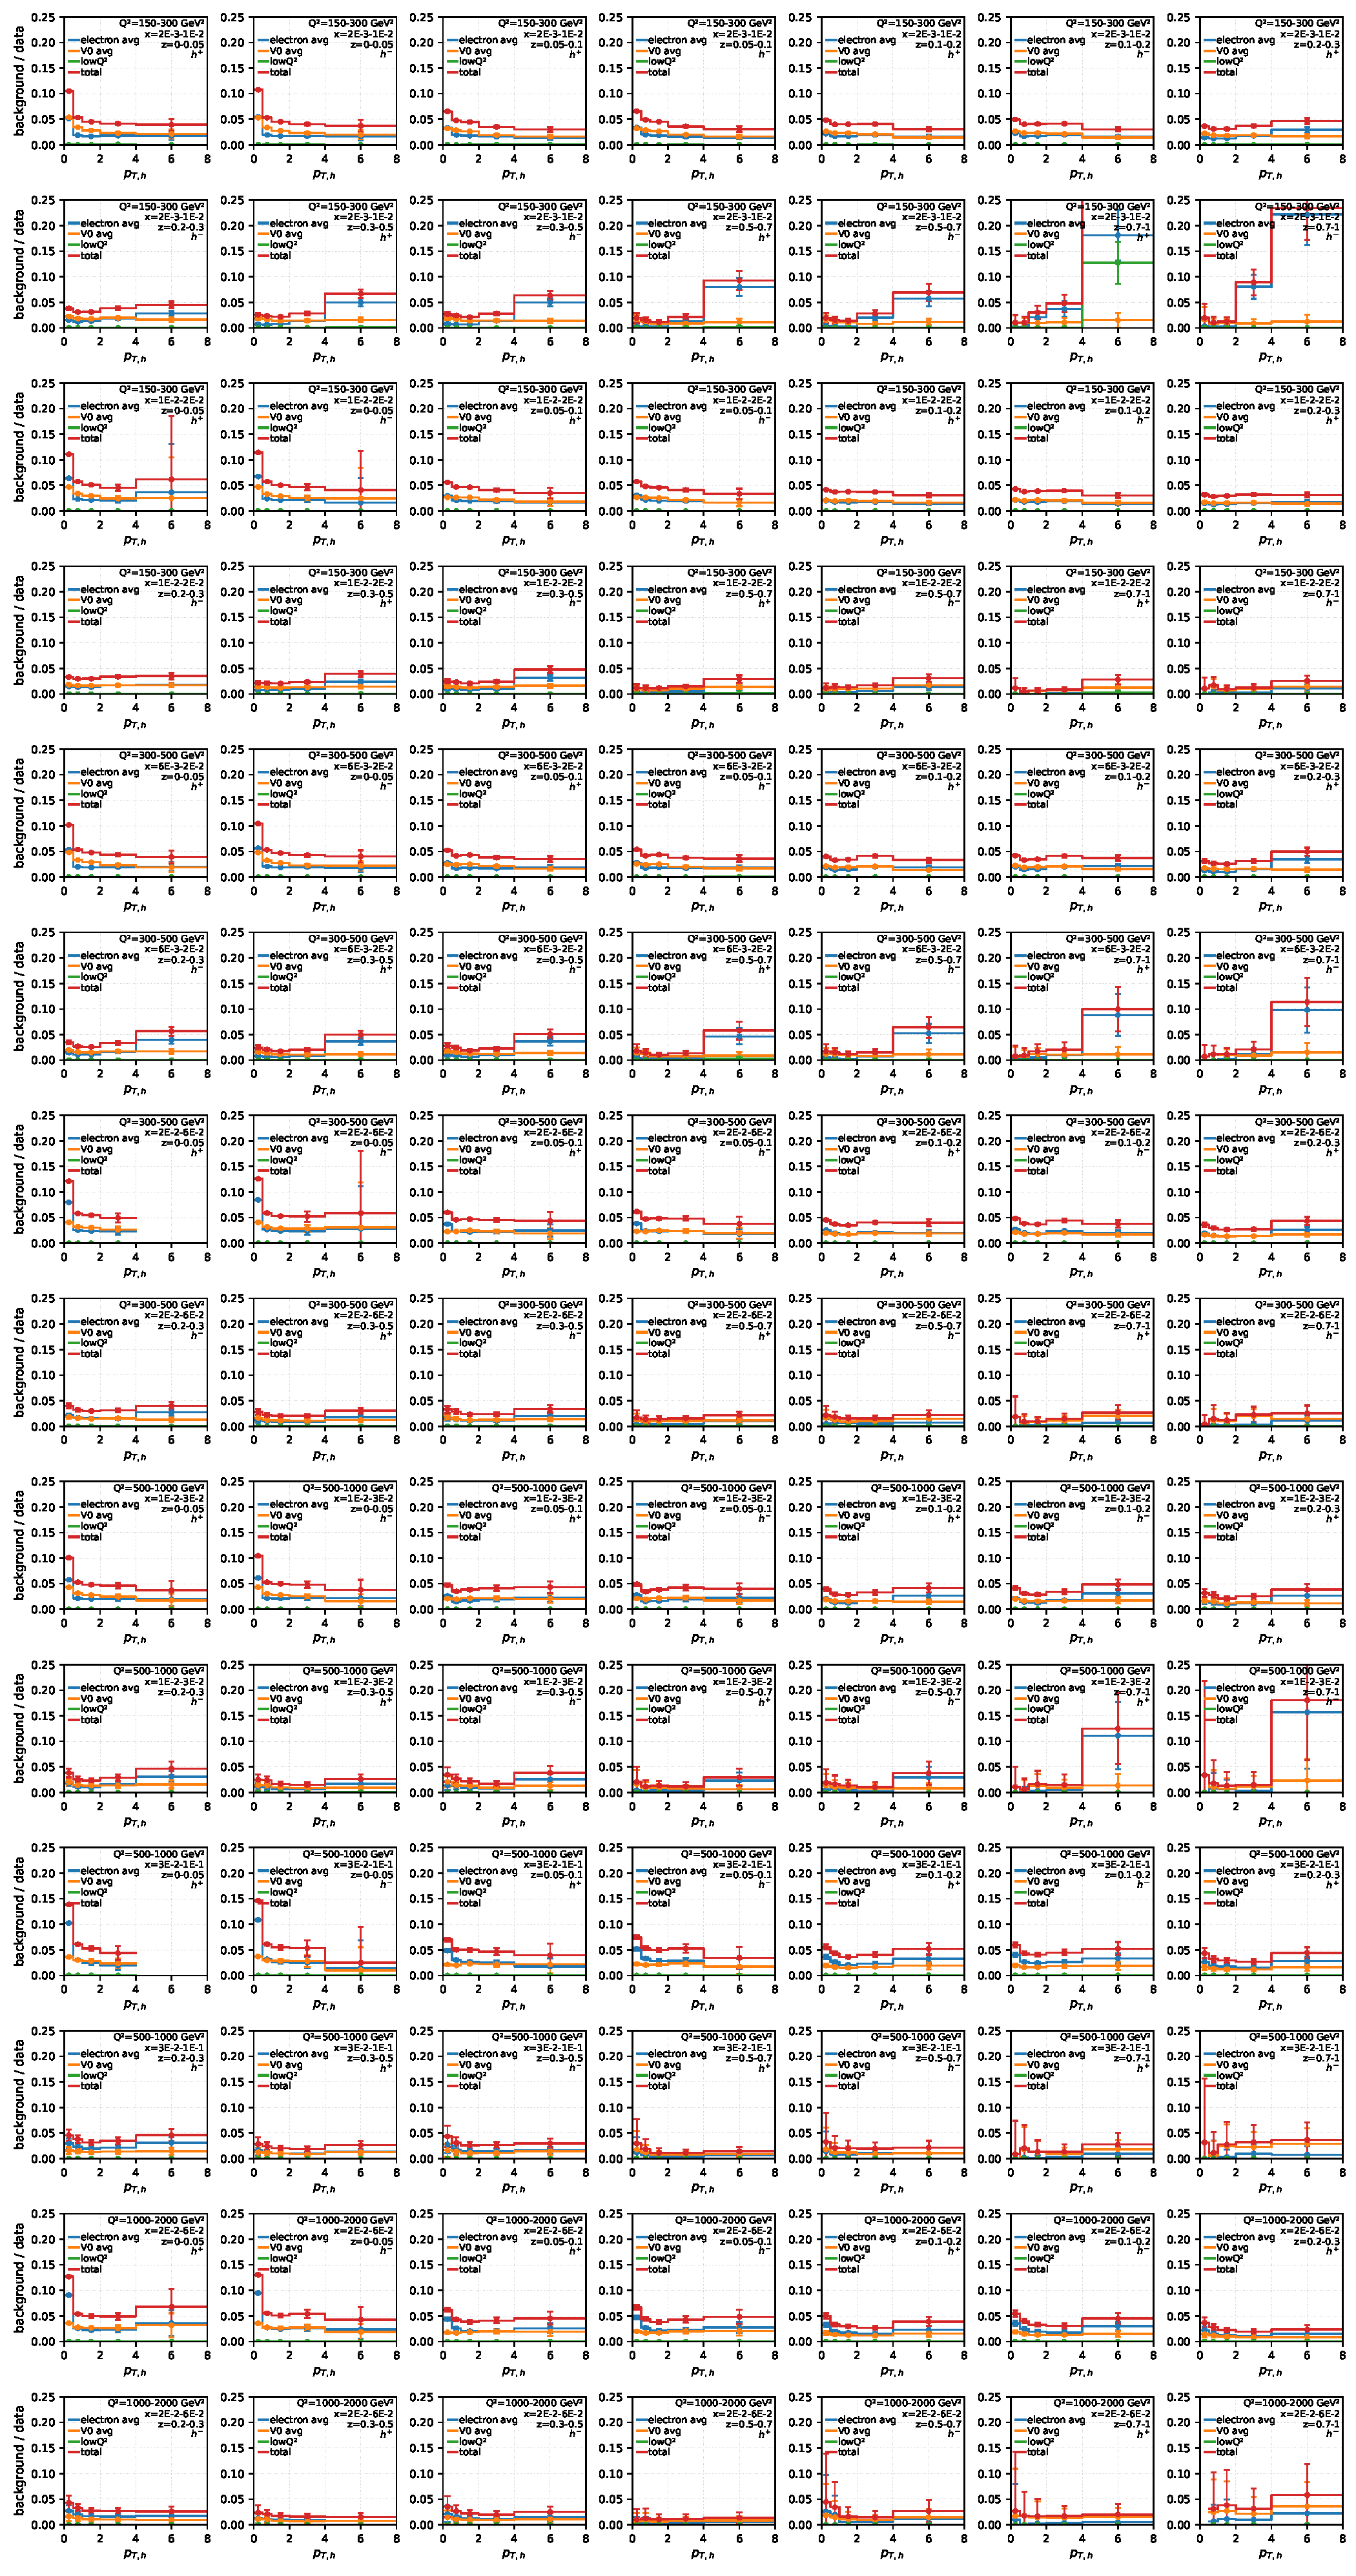
\includegraphics[width=0.95\textwidth,height=0.9\textheight,keepaspectratio]{figures/fig_reco_background_fractions_alpha0p2_onepage_7col.pdf}
  \caption{Reco-level background fractions after the $\alpha<0.2$ selection,
  defined as the number of background tracks divided by the number of reco tracks in the same
  $(\Qsq,x,z,\pTh,\mathrm{charge})$ bins.  The
  first column corresponds to $0.0 \le z < 0.05$.}
  \label{fig:bg:alpha0p2-reco-background-fractions}
\end{figure}

As a complementary diagnostic display of the background model,
Figs.~\ref{fig:bg:reco-multiplicity-dist-per-cell}
and~\ref{fig:bg:reco-multiplicity-dist-combined} show the raw, uncorrected
per-event multiplicity distributions of reconstructed charged hadrons in the
seven $(\Qsq,x)$ cells of Table~\ref{tab:binning:z005-contract}, with the
per-source background expectations overlaid.  The event sample is the
analysis-fiducial selection of Sec.~\ref{sec:selection:final-events}:
$0.1<y_{e\Sigma}<0.7$, $E-p_z>45~\GeV$, $150<\Qsq<20000~\GeVsq$, and
$|z_{\mathrm{vtx}}|<35~\mathrm{cm}$.  The overlaid expectations are expected
event counts at $\mathcal{L}=351000.0~\nbinv$ ($351~\pbinv$) from the
alpha0p2 background chain, shown separately for four sources: electron
tracks, V0 decay daughters, detector-interaction secondaries, and
low-$\Qsq$ leakage (fid-gate overlay variant).  Each background curve is
displayed as expected events versus the number of that source's background
tracks per event; its $n=0$ entry is the fiducial event population
containing none of that source.  The background model is
diagnostic/provisional and is not a physics-approved subtraction.  The
figures, their input tables, and the $n=0$ convention are documented in the
figure package \path{sidis_highQ2/plots/reco_multiplicity_note_2026-10-07/}
(README.txt); the data input tables are the v6 fid-variant study outputs
\path{H1ChargedSidis_HighQ2/output_v6/studies/reco_multiplicity_dist_2026-10-07/}
and
\path{H1ChargedSidis_HighQ2/output_v6/studies/reco_multiplicity_dist_combined_2026-10-08/},
and the background input table is
\path{H1ChargedSidis_HighQ2/output_v6/studies/reco_backgrounds_multdist_2026-10-07/aggregate/background_multdist_per_cell_L351000.csv}.

\begin{figure}[p]
  \centering
  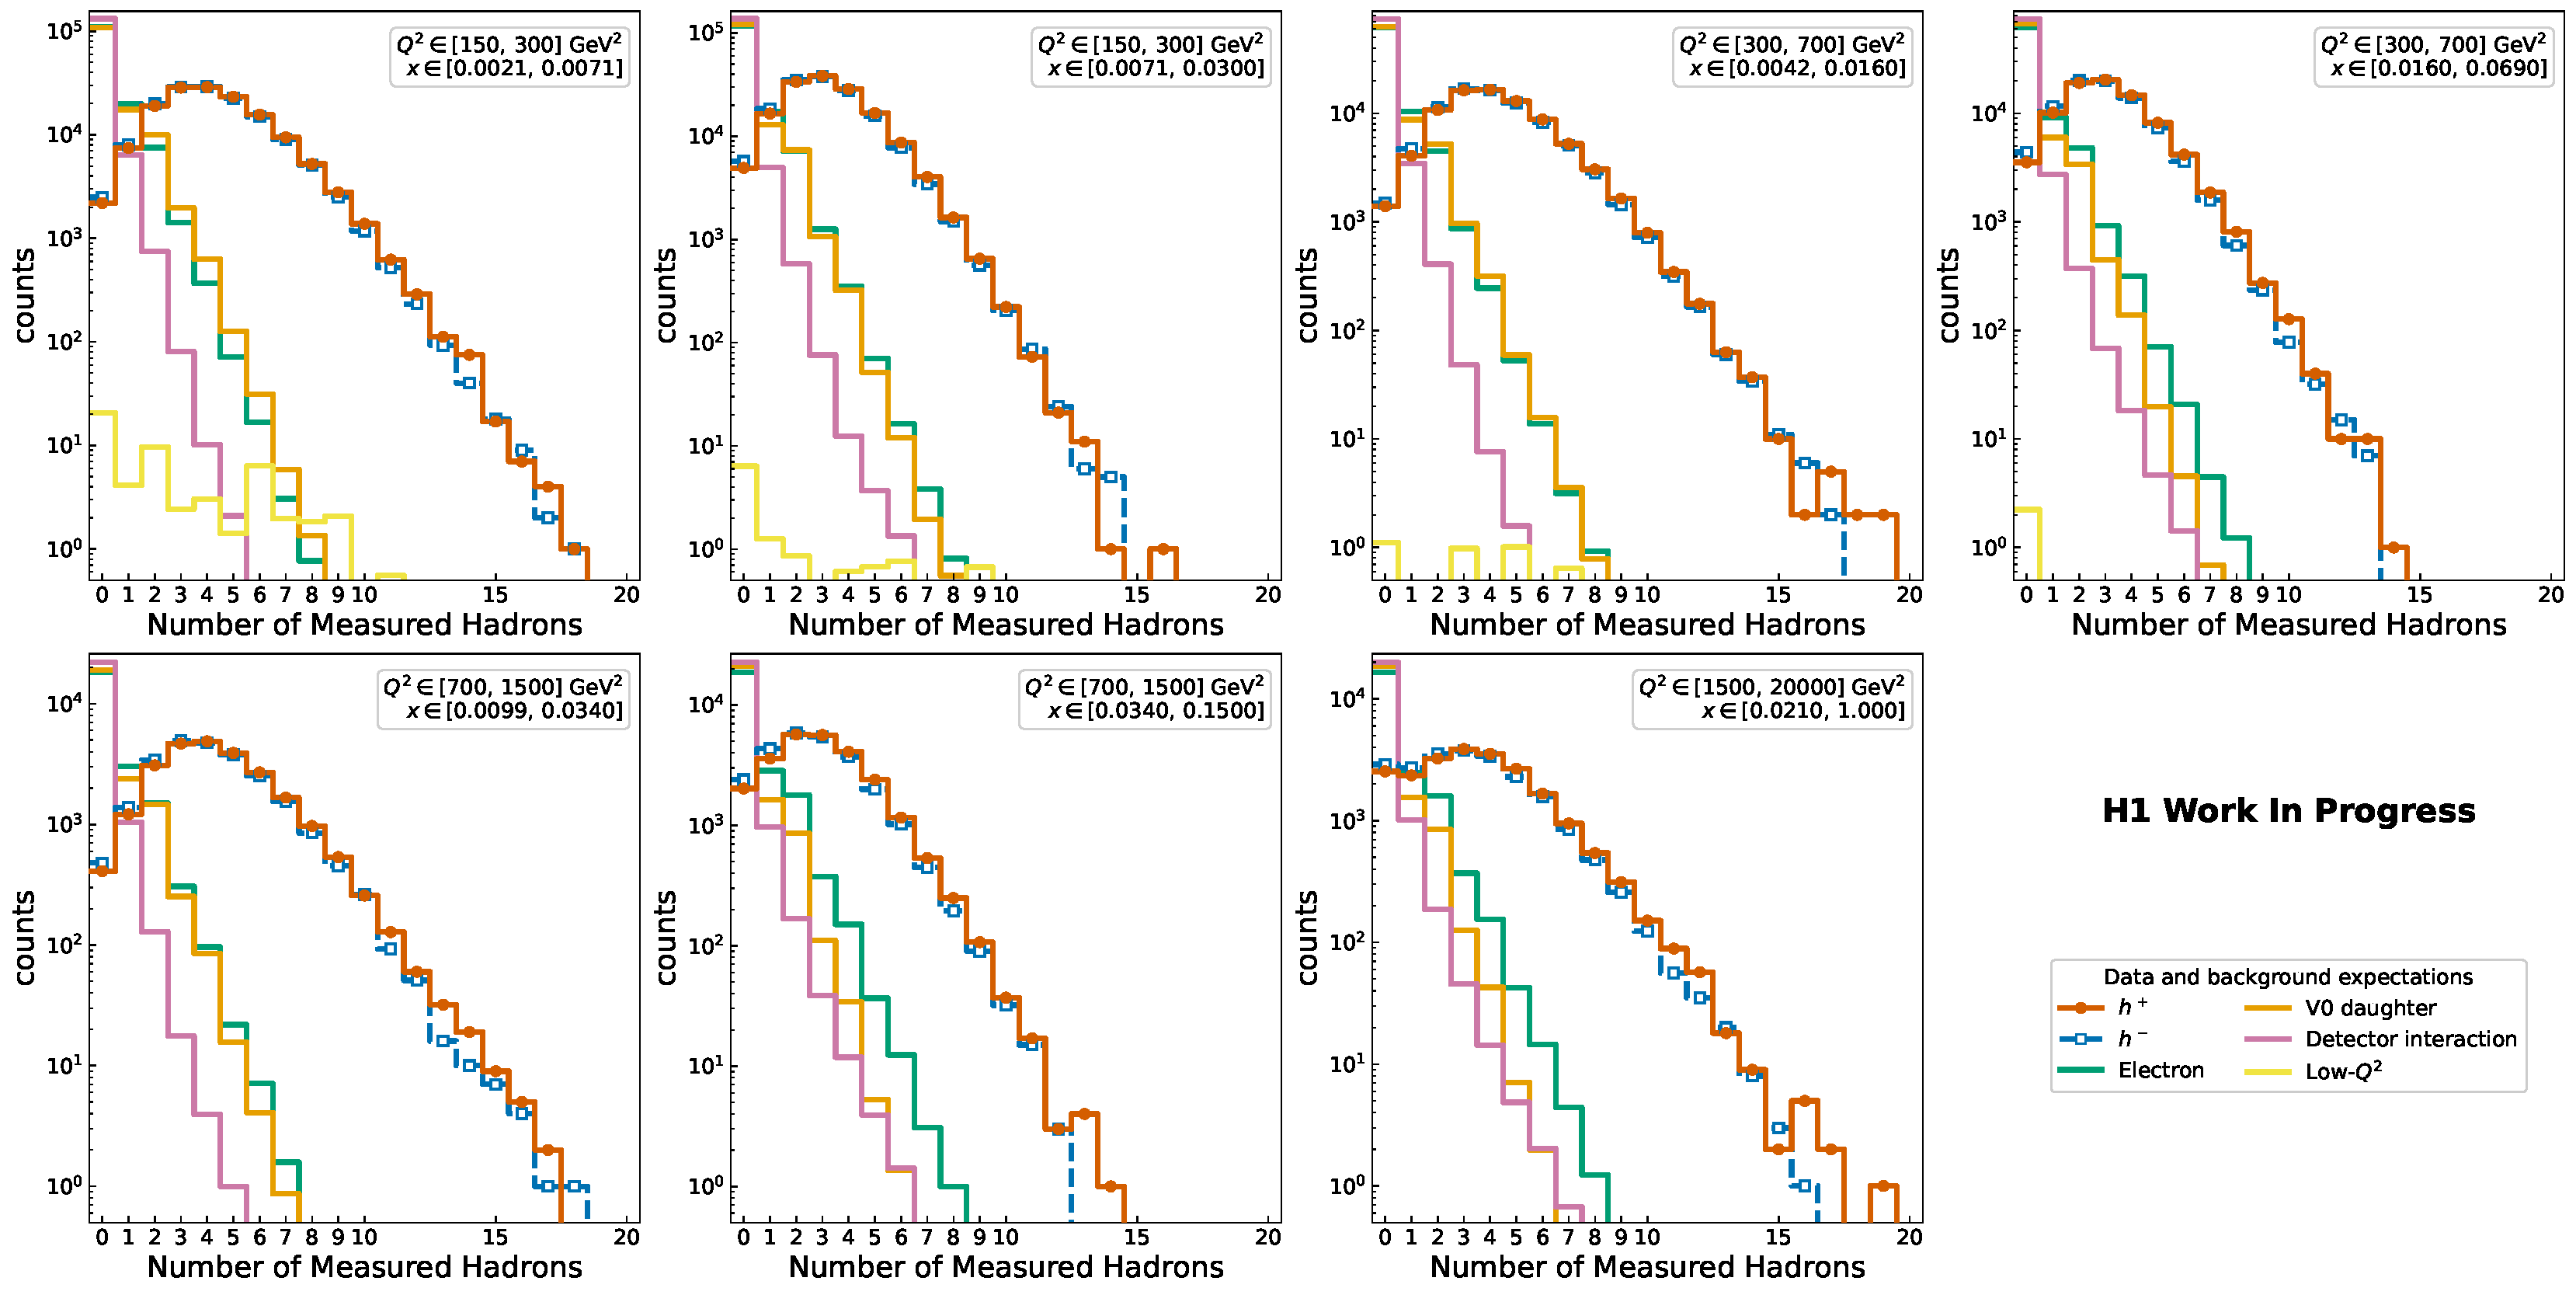
\includegraphics[width=0.98\textwidth,height=0.82\textheight,keepaspectratio]{figures/fig_reco_multiplicity_dist_per_cell_hQ2_v6data_20261007.pdf}
  \caption{Raw, uncorrected per-event multiplicity distributions of
  reconstructed charged hadrons in the seven $(\Qsq,x)$ cells for the
  analysis-fiducial event selection ($0.1<y_{e\Sigma}<0.7$,
  $E-p_z>45~\GeV$, $150<\Qsq<20000~\GeVsq$,
  $|z_{\mathrm{vtx}}|<35~\mathrm{cm}$), shown on a logarithmic y-axis.
  $\hplus$ (filled circles) and $\hminus$ (open squares) are shown
  separately in each cell.  Overlaid are the background expectations at
  $\mathcal{L}=351000.0~\nbinv$ ($351~\pbinv$) from the alpha0p2 background
  chain -- electron, V0 daughter, detector-interaction secondaries, and
  low-$\Qsq$ leakage (fid-gate overlay variant) -- each as expected events
  versus the number of that source's background tracks per event; the $n=0$
  entry of each background curve is the fiducial event population containing
  none of that source.  The background model is diagnostic/provisional.}
  \label{fig:bg:reco-multiplicity-dist-per-cell}
\end{figure}

\begin{figure}[p]
  \centering
  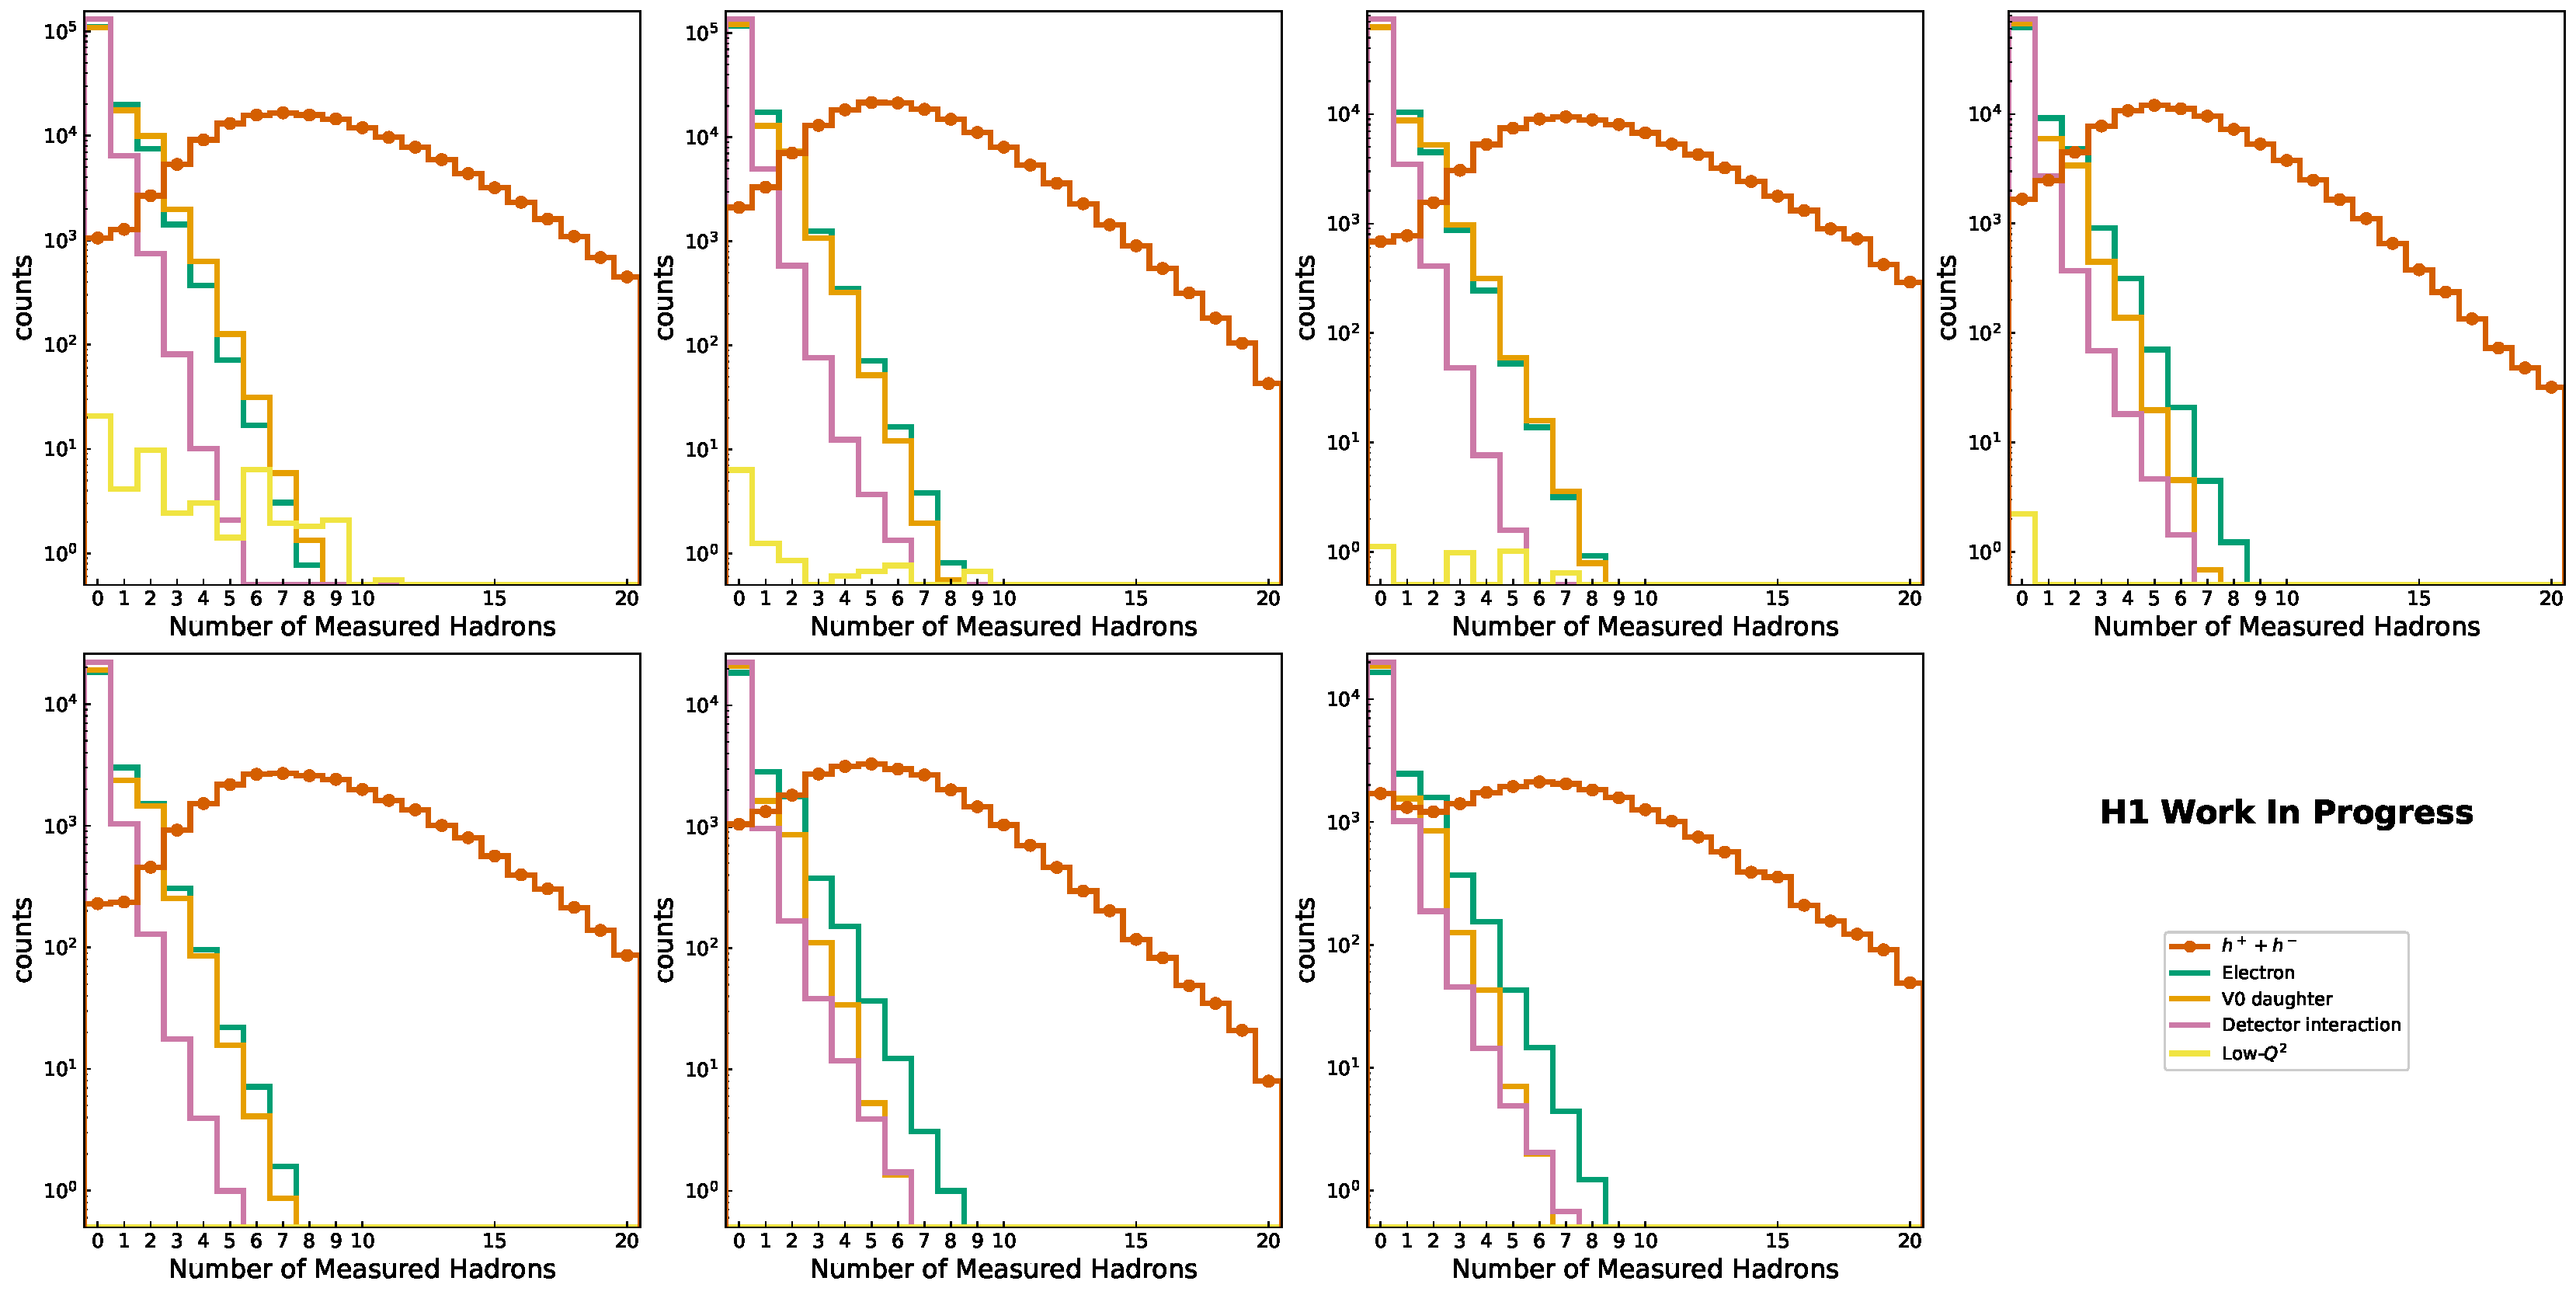
\includegraphics[width=0.98\textwidth,height=0.82\textheight,keepaspectratio]{figures/fig_reco_multiplicity_dist_per_cell_combined_hQ2_v6data_20261008.pdf}
  \caption{Raw, uncorrected per-event total charged-hadron multiplicity
  $n_{\hplus}+n_{\hminus}$ in the seven $(\Qsq,x)$ cells for the
  analysis-fiducial event selection ($0.1<y_{e\Sigma}<0.7$,
  $E-p_z>45~\GeV$, $150<\Qsq<20000~\GeVsq$,
  $|z_{\mathrm{vtx}}|<35~\mathrm{cm}$), shown on a logarithmic counts axis;
  each event is counted once at its total $n_{\hplus}+n_{\hminus}$.  Events
  with $n\ge21$ are excluded from the $0$--$20$ axis; the excluded event
  counts are S0\_x0: 818, S1\_x0: 520, S2\_x0: 213, S3\_x0: 144,
  S0\_x1: 60, S1\_x1: 35, and S2\_x1: 14.  Overlaid are the
  background expectations at $\mathcal{L}=351000.0~\nbinv$
  ($351~\pbinv$) from the alpha0p2 background chain -- electron, V0
  daughter, detector-interaction secondaries, and low-$\Qsq$ leakage
  (fid-gate overlay variant) -- each as expected events versus the number of
  that source's background tracks per event; the $n=0$ entry of each
  background curve is the fiducial event population containing none of that
  source.  The background model is diagnostic/provisional.}
  \label{fig:bg:reco-multiplicity-dist-combined}
\end{figure}

% =============================================================================
%  Section: Kinematic Binning
%  H1 Charged-Hadron SIDIS High-Q^2 Analysis Note
% =============================================================================
\section{Kinematic Binning}
\label{sec:binning}

The current high-$\Qsq$ analysis uses the binning summarized in Table~\ref{tab:binning:z005-contract}.  The
corresponding inclusive DIS measurement phase space in the $(x_{\mathrm{Bj}},
\Qsq)$ plane is shown in Fig.~\ref{fig:binning:kinematic-plane}.  The published
$\pTh$ bins are coarser than the reconstruction-level $\pTh$ bins used in the
response matrix.

\begin{figure}[t]
\centering
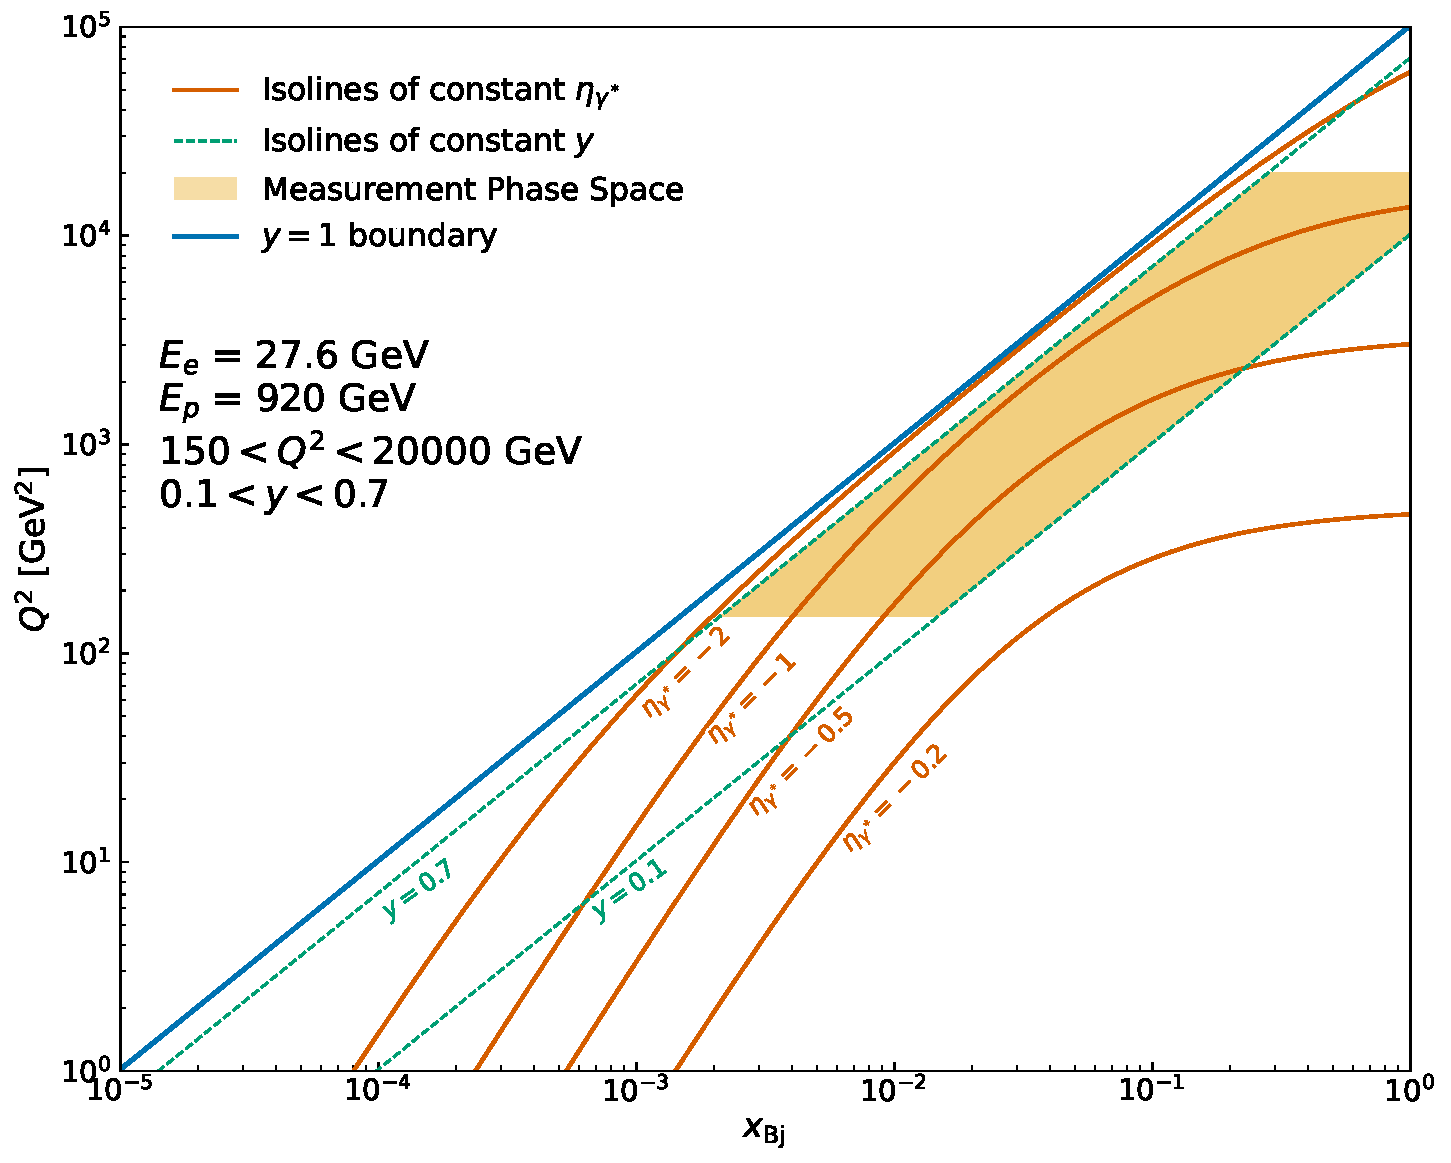
\includegraphics[width=0.82\textwidth]{figures/HERA_xQ2_virtual_photon_eta.pdf}
\caption{Measurement phase space in the $(x_{\mathrm{Bj}},\Qsq)$ plane for the
high-$\Qsq$ charged-hadron SIDIS analysis.  The shaded region indicates the
measurement phase space, and the orange curves show isolines of constant
$\eta_{\gamma^{*}}$ for the virtual photon.  Constant-$y$ isolines and the
$y=1$ boundary are shown for orientation.}
\label{fig:binning:kinematic-plane}
\end{figure}

\begin{table}[h]
\centering
\small
\begin{tabular}{lp{9.3cm}}
\toprule
Quantity & Contract \\
\midrule
$z$ edges (7 bins) & $[0.0,0.05,0.1,0.2,0.3,0.5,0.7,1.0]$ \\
Published $\pTh$ edges (5 bins) & $[0.0,0.5,1.0,2.0,4.0,8.0]~\GeV$ \\
$(\Qsq,x)$ intervals (7 cells) & $150<\Qsq<300~\GeVsq$: $0.0021<x<0.0071$ and $0.0071<x<0.030$; $300<\Qsq<700~\GeVsq$: $0.0042<x<0.016$ and $0.016<x<0.069$; $700<\Qsq<1500~\GeVsq$: $0.0099<x<0.034$ and $0.034<x<0.150$; $1500<\Qsq<20000~\GeVsq$: $0.021<x<1.0$\footnotemark \\
Published bins & 245 per charge; 490 total \\
Response and data vectors & Response matrix $(491,246)$ per charge; data-vector length 980 \\
\bottomrule
\end{tabular}
\caption{Validated binning and response contract for the current high-$\Qsq$
analysis release.  The reconstruction-level $\pTh$ binning is deliberately
finer than the published binning.}
\label{tab:binning:z005-contract}
\end{table}
\footnotetext{The internal binning container carries $x_{\max}=1.5$ only to catch migrations; it is not part of the published binning.}

The binning is charge separated: every published bin appears once for $\hplus$
and once for $\hminus$.  The generator-side published grid contains 245 bins per
charge.  

The reconstructed-side binning used in the migration matrix is twice as fine in $\pTh$, using the ten-bin edge set given in Sec.~\ref{sec:selection:final-tracks}, with 490 reconstructed bins total per
charge.  This permits migrations to be modeled before the result is unfolded
back to the 245-bin published grid per charge. An additional row and column in
the stored migration matrix is used for handling fakes and misses.


%% =============================================================================
%  Section: Acceptance Corrections
%  H1 Charged-Hadron SIDIS High-Q^2 Analysis Note
% =============================================================================
\section{Acceptance Corrections}
\label{sec:acceptance}

Detector acceptance and bin migration are treated together through the response
matrices used by the unfolding.  The z005 release stores both bin-by-bin (BBB)
and iterative Bayesian unfolding (IBU) products.  The BBB correction is retained
as a transparent diagonal reference and as a release cross-check, while the
current central z005 working result uses IBU with nominal iteration $k=4$.

The response is built separately for the two charges.  For each charge, the
validated response shape is $(491,246)$, with 490 reconstructed bins and 245
generator bins plus the unfolding bookkeeping bins.  The data vector combines
the two charges and has length 980.  This structure allows the reconstructed
resolution to be finer than the published generator grid while preserving a
compact 245-bin result per charge.

The response-builder stage deliberately avoids imposing final generator-level
physics cuts inside the migration matrix.  It applies only the finite-$z_{\rm gen}$
filter and the fixed charged-hadron species/source/V0-veto conventions.  The
final fiducial requirements defining the published phase space are applied at
the truth-selection and unfolding stage.  This avoids mixing detector-acceptance
inefficiency with a generator-side detector-geometry cut.

The nominal z005 release and all current shifted systematic releases use the
same release contract: 245 generator bins per charge, 490 reconstructed bins per
charge, and 490 published rows after the two charges are combined.  Validation
checks require finite cross sections in all 490 IBU rows and no negative bins in
the study-local shifted releases used for the detector/track-selection
robustness comparisons.

% =============================================================================
%  Section: Unfolding
%  H1 Charged-Hadron SIDIS High-Q^2 Analysis Note
% =============================================================================
\section{Unfolding}
\label{sec:unfolding}

The binning of the analysis in $Q2,x,z,$ and $\pTh$ was selected to have an acceptable purity and acceptance in almost all bins. The purity is defined as $N_{\mathrm{stay}}/N_{\mathrm{rec}}$, where $N_{\mathrm{rec}}$ includes the fake column. The acceptance is defined as $N_{\mathrm{rec}}/N_{\mathrm{gen}}$.

The response basis for these metrics is RAPGAP31 with the current release
selection: the detector-interaction-corrected response together with the
reconstruction-only $\alpha<0.2$ scattered-electron cone
veto after the electron and V0 truth vetoes and before the $z$ guard.  The
generator side is unchanged; cone-rejected matched legs flow to the miss row.
The current-hemisphere requirements are $xF_{\mathrm{SIDIS\_es}}<0$ at
reconstruction level and $xFGen<0$ at generator level; generator-level $x_F$
is recomputed with the $q$-nominal construction. The IBU prior is the
response's own generator-level truth distribution, computed from this
response.

The worst purities are found in the higher $x$ strata at high $\pTh$, where the minimum value is 3.0\%. At high-$x$, the resolution on the virtual photon is generally worse, resulting in large migrations from the much more populated low-$\pTh$ region to the high-$\pTh$ tail. The systematic uncertainties on these bins are very large, and they may be dropped from the final set of published bins. The purities for $h^+$ and $h^-$ are shown in Figs.~\ref{fig:unfolding:alpha0p2-purity} and~\ref{fig:unfolding:alpha0p2-purity-hm}, respectively. The worst acceptances are found in the low-$z$, high $\pTh$ region, where the tracks predominantly fall at $\eta>1.6$ in the lab frame.

The nominal unfolding method is the D'Agostini-style Iterative Bayesian Unfolding (IBU) implemented in RooUnfold, using $k=4$ iterations; bin-by-bin correction is retained as a cross-check. TUnfold is presented as a diagnostic comparison candidate and is not an alternative central result. Both methods carry uncertainties associated with the model-dependence of the migration matrix, limited data and/or MC statistics, and the choice of arbitrary parameters ($\tau$ for TUnfold and $N_{\mathrm{iter.}}$ for IBU). The uncertainties will be described in more detail in Sec.~\ref{sec:systematics}.

For the diagnostic TUnfold comparison, the migration matrix is produced with twice the number of reconstruction-level bins in $\pTh$ to help the unfolding better deal with migrations. To reduce the size of the matrix, $h^+$ and $h^-$ are unfolded separately, only 0.19\% of tracks are reconstructed with the wrong charge, so this is a reasonable approximation\footnote{This should be compared to the 2020 analysis, where each kinematic bin was unfolded separately.}. Charge-confused tracks are treated as misses in one matrix and fakes in the other. $\pTh$ was chosen as the variable to bin more finely since it experiences the largest migration. Unfolding with larger numbers ($>2\times$) of reconstruction-level bins gave similar results at the cost of significantly larger compute time. The value of the regularization strength, $\tau$, in TUnfold was chosen to minimize correlations between bins as well as the model, statistical, and regularization uncertainties. The model uncertainty is defined as the difference between the data unfolded with the Rapgap migration matrix and the data unfolded with the Djangoh migration matrix. One challenge with TUnfold is that in the high-$\pTh$ bins where data statistics are low, some bins occasionally unfold to a negative cross section.

The IBU unfolding does a good job of reproducing the truth of Rapgap when the reconstruction-level Rapgap data is unfolded with the Djangoh migration matrix, and vice versa. IBU also provides stable results for most bins at any value of $N_{\mathrm{iter.}}<10$. IBU and TUnfold generally agree quite well, with the exception of some edge bins where TUnfold produces oscillations.

Figure~\ref{fig:unfolding:alpha0p2-allfake-migration-matrix} shows the diagnostic all-fake response used for the provisional near-electron opening-angle veto study. The positive- and negative-charge response matrices each have shape $(491,246)$: rows 0--489 are physical reconstructed bins and row 490 is the miss row, while columns 0--244 are physical truth bins and column 245 is the fake column. The response is shown without stretching of the fake or miss bins and is column-normalized as $P(\mathrm{reco\ bin}\mid\mathrm{truth\ bin})$ on a logarithmic colour scale. This all-fake response is diagnostic and provisional only; central response and release products were not overwritten.

The IBU cross-generator closure diagnostic is shown in Figs.~\ref{fig:unfolding:ibu-crossclosure-fullrange} and~\ref{fig:unfolding:ibu-crossclosure-zoom}. These plots use the canonical seven-column $\pTh$ layout and include both cross directions, with $\mathrm{DJ}\to\mathrm{RG}=N^{\mathrm{DJ\ reco,\ unfolded\ with\ RG\ response}}/N^{\mathrm{DJ\ truth}}$ and $\mathrm{RG}\to\mathrm{DJ}=N^{\mathrm{RG\ reco,\ unfolded\ with\ DJ\ response}}/N^{\mathrm{RG\ truth}}$. The comparison is a cross-generator closure check only, with no self-closure component; the full-range version displays ratios from 0 to 2 and the zoomed version displays 0.75 to 1.25. These figures are note-ready diagnostics derived from the validated cross-closure input table.

\begin{figure}[t]
  \centering
  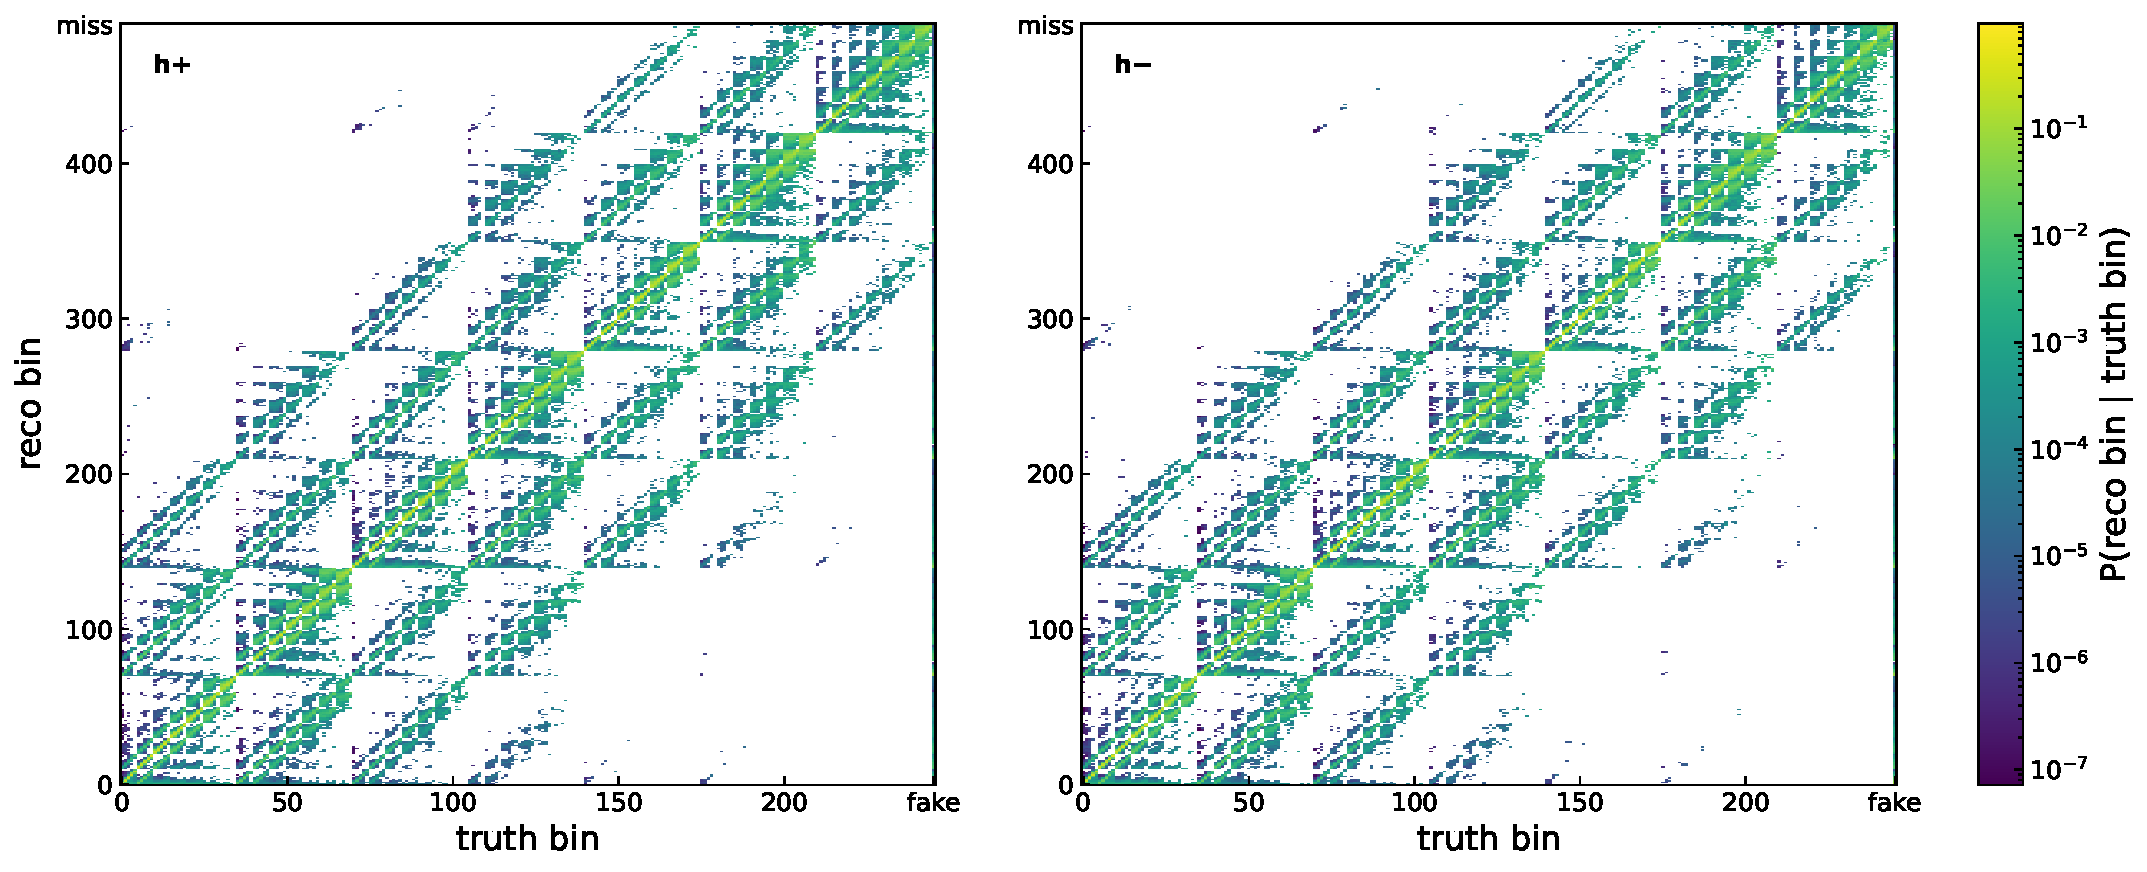
\includegraphics[width=0.92\textwidth]{figures/fig_alpha0p2_allfake_migration_matrix_z005_diagnostic_log_unstretched.pdf}
  \caption{Diagnostic/provisional all-fake migration matrix for the near-electron opening-angle veto study. The positive- and negative-charge response matrices each have shape $(491,246)$, with rows 0--489 corresponding to physical reconstructed bins, row 490 to misses, columns 0--244 to physical truth bins, and column 245 to fakes. The matrix is column-normalized as $P(\mathrm{reco\ bin}\mid\mathrm{truth\ bin})$ and displayed on a logarithmic colour scale without stretching the one-bin fake and miss extensions. Central response and release products are unchanged.}
  \label{fig:unfolding:alpha0p2-allfake-migration-matrix}
\end{figure}

\begin{figure}[t]
  \centering
  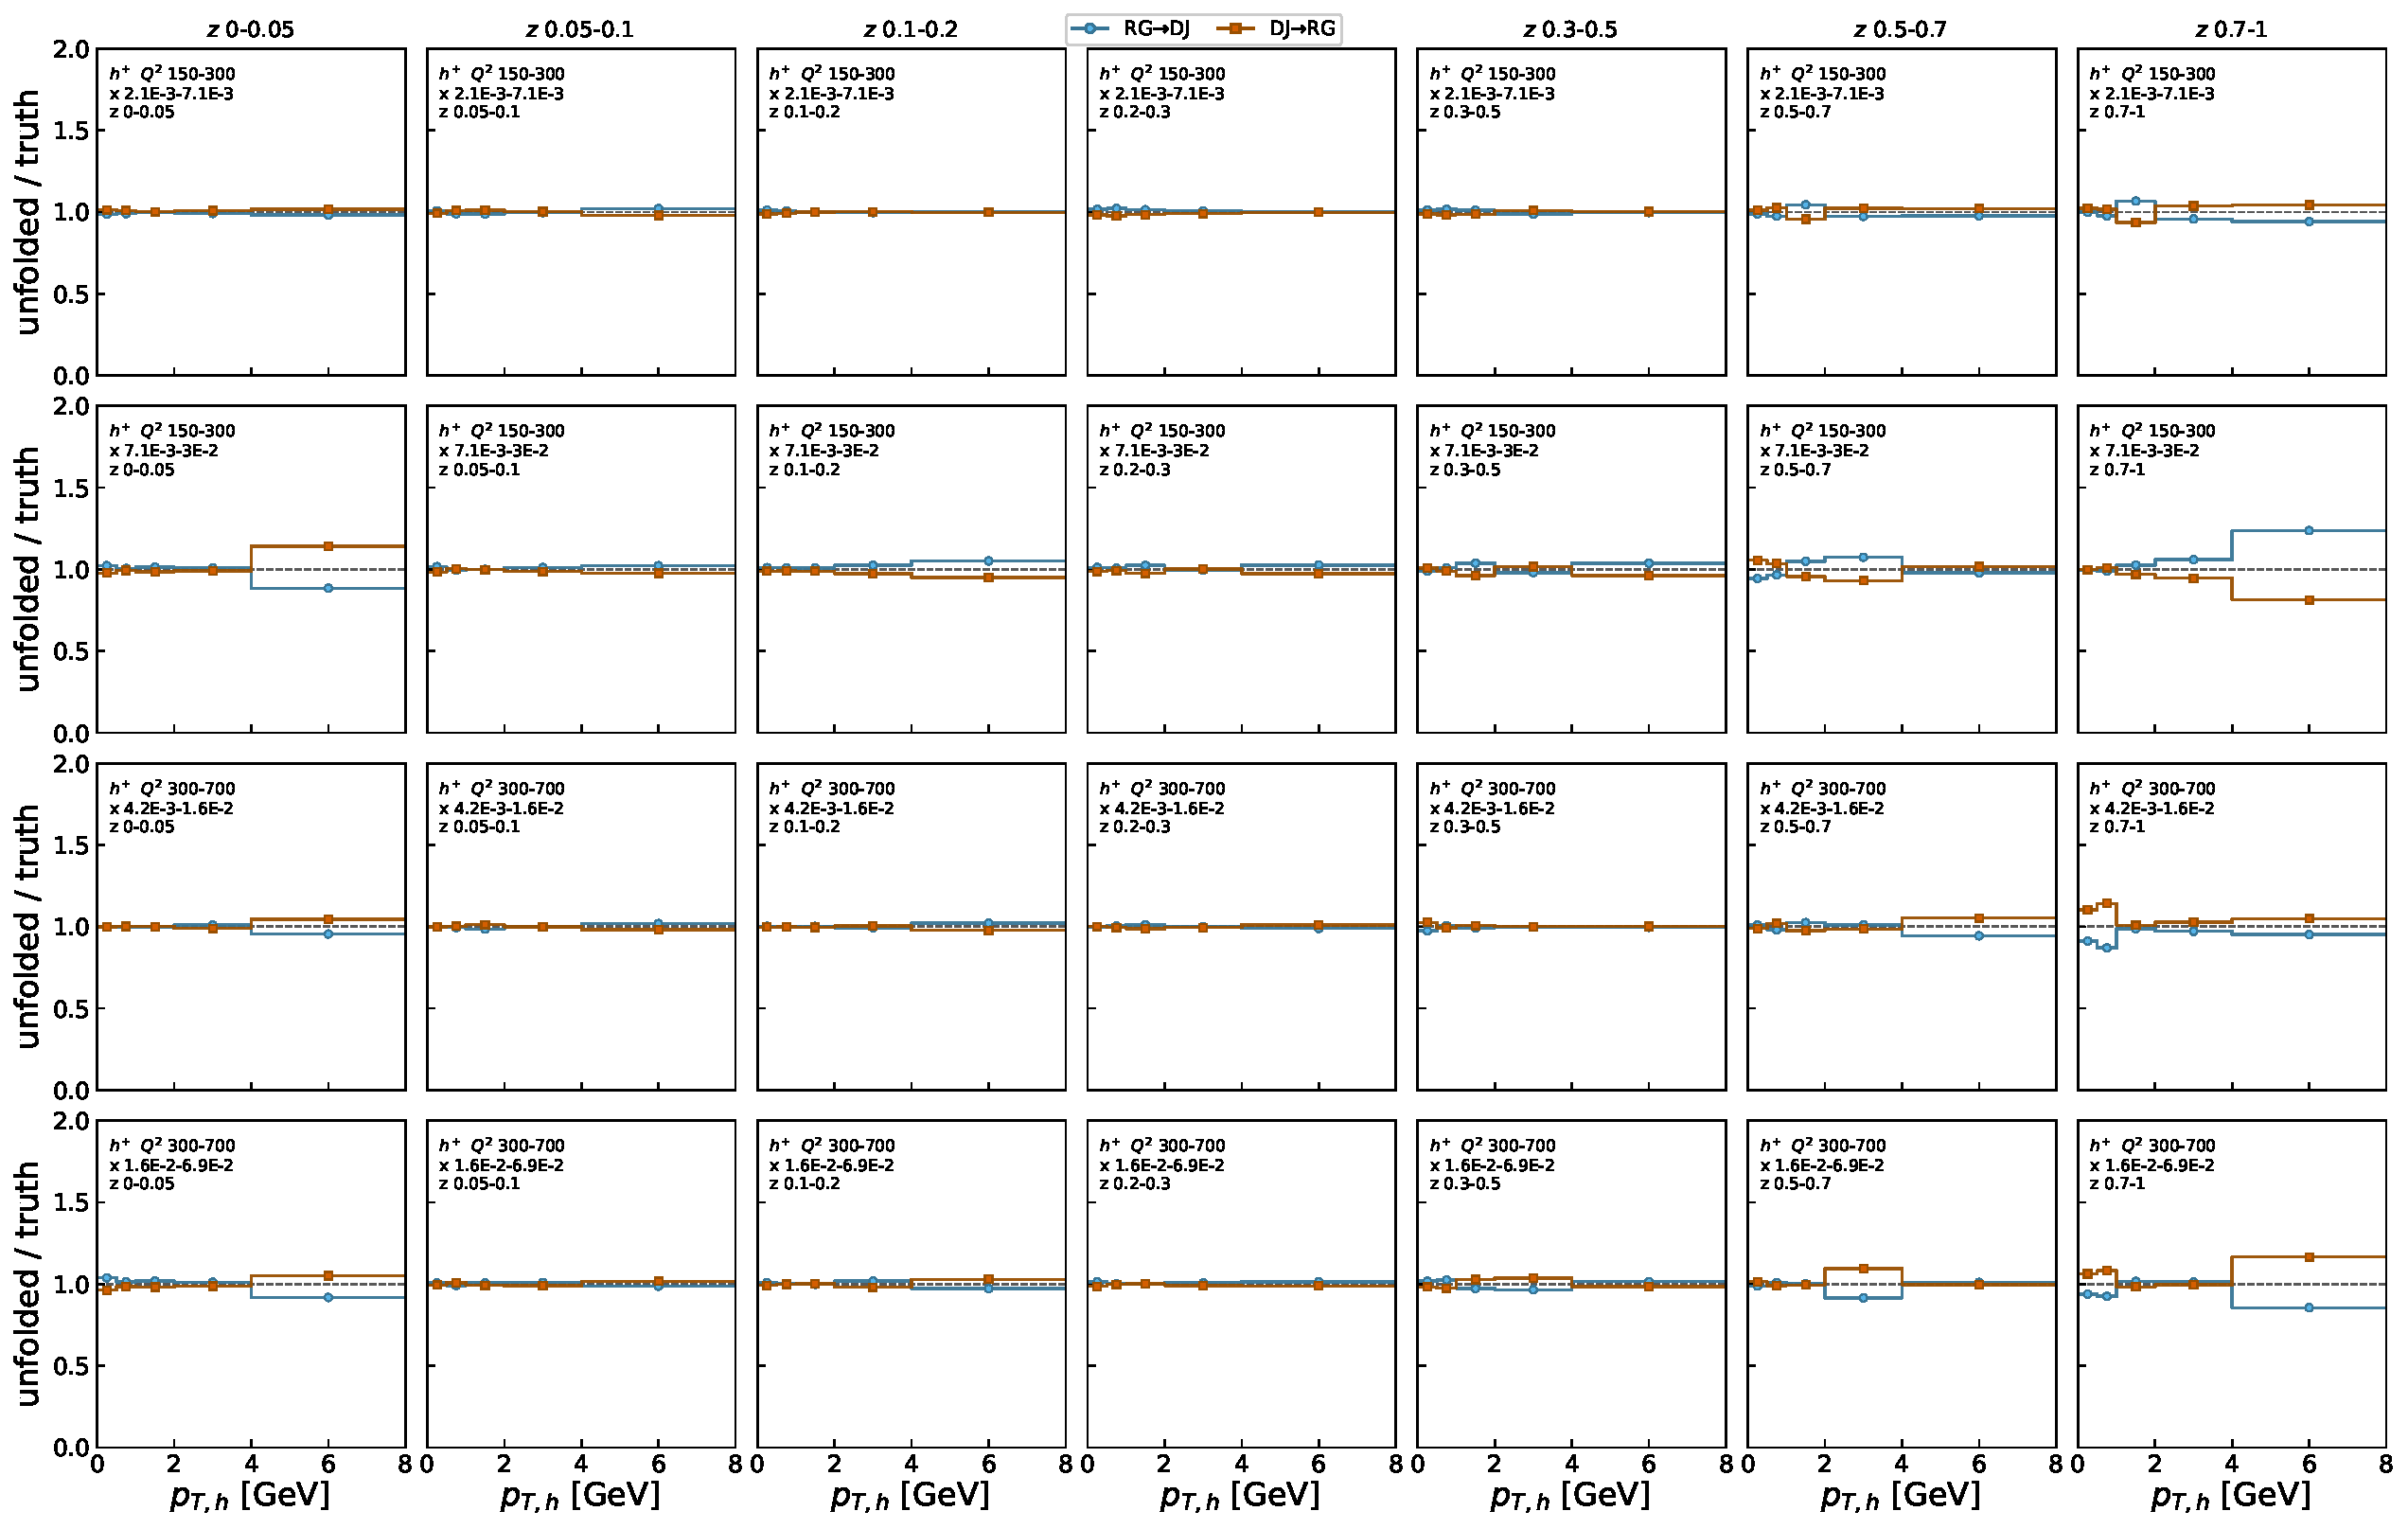
\includegraphics[width=0.92\textwidth]{figures/fig_ibu_crossclosure_7col_fullrange_z005.pdf}
  \caption{IBU cross-generator closure diagnostic in the canonical seven-column $\pTh$ layout, shown over the full ratio range 0--2. The plotted ratios are $\mathrm{DJ}\to\mathrm{RG}=N^{\mathrm{DJ\ reco,\ unfolded\ with\ RG\ response}}/N^{\mathrm{DJ\ truth}}$ and $\mathrm{RG}\to\mathrm{DJ}=N^{\mathrm{RG\ reco,\ unfolded\ with\ DJ\ response}}/N^{\mathrm{RG\ truth}}$. This is a cross-generator closure check only; no self-closure is included.}
  \label{fig:unfolding:ibu-crossclosure-fullrange}
\end{figure}

\begin{figure}[t]
  \centering
  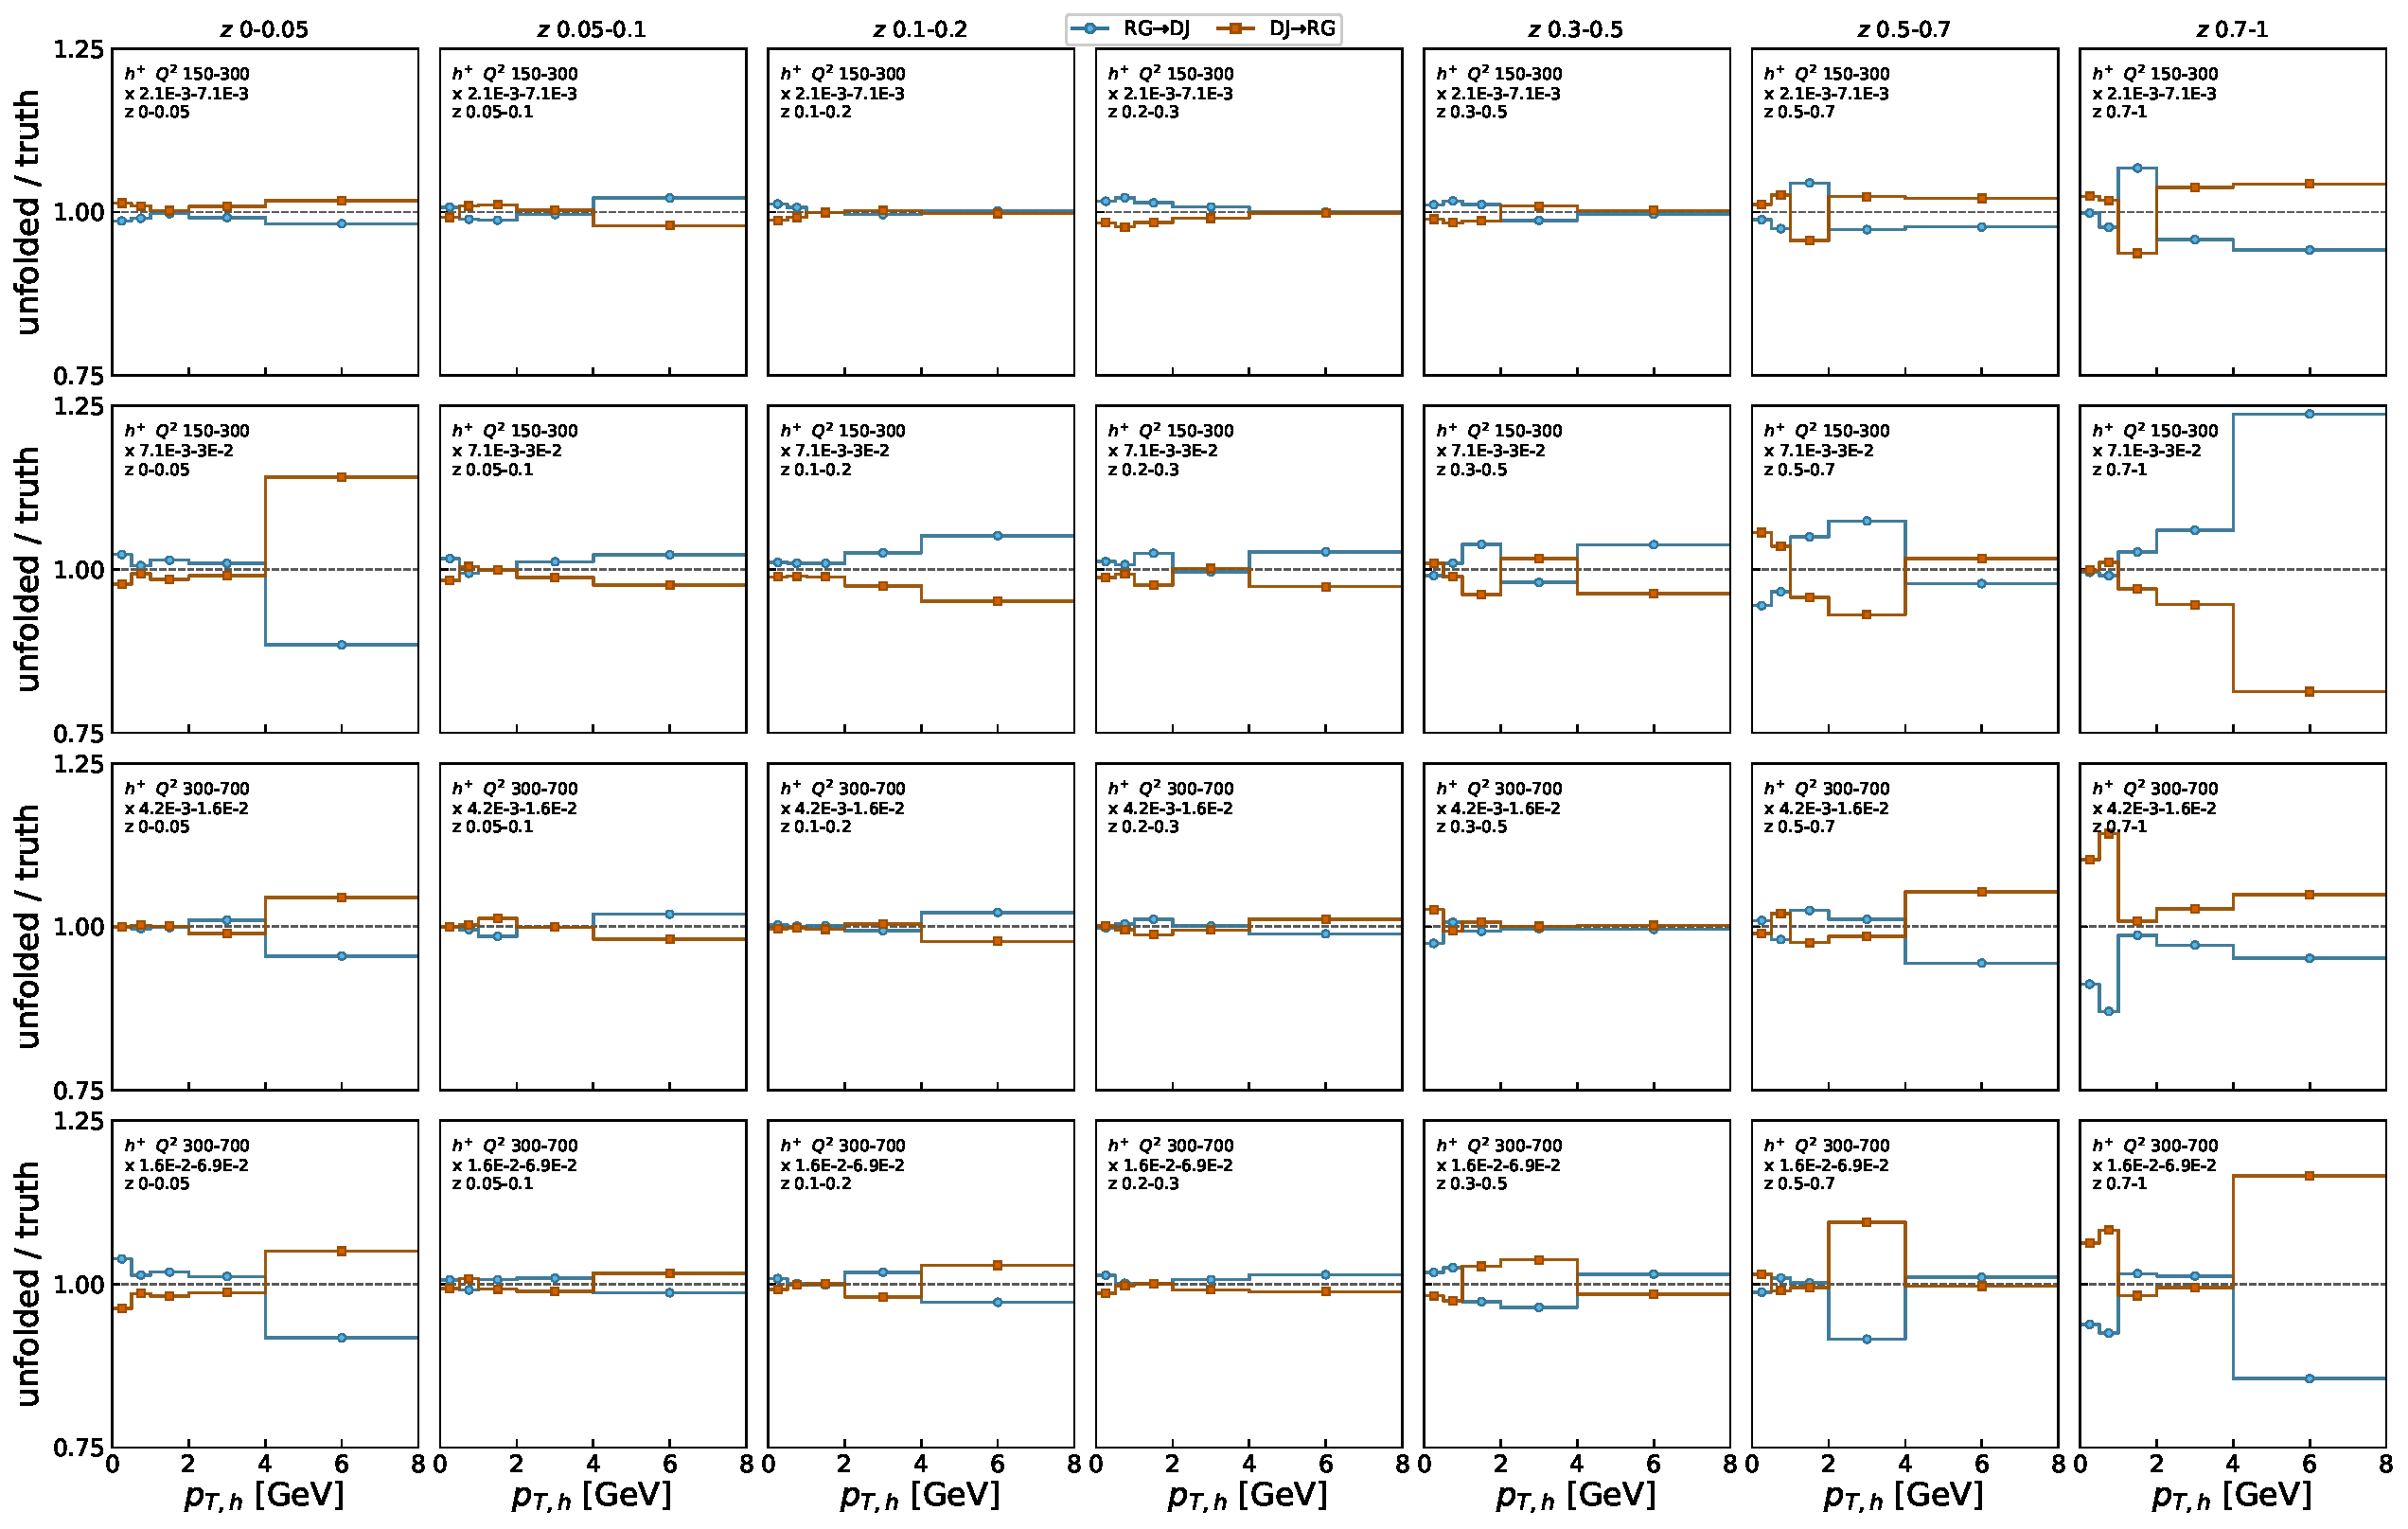
\includegraphics[width=0.92\textwidth]{figures/fig_ibu_crossclosure_7col_zoom_z005.pdf}
  \caption{Zoomed IBU cross-generator closure diagnostic in the canonical seven-column $\pTh$ layout, displaying the ratio range 0.75--1.25. Ratio definitions are the same as in Fig.~\ref{fig:unfolding:ibu-crossclosure-fullrange}; the diagnostic is cross-generator only and includes no self-closure component.}
  \label{fig:unfolding:ibu-crossclosure-zoom}
\end{figure}

\begin{figure}[t]
  \centering
  \begin{subfigure}[t]{0.95\textwidth}
    \centering
    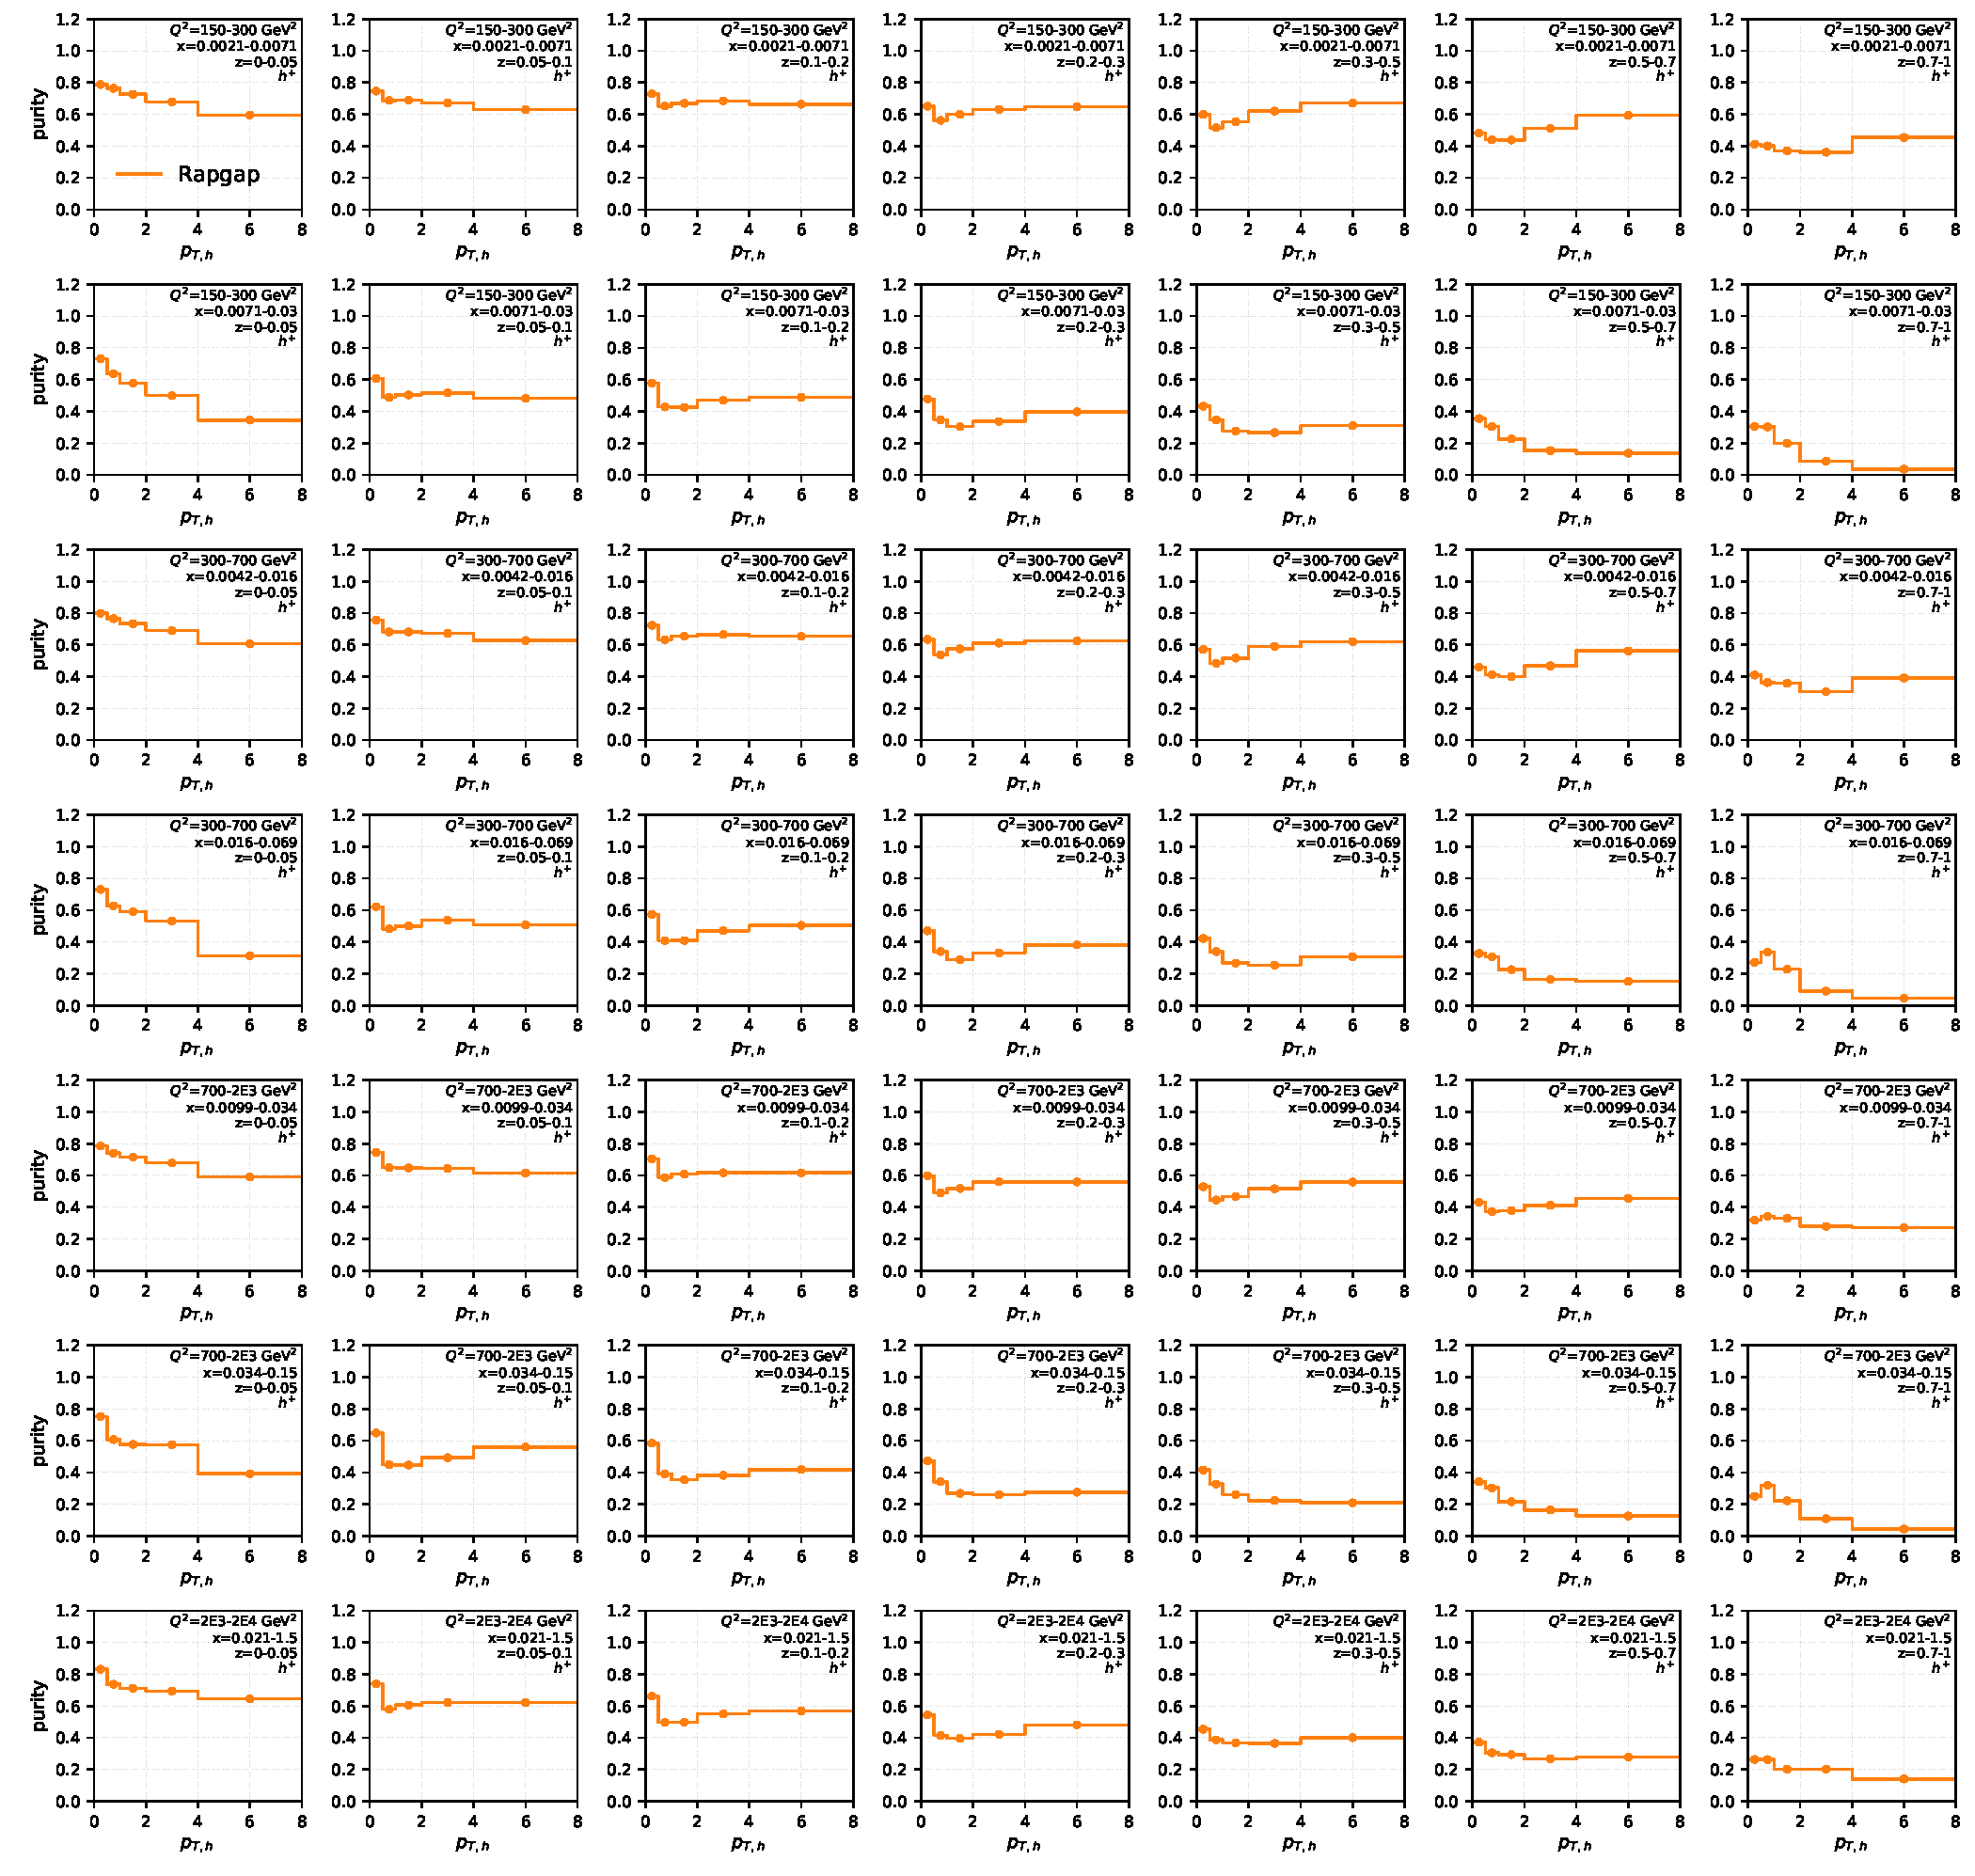
\includegraphics[width=\textwidth]{figures/fig_response_purity_hp_7col_20261007.pdf}
    \caption{Purity versus $\pTh$ for $\hplus$ in all bins, with the fake column included in $N_{\mathrm{rec}}$.}
  \end{subfigure}
  \hfill
  \begin{subfigure}[t]{0.95\textwidth}
    \centering
    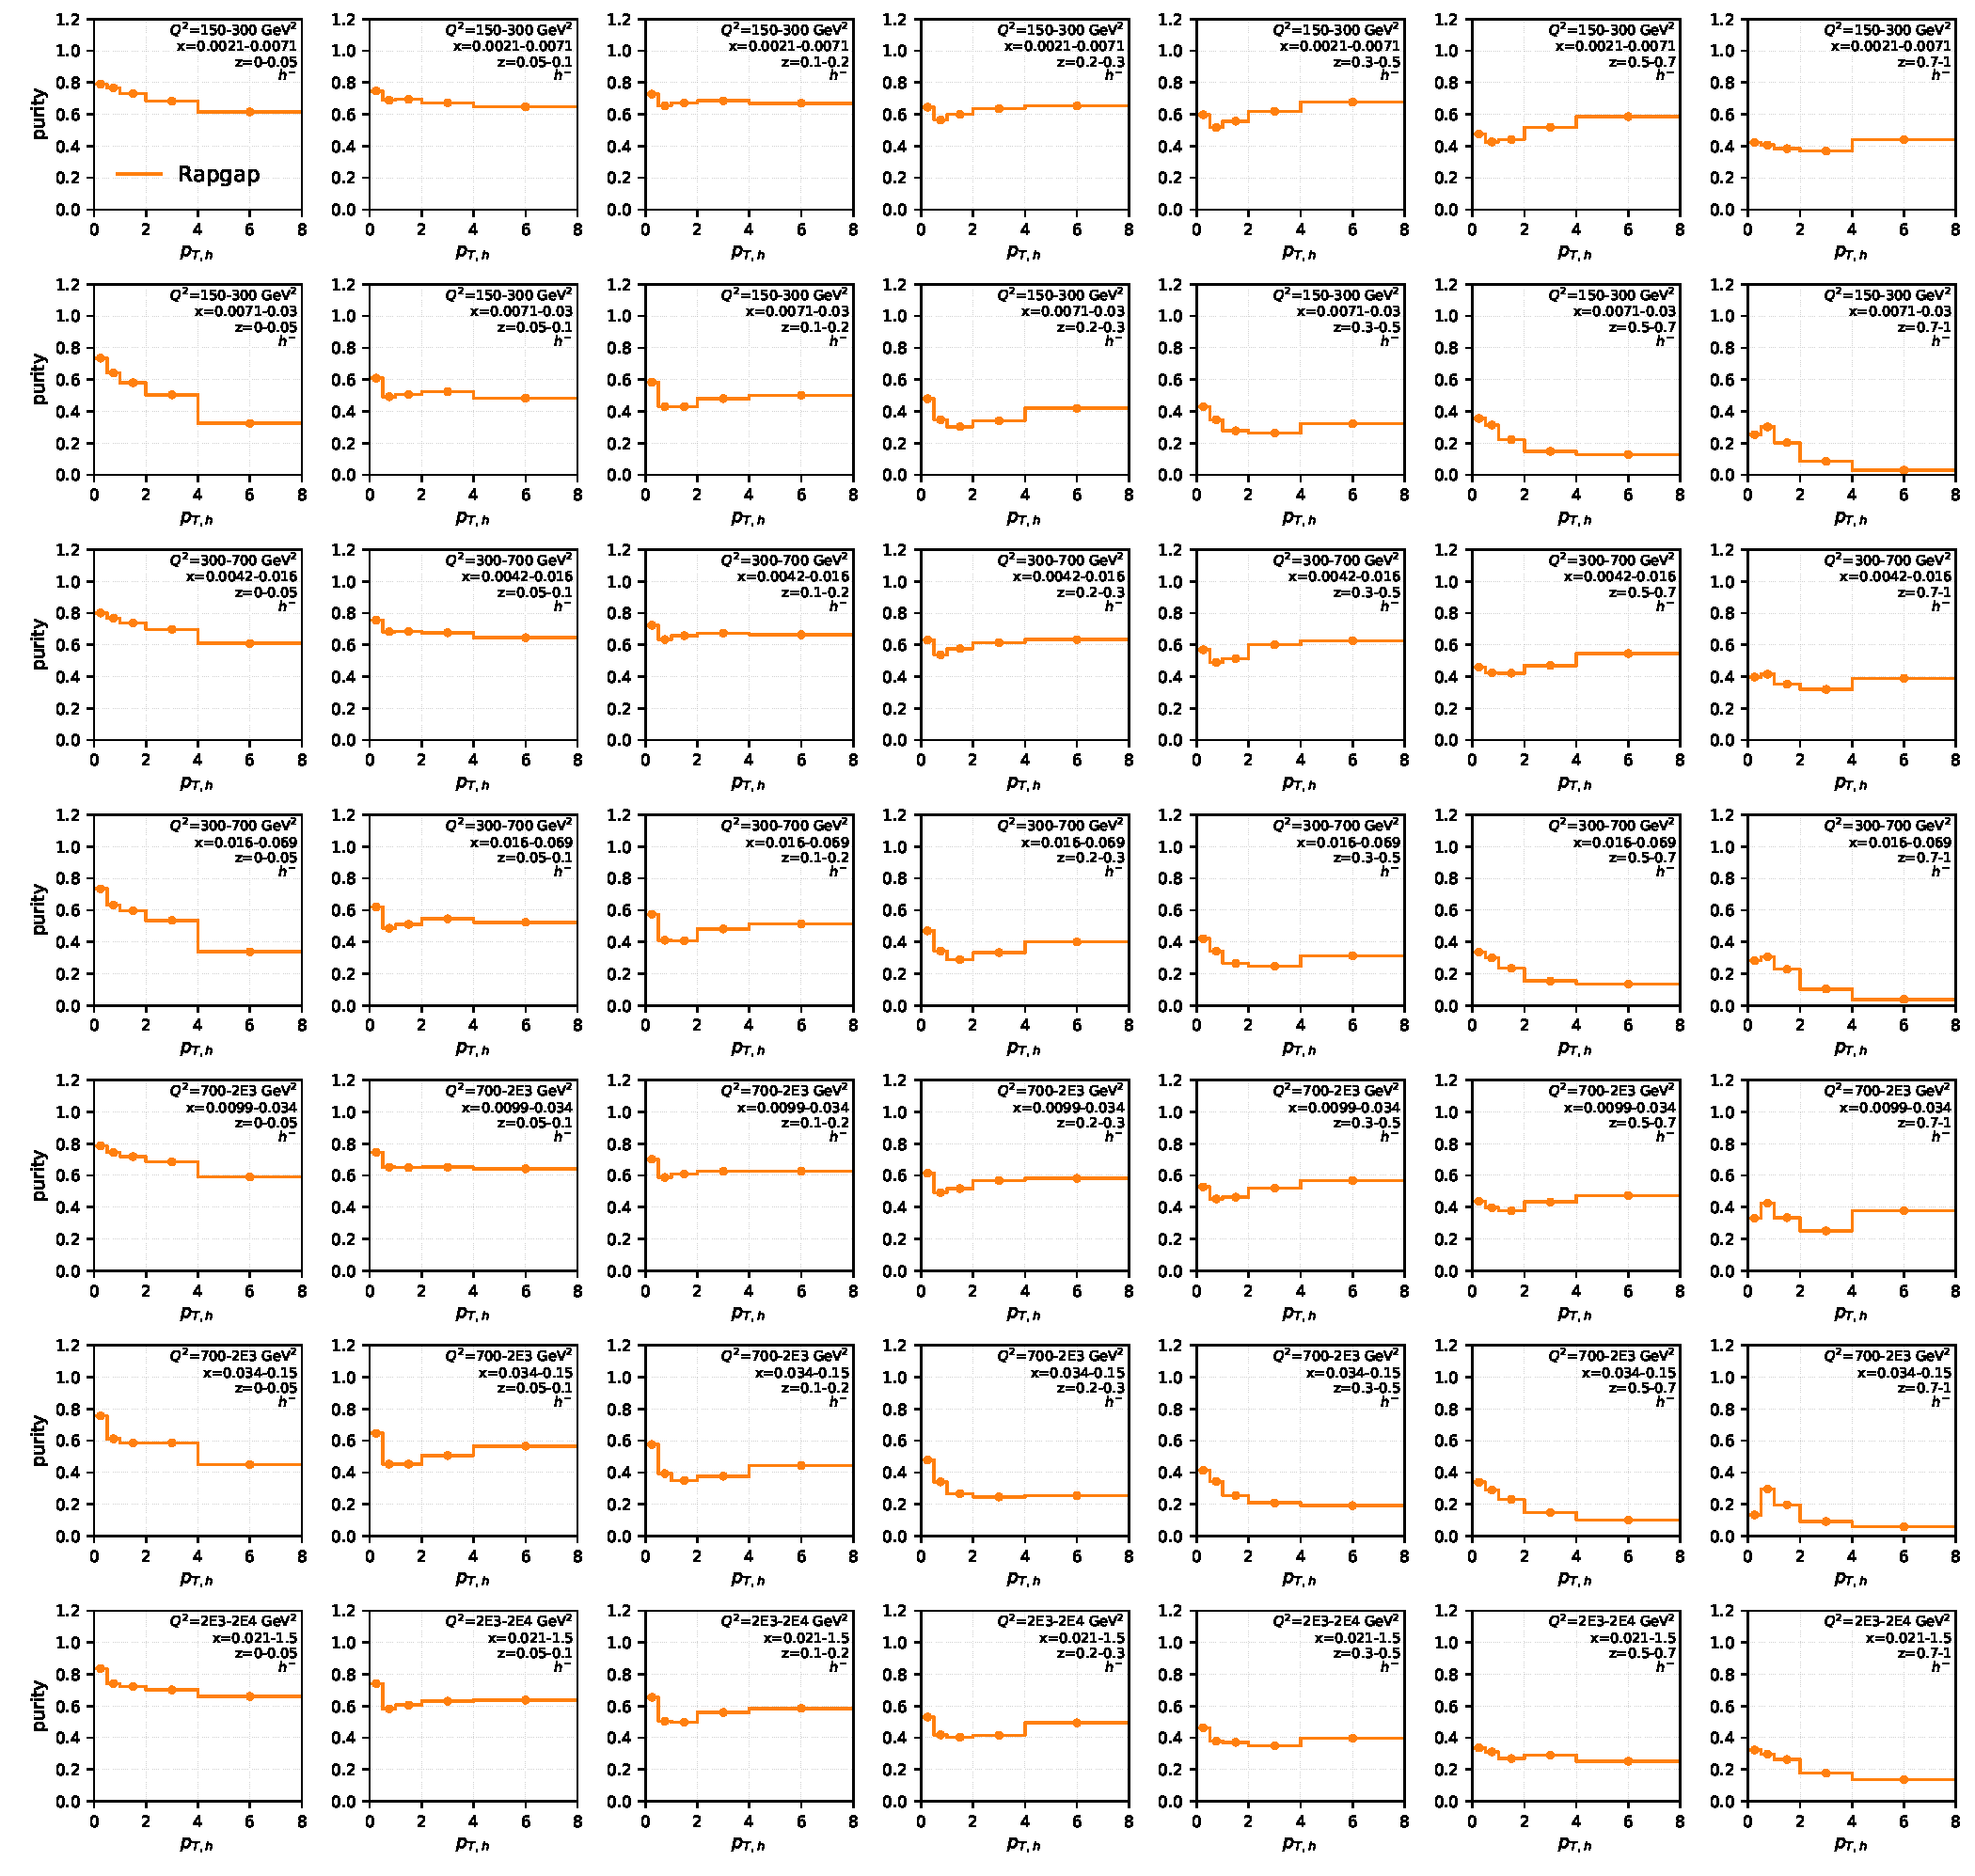
\includegraphics[width=\textwidth]{figures/fig_response_purity_hm_7col_20261007.pdf}
    \caption{$\hminus$, with the fake column included in $N_{\mathrm{rec}}$.}
    \label{fig:unfolding:alpha0p2-purity-hm}
  \end{subfigure}
  \caption{Purity versus $\pTh$ for $\hplus$ and $\hminus$ in all bins. The denominator $N_{\mathrm{rec}}$ includes the fake column.}
  \label{fig:unfolding:alpha0p2-purity}
\end{figure}

\begin{figure}[t]
  \centering
  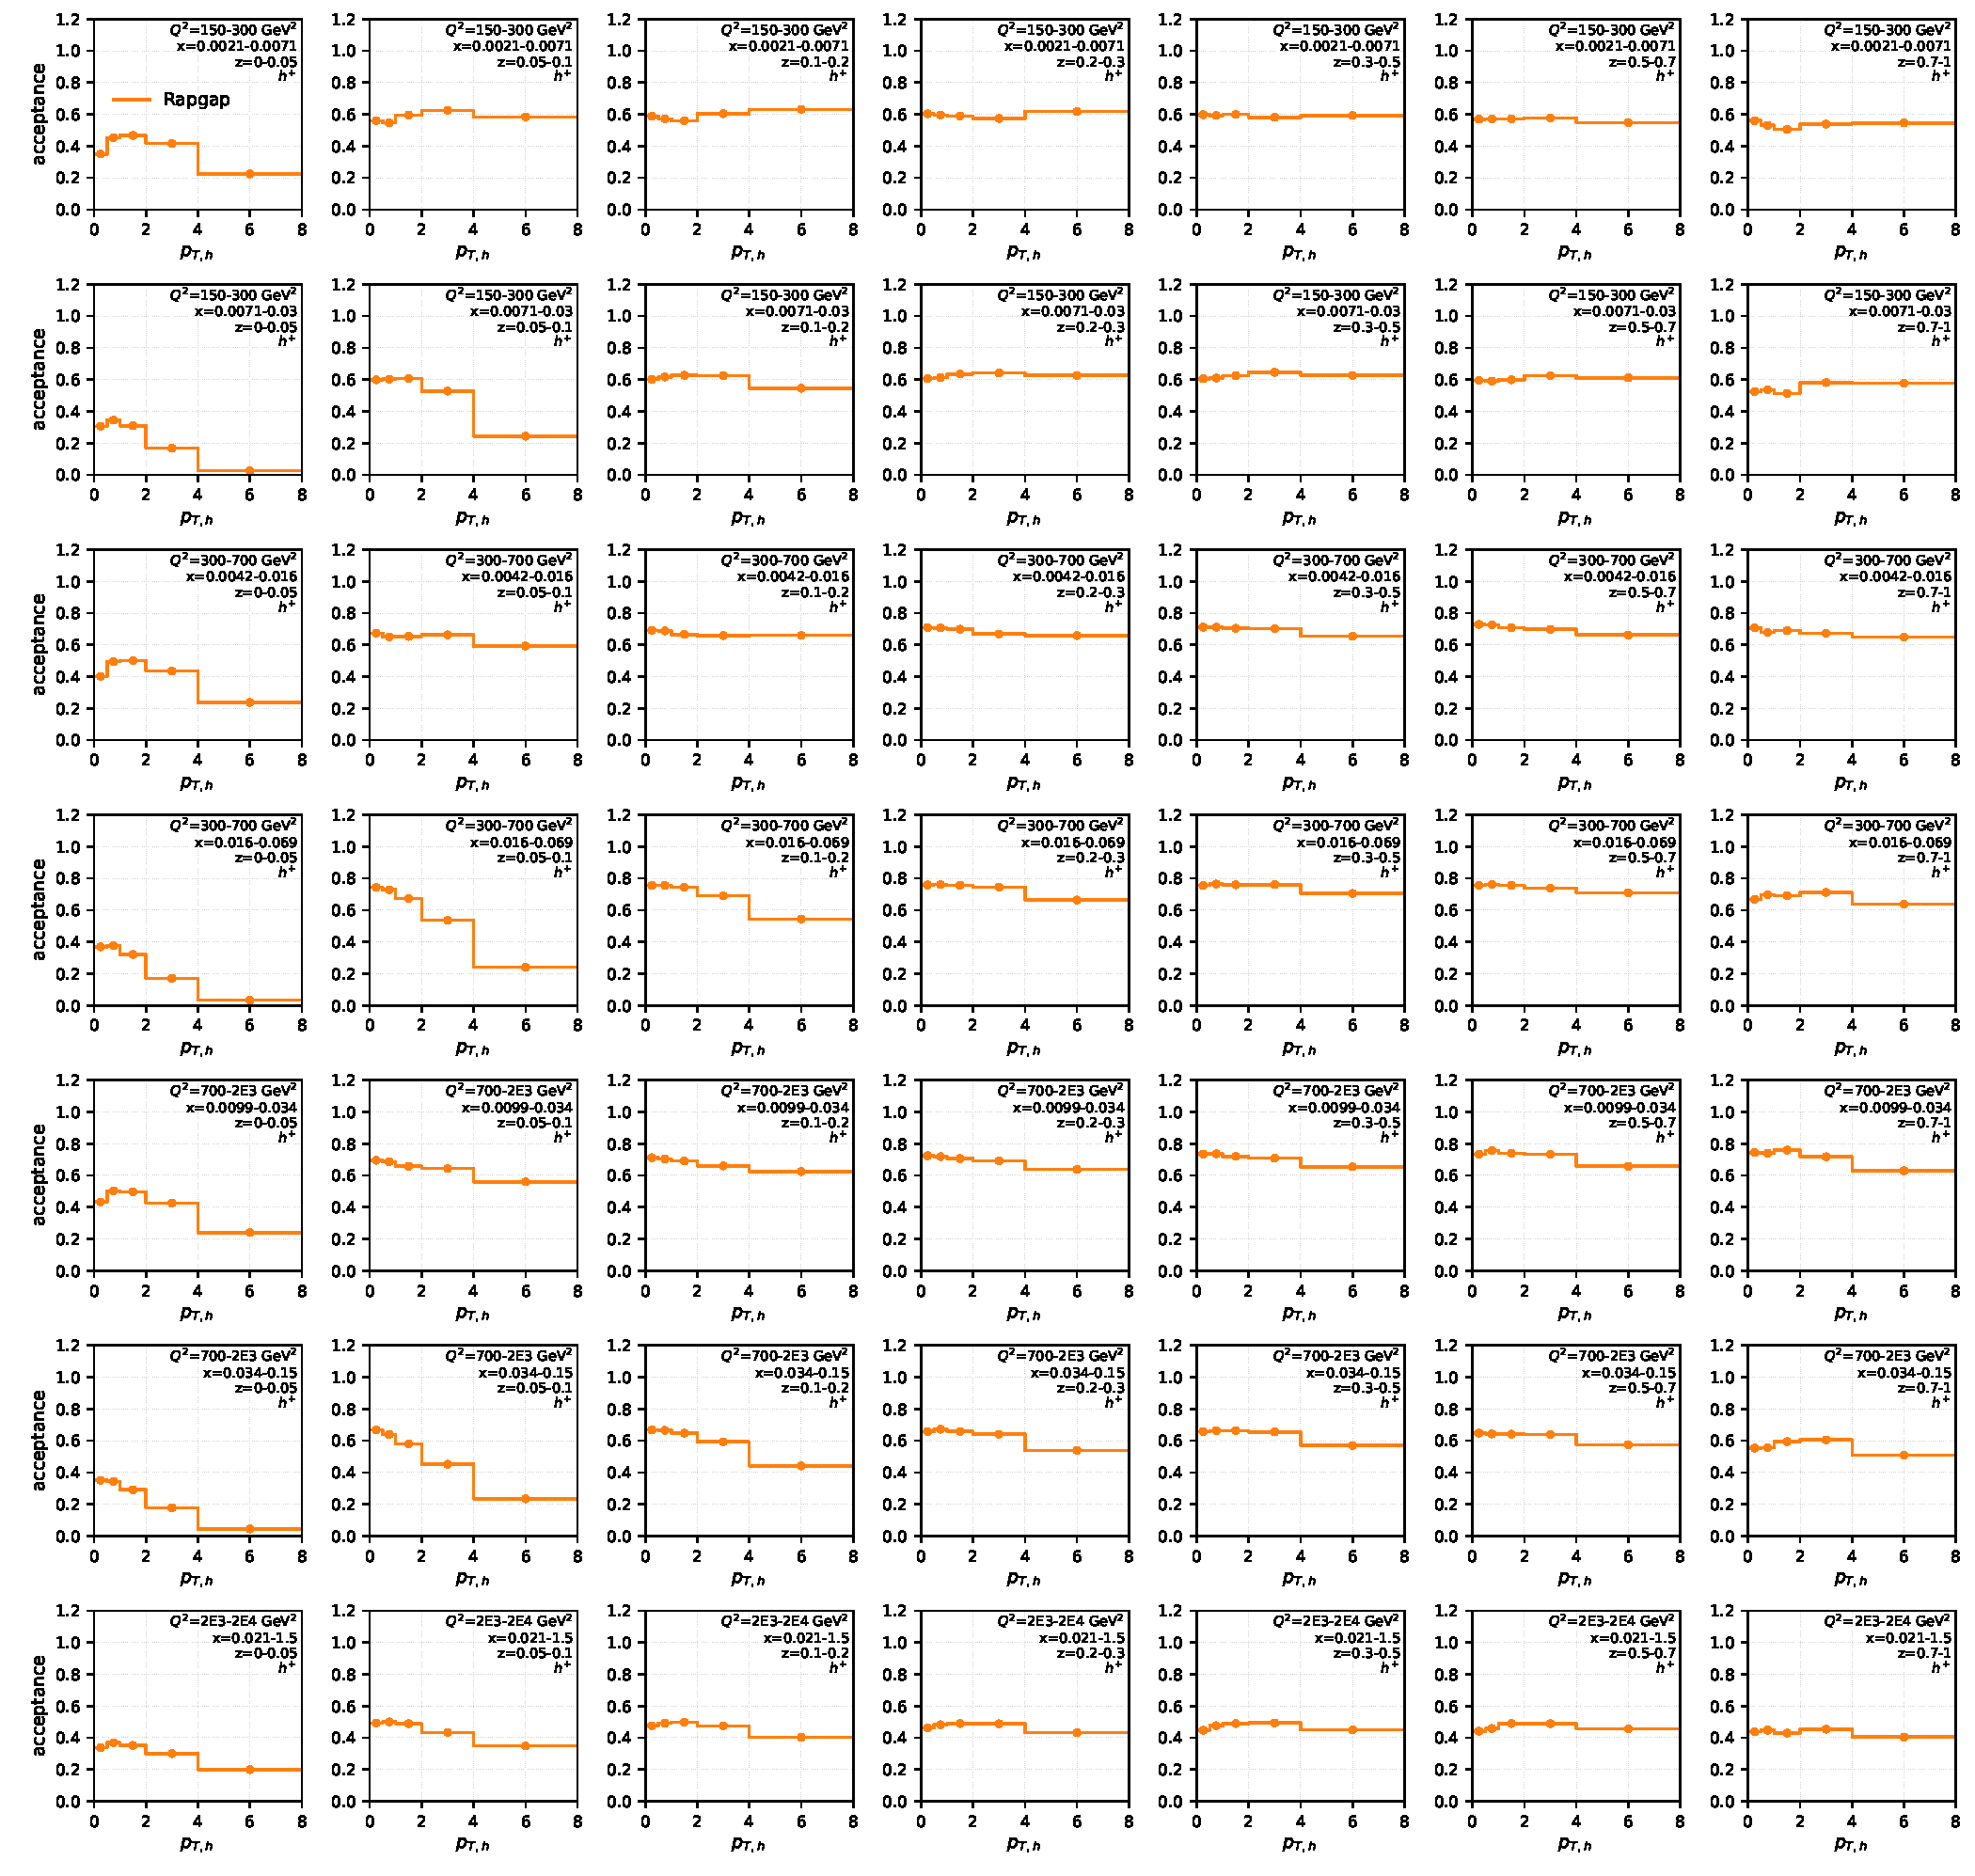
\includegraphics[width=0.92\textwidth]{figures/fig_response_acceptance_hp_7col_20261007.pdf}
  \caption{Acceptance versus $\pTh$ for $\hplus$ in all bins.}
  \label{fig:unfolding:alpha0p2-acceptance-hp}
\end{figure}

\begin{figure}[t]
  \centering
  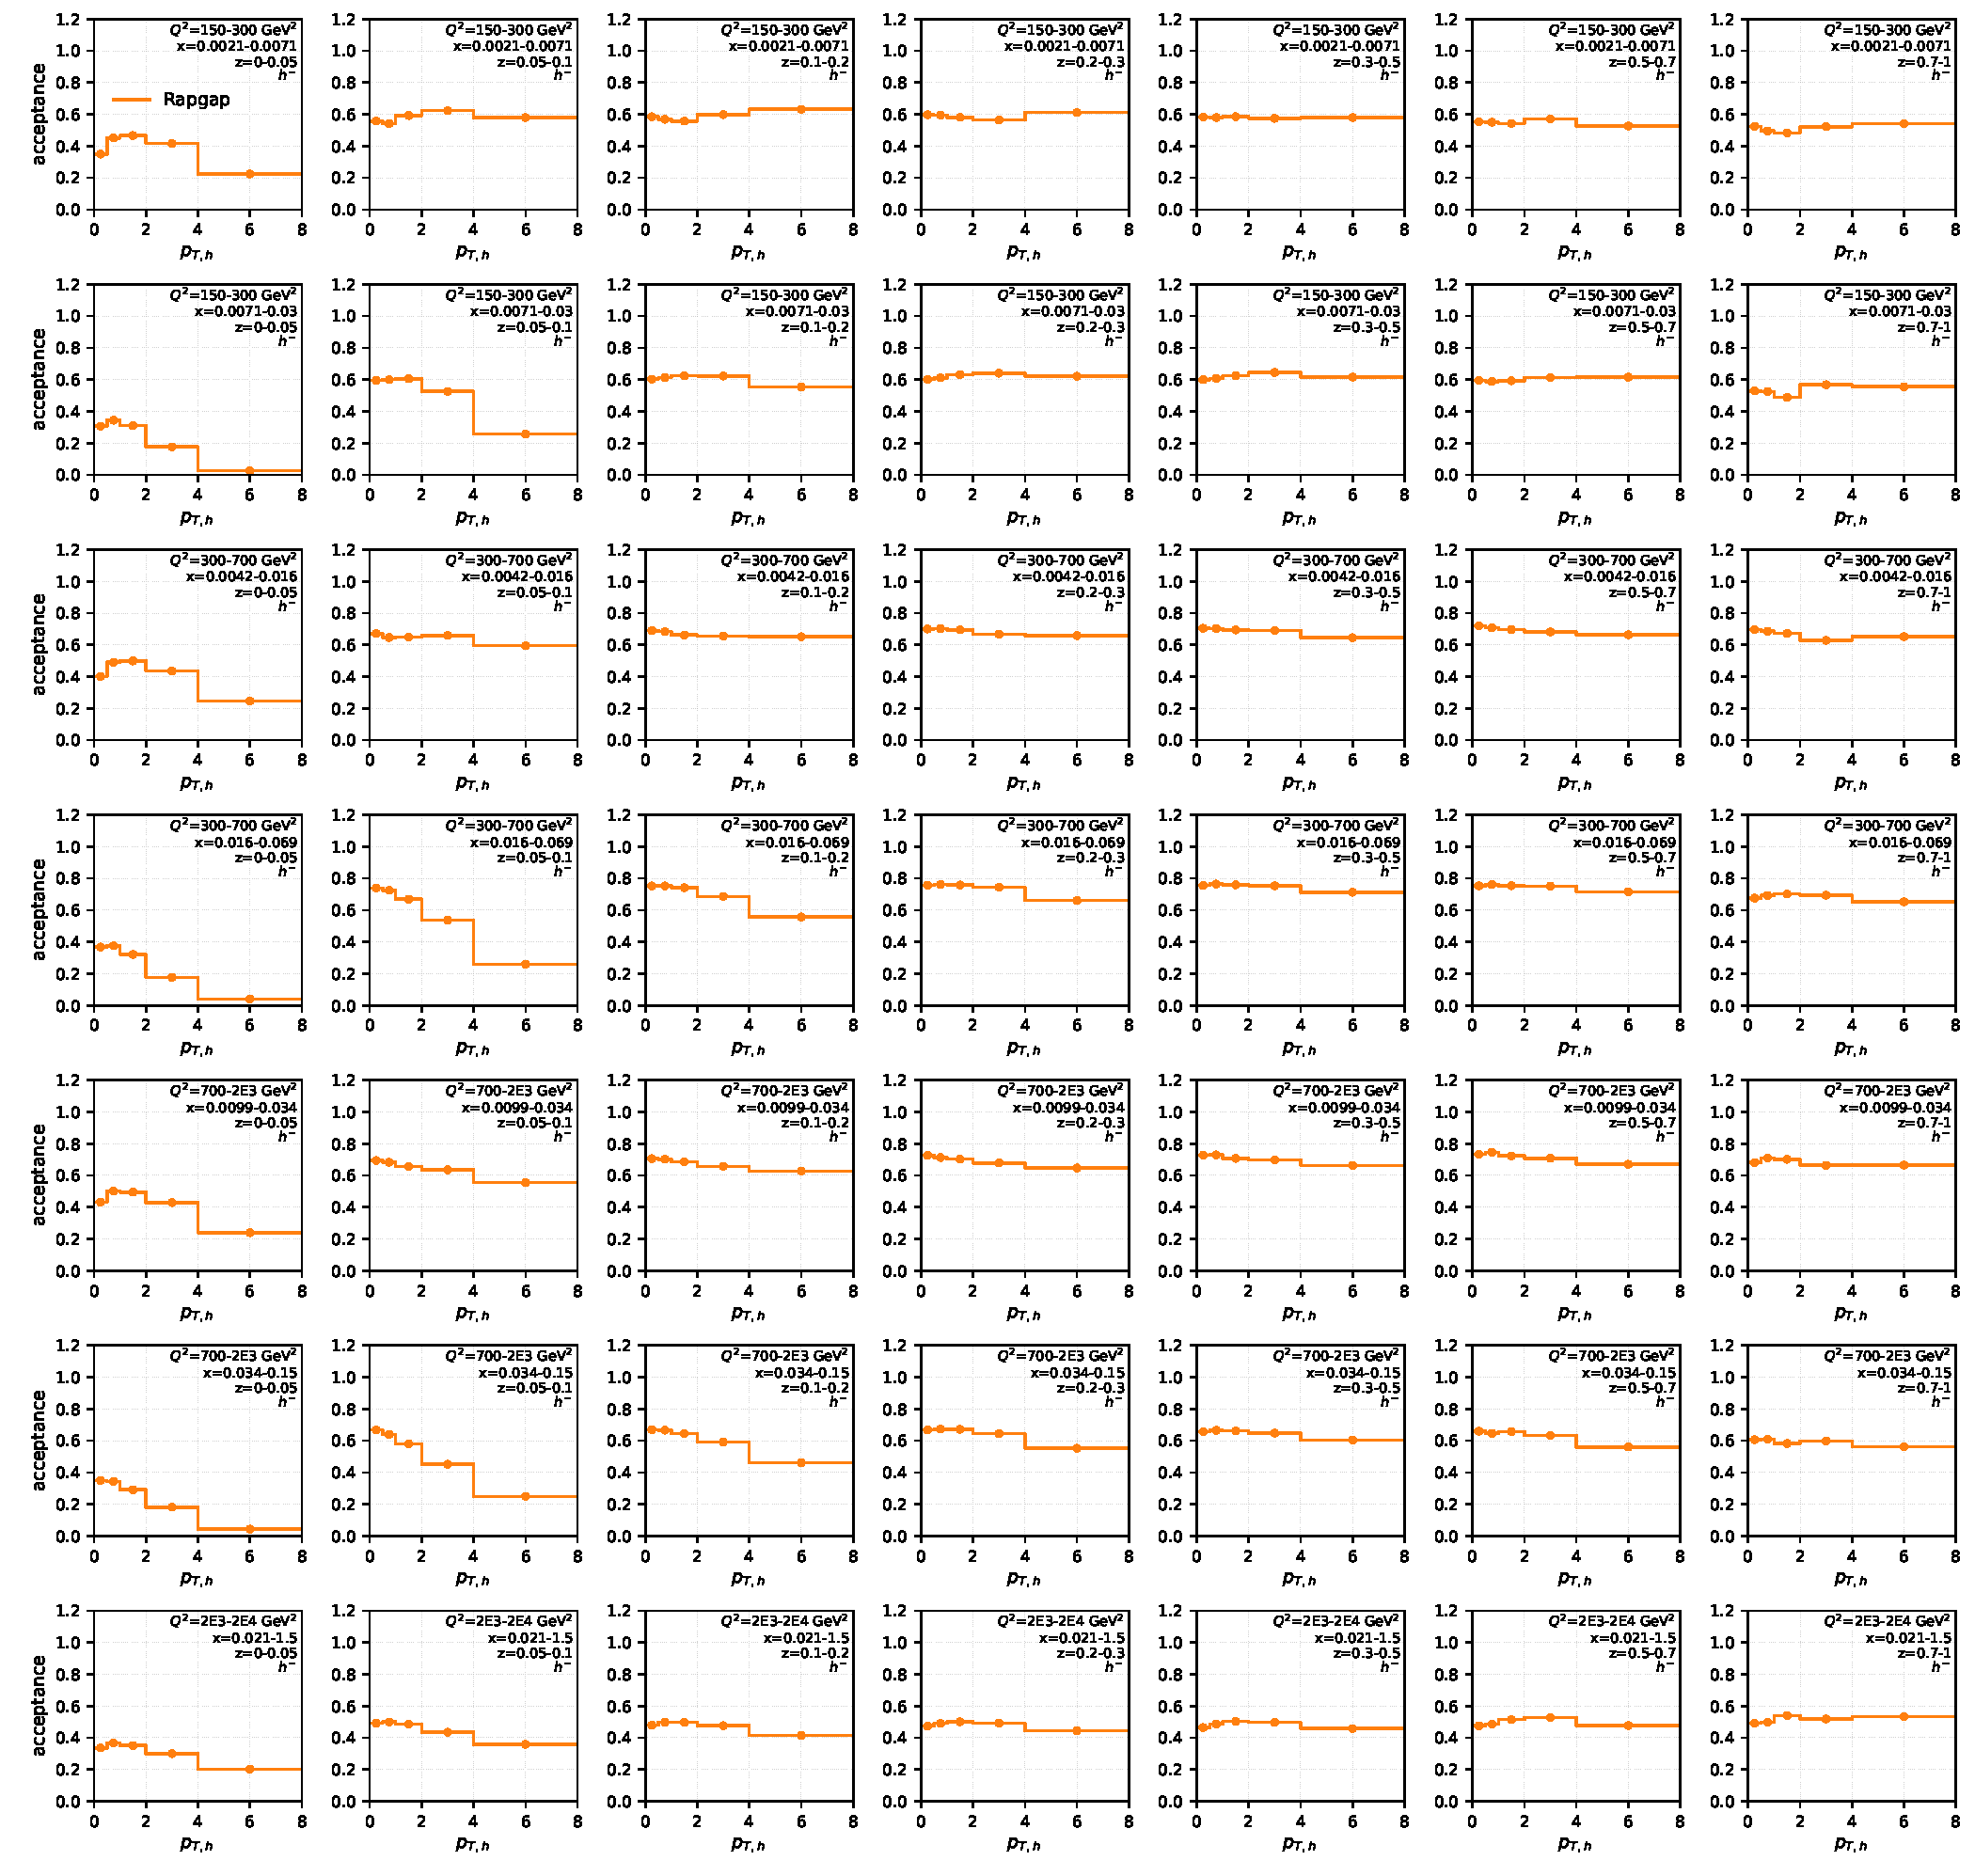
\includegraphics[width=0.92\textwidth]{figures/fig_response_acceptance_hm_7col_20261007.pdf}
  \caption{Acceptance versus $\pTh$ for $\hminus$ in all bins.}
  \label{fig:unfolding:alpha0p2-acceptance-hm}
\end{figure}

\subsection{Cross-check with TUnfold}
\label{sec:unfolding:tunfold-crosscheck}

Native ROOT/TUnfold v6 is retained as the validated second-method cross-check.  The iterative Bayesian unfolding, with the response's own generator-level prior and four iterations, is the final nominal method; the TUnfold result is diagnostic only.  The comparison uses the earlier detector-interaction-corrected basis without the electron cone, at raw level, which is also the basis of the existing figures in this section.  This superseded observable basis is retained for the diagnostic comparison; regeneration on the current basis is a separate pending item.

For TUnfold, $\tau=10^{-5}$ was selected with a 1\%-absolute-bias gate on both generator chains.  The delivered solution is $\max(x,0)$; its one-sided clipping bias, $+0.028\%$ for $h^+$ and $+0.0107\%$ for $h^-$, is accounted for separately.  In a 1000-toy validation on identical toys, both methods were unbiased and the TUnfold statistical uncertainty was toy-validated, with toy-to-reported ratios of 0.975 and 0.969 for $h^+$ and $h^-$, respectively.  TUnfoldSys covariance-in-solve propagation gave total-full median uncertainties of 9.16\% and 10.10\%, compared with 8.19\% and 8.41\% in the release budget, with the excess attributed in the validation record.  The method-choice record is documented in \texttt{docs/unfolding/pmethod\_decision\_dossier\_2026-10-14.md}.

\begin{figure}[t]
  \centering
  \begin{subfigure}[t]{0.49\textwidth}
    \centering
    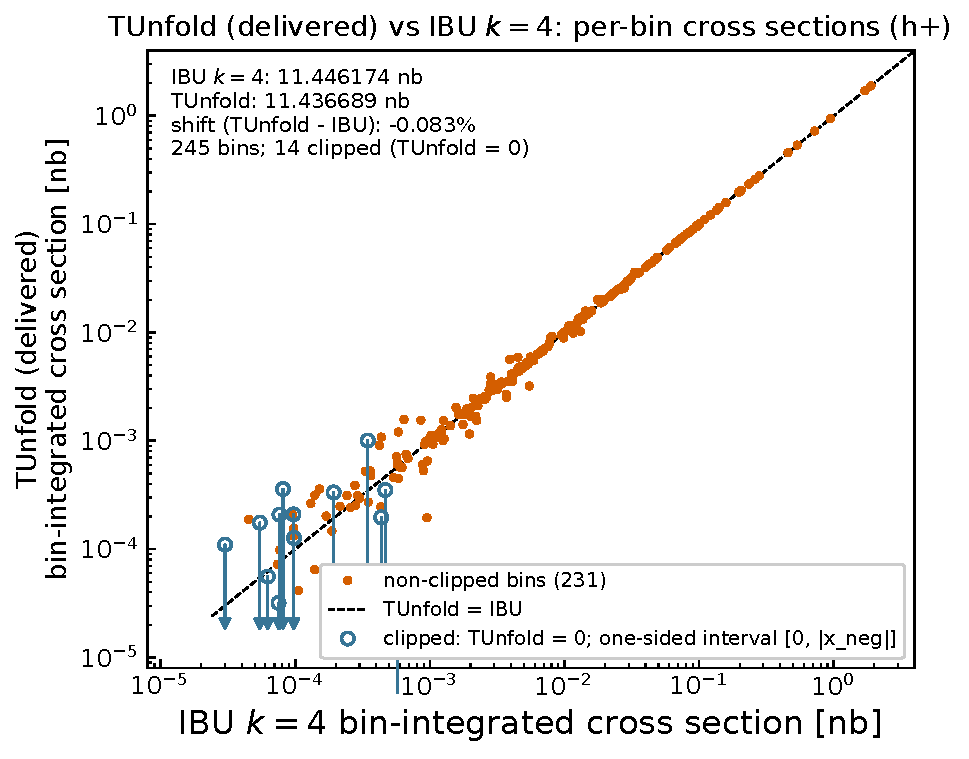
\includegraphics[width=\textwidth]{figures/fig_unfolding_tunfold_vs_ibu_scatter_z005_hplus.pdf}
    \caption{$\hplus$.}
  \end{subfigure}
  \hfill
  \begin{subfigure}[t]{0.49\textwidth}
    \centering
    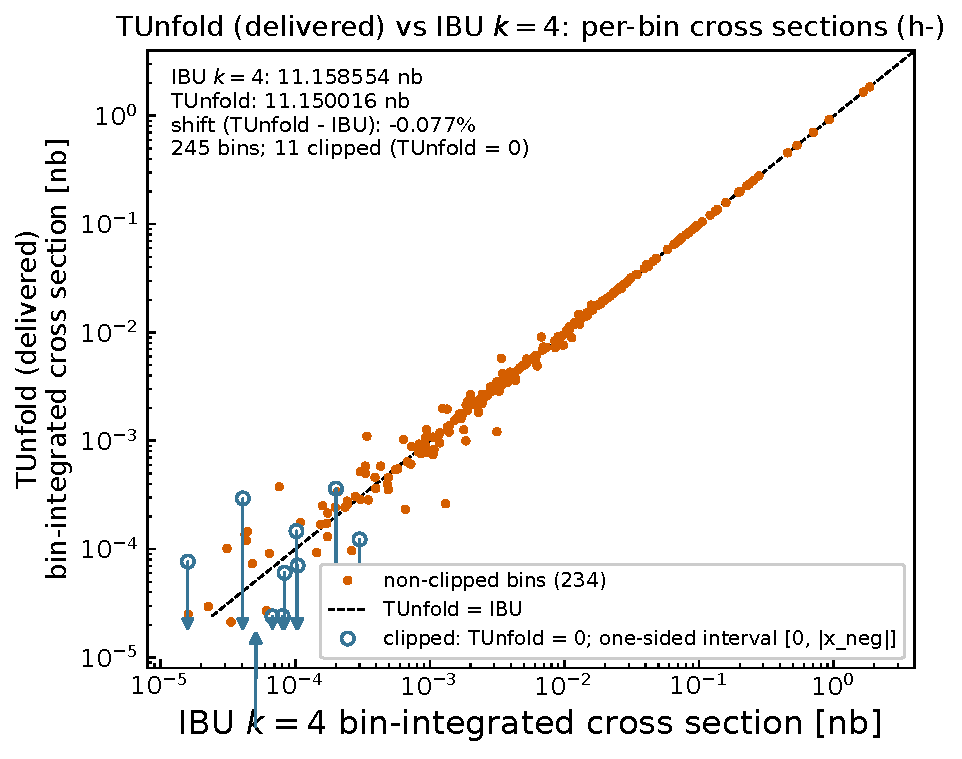
\includegraphics[width=\textwidth]{figures/fig_unfolding_tunfold_vs_ibu_scatter_z005_hminus.pdf}
    \caption{$\hminus$.}
  \end{subfigure}
  \caption{Per-bin logarithmic scatter comparison of the delivered TUnfold result with the nominal iterative Bayesian unfolding; the diagonal denotes equality.  These raw-level diagnostics use the superseded detector-interaction-corrected basis without the electron cone.  TUnfold uses $\tau=10^{-5}$ and delivers $\max(x,0)$: bins clipped from negative TUnfold values are shown as open markers at the one-sided upper value with limit-style arrows.  The comparison is retained as a diagnostic cross-check; the iterative Bayesian unfolding is nominal.}
  \label{fig:unfolding:tunfold-vs-ibu-scatter}
\end{figure}

\begin{figure}[t]
  \centering
  \begin{subfigure}[t]{0.49\textwidth}
    \centering
    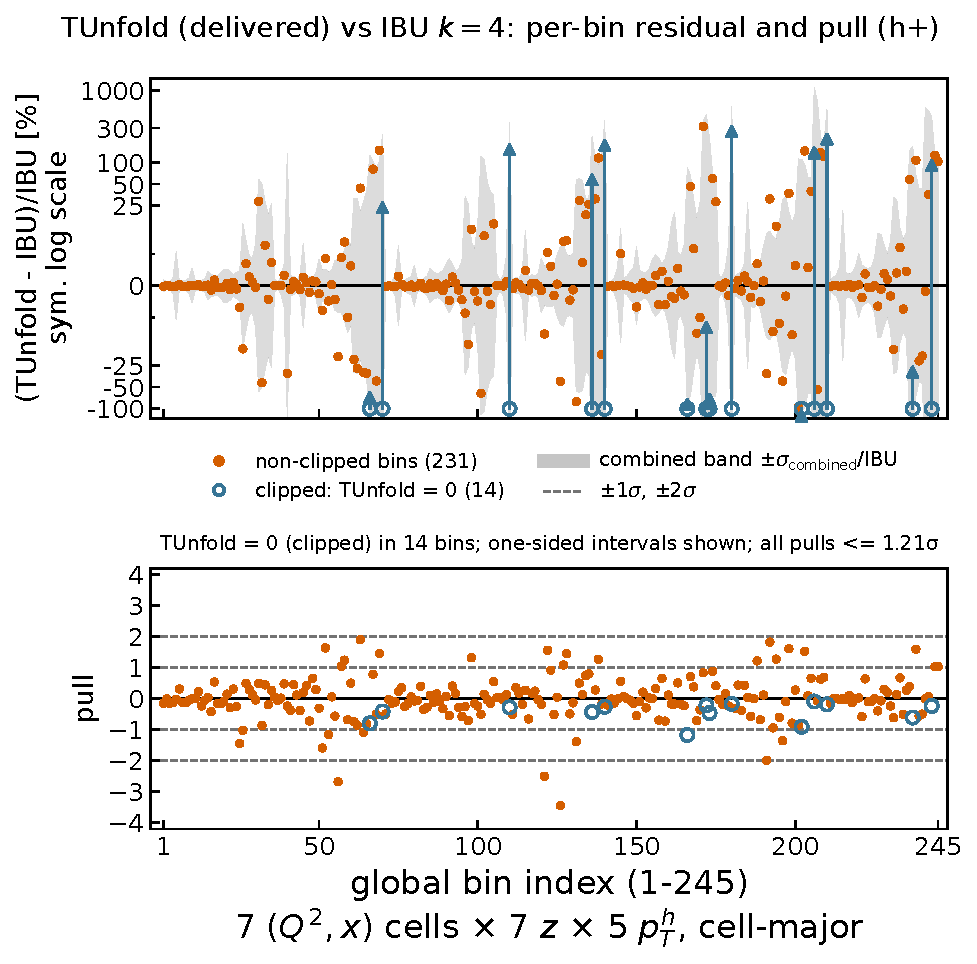
\includegraphics[width=\textwidth]{figures/fig_unfolding_tunfold_vs_ibu_residualpull_z005_hplus.pdf}
    \caption{$\hplus$.}
  \end{subfigure}
  \hfill
  \begin{subfigure}[t]{0.49\textwidth}
    \centering
    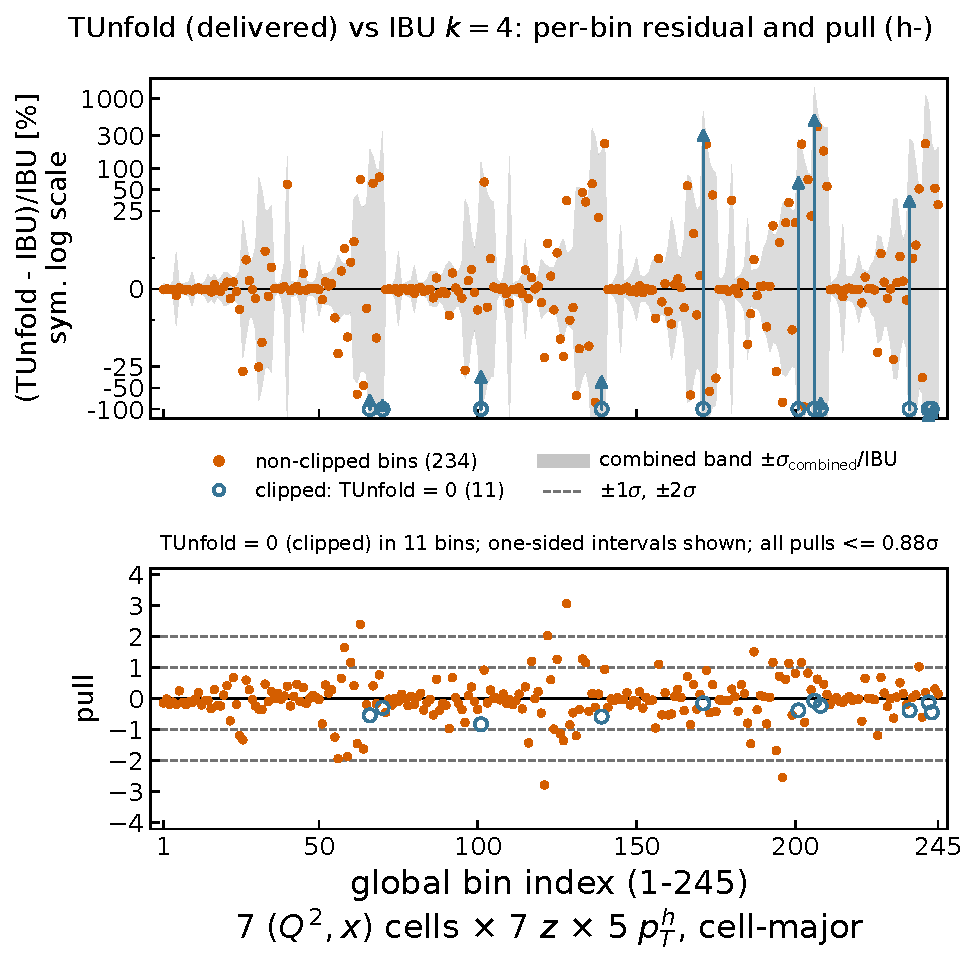
\includegraphics[width=\textwidth]{figures/fig_unfolding_tunfold_vs_ibu_residualpull_z005_hminus.pdf}
    \caption{$\hminus$.}
  \end{subfigure}
  \caption{Residuals and pulls by global bin index for the raw-level superseded-basis TUnfold diagnostic.  TUnfold uses $\tau=10^{-5}$ with delivered value $\max(x,0)$; clipped bins are open at $-100\%$ with one-sided interval bars.  Here $\mathrm{pull}=(x_{\mathrm{TU}}-x_{\mathrm{IBU}})/\sigma_{\mathrm{combined}}$.  The comparison is retained as a diagnostic cross-check with the iterative Bayesian unfolding as nominal; all 25 zero-delivered bins are statistically compatible with IBU, with maximum combined pulls of $1.21\sigma$ ($h^+$) and $0.88\sigma$ ($h^-$).}
  \label{fig:unfolding:tunfold-vs-ibu-residualpull}
\end{figure}

\begin{figure}[t]
  \centering
  \begin{subfigure}[t]{0.49\textwidth}
    \centering
    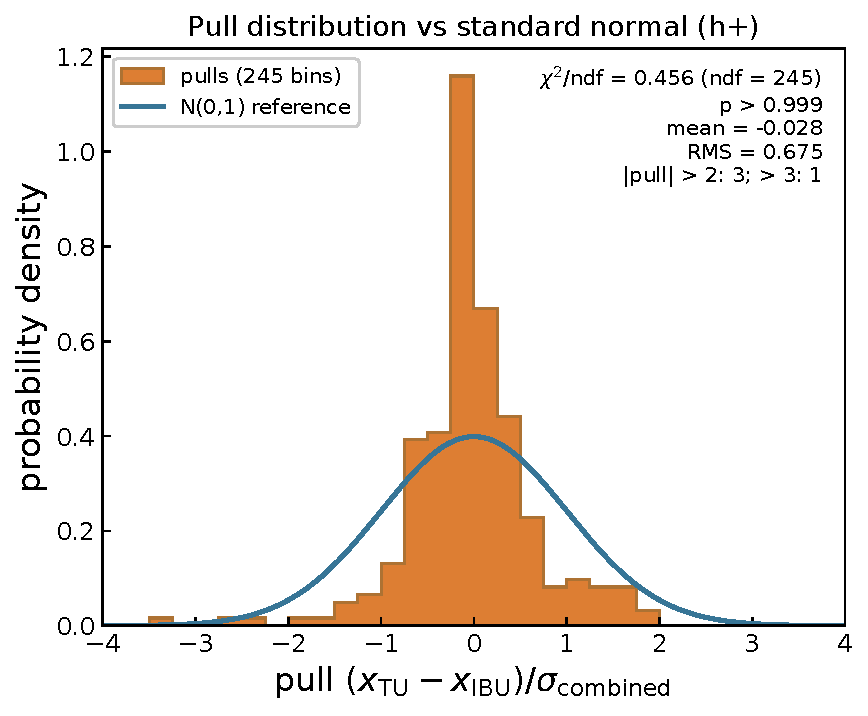
\includegraphics[width=\textwidth]{figures/fig_unfolding_tunfold_vs_ibu_pulls_z005_hplus.pdf}
    \caption{$\hplus$.}
  \end{subfigure}
  \hfill
  \begin{subfigure}[t]{0.49\textwidth}
    \centering
    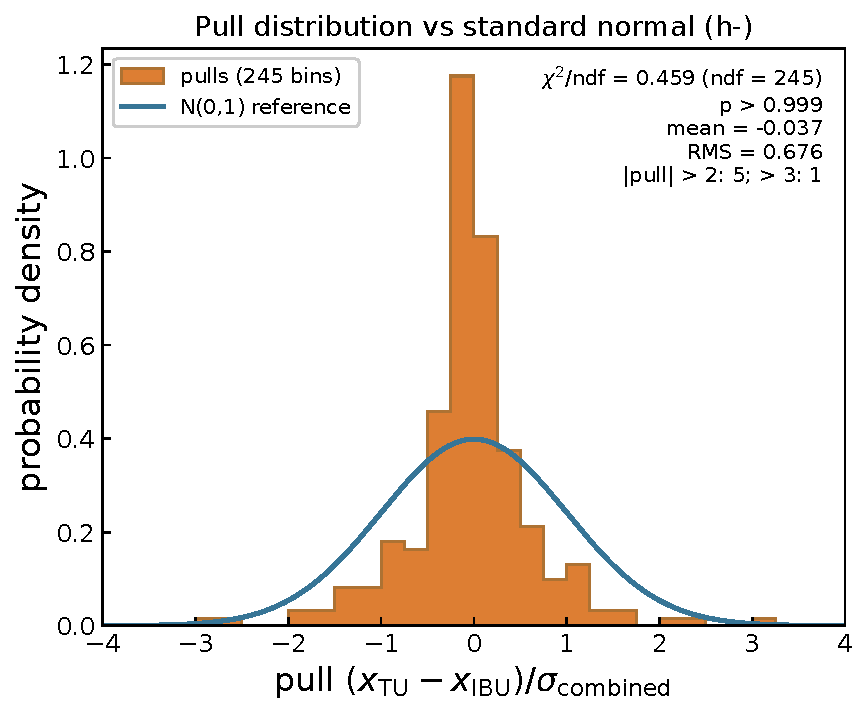
\includegraphics[width=\textwidth]{figures/fig_unfolding_tunfold_vs_ibu_pulls_z005_hminus.pdf}
    \caption{$\hminus$.}
  \end{subfigure}
  \caption{Distribution of $\mathrm{pull}=(x_{\mathrm{TU}}-x_{\mathrm{IBU}})/\sigma_{\mathrm{combined}}$ for the raw-level superseded-basis TUnfold diagnostic, compared with a standard-normal reference.  TUnfold uses $\tau=10^{-5}$ and the delivered prescription $\max(x,0)$; the comparison is retained as a diagnostic cross-check while the iterative Bayesian unfolding is nominal.  The diagonal-covariance consistency values are $\chi^2/\mathrm{ndf}=0.456$ and 0.459 for $h^+$ and $h^-$, with $p>0.999$.}
  \label{fig:unfolding:tunfold-vs-ibu-pulls}
\end{figure}



% =============================================================================
%  Section: Radiative Corrections
%  H1 Charged-Hadron SIDIS High-Q^2 Analysis Note
% =============================================================================
\section{Radiative Corrections}
\label{sec:radiative_corrections}

In addition to the hard scattering process itself, the incoming or the
outgoing lepton can emit real photons (QED radiation from the lepton
line).  Such photon emission changes the energy and the direction of the
scattered lepton and thereby shifts the event kinematics reconstructed
from it, so the measured cross section differs from the Born-level cross
section, i.e. the cross section of the hard scattering process with no
photon emitted from the lepton line.  A per-bin radiative correction
factor, $C_{\mathrm{rad}}$, converts the measured cross section to the
Born level.

\subsection{Definition and Derivation}
\label{sec:radiative_corrections:definition}

The correction is defined, separately in each published bin of the
analysis, as the ratio
\begin{equation}
  C_{\mathrm{rad}}(\mathrm{bin}) =
  \frac{\sigma_{\mathrm{nonrad}}(\mathrm{bin})}
       {\sigma_{\mathrm{rad}}(\mathrm{bin})},
\end{equation}
where $\sigma_{\mathrm{rad}}$ and $\sigma_{\mathrm{nonrad}}$ are the
generator-level cross sections that the same event generator predicts in
the same bin when photon emission from the lepton line is switched on and
off, respectively.  Each of the two cross sections is computed as the
weighted generator-level event yield in the bin, normalised by the
integrated luminosity of the corresponding simulated sample; only these
two simulated luminosities enter the ratio, and the data luminosity does
not enter at all.  The two samples are processed with an identical event
selection, identical binning, the same charged-hadron definition, and the
same event weighting, so that the ratio isolates the effect of the photon
radiation.  No detector simulation enters the derivation: the correction
is a purely generator-level quantity.

The correction is derived independently with two event generators, DJANGOH
\cite{Charchula:1994kf} and RAPGAP \cite{Jung:1993gf}, both of which are
interfaced to the same QED-radiation program, HERACLES
\cite{Kwiatkowski:1990es}, so that each generator can produce a matched
pair of samples with and without photon emission from the lepton line.
The DJANGOH correction is the one applied to the data.  The RAPGAP
correction is retained as an independent comparison and determines the
generator-related uncertainty of the correction
(Sec.~\ref{sec:radiative_corrections:uncertainties}).

Both samples of a pair are subject to the generator-level counterpart of
the analysis selection, so that the correction corresponds to the same
phase space and the same hadron population as the measurement.  The
selection comprises the DIS kinematic requirements of the measurement,
$150<\Qsq<20\,000~\GeVsq$ and $0.1<y<0.7$
(Sec.~\ref{sec:selection:final-events}); a minimum requirement on the
total hadronic final-state energy--momentum balance, $E-p_z>45~\GeV$; and
the current-hemisphere requirement that the hadron lie in the
current-fragmentation hemisphere of the $\gamma^{*}p$ center-of-mass
frame---the hemisphere into which the struck quark fragments, opposite
the proton-remnant direction---which corresponds to $x_F<0$ in the H1
sign convention used throughout this analysis
(Sec.~\ref{sec:selection:final-tracks}).  Every element of the selection,
in particular the current-hemisphere requirement, is imposed identically
on the radiative and the non-radiative sample.  The charged hadrons are
pions, kaons, and (anti)protons, the same truth-level hadron definition
as in the measurement (Sec.~\ref{sec:species_definition}), and the two
beam charges are combined in both samples, matching the combined
$e^{+}p$ and $e^{-}p$ data set of the measurement.

The current correction tables supersede all earlier versions.  They are the
releasebin tables, in which events are assigned to $(Q2esGen,x_{\mathrm{es,gen}})$
bins with the same definition of $x$ as the release binning.  The applied
DJANGOH14 table is
\path{/data/dust/group/h1/klesthen/BaryonAsym/sidis_highQ2/data/radiative/djangoh14_crad_releasebin_2026-10-09/crad_v3_xfgen_lt0_empz_gt45_nominal_490rows.csv};
the formal RAPGAP31 alternative is
\path{/data/dust/group/h1/klesthen/BaryonAsym/sidis_highQ2/data/radiative/rapgap_crad_releasebin_emfix_2026-10-09/crad_v3_xfgen_lt0_empz_gt45_nominal_490rows.csv}.
The current-hemisphere requirement and the EMPZ$>$45 convention are unchanged.

\subsection{Correction Factors}
\label{sec:radiative_corrections:values}

Integrated over all 490 published bins, the applied DJANGOH correction is
$1.142$ for $\hplus$ and $1.141$ for
$\hminus$.  The corresponding RAPGAP factors are $1.134$
for $\hplus$ and $1.134$ for $\hminus$.  For both
generators, every one of the 490 bins (245 per charge) has a finite
entry.  Integrated over all bins, the DJANGOH correction exceeds the
RAPGAP correction by $0.6419\%$ for $\hplus$ and $0.6499\%$ for
$\hminus$.

The precision of the correction itself is limited by the number of
simulated events.  The per-bin relative statistical uncertainty of the
applied correction has a median of $0.4272\%$ for $\hplus$ and
$0.4429\%$ for $\hminus$.

Table~\ref{tab:crad:integrated-variants} compares the integrated factors of
the applied mixed-beam correction with those of the two derived Born-target
variants, together with their integrated statistical uncertainties and,
where a RAPGAP31 counterpart exists, the integrated generator difference.
The two target variants are provisional diagnostics and are not applied to
any result in this note.

\begin{table}[h]
\centering
\small
\begin{tabular}{p{4.6cm}p{5.2cm}p{5.2cm}}
\toprule
Variant & $\hplus$ & $\hminus$ \\
\midrule
Mixed-beam (applied primary, DJANGOH14 releasebin)$^{a}$ &
  $1.142 \pm 0.000123$ (stat) $\pm 0.00728$ (gen) &
  $1.141 \pm 0.000124$ (stat) $\pm 0.00736$ (gen) \\
$e^{-}p$ WithZ (per-beam target, DJANGOH14)$^{b}$ &
  $1.148 \pm 0.000151$ (stat) $\pm 0.0106$ (gen) &
  $1.147 \pm 0.000151$ (stat) $\pm 0.0101$ (gen) \\
NoZ photon-Born $C_{\gamma\mathrm{Born}}$ (DJANGOH14)$^{c}$ &
  $1.041 \pm 0.000143$ (stat) &
  $1.040 \pm 0.000144$ (stat) \\
\bottomrule
\end{tabular}

{\footnotesize
$^{a}$The applied primary: the per-bin DJANGOH14 releasebin tables applied
to the Born release (Sec.~\ref{sec:radiative_corrections:application}); the
Born level is the luminosity-weighted mixture of the $e^{+}p$ and $e^{-}p$
Born cross sections.

\smallskip
$^{b}$A pure $e^{-}p$ full-electroweak (WithZ) Born target, derived with the
per-bin factor $F_{\mathrm{exact}}$ and the current beam split
$f_{e^{+}p} = 0.5440407473$, $f_{e^{-}p} = 0.4559592527$; provisional
diagnostic, not applied (derivation record
\path{/data/dust/group/h1/klesthen/BaryonAsym/sidis_highQ2/docs/radiative/EMINUS_WITHZ_CRAD_DERIVATION_2026-10-19.md}).

\smallskip
$^{c}$The photon-only Born target, with the $Z$-boson couplings zeroed
(Sec.~\ref{sec:radiative_corrections:photon-born-variant}); DJANGOH-only,
because no corresponding photon-only RAPGAP sample exists, so that no
generator uncertainty is derivable; provisional diagnostic, not applied.

\smallskip
$^{d}$The integrated statistical uncertainties are leg-level bookkeeping
numbers that assume per-leg weighted statistics independent across bins;
they are not an event-level covariance propagation (method record
\path{/data/dust/group/h1/klesthen/BaryonAsym/sidis_highQ2/docs/radiative/integrated_stat_unc_method_2026-10-19.md};
full-precision source
\path{/data/dust/group/h1/klesthen/BaryonAsym/sidis_highQ2/data/radiative/eminus_withz_crad_releasebin_2026-10-19/integrated_stat_unc_for_note_2026-10-19.json}).
\par}

\caption{Comparison of the integrated $C_{\mathrm{rad}}$ values of the
applied correction and of the two derived Born-target variants, in the
ratio-of-integrals convention over the 245 published bins of each charge.
The central value is the DJANGOH14 factor; the first uncertainty is the
integrated statistical uncertainty propagated from the DJANGOH14
legs,$^{d}$ and the second is the full integrated absolute
DJANGOH14--RAPGAP31 difference.}
\label{tab:crad:integrated-variants}
\end{table}

\subsection{Application to the Measurement}
\label{sec:radiative_corrections:application}

For the current release, in which the background-subtracted data vector is
unfolded with the response's own generator-level prior, the correction is
applied bin by bin
after the unfolding of the detector response and converts the unfolded cross
section to the Born level:
\begin{equation}
  \sigma_{\mathrm{Born}}(\mathrm{bin}) =
  C_{\mathrm{rad}}(\mathrm{bin}) \times
  \sigma_{\mathrm{unfolded}}(\mathrm{bin}).
\end{equation}
All cross sections quoted in this note are Born-level cross sections
obtained in this way, unless explicitly stated otherwise.  The release to
which the correction is applied is described in
Sec.~\ref{sec:results:z005-release}.  The correction has been applied to
all released cross sections since its derivation was completed in
October 2026; cross sections produced before the correction was applied
are superseded.

\subsection{Uncertainties}
\label{sec:radiative_corrections:uncertainties}

Two components of the systematic uncertainty are associated with the
radiative correction and enter the total systematic budget of
Sec.~\ref{sec:systematics}.  The first component describes the difference
between the two generators: the bin-by-bin difference between the DJANGOH
and RAPGAP corrections is carried as a systematic uncertainty, with a
median of $0.5844\%$ ($\hplus$) and $0.5804\%$ ($\hminus$) and a maximum
of $5.762\%$ and $5.663\%$, respectively.  The second component is the
statistical uncertainty of the correction itself, carried as a separate
systematic uncertainty bin by bin, with the per-bin medians quoted
above.

\subsection{Status and Caveats}
\label{sec:radiative_corrections:caveats}

The correction is applied to all released cross sections, but it does not
yet have publication-grade status.  The following caveats apply:
\begin{itemize}
  \item the correction tables retain provisional status pending a final
        publication review;
  \item the exposure of the simulated samples is reconciled file by file with
        the stored event lists, while the cross-check against the original
        generator production logs remains open;
  \item the correction is derived from, and valid for, the combined
        $e^{+}p$ and $e^{-}p$ data set only; it is neither a per-beam-charge
        correction nor an $e^{-}$ Born target correction;
  \item the sensitivity of the correction to the exact hadronic
        energy--momentum balance requirement was studied, and the chosen
        threshold of $E-p_z>45~\GeV$ was retained;
  \item differences between variants of the correction that differ in the
        exact definition of the current-hemisphere requirement concentrate
        in the lowest $z$ bin ($z<0.05$): there the per-bin sensitivity
        reaches $9.9\%$ ($\hplus$) and $8.0\%$ ($\hminus$) for DJANGOH
        and $6.5\%$ and $5.2\%$ for RAPGAP, while above $z=0.05$ the
        median effect is zero.
\end{itemize}

% TODO: reinstate generator-comparison figures once regenerated from the current correction tables
% \begin{figure}[p]
%   \centering
%   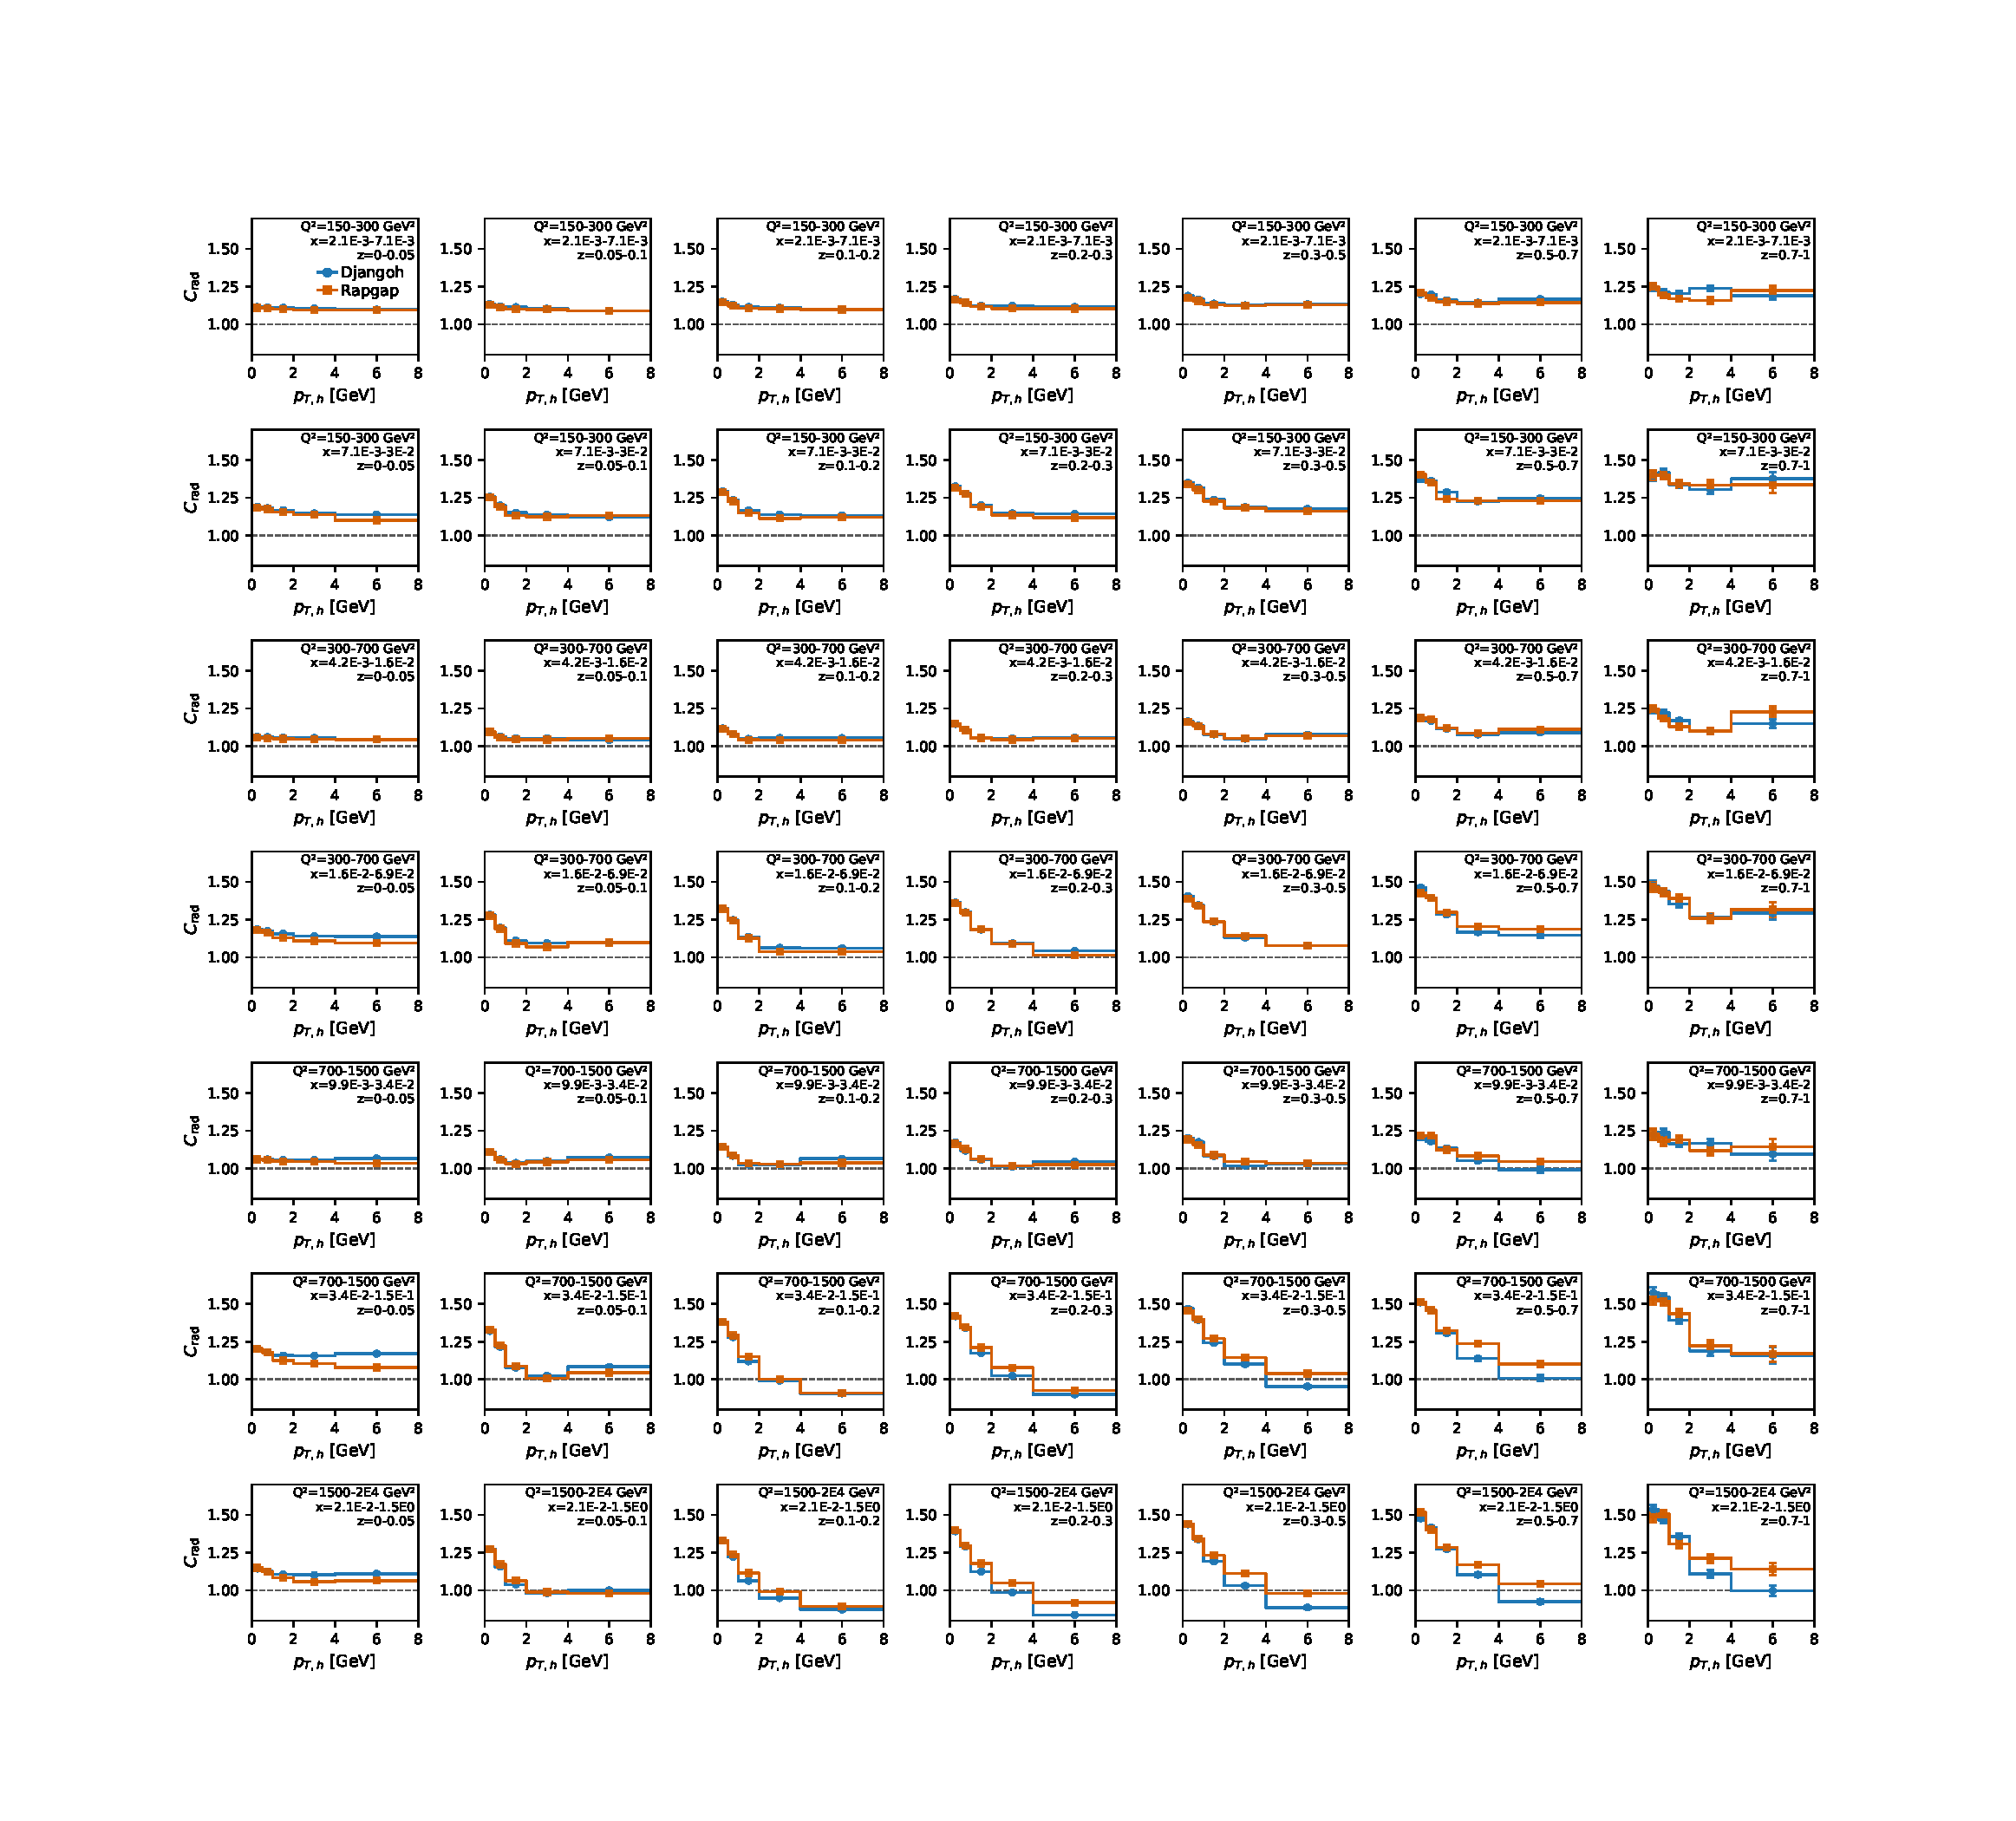
\includegraphics[width=1.05\textwidth,height=0.82\textheight,keepaspectratio]{figures/crad_djangoh14_vs_rapgap31_fLumi_v3_7col_hplus_zoom.pdf}
%   \caption{Comparison of $C_{\mathrm{rad}}=\sigma_{\mathrm{nonrad}}/\sigma_{\mathrm{rad}}$ for DJANGOH14 and RAPGAP31 for $\hplus$.}
%   \label{fig:crad:djangoh-rapgap-flumi-v3-hplus}
% \end{figure}
%
% \begin{figure}[p]
%   \centering
%   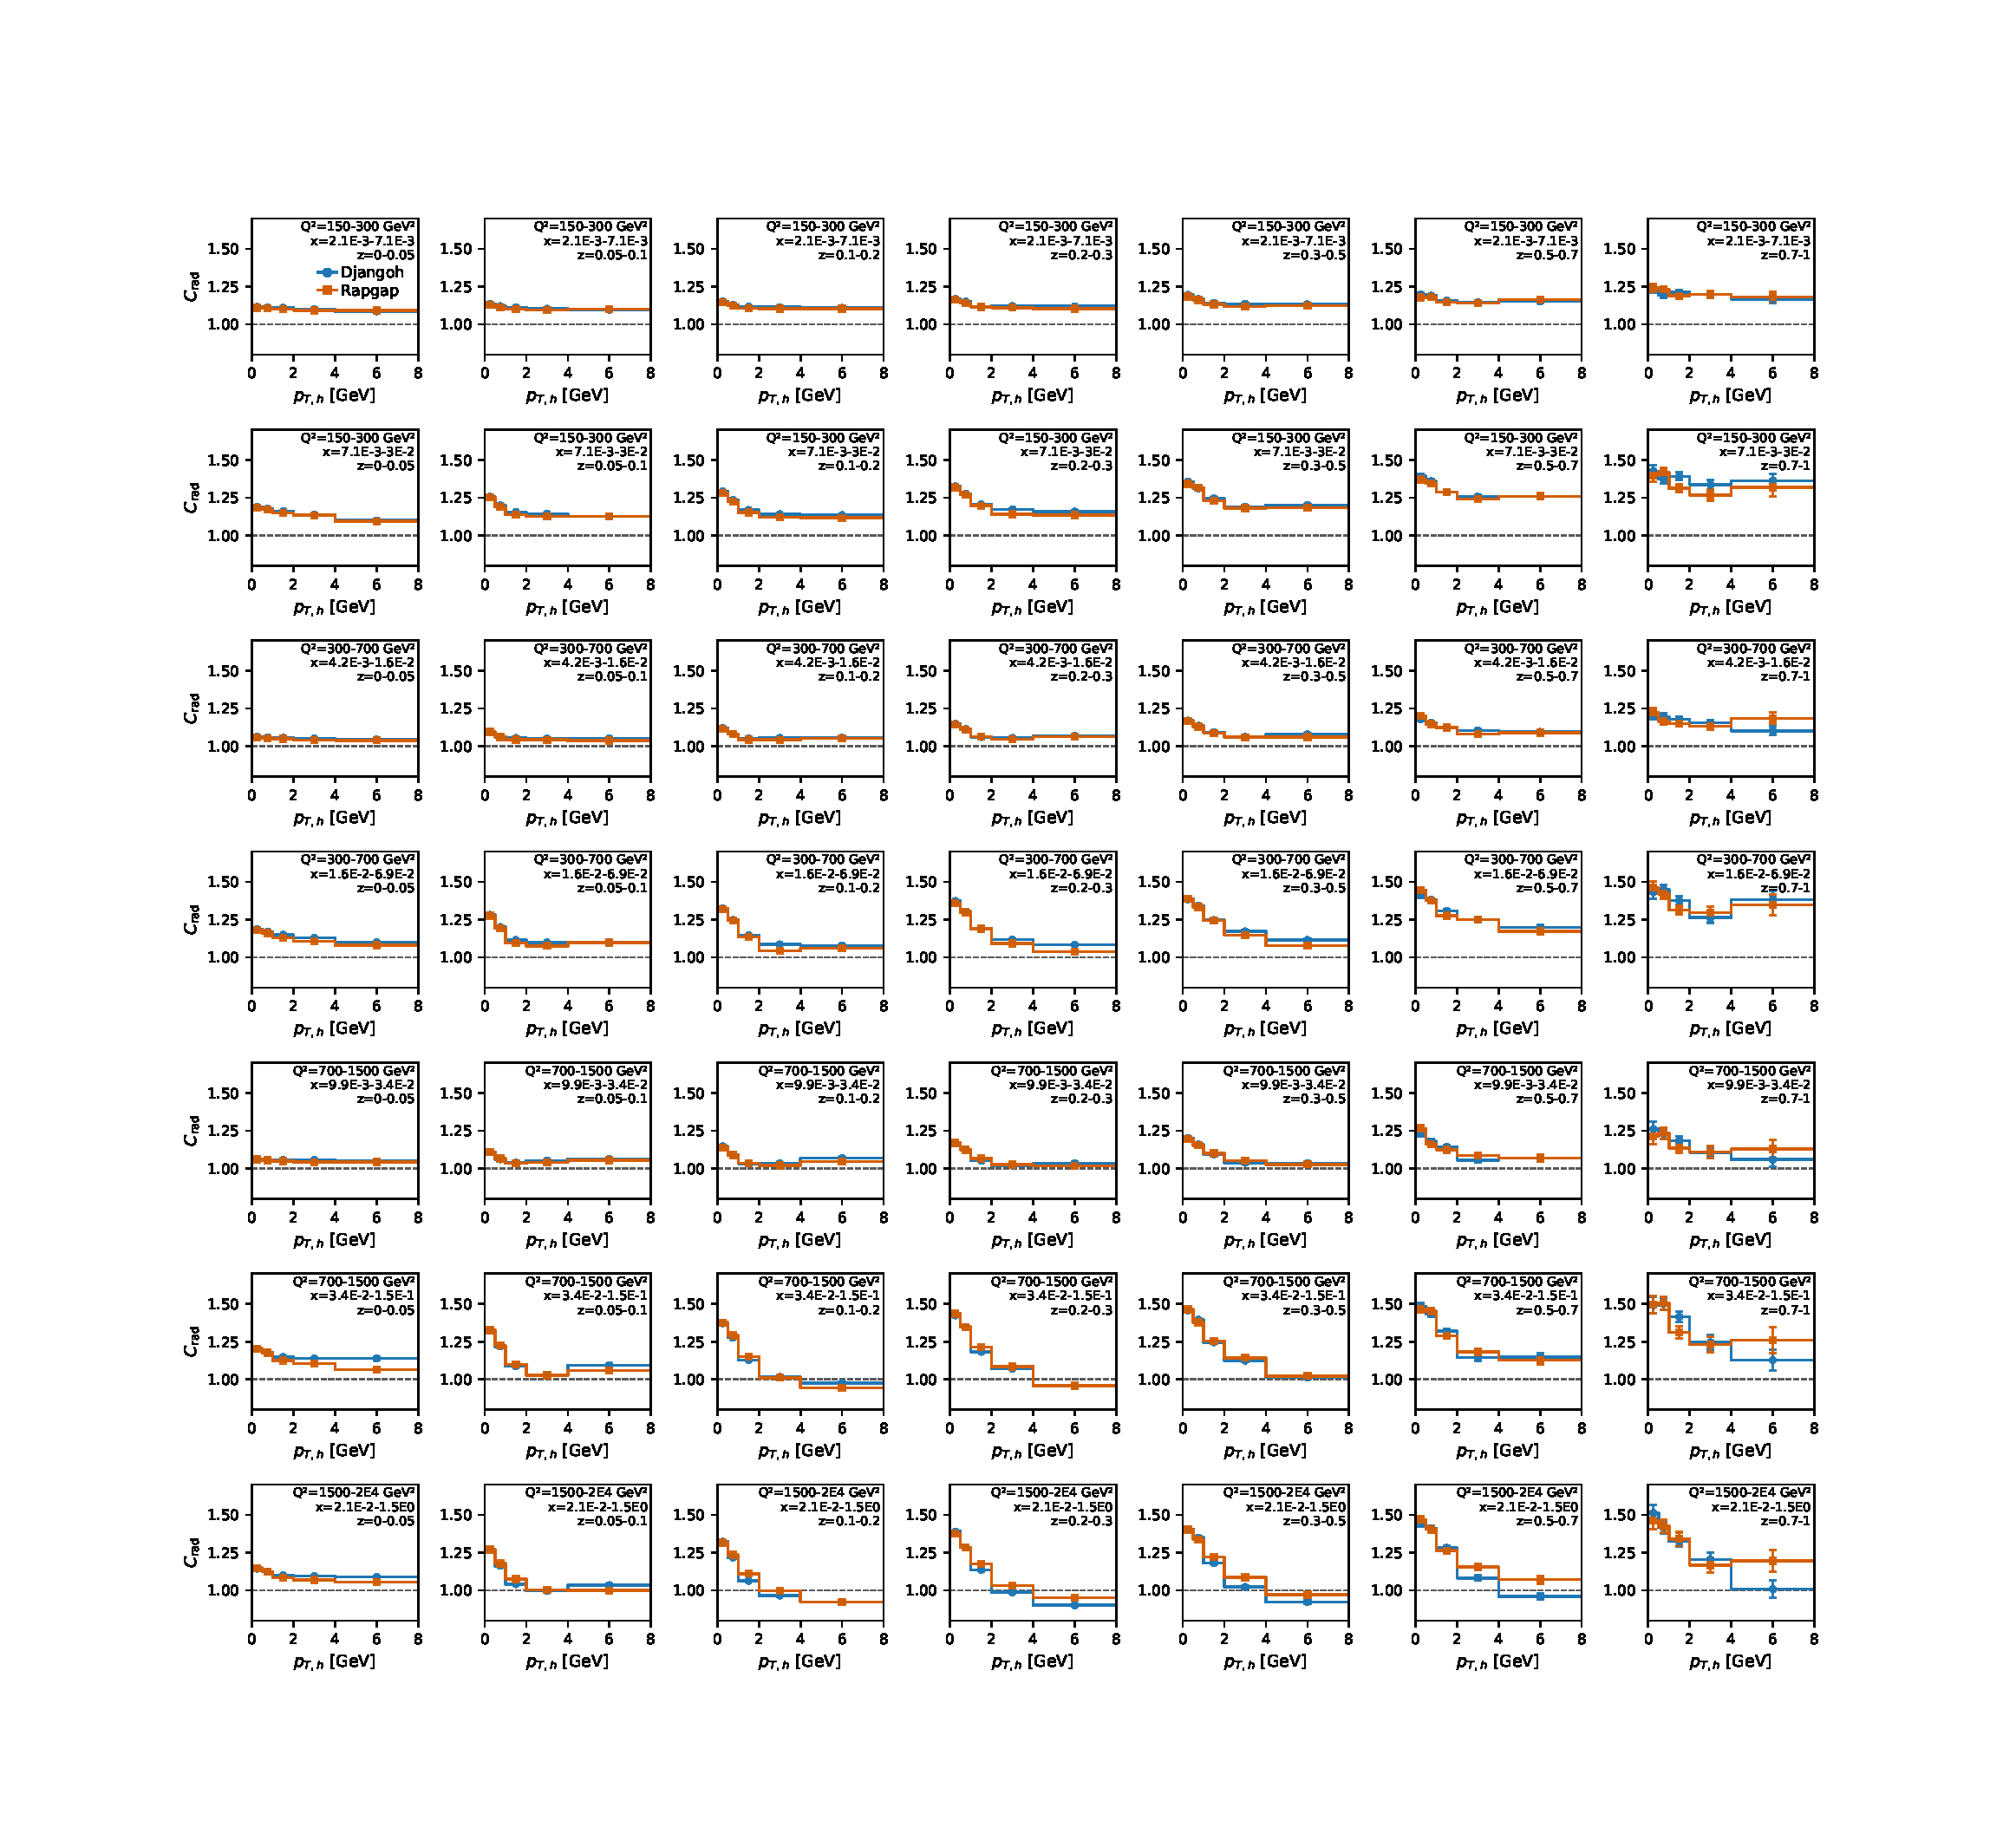
\includegraphics[width=1.05\textwidth,height=0.82\textheight,keepaspectratio]{figures/crad_djangoh14_vs_rapgap31_fLumi_v3_7col_hminus_zoom.pdf}
%   \caption{Comparison of $C_{\mathrm{rad}}=\sigma_{\mathrm{nonrad}}/\sigma_{\mathrm{rad}}$ for DJANGOH14 and RAPGAP31 for $\hminus$.}
%   \label{fig:crad:djangoh-rapgap-flumi-v3-hminus}
% \end{figure}

\subsection{Photon-Only Born Variant $C_{\gamma\mathrm{Born}}$}
\label{sec:radiative_corrections:photon-born-variant}

The Born level used for all results in this note is the Born level of the
full neutral-current process, with both photon and $Z$-boson exchange.
As a diagnostic variant, a second per-bin correction,
$C_{\gamma\mathrm{Born}}$, was derived with the same method, selection,
and binning, mapping the measured cross section instead to a Born level
of pure photon exchange, in which the $Z$-boson contribution is absent.
Its integrated factors are $1.041$ for $\hplus$ and
$1.040$ for $\hminus$; they are smaller than the
$C_{\mathrm{rad}}$ factors because the target level itself is lower, not
because of a different treatment of the photon radiation.  This variant
is a provisional diagnostic product: it is not applied to any result in
this note, and it is derived with DJANGOH only, because no corresponding
photon-only RAPGAP sample exists, so the generator comparison that backs
the main correction is not available for the variant.  The two
corrections map the same measurement to different Born conventions and
must not be composed, averaged, or interchanged; any quoted cross section
must state which of the two Born conventions it uses.

% =====================================================================
% Systematic Uncertainties
% H1 high-Q^2 charged-particle SIDIS analysis note
% =====================================================================
\section{Systematic Uncertainties}
\label{sec:systematics}

The current high-$\Qsq$ analysis release has detector, unfolding,
tracking-efficiency, hadron-azimuth, luminosity, radiative, and
background-subtraction systematic components assembled on the validated
490-row release contract.  It uses the near-electron cone selection with the
detector-interaction-corrected response and the pre-unfold subtraction of the
electron, V0, and low-$\Qsq$ background templates; the iterative Bayesian
unfolding of the subtracted data vector is the single denominator for every
relative component.  The frozen 2026-10-19 edition is
\path{systematics_bgsub_env100_21comp_2026-10-19/} under
\path{H1ChargedSidis_HighQ2/output_v6/central/data_release/}.  It inventories
21 columns: 20 active quadrature terms and the retired audit-only
\texttt{bgsub\_stat\_rel} column.  The active total,
\texttt{total\_with\_env100\_rel}, has medians of $7.320288331169215\%$ for
$\hplus$ and $7.637124635311324\%$ for $\hminus$, maxima of
$73.65119705575378\%$ and $88.43670499154085\%$, and no bins above $100\%$.
The frozen input, median, integrated-effect, and no-bin-above-$100\%$ gates
all passed.  This edition had superseded the 2026-10-17 19-component
clean-denominator budget as the quoted systematic; the latter is retained as
historical provenance.  Both frozen editions were computed on the central
values that the 2026-10-20 OPT-A baseline promotion superseded
(Sec.~\ref{sec:results:z005-release}): they are superseded as a quoting
basis, are retained unchanged as provenance, and the budget is being
regenerated on the OPT-A nominal
(Sec.~\ref{sec:syst:budget-regeneration}); until the regenerated budget
passes review, no per-bin uncertainty and no uncertainty total is final.
Global covariance matrices constructed from the frozen 2026-10-19 budget are
described in Sec.~\ref{sec:syst:global-covariance}.  The
radiative correction $C_{\mathrm{rad}}$ is applied to the cross section at
Born level, with its uncertainty carried as the two systematic components
described in Sec.~\ref{sec:radiative_corrections} and listed in
Table~\ref{tab:syst:z005-components}.  The remaining open item for the
radiative correction is its application at the multiplicity level.

\subsection{Budget Regeneration on the OPT-A Nominal}
\label{sec:syst:budget-regeneration}

The systematic budget is being regenerated on the OPT-A nominal central
values (Sec.~\ref{sec:results:z005-release}).  Until the regenerated budget
passes review, no per-bin uncertainty and no uncertainty total of the frozen
editions may be quoted as final.  The regeneration and its companion open
items are:
\begin{itemize}
  \item the re-derivation of the affected components on the OPT-A nominal,
        together with the fix of the detector-interaction double count in
        the twenty-active-term total: the removal term enters the quadrature
        sum twice, an inflation proven exactly in three independent
        re-derivations, of at most about $1.71\times10^{-4}$ relative and
        never deflating, so the frozen totals are strictly conservative;
  \item the per-bin treatment of the 56 published bins whose OPT-A Born
        shift exceeds the per-bin background-envelope component of the
        frozen budget (largest ratio 2.58; no bin exceeds the frozen
        edition totals, with maximum ratios 0.86 and 0.70 against the
        nineteen- and twenty-active-term editions, a statement robust to
        the double-count fix), and the assignment of a systematic home to
        the residual straddle-rate model dependence---the residual mismatch
        of the per-cell straddle rates between simulation and data, bounded
        by the same straddle logic;
  \item the form of the declared $z$-bin-row shift convention
        (Sec.~\ref{sec:unfolding:truth-contract}): caveat only, or a budget
        component; if a component is chosen, the only sound derivation is a
        self-consistent scheme pair---a response variant with the rad-safe
        generator $z$ together with a co-derived correction on the same
        basis---and never a rad-safe-$z$ response combined with the current
        correction table, which would double-count the $z$ migration;
  \item the reconstruction of the frozen-edition budget builder, whose
        provenance could not be located; the acceptance condition is the
        exact reproduction of the nineteen-component total on the three
        empty-subtracted-data bins (positive charge, bins 109 and 179;
        negative charge, bin 240);
  \item the missing HFS--$E-p_z$ systematic channel: the
        hadronic-final-state shifts leave $E-p_z$ bit-identical, so the
        quoted HFS-leg errors do not cover the $E-p_z>45~\GeV$ requirement;
  \item the re-basing of the fractional covariance product of
        Sec.~\ref{sec:syst:global-covariance} to the OPT-A nominal;
  \item the re-pointing and repair of the registered canonical plotting
        chain, whose script audit failed with 24 defects and whose
        registered Born plotter still reads a superseded release, and the
        remaining publication-facing canonical plot categories, which
        depend on the regenerated budget.
\end{itemize}

\subsection{List of Systematics}
\label{sec:syst:z005-components}

Table~\ref{tab:syst:z005-components} lists the components of the total
uncertainty as combined in the frozen budget editions
(Sec.~\ref{sec:syst:budget-regeneration}). The HFS and electron sources of uncertainty are calculated using the standard H1CalcSystematic framework.

\begin{table}[h]
\centering
\small
\begin{tabular}{p{4.5cm}p{10.3cm}}
\toprule
Component & Treatment \\
\midrule
IBU statistical uncertainty & $\sigma$ of 1000 Poisson-only toy replicas on the subtracted data vector \\
IBU model uncertainty & Difference in unfolded data with different model migration matrices \\
IBU regularization uncertainty & $\pm1$ iteration around nominal $N_{\mathrm{iter}}=4$ \\
Hadron-azimuth prior & Flat-$\phih$ IBU prior; half the larger generator deviation \\
Scattered-electron energy & 1\% shift of $E_{e'}$ \\
Scattered-electron polar angle & Shift of $\theta_{e'}$ by $1~\mathrm{mrad}$\\
Tracking efficiency & $-0.5\%$ tracking-efficiency shift\\
HFS JES & Shift of JES by 2\% \\
HFS RCES & Shift of RCES by 2\%\\
HFS polar angle & Shift of HFS $\theta$ by 1 mrad \\
Radiative generator difference & DJANGOH vs RAPGAP, median $0.5844/0.5804\%$ ($\hplus/\hminus$) \\
Radiative correction statistics & Statistical uncertainty, median $0.4272/0.4429\%$ ($\hplus/\hminus$) \\
Detector-integration removal & Removal-increment isolation of the detector-interaction reroute on the subtracted chain; median $0.0299/0.0287\%$ ($\hplus/\hminus$) \\
Fake-column MC statistics & Cone fake-column $\sigma(f_i)$ propagated through the unfolding Jacobian on the subtracted data vector; median $0.3437/0.3494\%$ ($\hplus/\hminus$) \\
Background-subtraction model & V0 and electron generator half-spreads in quadrature with a $\pm30\%$ low-$\Qsq$ scale term \\
Background-subtraction stage & Pre-versus-post-unfold stage difference measured on the cone chain \\
Background-subtraction fake fraction & Fake-fraction common-model dependence $|1-r_{\min}|\,f_i$ with the proxy $r_{\min}=0.9817$ (NucliaWeight caveat) \\
Background-subtraction envelope & Fully correlated $\pm100\%$ normalization envelope on $(e_{\mathrm{avg}}+V0_{\mathrm{avg}})/\mathrm{data}_{\mathrm{sub}}'$; \texttt{bgsub\_stat\_rel} is retained audit-only and excluded from the total \\
Luminosity & flat $2.7\%$ \\
\bottomrule
\end{tabular}
\caption{The systematic-uncertainty components of the frozen budget editions and how they are calculated.  The detector-integration removal entry comprises two terms, its model and statistical parts, so the inventory holds twenty active quadrature terms in total.  The audit-only retired \texttt{bgsub\_stat\_rel} column is not included in the quadrature sum.}
\label{tab:syst:z005-components}
\end{table}

The five detector components (scattered-electron energy and polar angle, and
HFS JES, RCES, and polar angle) are full-chain single-sided variations: the
shift is applied at the reconstructed electron or HFS and propagated through
the shifted-chain response and unfolding, with RAPGAP31 governing and absolute
single-sided differences taken; on the current background-subtracted release
the background templates are subtracted from each shifted data vector as
well.  For the
scattered-electron energy component
the leg with the larger robust median is used per charge, the leg-level
envelope; the HFS legs are produced in the plus direction only and their sign
symmetry is assumed, a deferred follow-up.  The tracking-efficiency component
remains a data-side conservative shift, with medians $0.5132\%$
($\hplus$) and $0.5211\%$ ($\hminus$) on the background-subtracted denominator.  The
two radiative components are unchanged by the detector-interaction,
cone-baseline, and background-subtraction promotions of the observable basis,
carried bit-identically.

The shifts applied to the HFS primarily enter the measurement through the calculation of $E-P_z$. They do not affect the tracks.

The electron and V0 background templates used in the pre-unfold subtraction
are MC-derived and their normalization
could not be measured by the dedicated control-region fits: in the
$|\mathrm{DcaPrime}|>0.25~\mathrm{cm}$ tail, the two-class model is
unidentifiable, with the V0 normalization at its lower bound and the electron
normalization drifting to $2.5$--$3.5$ in the failed groups, while five of the
eight fits fail and the accepted groups remain compatible with unity.  The
nominal subtraction corresponds to $7.28\%$ of the cone data vector, composed
of $3.85\%$ electron and $3.42\%$ V0 content; it is therefore assigned the
fully correlated $\pm100\%$ envelope
$\texttt{bgsub\_env100\_rel}=(e_{\mathrm{avg}}+V0_{\mathrm{avg}})/\mathrm{data}_{\mathrm{sub}}'$
rather than using the retired template-statistics term.  The tightened-chain
check, in which $|\mathrm{DcaPrime}|<0.3~\mathrm{cm}$ is propagated through
data, response, templates, and unfolding, finds 87 shifts above $3\sigma$
where 1.21 are expected from statistical fluctuations; its integrated Born
changes, $-2.37\%$ ($\hplus$) and $-1.40\%$ ($\hminus$), require correlated
content uncertainties of $30.7\%$ and $17.6\%$, respectively.  In the
per-bin requirement study, 23 significant shifts require more than $30\%$,
10 require more than $50\%$, and the largest requirement is $97\%$; every
significant shift is contained by the $\pm100\%$ envelope.  The earlier DCA
scan is a diagnostic-only far-tail study, not a component of the quoted
budget; crediting even its one-sided tightening does not remove the need for
the envelope.  The DCA removal itself rejects $200\%$--$300\%$ more tracks
than the associated template background, so the residual tail excess is of
unknown composition and can include displaced signal.  The residual risk is
therefore recorded rather than interpreted as a background measurement: the
coherent envelope is $7.715610295533167\%$ ($\hplus$) and
$7.973016448067494\%$ ($\hminus$), corresponding at Born level to
$\pm0.9256076766034321~\mathrm{nb}$ and
$\pm0.929969093275612~\mathrm{nb}$ on the $11.996558161307064~\mathrm{nb}$
and $11.663955534683723~\mathrm{nb}$ integrated cross sections, respectively.
The fully correlated treatment is retained across bins and charges.  It does
not remove the standing caveats on the low-$\Qsq$ template scale, the
NucliaWeight fake-fraction proxy, or the blocked DIFFVM and photoproduction
register rows; the near-electron cone remains motivated by the previous H1
charged-particle measurement~\cite{H1:2013qsm}.

\subsection{Per-Source Fractional-Uncertainties}
\label{sec:syst:source-plots}

Figures~\ref{fig:syst:sources-hplus-env100-fullrange}--\ref{fig:syst:sources-hminus-env100-midrange}
display the per-source fractional systematic uncertainties and their quadrature
sum for $\hplus$ and $\hminus$ in percent units.  The display shows all 21
inventory components, the active total, and the superseded 19-component total
as a dashed reference.  The active total is
\texttt{total\_with\_env100\_rel}, with medians $7.320288331169215\%$ for
$\hplus$ and $7.637124635311324\%$ for $\hminus$.  The retired audit-only
\texttt{bgsub\_stat\_rel}
column is not plotted or included in this total.

The three fixed vertical ranges provide the full 0--100\% range, the 0--15\%
zoom, and the intermediate 0--50\% range.  The figures are dated
candidate renderings of the frozen 2026-10-19 budget, which is superseded as
a quoting basis (Sec.~\ref{sec:syst:budget-regeneration}); the
publication-version plotting script for these panels is not yet registered.

\begin{figure}[p]
  \centering
  \begin{subfigure}[t]{0.98\textwidth}
    \centering
    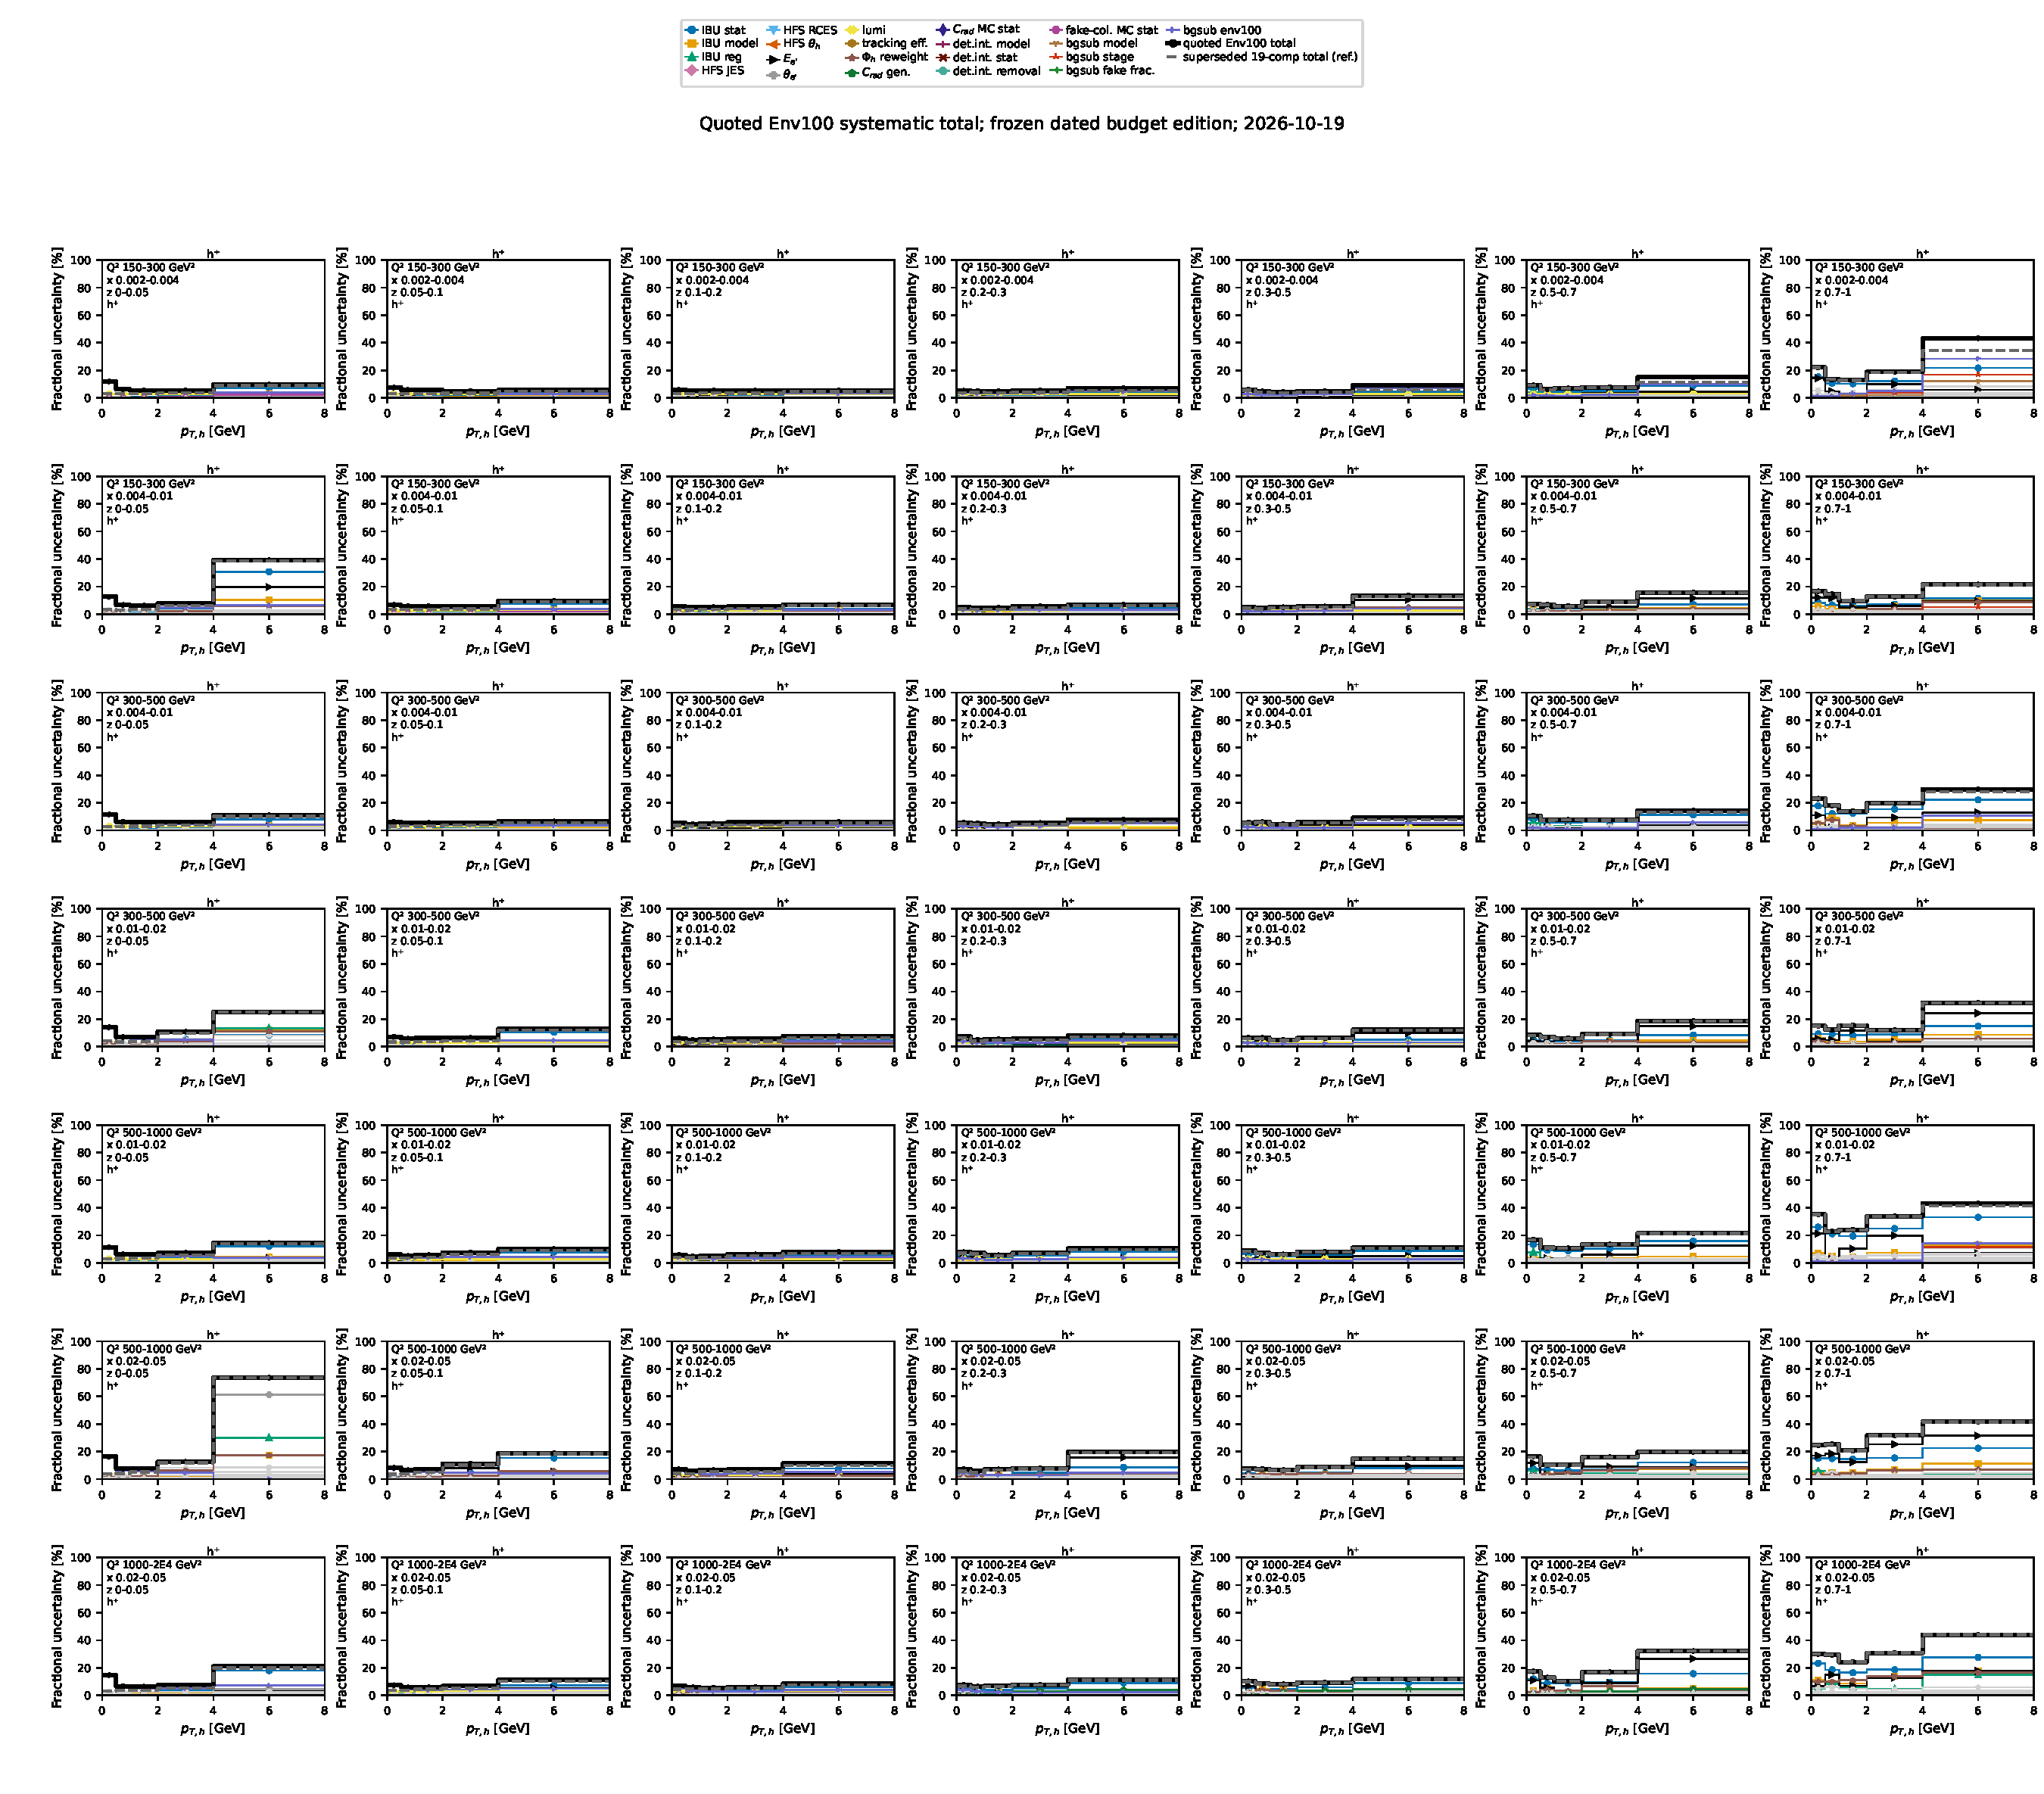
\includegraphics[width=\textwidth,height=0.38\textheight,keepaspectratio]{figures/fig_syst_uncertainty_sources_hplus_env100_ylim100.pdf}
    \caption{Full 0--100\% range.}
  \end{subfigure}
  \par\medskip
  \begin{subfigure}[t]{0.98\textwidth}
    \centering
    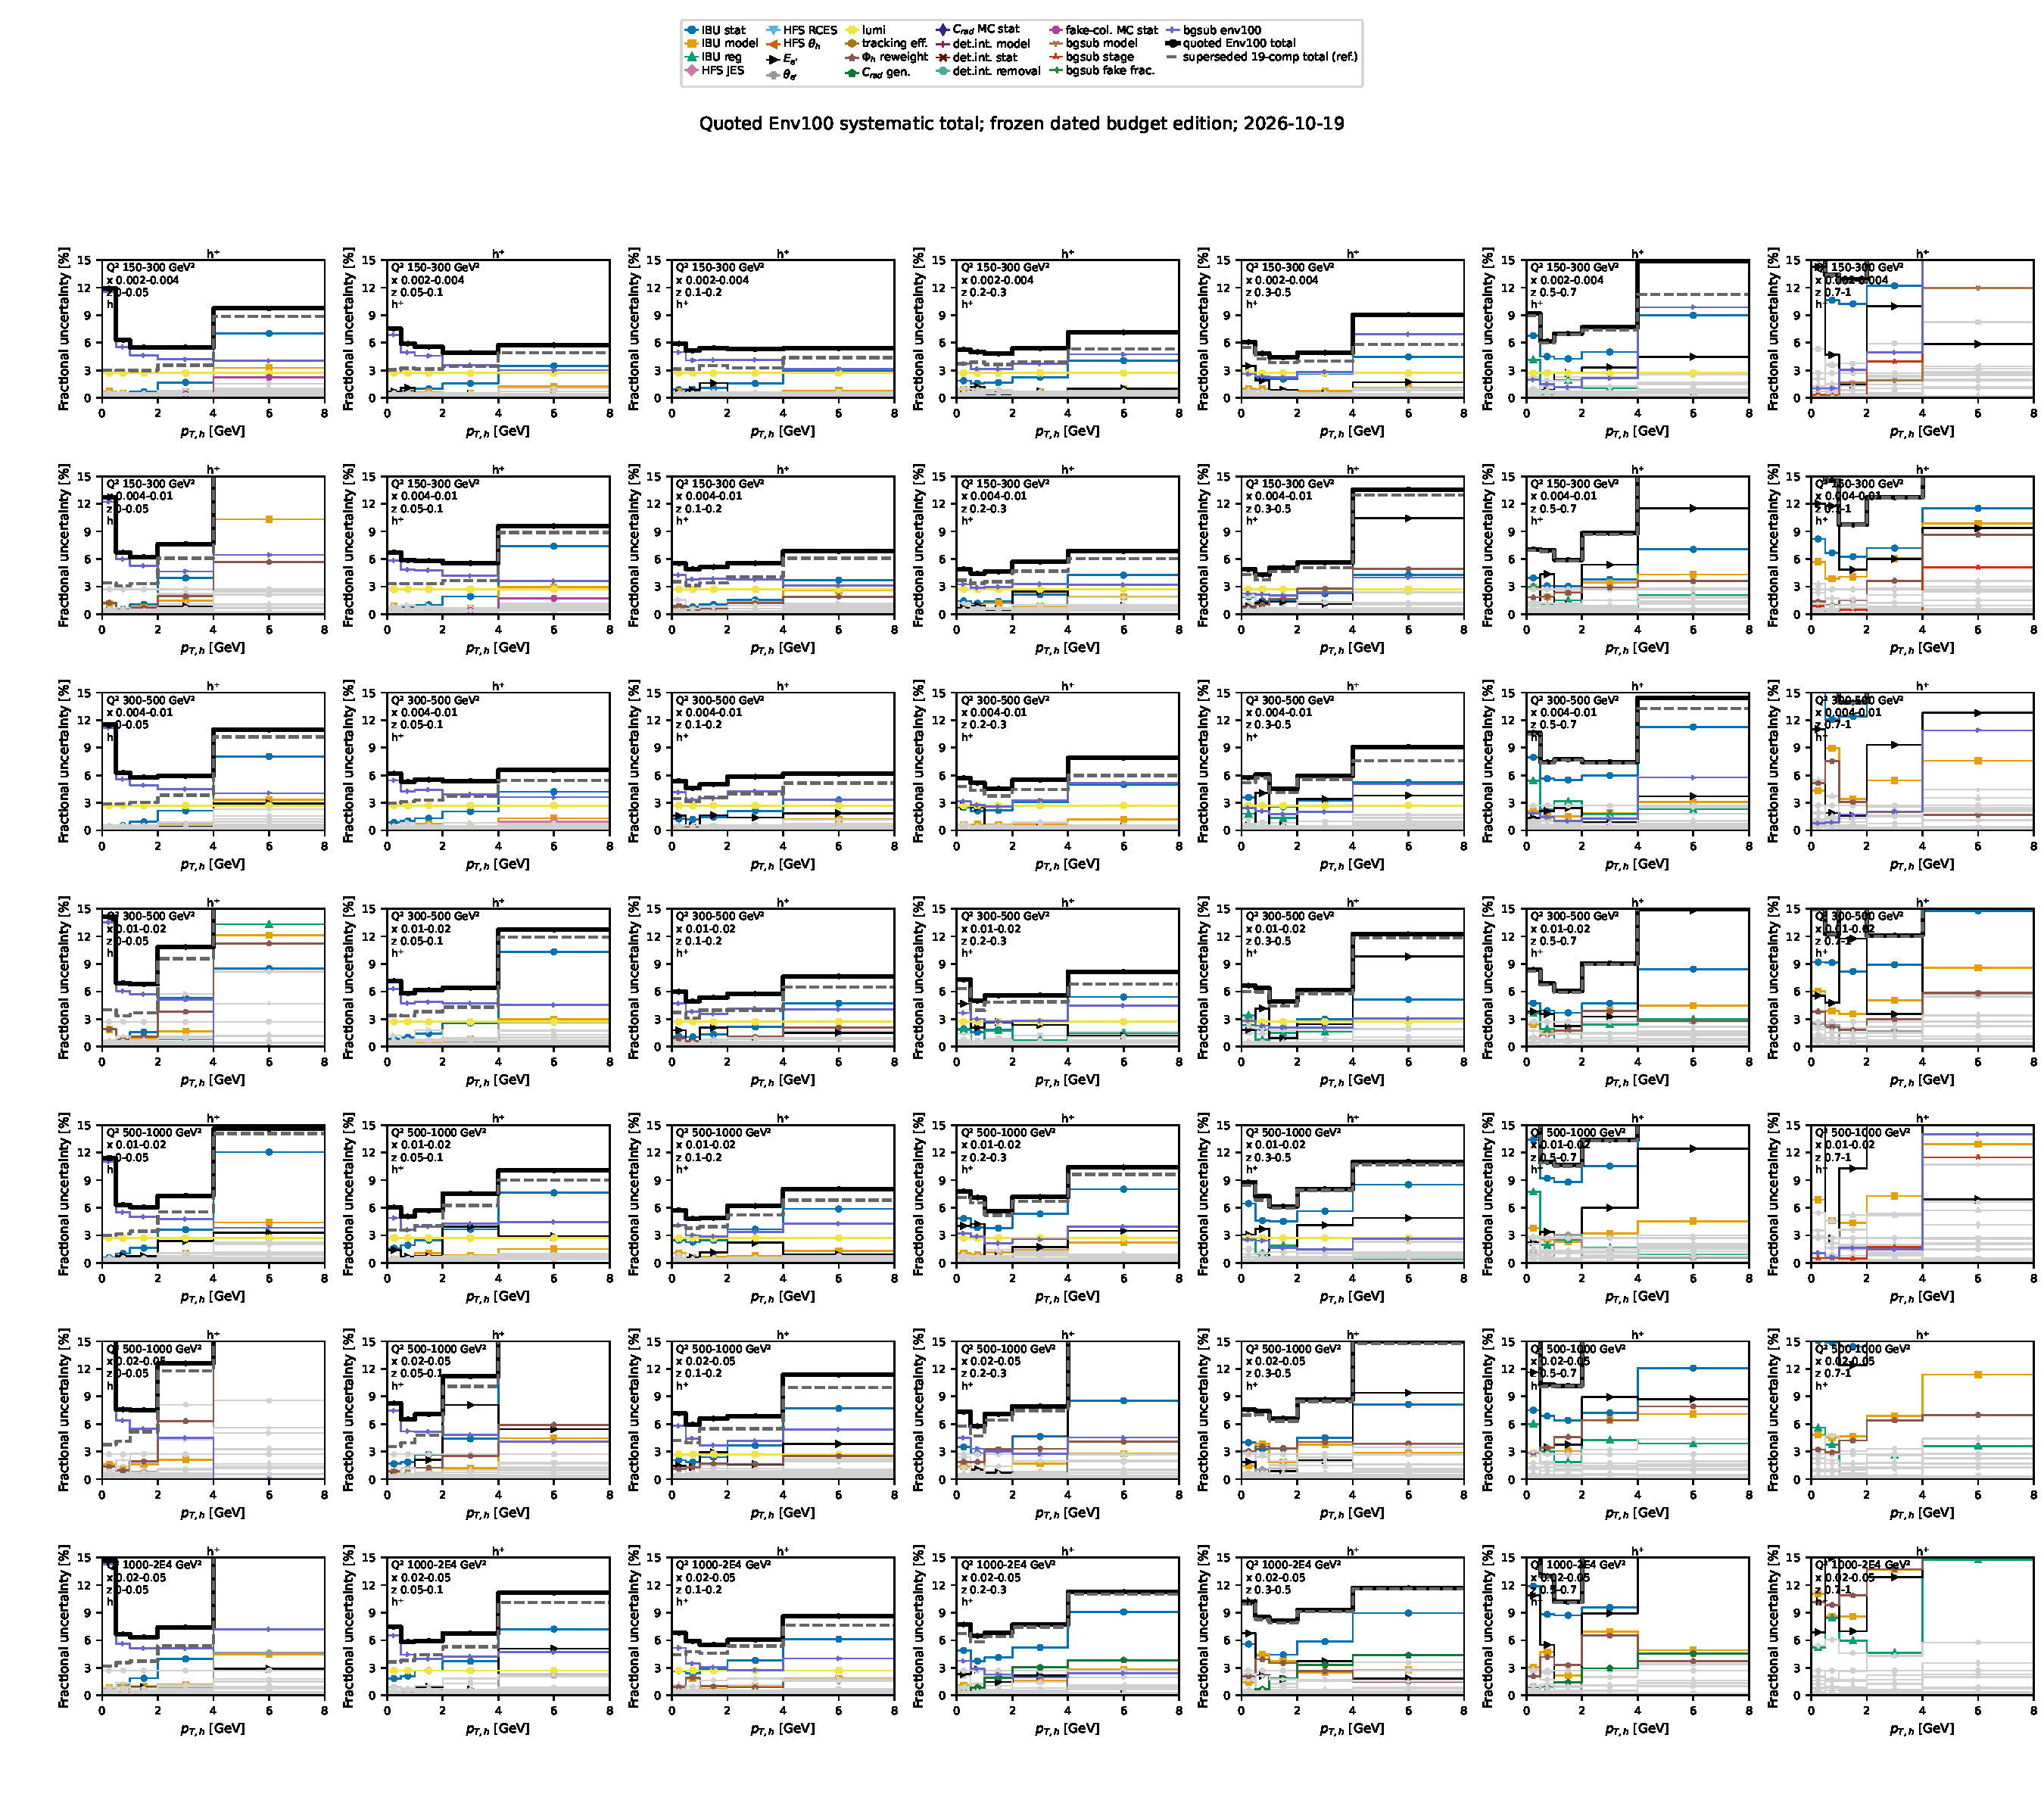
\includegraphics[width=\textwidth,height=0.38\textheight,keepaspectratio]{figures/fig_syst_uncertainty_sources_hplus_env100_ylim015.pdf}
    \caption{0--15\% zoom.}
  \end{subfigure}
  \caption{Per-source fractional systematic uncertainties for $\hplus$ versus
  $\pTh$ on the frozen 2026-10-19 uncertainty basis, shown in percent units.}
  \label{fig:syst:sources-hplus-env100-fullrange}
\end{figure}

\begin{figure}[p]
  \centering
  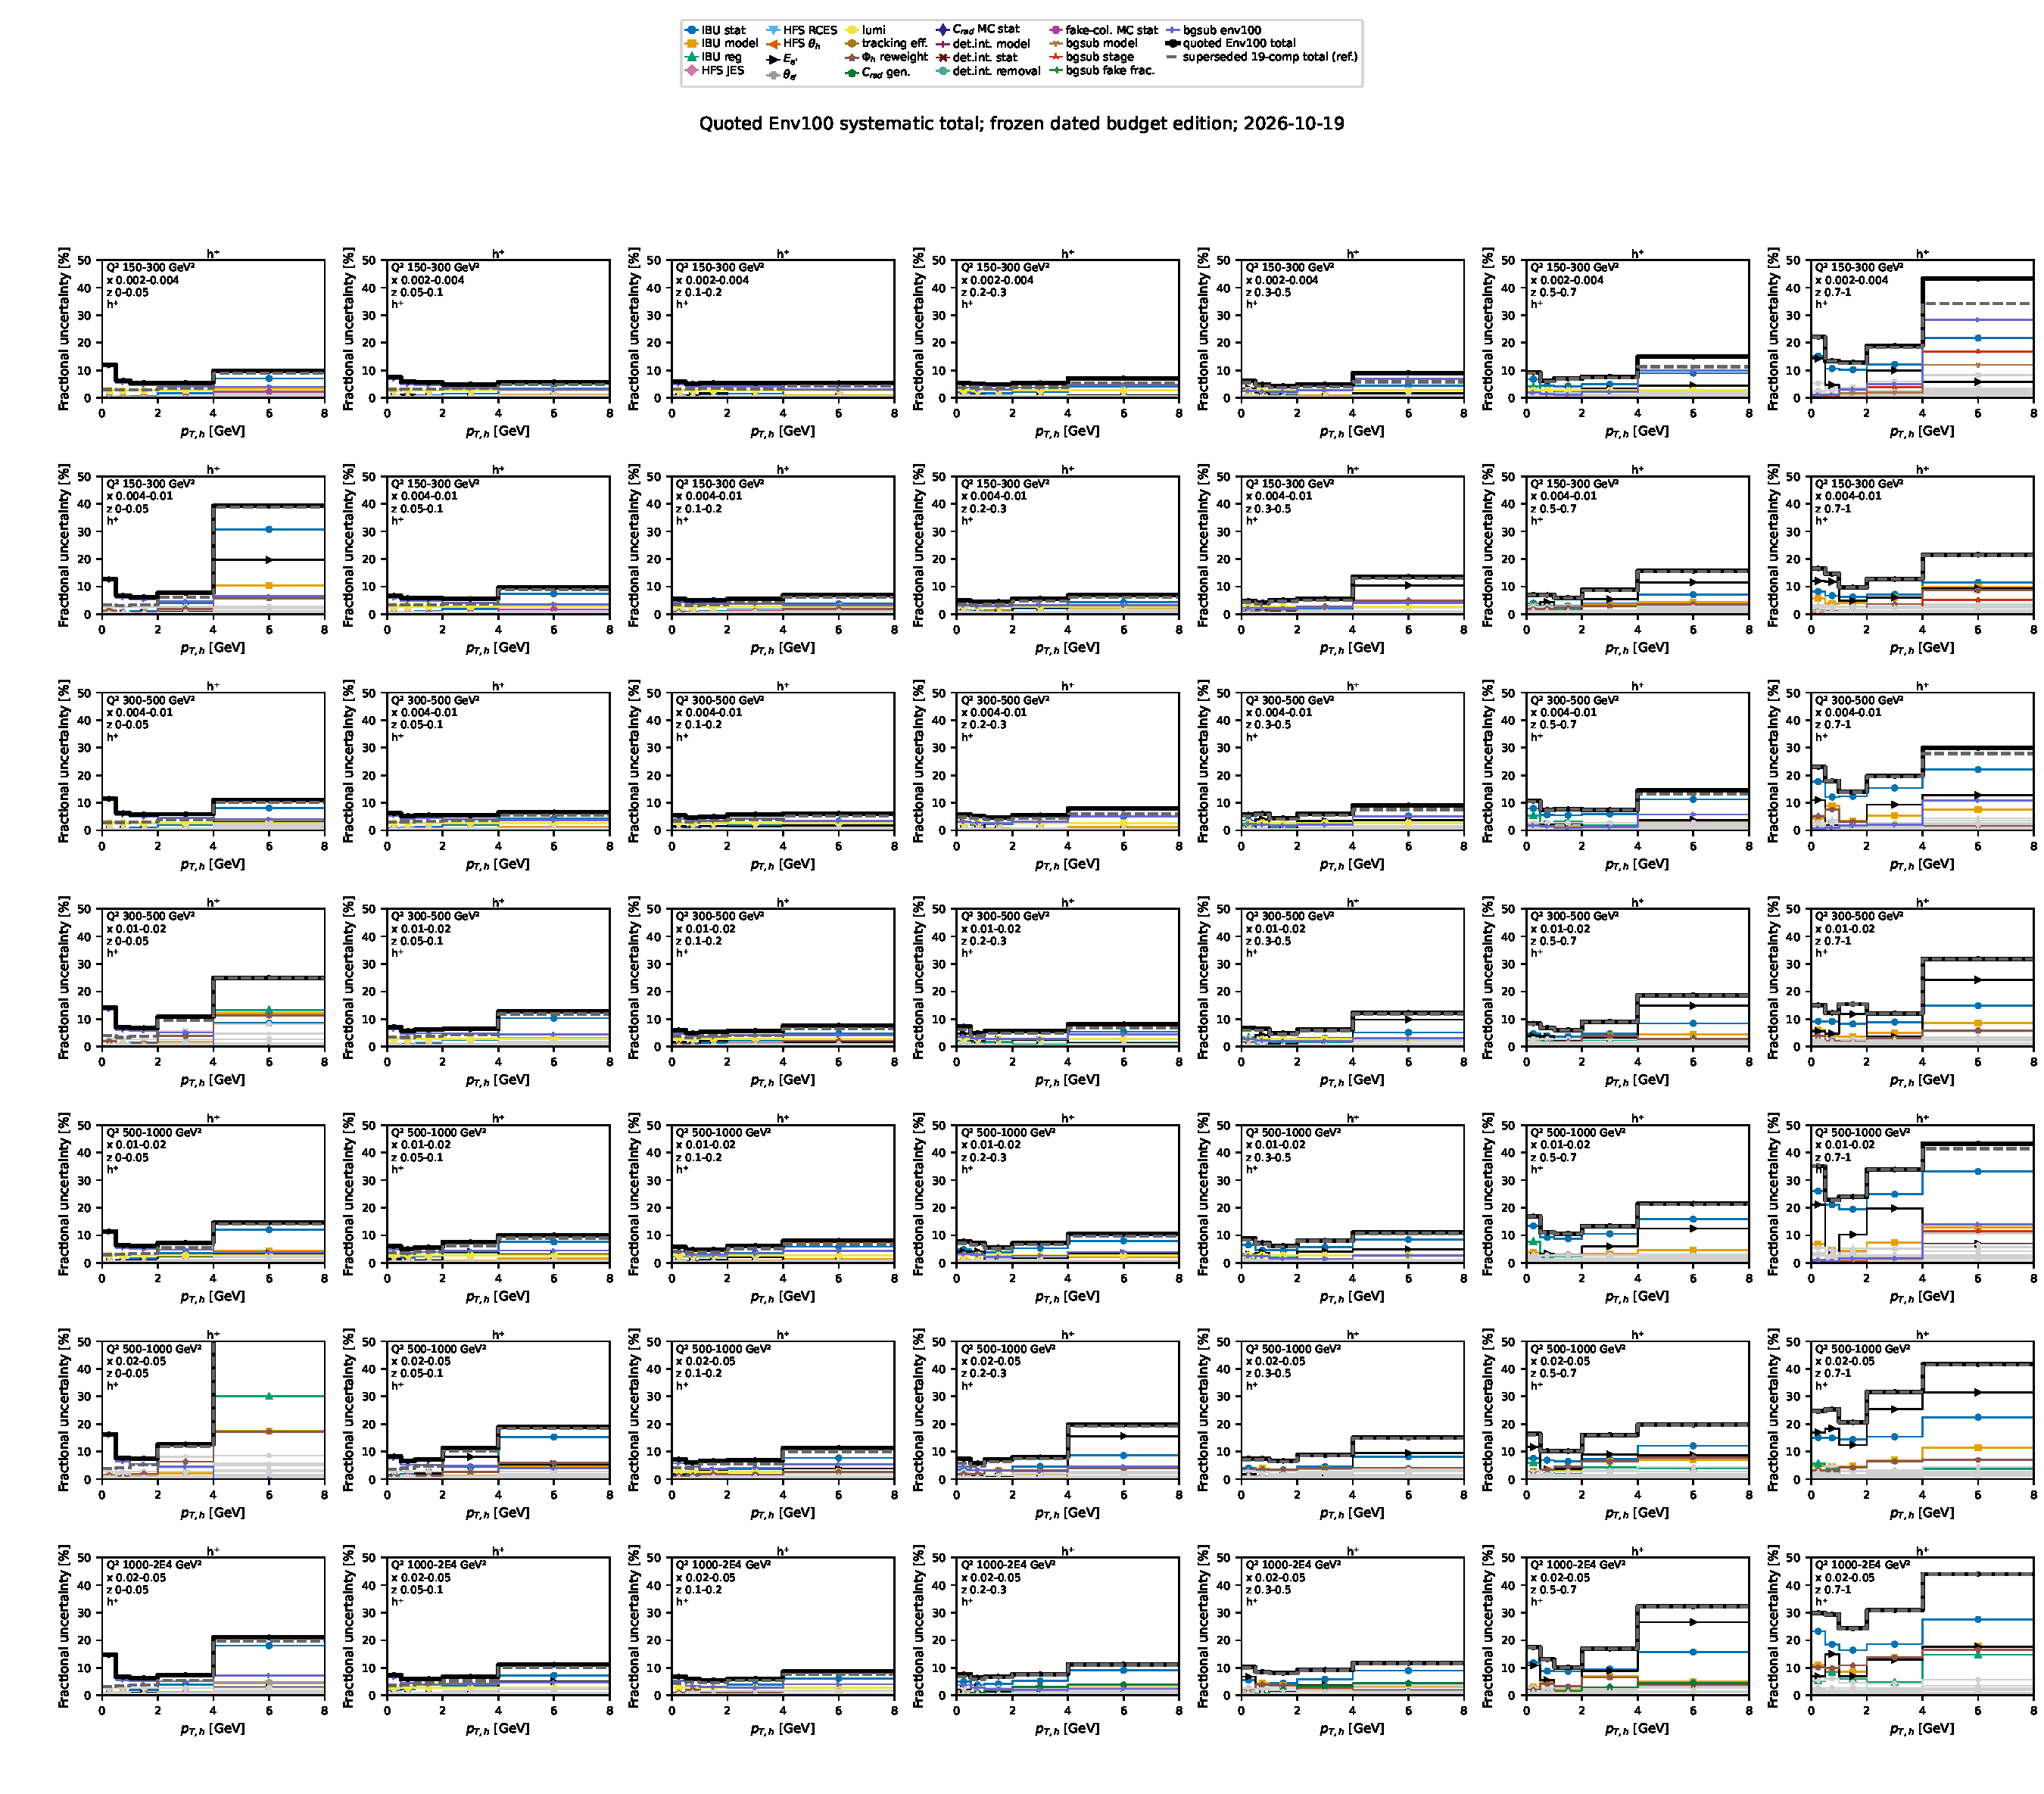
\includegraphics[width=0.98\textwidth,height=0.82\textheight,keepaspectratio]{figures/fig_syst_uncertainty_sources_hplus_env100_ylim050.pdf}
  \caption{Per-source fractional systematic uncertainties for $\hplus$ versus
  $\pTh$ on the frozen 2026-10-19 uncertainty basis, shown in percent units with a fixed
  0--50\% vertical range.}
  \label{fig:syst:sources-hplus-env100-midrange}
\end{figure}

\begin{figure}[p]
  \centering
  \begin{subfigure}[t]{0.98\textwidth}
    \centering
    \includegraphics[page=2,width=\textwidth,height=0.38\textheight,keepaspectratio]{figures/fig_syst_uncertainty_sources_hminus_env100_ylim100.pdf}
    \caption{Full 0--100\% range.}
  \end{subfigure}
  \par\medskip
  \begin{subfigure}[t]{0.98\textwidth}
    \centering
    \includegraphics[page=2,width=\textwidth,height=0.38\textheight,keepaspectratio]{figures/fig_syst_uncertainty_sources_hminus_env100_ylim015.pdf}
    \caption{0--15\% zoom.}
  \end{subfigure}
  \caption{Per-source fractional systematic uncertainties for $\hminus$ versus
  $\pTh$ on the frozen 2026-10-19 uncertainty basis, shown in percent units.}
  \label{fig:syst:sources-hminus-env100-fullrange}
\end{figure}

\begin{figure}[p]
  \centering
  \includegraphics[page=2,width=0.98\textwidth,height=0.82\textheight,keepaspectratio]{figures/fig_syst_uncertainty_sources_hminus_env100_ylim050.pdf}
  \caption{Per-source fractional systematic uncertainties for $\hminus$ versus
  $\pTh$ on the frozen 2026-10-19 uncertainty basis, shown in percent units with a fixed
  0--50\% vertical range.}
  \label{fig:syst:sources-hminus-env100-midrange}
\end{figure}

\subsection{Fractional Covariance Matrices}
\label{sec:syst:global-covariance}

The frozen 2026-10-19 uncertainty product provides fractional cross-section
covariance matrices on the 245 published bins per charge.  The matrices are
constructed for the current observable basis, with the near-electron cone
selection, the electron, V0, and low-$\Qsq$ backgrounds subtracted from the
data before unfolding, and the iterative Bayesian unfolding result taken on
the subtracted data vector.  They
encode the 20 active terms of the current budget: \texttt{ibu\_stat\_rel}
and 19 systematic terms.  The retired \texttt{bgsub\_stat\_rel} column is not
included.

The correlation model is deliberately limited to validated declarations.
The luminosity and \texttt{bgsub\_env100\_rel} terms are fully correlated
across all bins and between charges.  All other components are represented
as bin-diagonal because no validated inter-bin correlation model is available
for them in this edition.  Consequently, the cross-charge covariance contains
only the luminosity and background-envelope rank-one terms; the IBU
statistical term is
stored separately as a diagonal fractional covariance.  The diagonal of the
combined covariance reproduces \texttt{total\_with\_env100\_rel}$^2$, with
maximum relative deviations of $5.431899438732146\times10^{-15}$ for
$\hplus$ and $6.403330938130179\times10^{-15}$ for $\hminus$.

The matrices are symmetric and positive definite in each charge block: the
minimum fractional eigenvalues are $7.681667696346608\times10^{-5}$ for
$\hplus$ and $8.165371868314269\times10^{-5}$ for $\hminus$.  The
cross-charge block is symmetric.  These matrices provide the declared
fractional-covariance model only; they do not supply a new response-MC
statistical covariance or a correlation model for the bin-diagonal
components.  Any use must state the Born-versus-raw level of the nominal
cross section used to convert fractional covariance to cross-section units.

The product is retained at
\path{/data/dust/group/h1/klesthen/BaryonAsym/H1ChargedSidis_HighQ2/output_v6/central/data_release/systematics_bgsub_env100_21comp_2026-10-19/covariance/}.
It contains the per-charge and cross-charge fractional systematic covariance
matrices, the separately stored IBU-statistical matrices, a total-correlation
rendering, and the gate record.  The gate record and release status report
all covariance/correlation checks as passed.  The package was constructed on
the superseded central values and is pending re-basing to the OPT-A nominal
(Sec.~\ref{sec:syst:budget-regeneration}); its diagonals also carry the
conservative detector-interaction double count of the frozen total.

\subsection{Detector and Track-Selection Robustness Cross-Checks}
\label{sec:syst:cut-variations}

In addition to the systematic components included in the nominal budget, several
detector and track-selection variants have been performed as robustness checks
rather than central results. Ideally, the measurement would be insensitive to
small changes in detector-level cuts. We study the effect of varying the $E-p_z$
cut, the minimum lab-frame $p_T$, the $\eta$ cut, and the cut on the distance of
closest approach, generating a new migration matrix with these reconstructed-level
cuts and then repeating the IBU unfolding procedure on the data. The results are
shown as the ratio of the unfolded cross section with the nominal cut to the
measured cross section with the varied cut for all bins in
\cref{fig:syst:cutvar-empz25,fig:syst:cutvar-labpt,fig:syst:cutvar-eta,fig:syst:cutvar-dca1,fig:syst:cutvar-dca3}. The uncertainties on the points in these figures show the model, statistical, and regularization uncertainties of the IBU unfolding.
These variants were produced before the coherent-prior re-release and the
subsequent detector-interaction and cone-baseline promotions, on an earlier
release lineage; they are retained as robustness checks of the cut scheme and
have not been repeated on the current cone-based release.

The loosening or tightening of the DCA cut is observed to have essentially no impact on the result. The lab $p_T$ cut has a 3-4\% effect on the lowest $\pTh$ bins, with one bin (with huge statistical uncertainties) exhibiting a 10\% shift. The lab $\eta$ cut has the most significant impact, due to the fact that it removes a much larger number of particles. A few bins are reduced to having low statistics after imposing the $|\eta|<1.4$ cut, so large fluctuations in the unfolded data in these bins can be expected. As before, these bins generally already have a large systematic and statistical uncertainty. Even in the worse case, all bins lie within 2 sigma of the unvaried results.


\begin{table}[h]
\centering
\small
\begin{tabular}{p{2.5cm}p{4.7cm}p{2.1cm}p{2.1cm}p{2.1cm}}
\toprule
Study & Reco-level change  & Ratio min & Ratio median & Ratio max\\
\midrule
Lab-$p_T$ & $P_{T,\mathrm{lab}}^{\min}:0.15\rightarrow0.10~\GeV$  & 0.962 & 1.000 & 1.111 \\
$|\eta|$ & $|\eta_{\mathrm{lab}}|:1.6\rightarrow1.4$ & 0.562 & 1.001 & 1.296 \\
DCA$<1$ & $\mathrm{DCA}'\sin\theta < 1.0\,\mathrm{cm}$  & 0.990 & 1.000 & 1.043 \\
DCA$<3$ & $\mathrm{DCA}'\sin\theta < 3.0\,\mathrm{cm}$ & 0.999 & 1.000 & 1.000 \\
\bottomrule
\end{tabular}
\caption{Detector and track-selection robustness checks rather than central results, summarizing the results shown in \cref{fig:syst:cutvar-labpt,fig:syst:cutvar-eta,fig:syst:cutvar-dca1,fig:syst:cutvar-dca3}.}
\label{tab:syst:cut-variation-summary}
\end{table}

Each variant satisfies the same basic validation contract as the nominal
analysis products: 490 IBU rows, $N_{B,G}=245$, $N_{B,R}=490$, finite central
values, and no negative cross sections.  The lab-$p_T$ and $|\eta|$ variants and
the two DCA variants each have complete migration-QA plot bundles with 42 PDF
and 42 PNG outputs.  The DCA variants were additionally checked to have 490/490
finite IBU rows and zero missing ratio rows.

\begin{figure}[p]
  \centering
  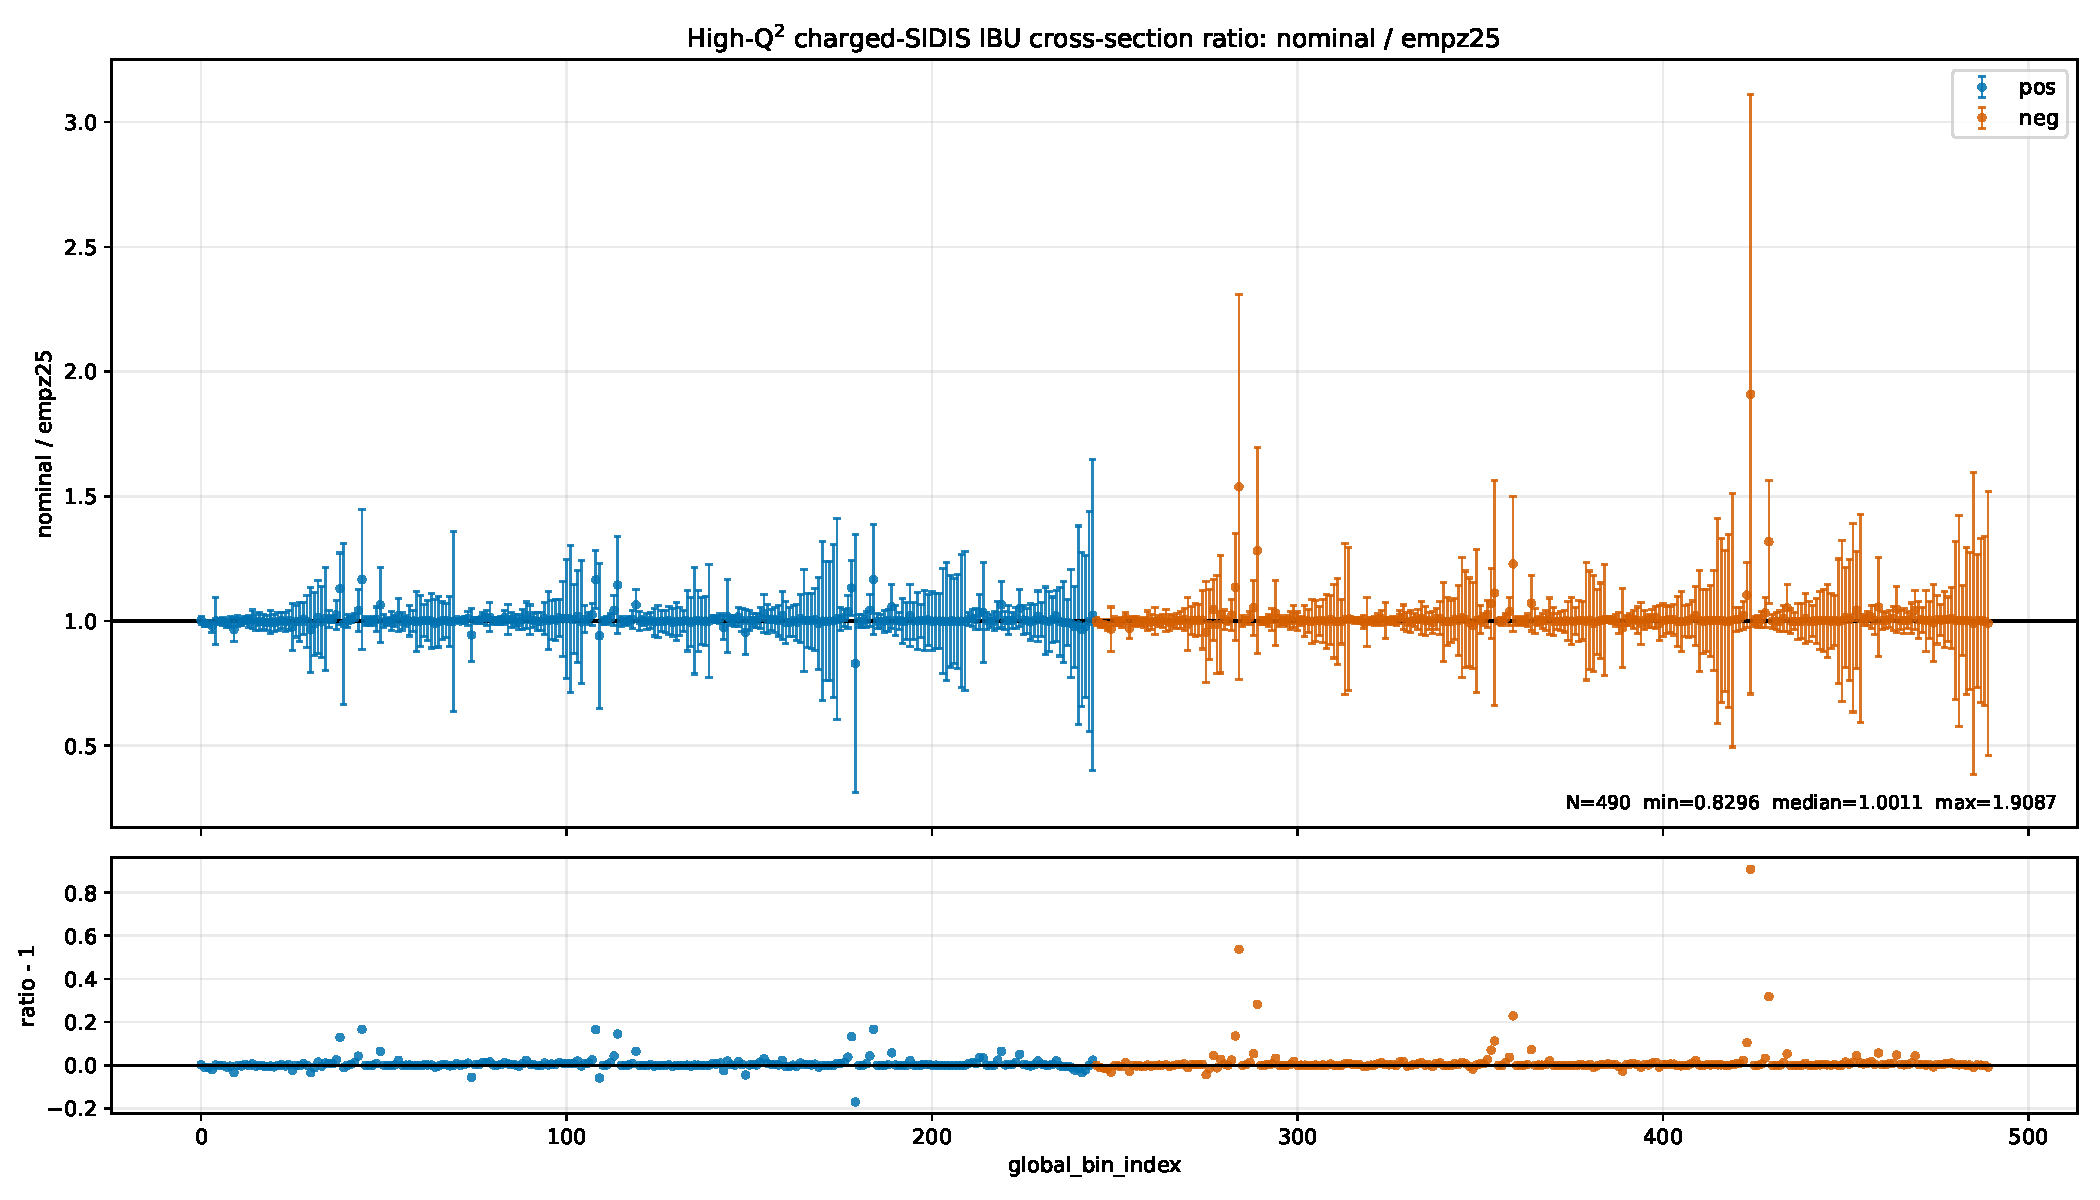
\includegraphics[width=0.95\textwidth]{figures/fig_cutvar_empz25_ratio.pdf}
  \caption{Global bin ratio of the unfolded cross sections for the reconstructed
  \mbox{$E-p_z>35\,\mathrm{GeV}\to E-p_z>25\,\mathrm{GeV}$} threshold variation.}
  \label{fig:syst:cutvar-empz25}
\end{figure}

\begin{figure}[p]
  \centering
  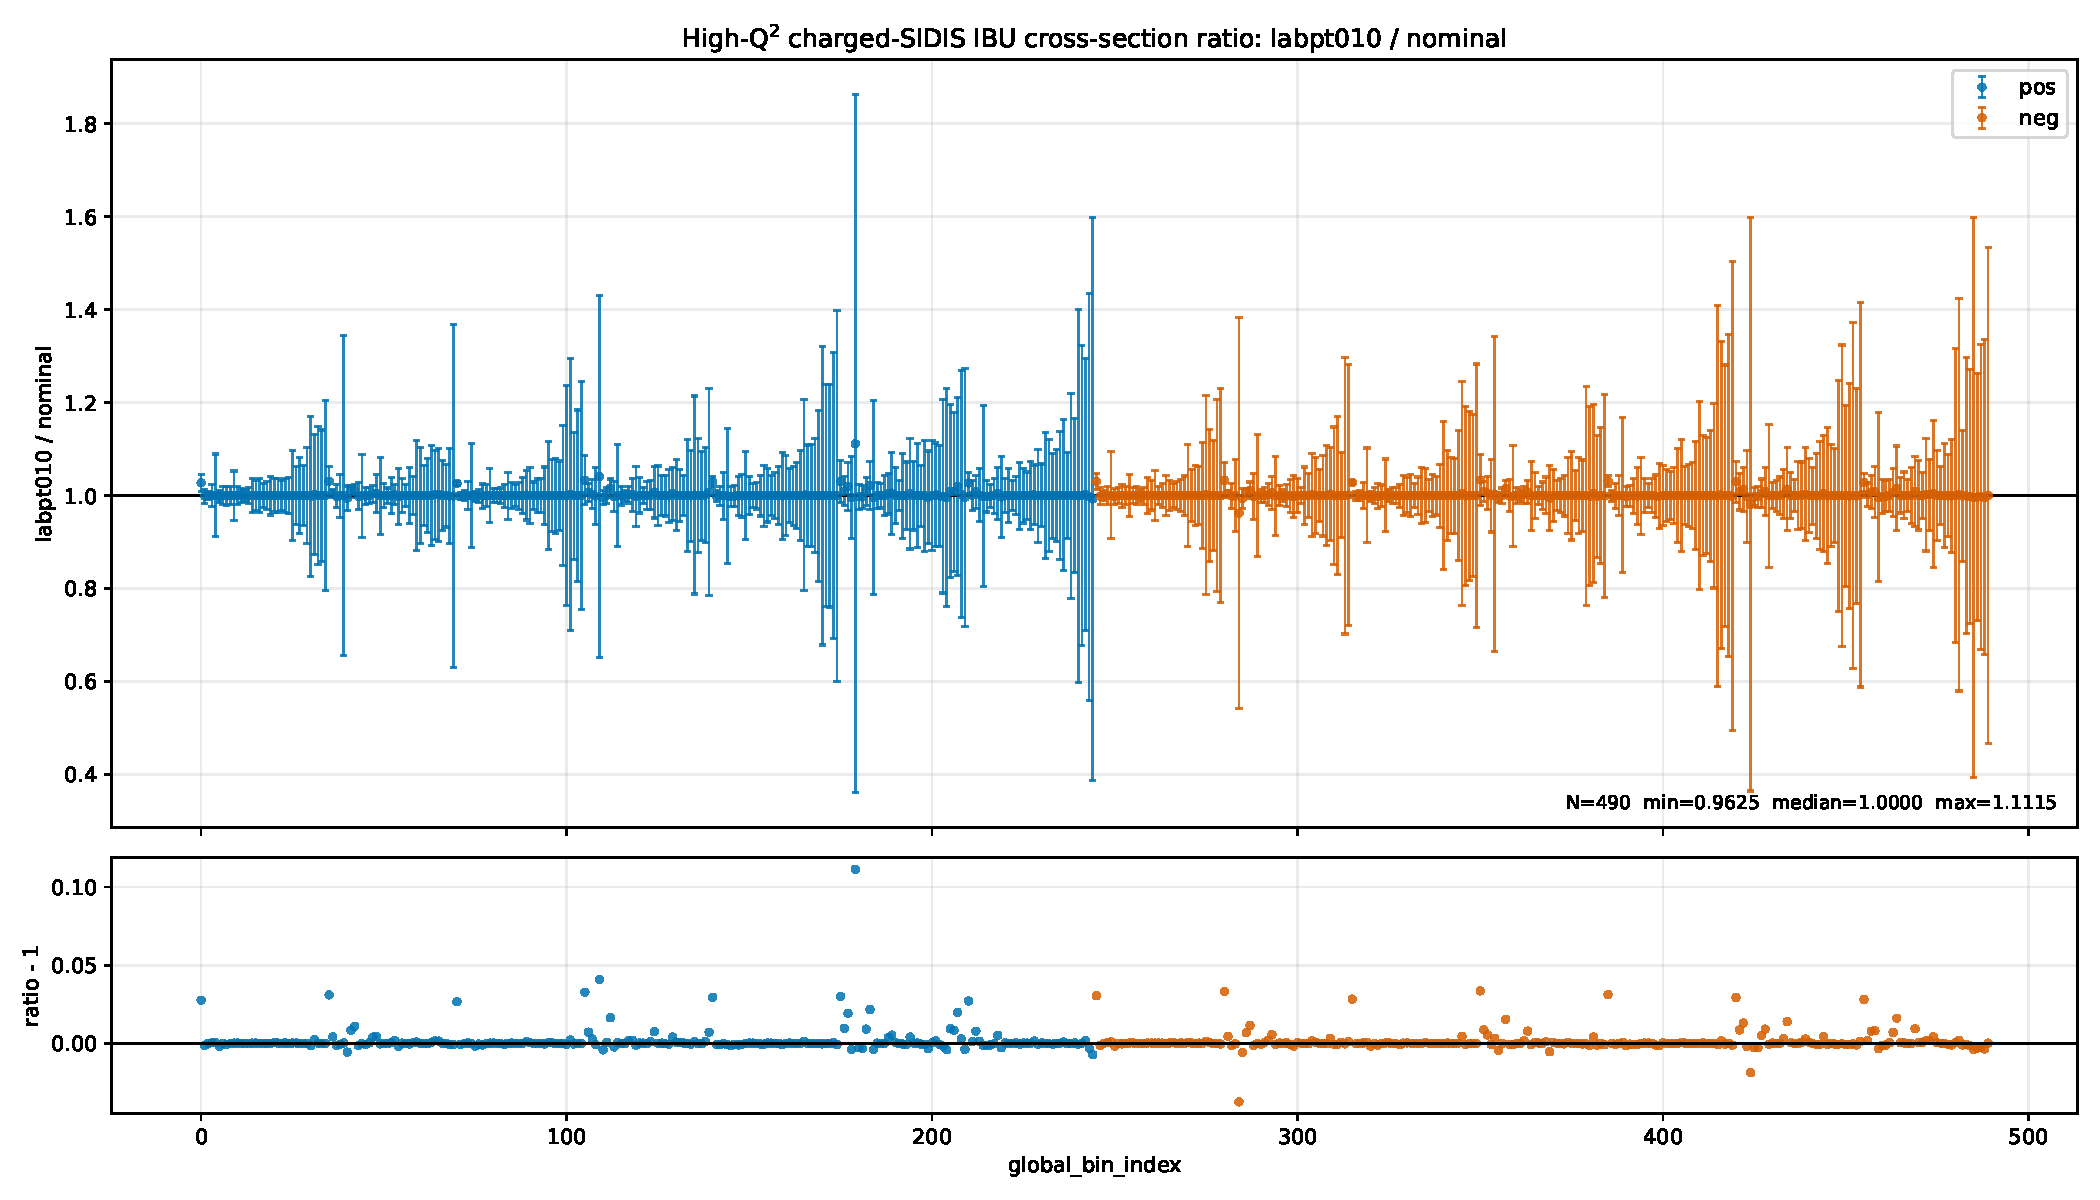
\includegraphics[width=0.95\textwidth]{figures/fig_cutvar_labpt010_ratio.pdf}
  \caption{Global bin ratio of the unfolded cross sections for the reconstructed lab-frame \mbox{\(p_T<0.15\,\mathrm{GeV}\to p_T<0.10\,\mathrm{GeV}\)}threshold
  variation.}
  \label{fig:syst:cutvar-labpt}
\end{figure}

\begin{figure}[p]
  \centering
  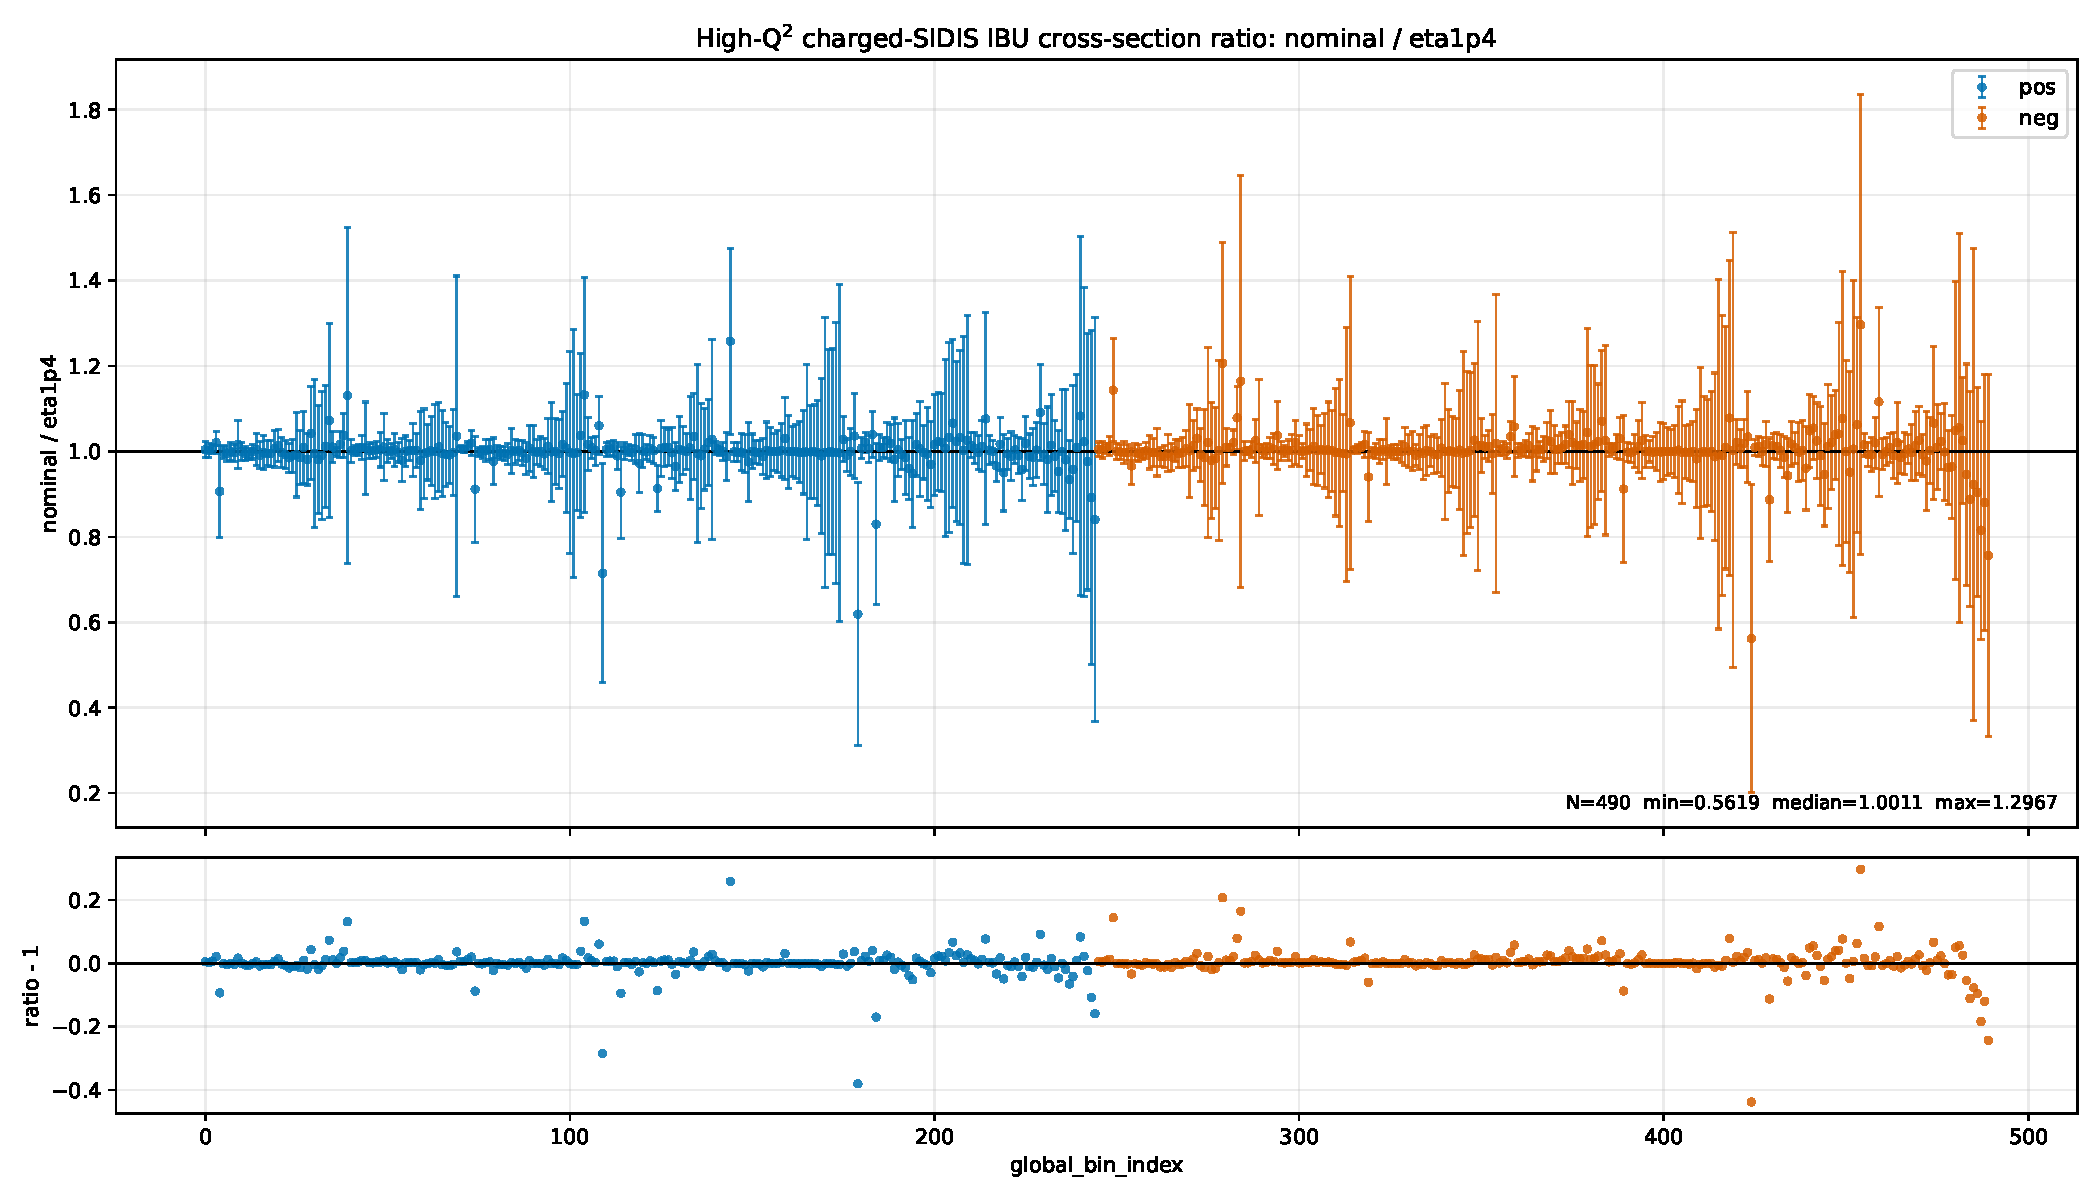
\includegraphics[width=0.95\textwidth]{figures/fig_cutvar_eta1p4_ratio.pdf}
  \caption{Global bin ratio of the unfolded cross sections for the reconstructed lab-frame \mbox{$|\eta|<1.6\to|\eta|<1.4$} threshold
  variation.}
  \label{fig:syst:cutvar-eta}
\end{figure}

\begin{figure}[p]
  \centering
  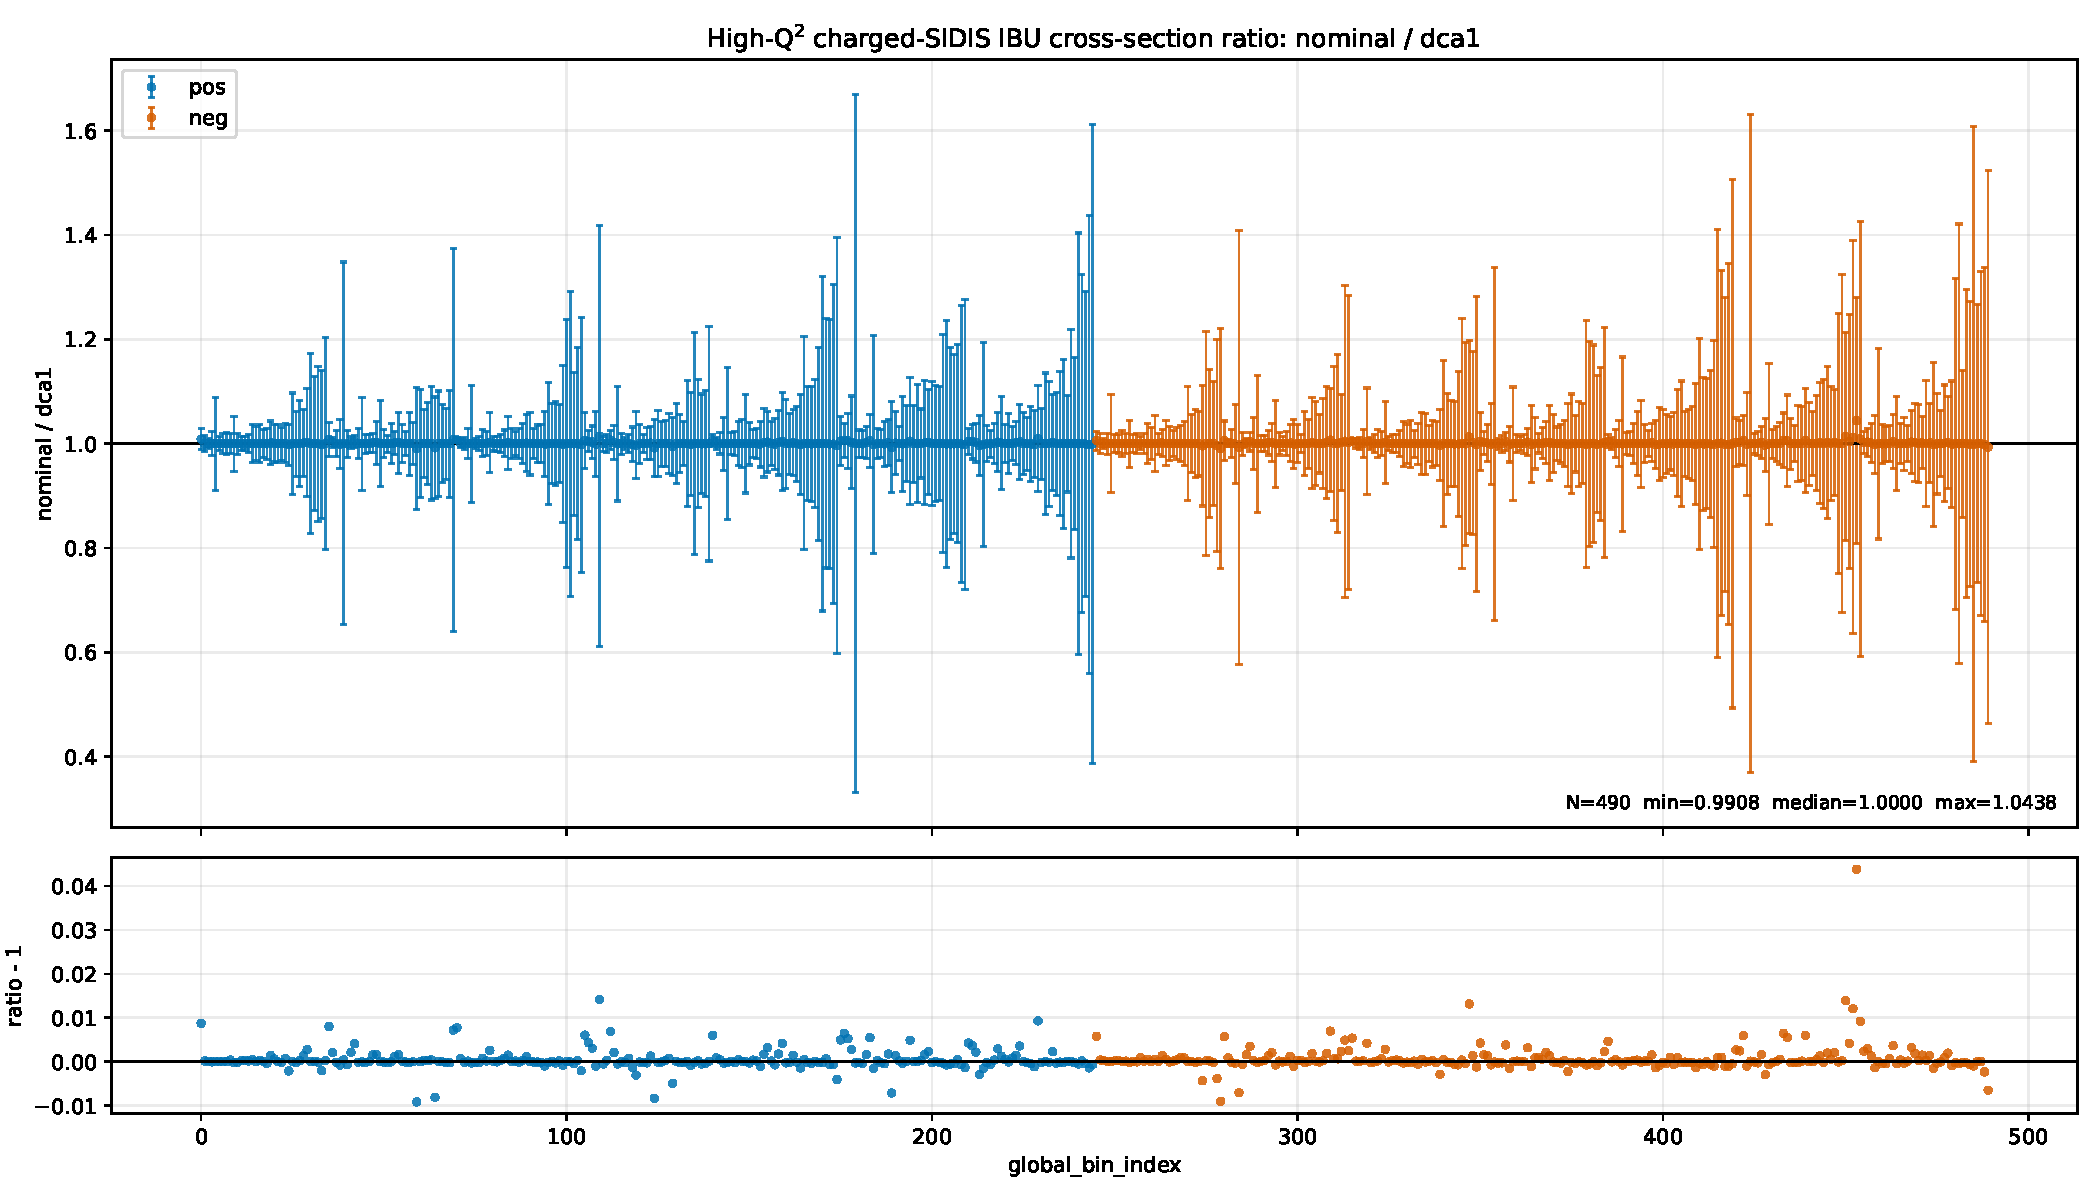
\includegraphics[width=0.95\textwidth]{figures/fig_cutvar_dca1_ratio.pdf}
  \caption{Global bin ratio of the unfolded cross sections for the reconstructed
  \mbox{$\mathrm{DCA}'\sin\theta < 2\,\mathrm{cm} \to \mathrm{DCA}'\sin\theta < 1\,\mathrm{cm}$}
  threshold variation.}
  \label{fig:syst:cutvar-dca1}
\end{figure}

\begin{figure}[p]
  \centering
  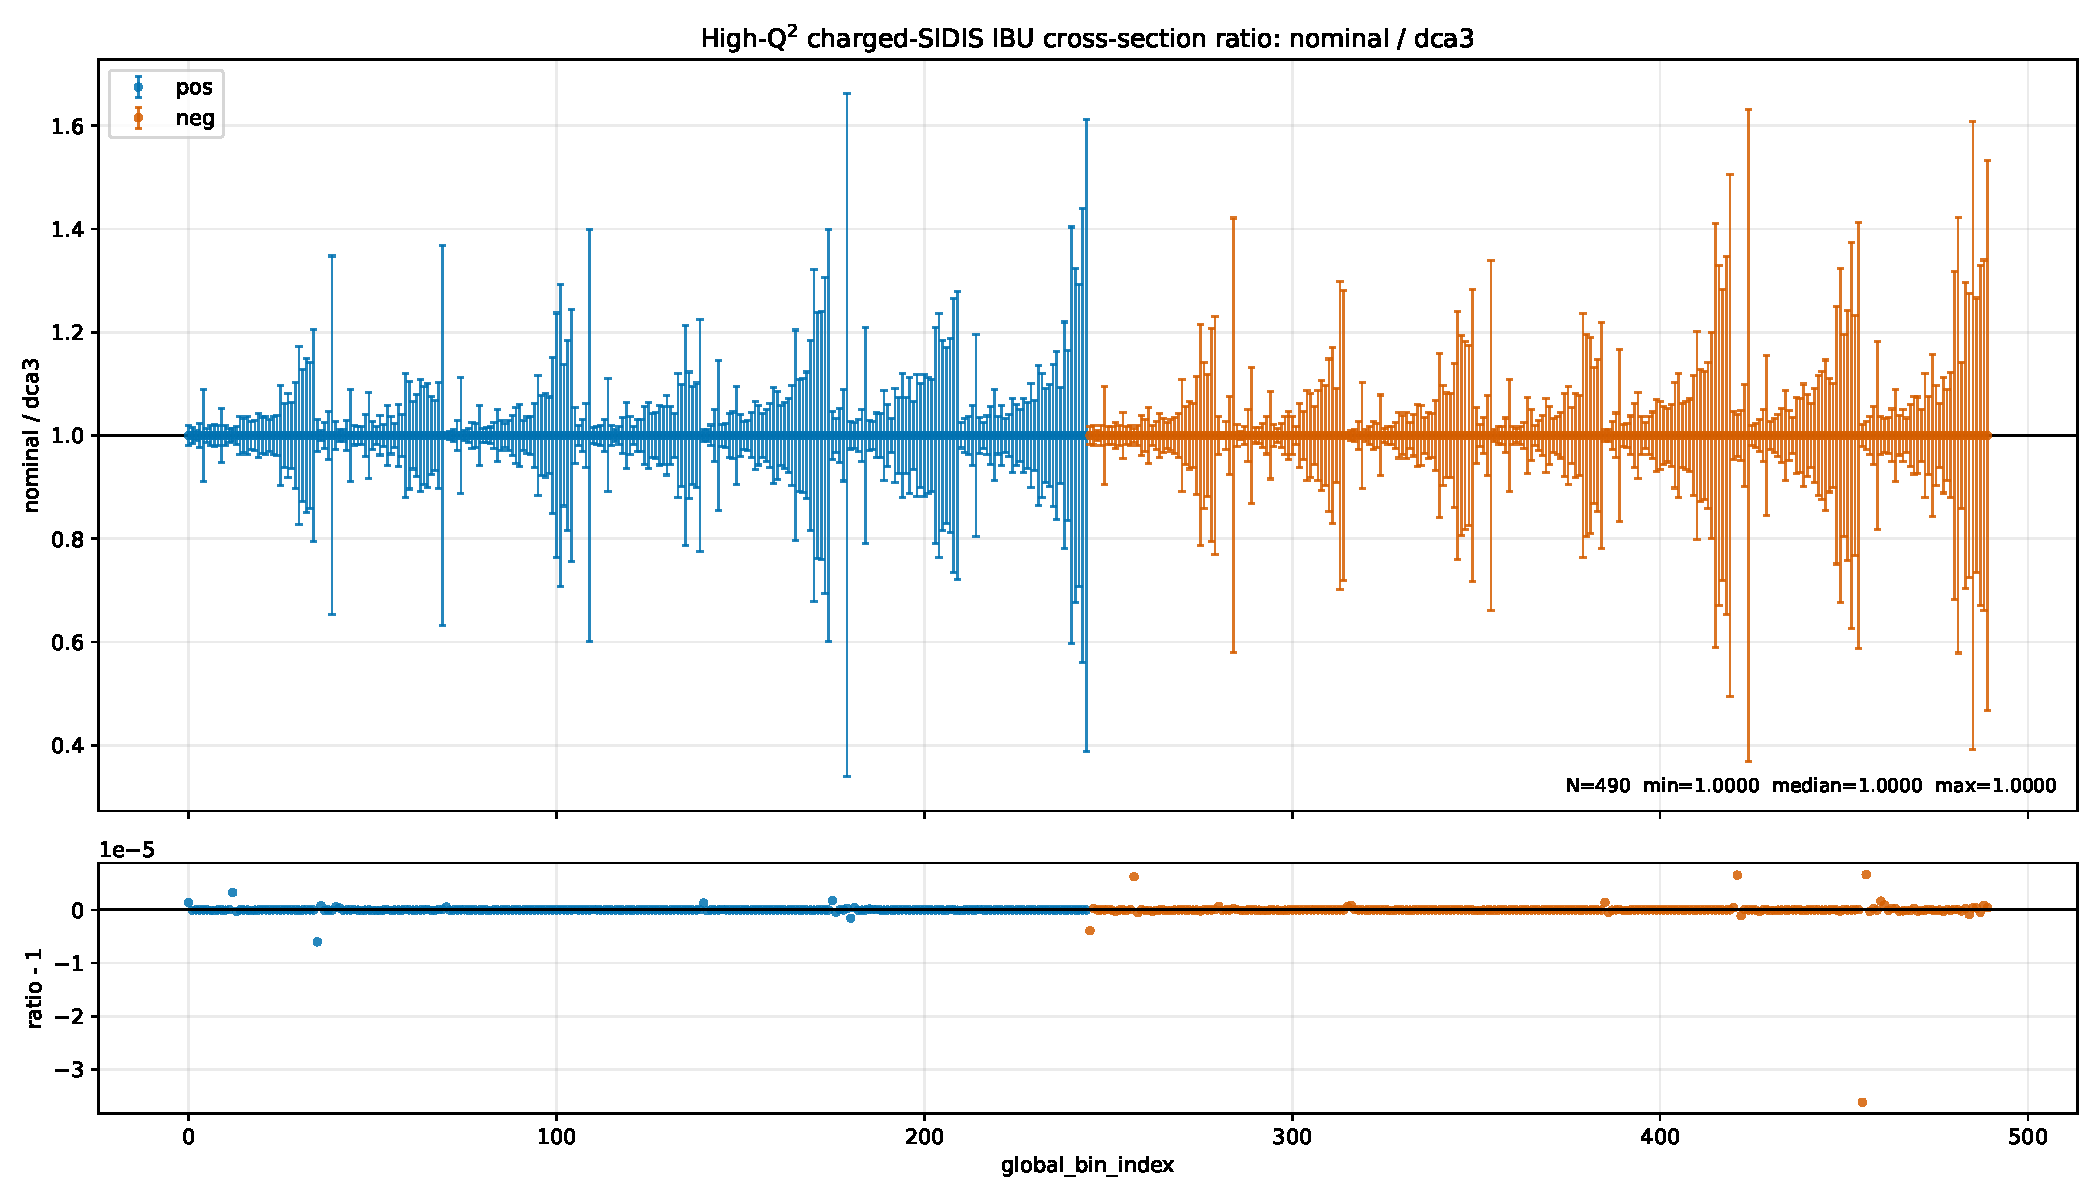
\includegraphics[width=0.95\textwidth]{figures/fig_cutvar_dca3_ratio.pdf}
  \caption{Global bin ratio of the unfolded cross sections for the reconstructed
  \mbox{$\mathrm{DCA}'\sin\theta < 2\,\mathrm{cm} \to \mathrm{DCA}'\sin\theta < 3\,\mathrm{cm}$}
  threshold variation.}
  \label{fig:syst:cutvar-dca3}
\end{figure}

\subsection{Near-Electron Opening-Angle Diagnostic}
\label{sec:syst:near-electron-alpha}
The previous H1 results (Refs.~\cite{H1:2013qsm,H1:2020zpd}) use a track--scattered-electron angle requirement larger than 0.2 rad to suppress anomalous tracks appearing near the scattered electron. These tracks could arise from photon conversions of final-state radiation (at the vertex or in detector material) off the electron, or tracks from the scattered electron which are mis-identified as not belonging to the scattered electron~\cite{Grebenyuk:2012thesis}. In the latter case, it would be expected that the track energy would be relatively close to the scattered electron energy measured in the calorimeter. The reconstructed momentum of the tracks very near to the scattered electron does not correlate strongly to the scattered electron energy, supporting the photon conversion hypothesis over the electron track mis-ID hypothesis.

Since the cone-baseline promotion of 2026-10-13, the
$\alpha\ge0.2~\mathrm{rad}$ laboratory-frame cone on the reconstructed legs is
part of the central selection basis rather than a diagnostic variant.  The
cone is applied after the electron and V0 truth vetoes and before the
matched-fake classification; cone-rejected matched legs flow to the miss row
of the response, and the coherent prior is computed from the response variant
that carries both the cone selection and the detector-interaction correction.
The diagnostic ratios in
Table~\ref{tab:syst:alpha-veto-integrated} were produced before that
promotion and are retained as motivation for the cone requirement.

\begin{table}[h]
\centering
\small
\begin{tabular}{p{4.4cm}p{2cm}p{2cm}}
\toprule
Quantity for $\alpha<0.2$ & RAPGAP & DJANGOH \\
\midrule
Integrated true $\pi/K/p$ loss & 0.106\% & 0.114\% \\
Residual $e^{\pm}$ / true $\pi/K/p$
  & $4.38\%$
  & $4.39\%$ \\
%V0-daughter / true $\pi/K/p$
%  & $3.90\%$
%  & $3.88\%$ \\
\bottomrule
\end{tabular}
\caption{Integrated MC-only diagnostic ratios for the near-electron opening-angle
study.}
\label{tab:syst:alpha-veto-integrated}
\end{table}

% Results section for the H1 high-Q^2 charged-particle SIDIS analysis note.
\section{Results}
\label{sec:results}

\begin{tcolorbox}[colback=yellow!8,colframe=orange!70,title={\bfseries Current release status}]
The current nominal central-value chain is the 2026-10-20 OPT-A baseline
promotion, in which the response truth contract is harmonized to the
radiative correction (Sec.~\ref{sec:unfolding:truth-contract}).  Its
reconstructed-level definition combines the $\alpha\ge0.2~\mathrm{rad}$
laboratory-frame scattered-electron cone with the
detector-interaction-corrected response, and the electron, V0, and
low-$\Qsq$ background templates are subtracted from the data vector before
unfolding.  The cross section is Born-level provisional:
$C_{\mathrm{rad}}$ is applied per-bin post-unfold from the DJANGOH14 table
binned as the release, with its uncertainty carried as the radiative
generator-difference and radiative-statistics components.  The
$E-p_z>45~\GeV$ convention is retained.  The systematic budget is being
regenerated on this nominal: the frozen budget editions on file were
computed on the superseded central values, are superseded as a quoting
basis, and no per-bin uncertainty or uncertainty total is final until the
regenerated budget passes review
(Sec.~\ref{sec:syst:budget-regeneration}).  The 2026-10-17 clean release
and the 2026-10-15 Born release are superseded for the nominal and retained
untouched as provenance.  The exposure of the simulated
radiative samples is reconciled file by file, but the generator-log
cross-check is permanently blocked externally, so the radiative correction
remains provisional and the release is not publication-grade.  The
$C_{\mathrm{rad}}$ multiplicity mapping and the
corrected inclusive DIS denominator are still pending.  Numerical
multiplicities and final physics tables should therefore be regarded as
preliminary until the denominator is available.
\end{tcolorbox}

\subsection{Working Release}
\label{sec:results:z005-release}

The current high-$\Qsq$ working release contains 490 published bins in total,
with 245 $\hplus$ rows and 245 $\hminus$ rows.  The nominal unfolding method is
iterative Bayesian unfolding with four selected iterations.  The data vector
length is 980, and the per-charge response shape is $(491,246)$.

The canonical raw release is
\path{bbb_ibu_bgsub_setRprime_conebase_optA_q2esgen_S3xmerged_zlow005_pT5_eta1p6_radlen5_nhit5_2026-10-20/}
under \path{H1ChargedSidis_HighQ2/output_v6/central/data_release/}, and its
Born-level product is the in-tree \path{born_crad_applied/} directory of the
same release.  Both use the response matrix's own generator-level
distribution as the unfolding prior, on the harmonized response of
Sec.~\ref{sec:unfolding:truth-contract}.  Integrated over the 490 published
bins at $\mathcal{L}_{\mathrm{data}}=351000.0~\mathrm{nb}^{-1}$, the raw
release gives IBU $10.511329~\mathrm{nb}$ ($\hplus$) and
$10.219863~\mathrm{nb}$ ($\hminus$); the Born-level product gives IBU
$11.997446~\mathrm{nb}$ ($\hplus$) and $11.664706~\mathrm{nb}$
($\hminus$).

This release supersedes for the nominal the 2026-10-17 clean release
\path{bbb_ibu_bgsub_setRprime_conebase_S3xmerged_zlow005_pT5_eta1p6_radlen5_nhit5_2026-10-17/}
and its 2026-10-15 Born parent
\path{born_crad_bgsub_setRprime_conebase_S3xmerged_zlow005_pT5_eta1p6_radlen5_nhit5_2026-10-15/},
which are retained untouched as provenance; their integrated values
($10.508811~\mathrm{nb}$ and $10.217503~\mathrm{nb}$ raw,
$11.996558~\mathrm{nb}$ and $11.663956~\mathrm{nb}$ Born) are superseded
central values.  The promotion moves the integrated raw totals by $+0.0240\%$
($\hplus$) and $+0.0231\%$ ($\hminus$) and the Born totals by $+0.0074\%$ and
$+0.0064\%$.  Per cell, the Born shifts have absolute medians of $1.05\%$
($\hplus$) and $1.15\%$ ($\hminus$), and the largest populated shift is
$+4.2051\%$ (negative charge, global bin 159), below its full-sample net
straddle rate of $+4.9191\%$ (ratio $0.855$); every well-populated per-cell
shift is bounded by its full-sample per-cell straddle rate, the complete
exception set being the adjudicated 48-cell list of
Sec.~\ref{sec:unfolding:truth-contract}.  The change is a
one-time central-value correction---the removal of the response binning bias
documented in Sec.~\ref{sec:unfolding:truth-contract}---and is not carried
as an uncertainty.  The background
subtraction removes $281{,}250.09$ tracks, $7.2767\%$, from the cone data
vector of $3{,}865{,}073$ in-grid entries before the unfolding:
$148{,}976.4$ electron and positron tracks, $132{,}065.3$ V0 decay daughters,
and $208.4$ low-$\Qsq$ leakage tracks.  The subtracted data vector itself is
unchanged by the promotion.  The detector-interaction class is not
part of this external subtraction: it is removed response-internally through
the per-reco-bin fake fraction $f_i$ of the detector-interaction-corrected
response, and an external subtraction of it would double-remove the class.
For lineage, the immediately preceding release with the electron cone but no
background subtraction, which unfolds the full cone data vector, integrates to
raw IBU
values of $11.412233~\mathrm{nb}$ ($\hplus$) and $11.123626~\mathrm{nb}$
($\hminus$); these superseded values are retained only as the historical
parent of the current release and are not current results.

The systematic budget is being regenerated on this nominal
(Sec.~\ref{sec:syst:budget-regeneration}).  The most recent frozen editions,
the twenty-active-term 2026-10-19 edition and its nineteen-component
2026-10-17 parent, were computed on the superseded central values; they are
superseded as a quoting basis and retained unchanged as provenance, and the
per-bin uncertainties and totals of those editions must not be quoted as
final until the regenerated budget passes review.  The component inventory
of those editions is described in
Sec.~\ref{sec:systematics}.

The central IBU implementation has an independent numerical cross-check:
RooUnfoldBayes reproduces the in-house iterative-Bayesian yields to a maximum
relative precision of $2.6\times10^{-15}$ across 980 rows.  This comparison
covers both RAPGAP and DJANGOH response inputs and has no invalid or
zero-denominator bins.

\subsection{Diagnostic Four-Dimensional Cross-Section Plots}
\label{sec:results:diagnostic-4d-cross-sections}

The plotted observable used for diagnostic data--MC comparisons is the
four-dimensional differential cross section,
\begin{equation}
  \frac{\mathrm{d}^{4}\sigma}{\mathrm{d}\Qsq\,\mathrm{d}x\,
  \mathrm{d}z\,\mathrm{d}\pTh}
  = \frac{\sigma_{\mathrm{bin}}}{\Delta\Qsq\,\Delta x\,\Delta z\,\Delta\pTh},
  \label{eq:results:four-dimensional-cross-section-density}
\end{equation}
in units of $\mathrm{nb}\,\GeV^{-3}$, since the $\mathrm{d}\Qsq$ differential
contributes $\GeV^{2}$. For the capped top-$x$ cell, $\Delta x=1.0-x_{\min}$.

The current five-prediction comparison package is
\path{plots/mc_predictions/data_vs_mc_z005_5generator_born_releasebin_2026-10-13/}.
Its data side is the superseded raw release without the electron cone,
corrected to the photon-Born level without the $Z$-exchange contribution.  It is a DJANGOH-only provisional diagnostic: the
four generator curves are at full-Born/NORAD level while the data side is
photon-Born, producing a known level difference of about $9\%$ by design;
only MAPTMD24 is photon-only.  The package has not been regenerated on the
current cone-based observable basis and its figures are not referenced in this
note.  MAPTMD24 covers 230 of 490 published bins, with no $z<0.05$ row and
sparse $\pTh$ coverage at higher $z$; this is the final limitation of that
comparison.  The package remains a PROVISIONAL INTERNAL DIAGNOSTIC.

\subsection{Diagnostic Cross-Section Density with the Near-Electron Veto}
\label{sec:results:diagnostic-alpha0p2-cross-section-density}

Figures~\ref{fig:results:alpha0p2-xsec-density-hplus} and
\ref{fig:results:alpha0p2-xsec-density-hminus} show the IBU-only
cross-section-density diagnostic for the near-electron opening-angle veto,
which rejects tracks with $\alpha<0.2$.  The plotted observable is the
four-dimensional differential cross section defined in
Eq.~\ref{eq:results:four-dimensional-cross-section-density}, using the same 4D
bin-volume normalization.  The input is the rescaled IBU release CSV from this
study, with $\mathcal{L}_{\mathrm{data}}=351~\pbinv$, the selection
$|\eta|<1.6$, radial track length at least $5~\mathrm{cm}$, and at least five
CJC hits, and the measurement binning.

The seven displayed $(\Qsq,x)$ intervals are listed in
Table~\ref{tab:binning:z005-contract}. Each charge plot contains these seven
cells, seven $z$ bins, and five $\pTh$ bins, for 490 plotted points in total
across both charges and no skipped bins. All densities use the physical cap
$\Delta x=1.0-x_{\min}$; the figures in this section were regenerated on
2026-10-16 with this convention.
The horizontal uncertainty is the $\pTh$ half-bin width.  The vertical
uncertainty is the quadrature sum of the statistical, model, and
regularization uncertainties, divided by the 4D bin volume; no additional
systematic components are included in these error bars.

The plots are retained here as diagnostic/provisional products only: they are
raw pre-Born inputs from an earlier, superseded release lineage, without
background subtraction or $C_{\mathrm{rad}}$.
Final approval remains pending; the plots are not for public release or
citation, and multiplicities remain blocked because no corrected inclusive DIS
denominator is available. For the cross section the radiative correction is no
longer pending: $C_{\mathrm{rad}}$ is applied per-bin post-unfold in the
current Born-level provisional release, with its uncertainty carried as the
radiative generator-difference and radiative-statistics components;
these selection-variant plots have not been regenerated on the current,
background-subtracted release.  Final release remains blocked by
publication-grade clearance of the radiative correction and by the
registration of the final publication plotting and systematics-rendering
chain.

\begin{figure}[p]
  \centering
  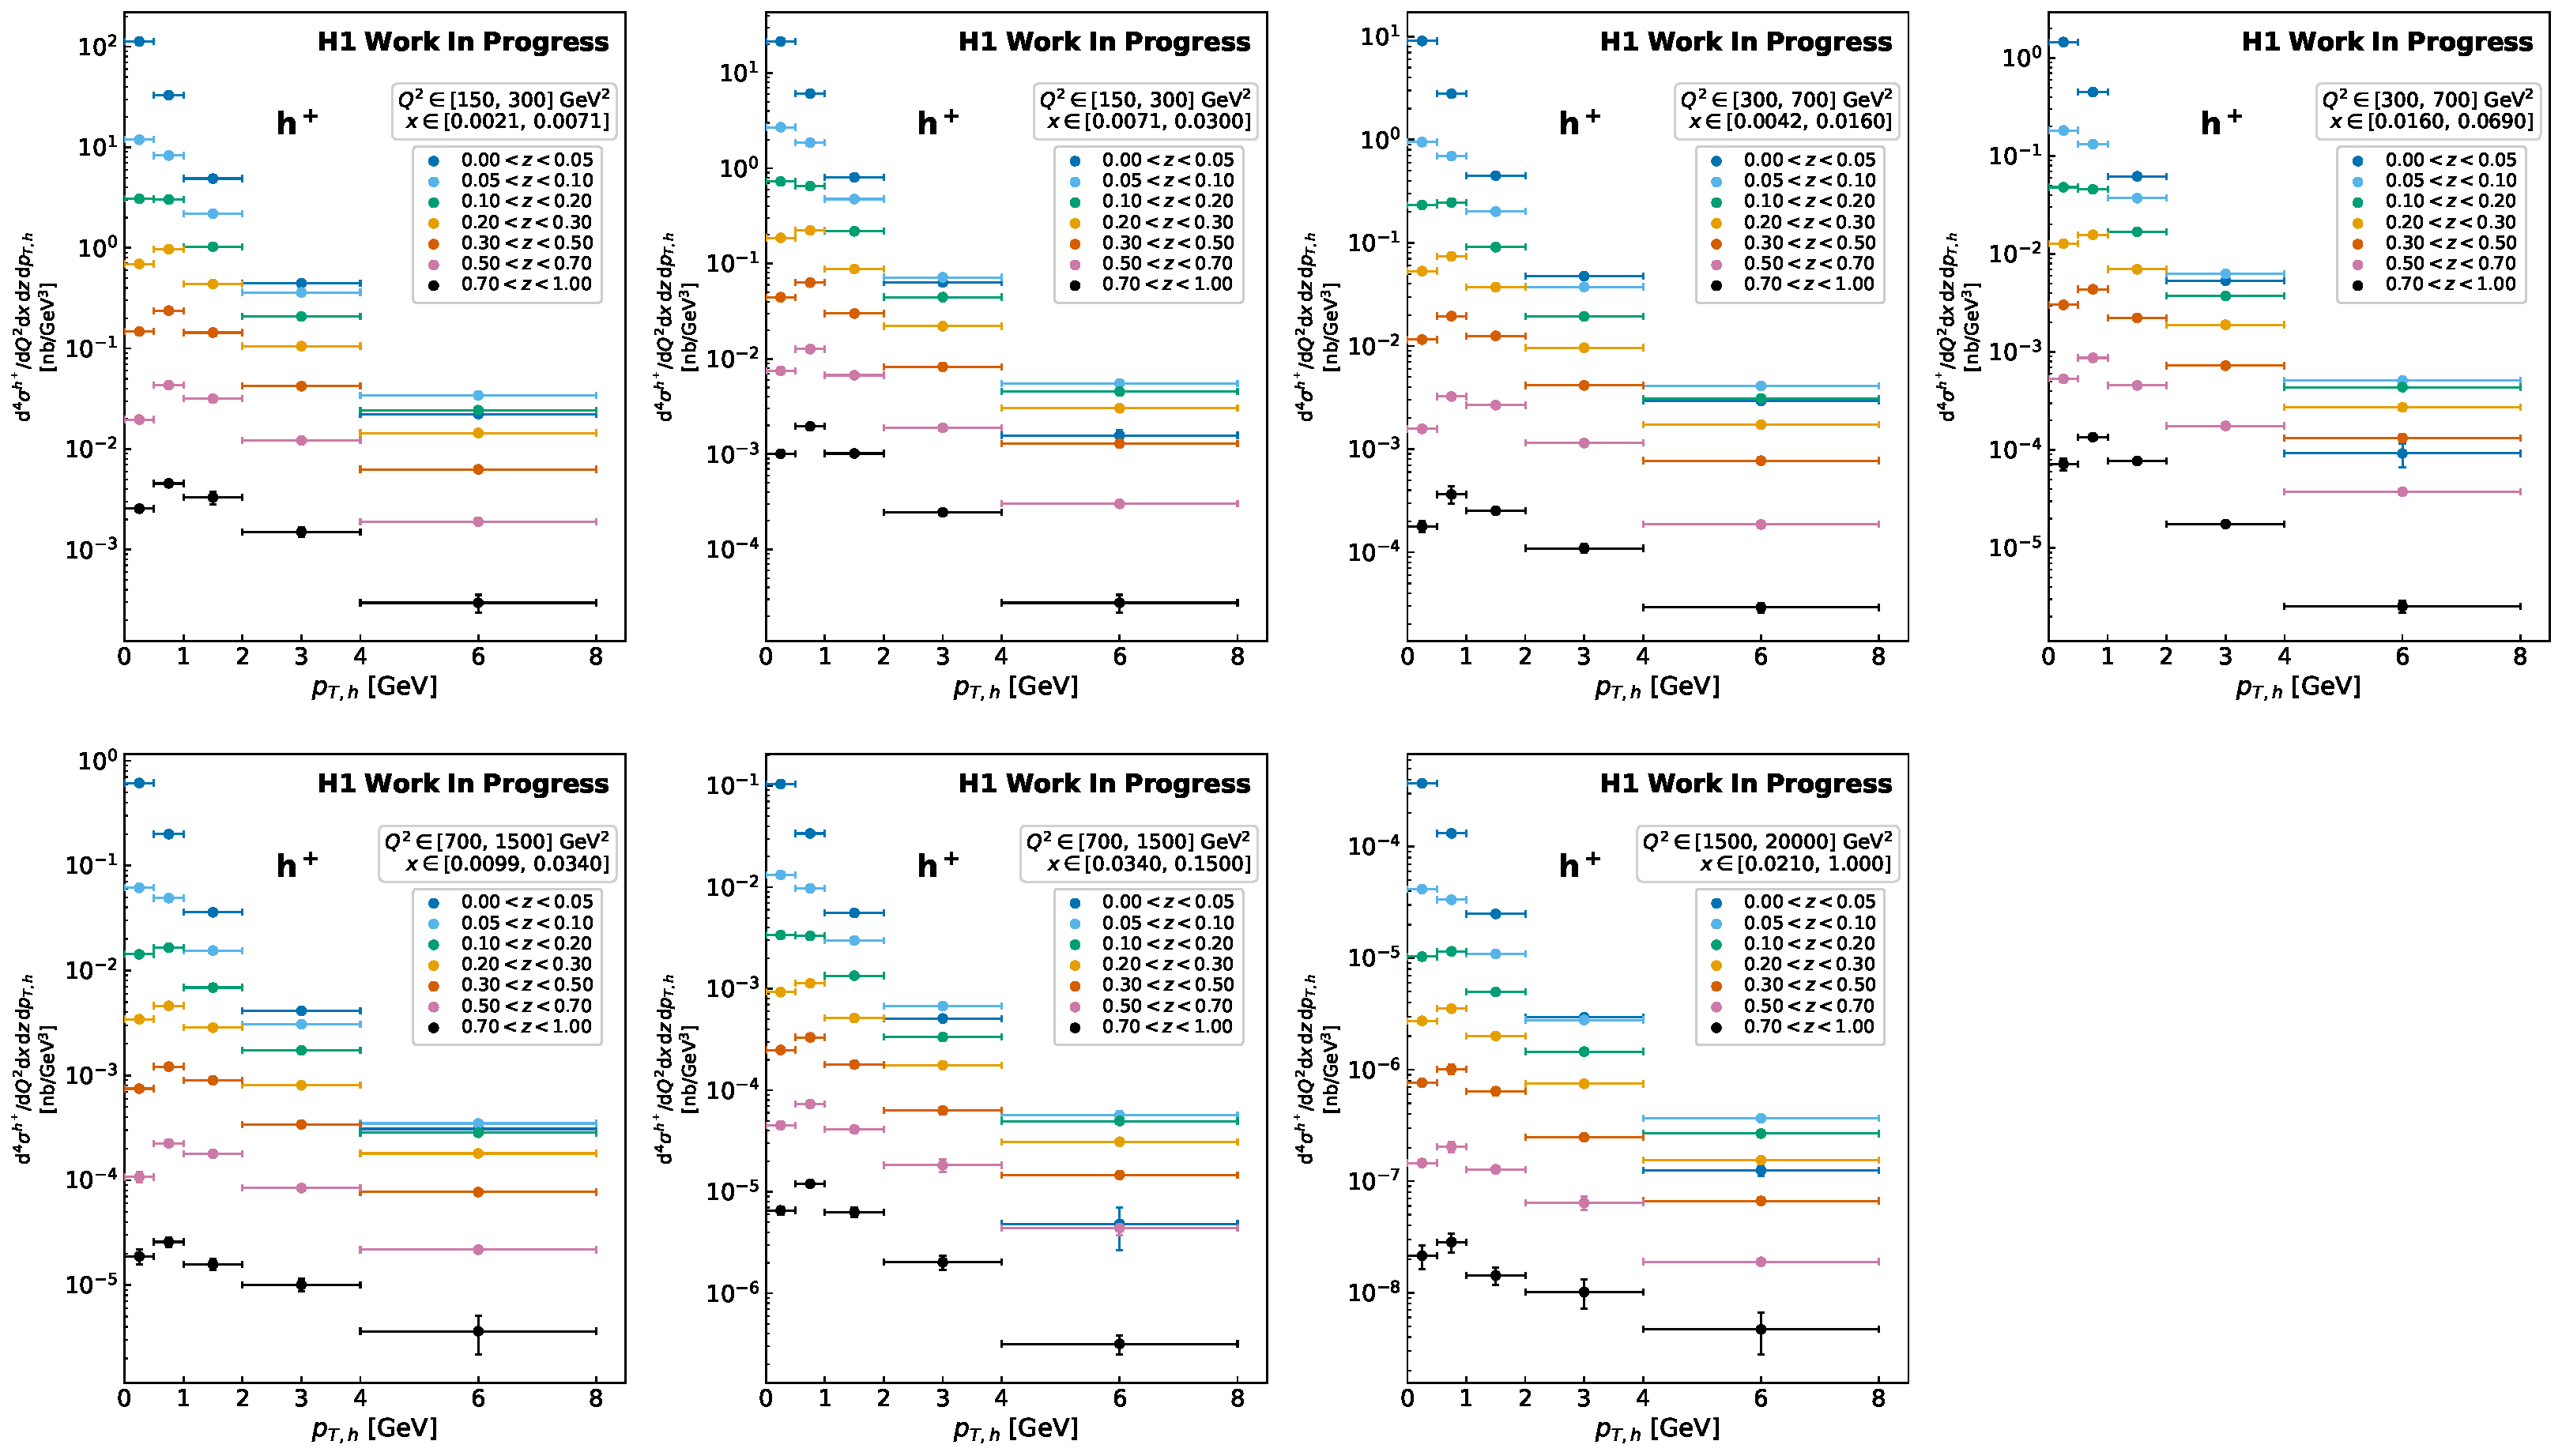
\includegraphics[width=0.98\textwidth,height=0.82\textheight,keepaspectratio]{figures/fig_results_xsec_density_alpha0p2_7panel_hplus_z005.pdf}
  \caption{Diagnostic/provisional cross-section density with the near-electron
  opening-angle veto for $\hplus$, plotted as
  $\mathrm{d}^{4}\sigma/(\mathrm{d}\Qsq\,\mathrm{d}x\,
  \mathrm{d}z\,\mathrm{d}\pTh)$ in $\mathrm{nb}\,\GeV^{-3}$.  The nominal
  iterative Bayesian unfolding is shown for $351~\pbinv$ in seven $(\Qsq,x)$ cells, seven $z$ bins,
  and five $\pTh$ bins.  Vertical uncertainties combine the statistical,
  model, and regularization contributions in quadrature and are divided by the
  4D bin volume; horizontal uncertainties are $\pTh$ half-bin widths.  No
  additional systematic components are included.  This raw pre-Born diagnostic
  is a superseded historical render with no background subtraction or
  $C_{\mathrm{rad}}$ correction, predating the current release, which applies
  both a pre-unfold background subtraction and the per-bin post-unfold
  $C_{\mathrm{rad}}$ correction; it is not for public release or citation.}
  \label{fig:results:alpha0p2-xsec-density-hplus}
\end{figure}

\begin{figure}[p]
  \centering
  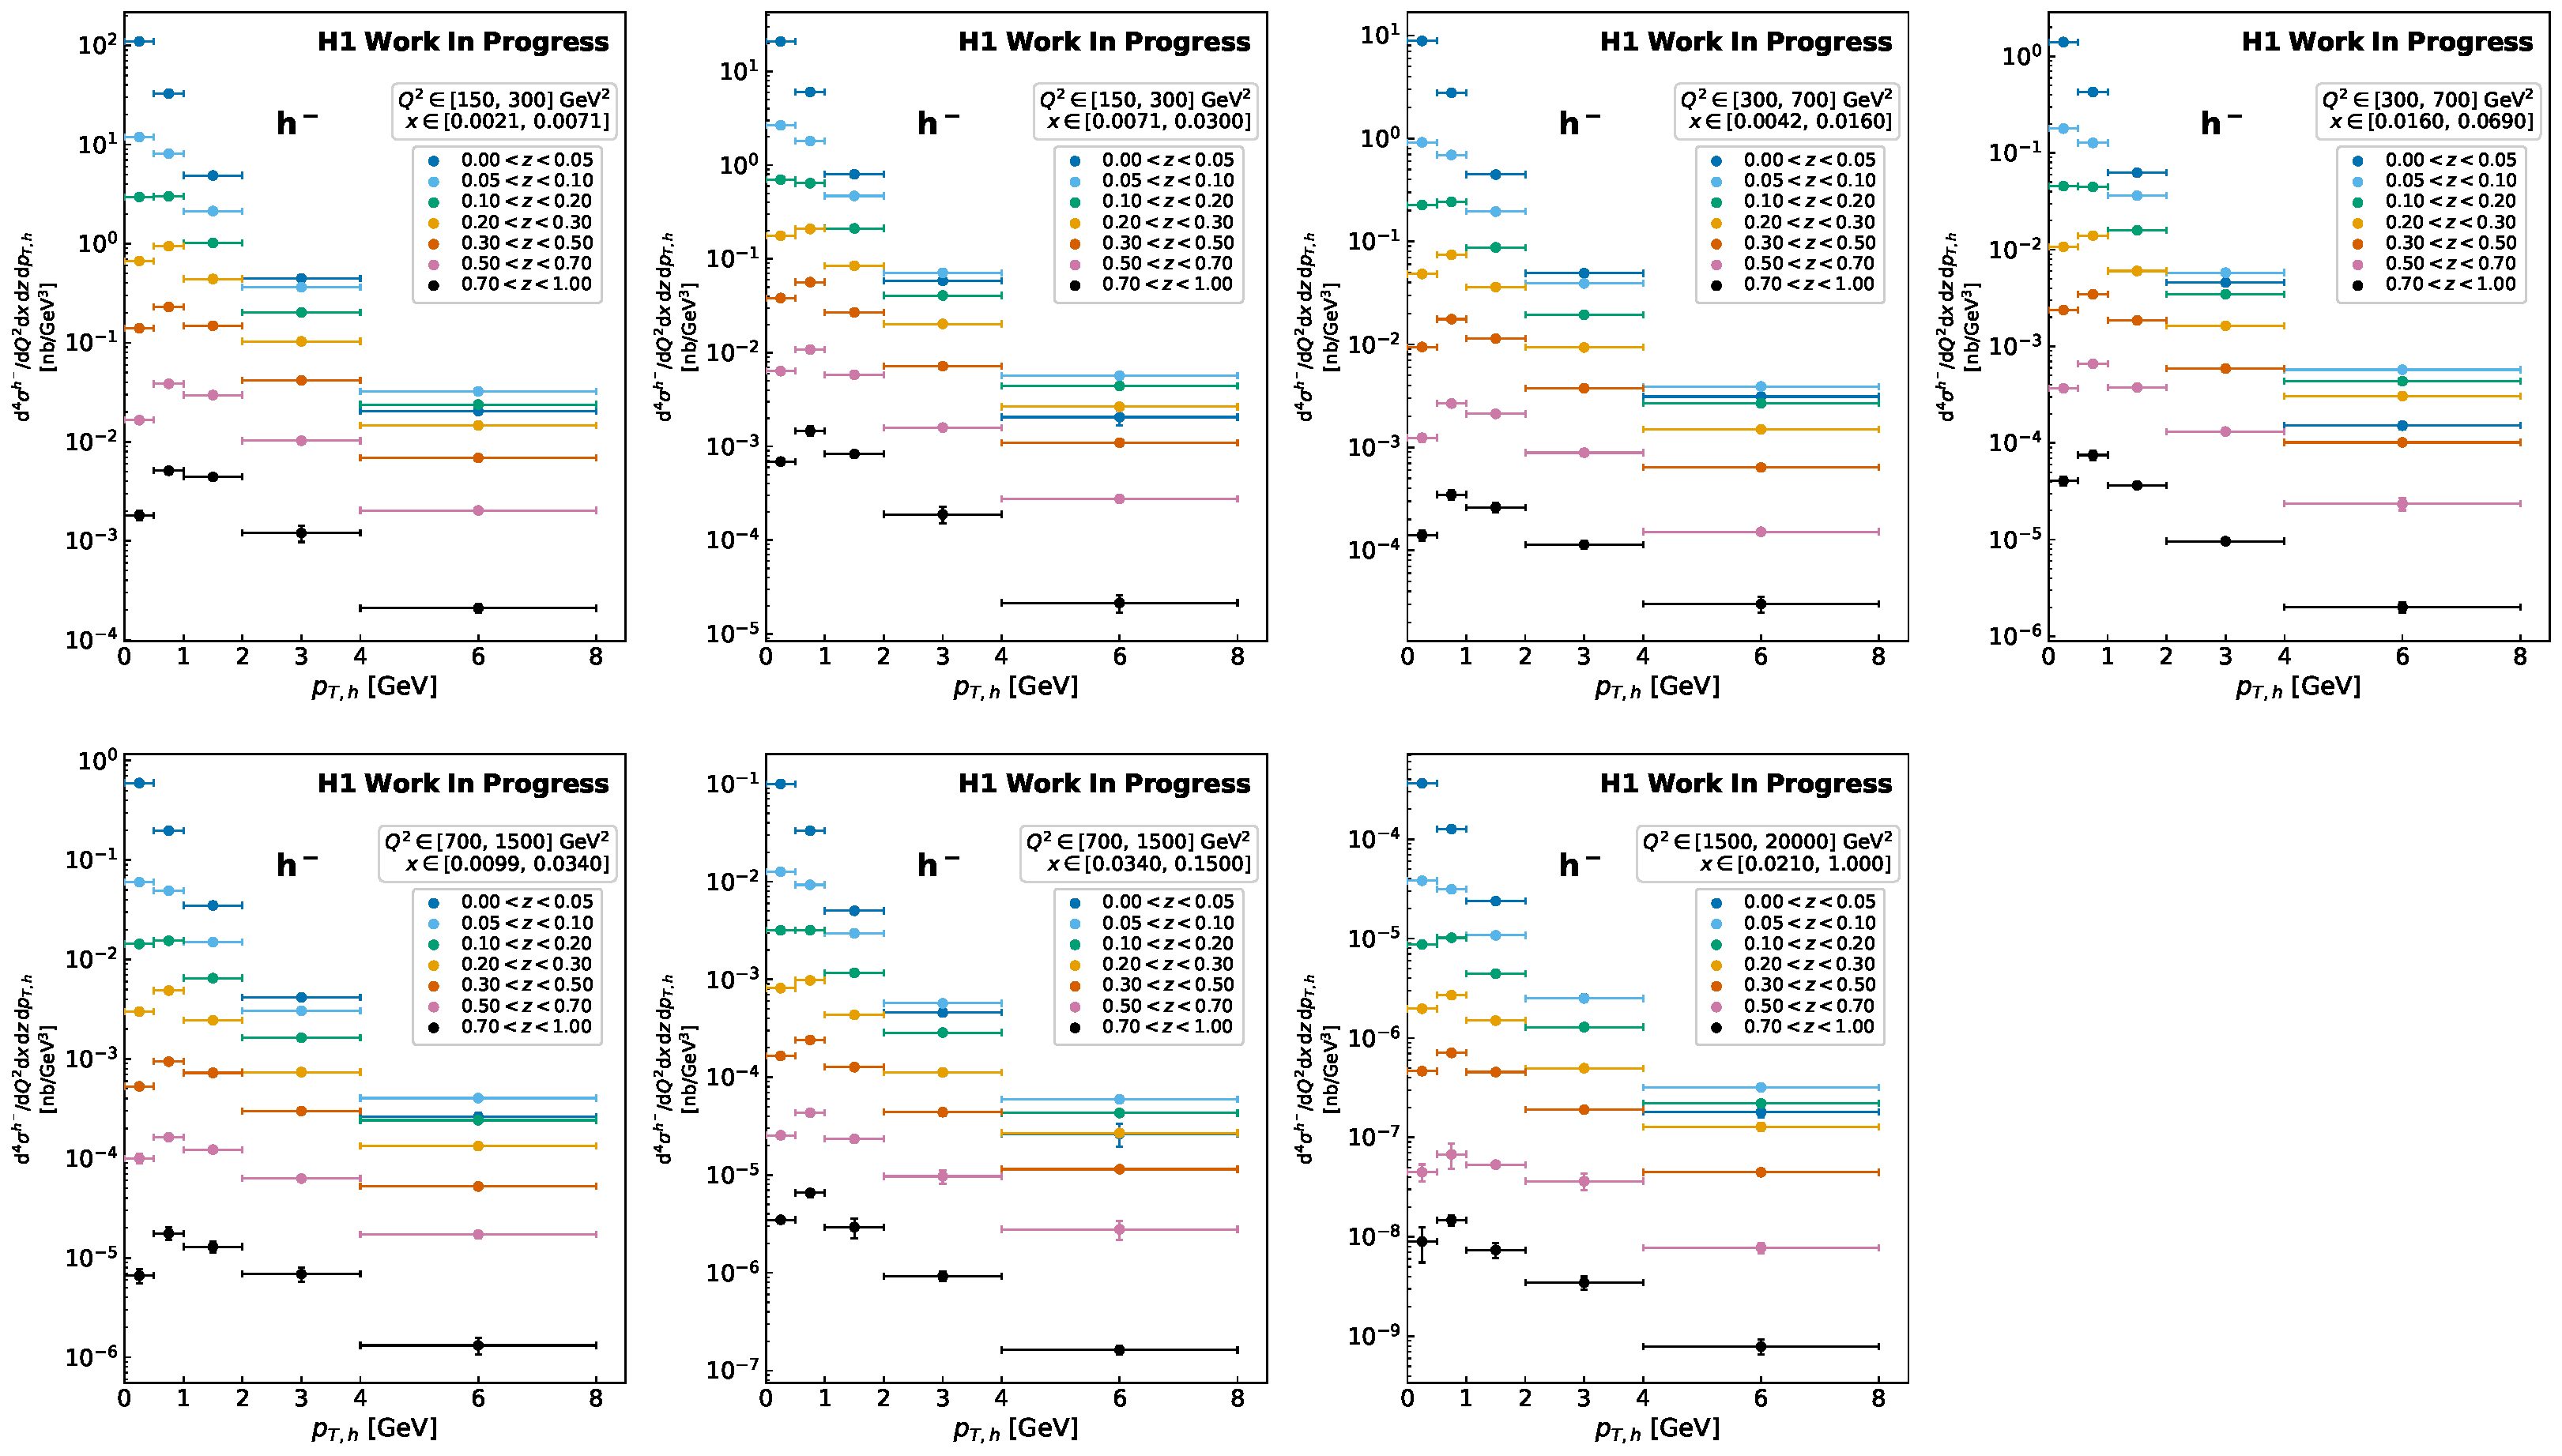
\includegraphics[width=0.98\textwidth,height=0.82\textheight,keepaspectratio]{figures/fig_results_xsec_density_alpha0p2_7panel_hminus_z005.pdf}
  \caption{Diagnostic/provisional cross-section density with the near-electron
  opening-angle veto for $\hminus$, plotted as
  $\mathrm{d}^{4}\sigma/(\mathrm{d}\Qsq\,\mathrm{d}x\,
  \mathrm{d}z\,\mathrm{d}\pTh)$ in $\mathrm{nb}\,\GeV^{-3}$.  The nominal
  iterative Bayesian unfolding is shown for $351~\pbinv$ in seven $(\Qsq,x)$ cells, seven $z$ bins,
  and five $\pTh$ bins.  Vertical uncertainties combine the statistical,
  model, and regularization contributions in quadrature and are divided by the
  4D bin volume; horizontal uncertainties are $\pTh$ half-bin widths.  No
  additional systematic components are included.  This raw pre-Born diagnostic
  is a superseded historical render with no background subtraction or
  $C_{\mathrm{rad}}$ correction, predating the current release, which applies
  both a pre-unfold background subtraction and the per-bin post-unfold
  $C_{\mathrm{rad}}$ correction; it is not for public release or citation.}
  \label{fig:results:alpha0p2-xsec-density-hminus}
\end{figure}

\subsection{Born-Level Provisional Cross-Section Density}
\label{sec:results:release351-expanded-xsec-density}

Figures~\ref{fig:results:release351-cone-xsec-density-hplus}
and~\ref{fig:results:release351-cone-xsec-density-hminus} show the Born-level
provisional cross-section densities of the background-subtracted
clean-release chain, obtained with the iterative Bayesian unfolding and the
response matrix's own generator-level prior.  The observable is
defined in Eq.~\ref{eq:results:four-dimensional-cross-section-density}.
These renders predate the 2026-10-20 OPT-A baseline promotion: their input is
the Born-level release
\path{born_crad_bgsub_setRprime_conebase_S3xmerged_zlow005_pT5_eta1p6_radlen5_nhit5_2026-10-15/}
under \path{H1ChargedSidis_HighQ2/output_v6/central/data_release/}, at
$\mathcal{L}_{\mathrm{data}}=351000.0~\mathrm{nb}^{-1}$, whose integrated IBU
totals, $11.996558~\mathrm{nb}$ for $\hplus$ and $11.663956~\mathrm{nb}$ for
$\hminus$ over the 490 published bins, are superseded central values
(Sec.~\ref{sec:results:z005-release}); the figures are retained until the
canonical plotting chain is re-pointed to the OPT-A nominal and the
regenerated budget is available.  $C_{\mathrm{rad}}$ is applied
per-bin post-unfold from the DJANGOH14 (xFGen$<$0, EMPZ$>$45) table, whose
integrated factors are 1.142 for $\hplus$ and 1.141 for $\hminus$; the
EMPZ$>$45 convention is retained.  The plotted points are the
background-subtracted Born-level values: the electron, V0, and low-$\Qsq$
backgrounds are subtracted from the data vector before unfolding, and the
detector-interaction class is removed response-internally through the
per-reco-bin fake fraction $f_i$.  Each charge plot contains seven
$(\Qsq,x)$ cells, seven $z$ bins, and five $\pTh$ bins, for 490 points across
both charges.

The vertical uncertainty bands show the quoted total systematic uncertainty of
the frozen 2026-10-19 budget, including the two radiative components.  This
budget combines twenty active quadrature terms on the background-subtracted
basis; its median totals are $7.320288331169215\%$ for $\hplus$ and
$7.637124635311324\%$ for $\hminus$, and no bin exceeds $100\%$.  The frozen
editions were computed on the superseded central values and are superseded as
a quoting basis, so these bands are not final: no per-bin uncertainty or
total is final until the budget regenerated on the OPT-A nominal passes
review (Sec.~\ref{sec:syst:budget-regeneration}).  These are not final
central values: the release is Born-level provisional, not physics-final,
and the figures carry internal-review status only.

Two plot packages document the OPT-A promotion itself; both were accepted on
visual review and neither carries final uncertainties.  The user-facing
new-versus-old comparison set (nine pages) is
\path{H1ChargedSidis_HighQ2/output_v6/studies/optA_response_rebuild_2026-10-19/plots/comparison_newvsold_2026-10-20/}:
integrated raw and Born new-versus-old bars, per-cell raw-difference panels
with the straddle overlay, logarithmic old-versus-new scatters with the 48
flagged cells and the corner bins b39, b109, and b179 marked,
shift-versus-straddle bound scatters, and signed per-cell shift maps.  The
publication-facing canonical category-7 package is
\path{plots/canonical_2026-10-20_opta/} inside the OPT-A release tree of
Sec.~\ref{sec:results:z005-release}: four PDFs of the background-subtracted
OPT-A nominal, with the Born level obtained from the unchanged DJANGOH14
table and the uncertainty bands omitted pending the budget regeneration.  The
remaining canonical categories are pending the same regeneration
(Sec.~\ref{sec:syst:budget-regeneration}).

For lineage, Figures~\ref{fig:results:release351-expanded-xsec-density-hplus}
and~\ref{fig:results:release351-expanded-xsec-density-hminus} retain the
previous Born-level rendering of the same observable from the superseded
xFcut basis, which predates the detector-interaction correction.  Their input
is the Born release
\path{born_crad_dj14xfcut_S3xmerged_zlow005_pT5_eta1p6_radlen5_nhit5_2026-10-07/}
under \path{H1ChargedSidis_HighQ2/output_v6/central/data_release/}, at
$\mathcal{L}_{\mathrm{data}}=351000.0~\mathrm{nb}^{-1}$; the corresponding
raw pre-$C_{\mathrm{rad}}$ release, the coherent-prior raw parent of that
Born release, integrates to 22.67~nb over the 490 bins.
$C_{\mathrm{rad}}$ is applied per-bin post-unfold from the DJANGOH14 xFcut
(xFGen$<$0, EMPZ$>$45) table, whose integrated factors are 1.142 for
$\hplus$ and 1.141 for $\hminus$.  The vertical error bars show the full
13-component systematic total of the superseded budget
\texttt{total\_uncertainty\_z005\_coherentprior\_b1floor\_crad13\_2026-10-07/}
under \texttt{H1ChargedSidis\_HighQ2/output\_v6/systematics/summary\_plots/},
with median totals of 5.713\% for $\hplus$ and 6.150\% for $\hminus$.  These
values predate the detector-interaction correction and the cone baseline: those
promotions changed the observable basis, so the two figure sets must not be
compared bin by bin.

\begin{figure}[p]
  \centering
  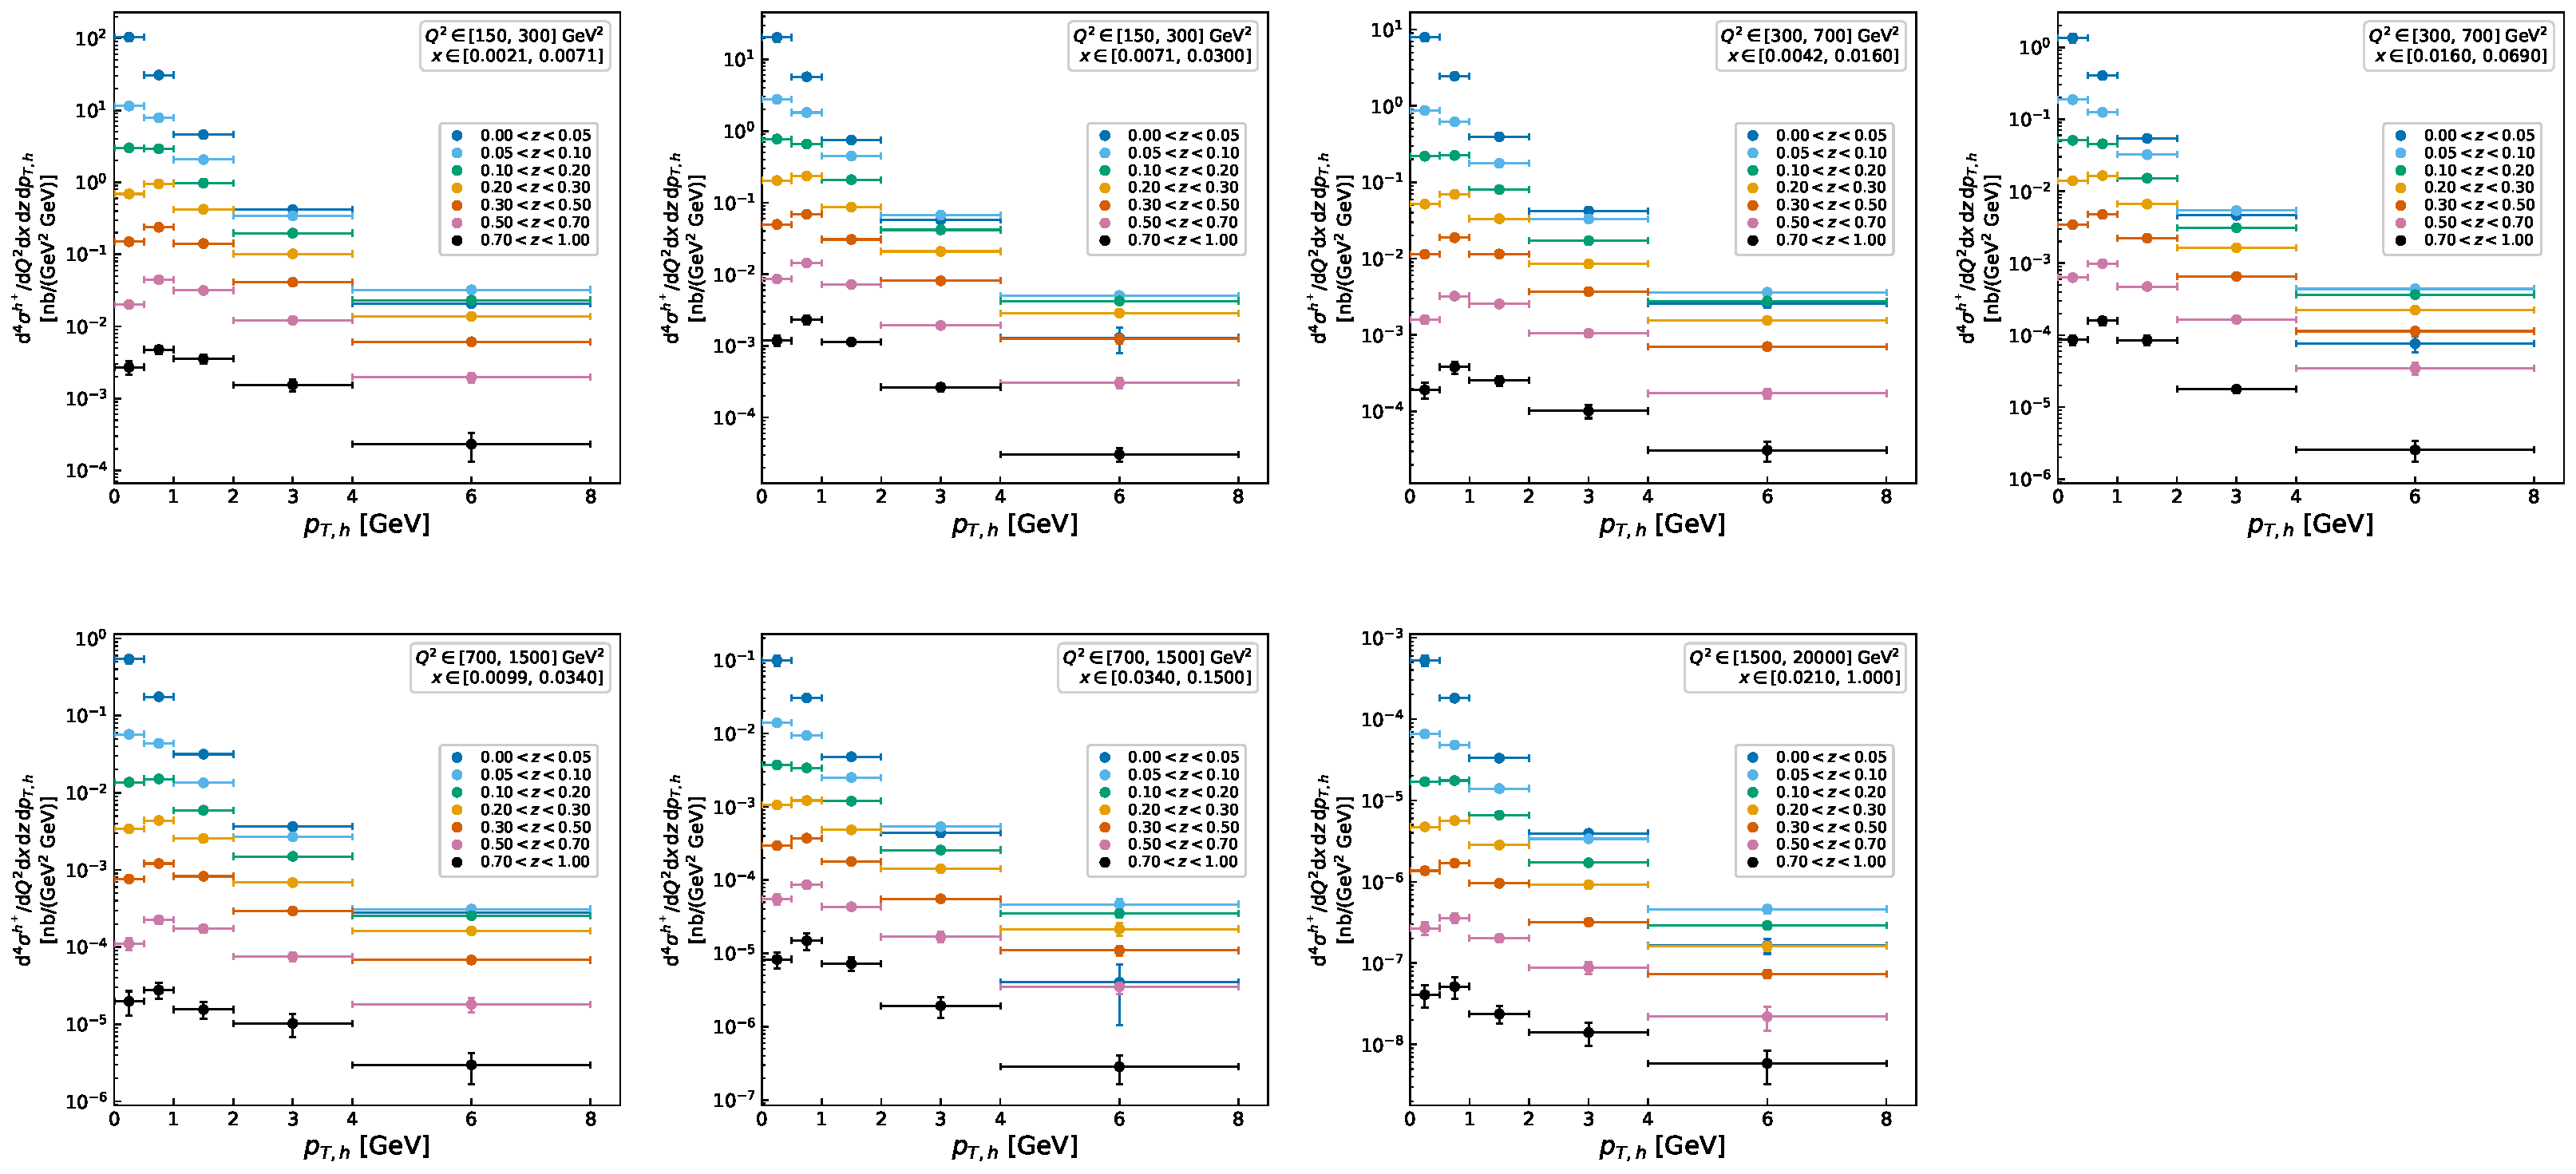
\includegraphics[width=0.98\textwidth,height=0.82\textheight,keepaspectratio]{figures/fig_results_xsec_density_born_cone_env100_7panel_hplus_z005_20261019.pdf}
  \caption{Born-level provisional cross-section density for $\hplus$
  from the iterative Bayesian unfolding, plotted as
  $\mathrm{d}^{4}\sigma/(\mathrm{d}\Qsq\,\mathrm{d}x\,
  \mathrm{d}z\,\mathrm{d}\pTh)$ in $\mathrm{nb}\,\GeV^{-3}$, at
  $\mathcal{L}_{\mathrm{data}}=351000.0~\mathrm{nb}^{-1}$.
  $C_{\mathrm{rad}}$ is applied per-bin post-unfold from the DJANGOH14
  (xFGen$<$0, EMPZ$>$45) table.  The points are the background-subtracted
  Born-level values of the superseded 2026-10-15 clean-release basis, which
  predates the OPT-A baseline promotion: the electron, V0, and low-$\Qsq$
  backgrounds are subtracted from the data vector before unfolding.  The band
  shows the quoted total systematic uncertainty of the frozen 2026-10-19
  budget, superseded as a quoting basis, whose median totals are
  $7.320288331169215\%$ for $\hplus$ and
  $7.637124635311324\%$ for $\hminus$.  This Born-level provisional figure
  carries internal-review status and is not physics-final.  Produced from the
  dated 2026-10-19 cross-section package
  \texttt{plots/cross\_sections/cone\_born\_7panel\_env100\_xcap\_2026-10-19/}.}
  \label{fig:results:release351-cone-xsec-density-hplus}
\end{figure}

\begin{figure}[p]
  \centering
  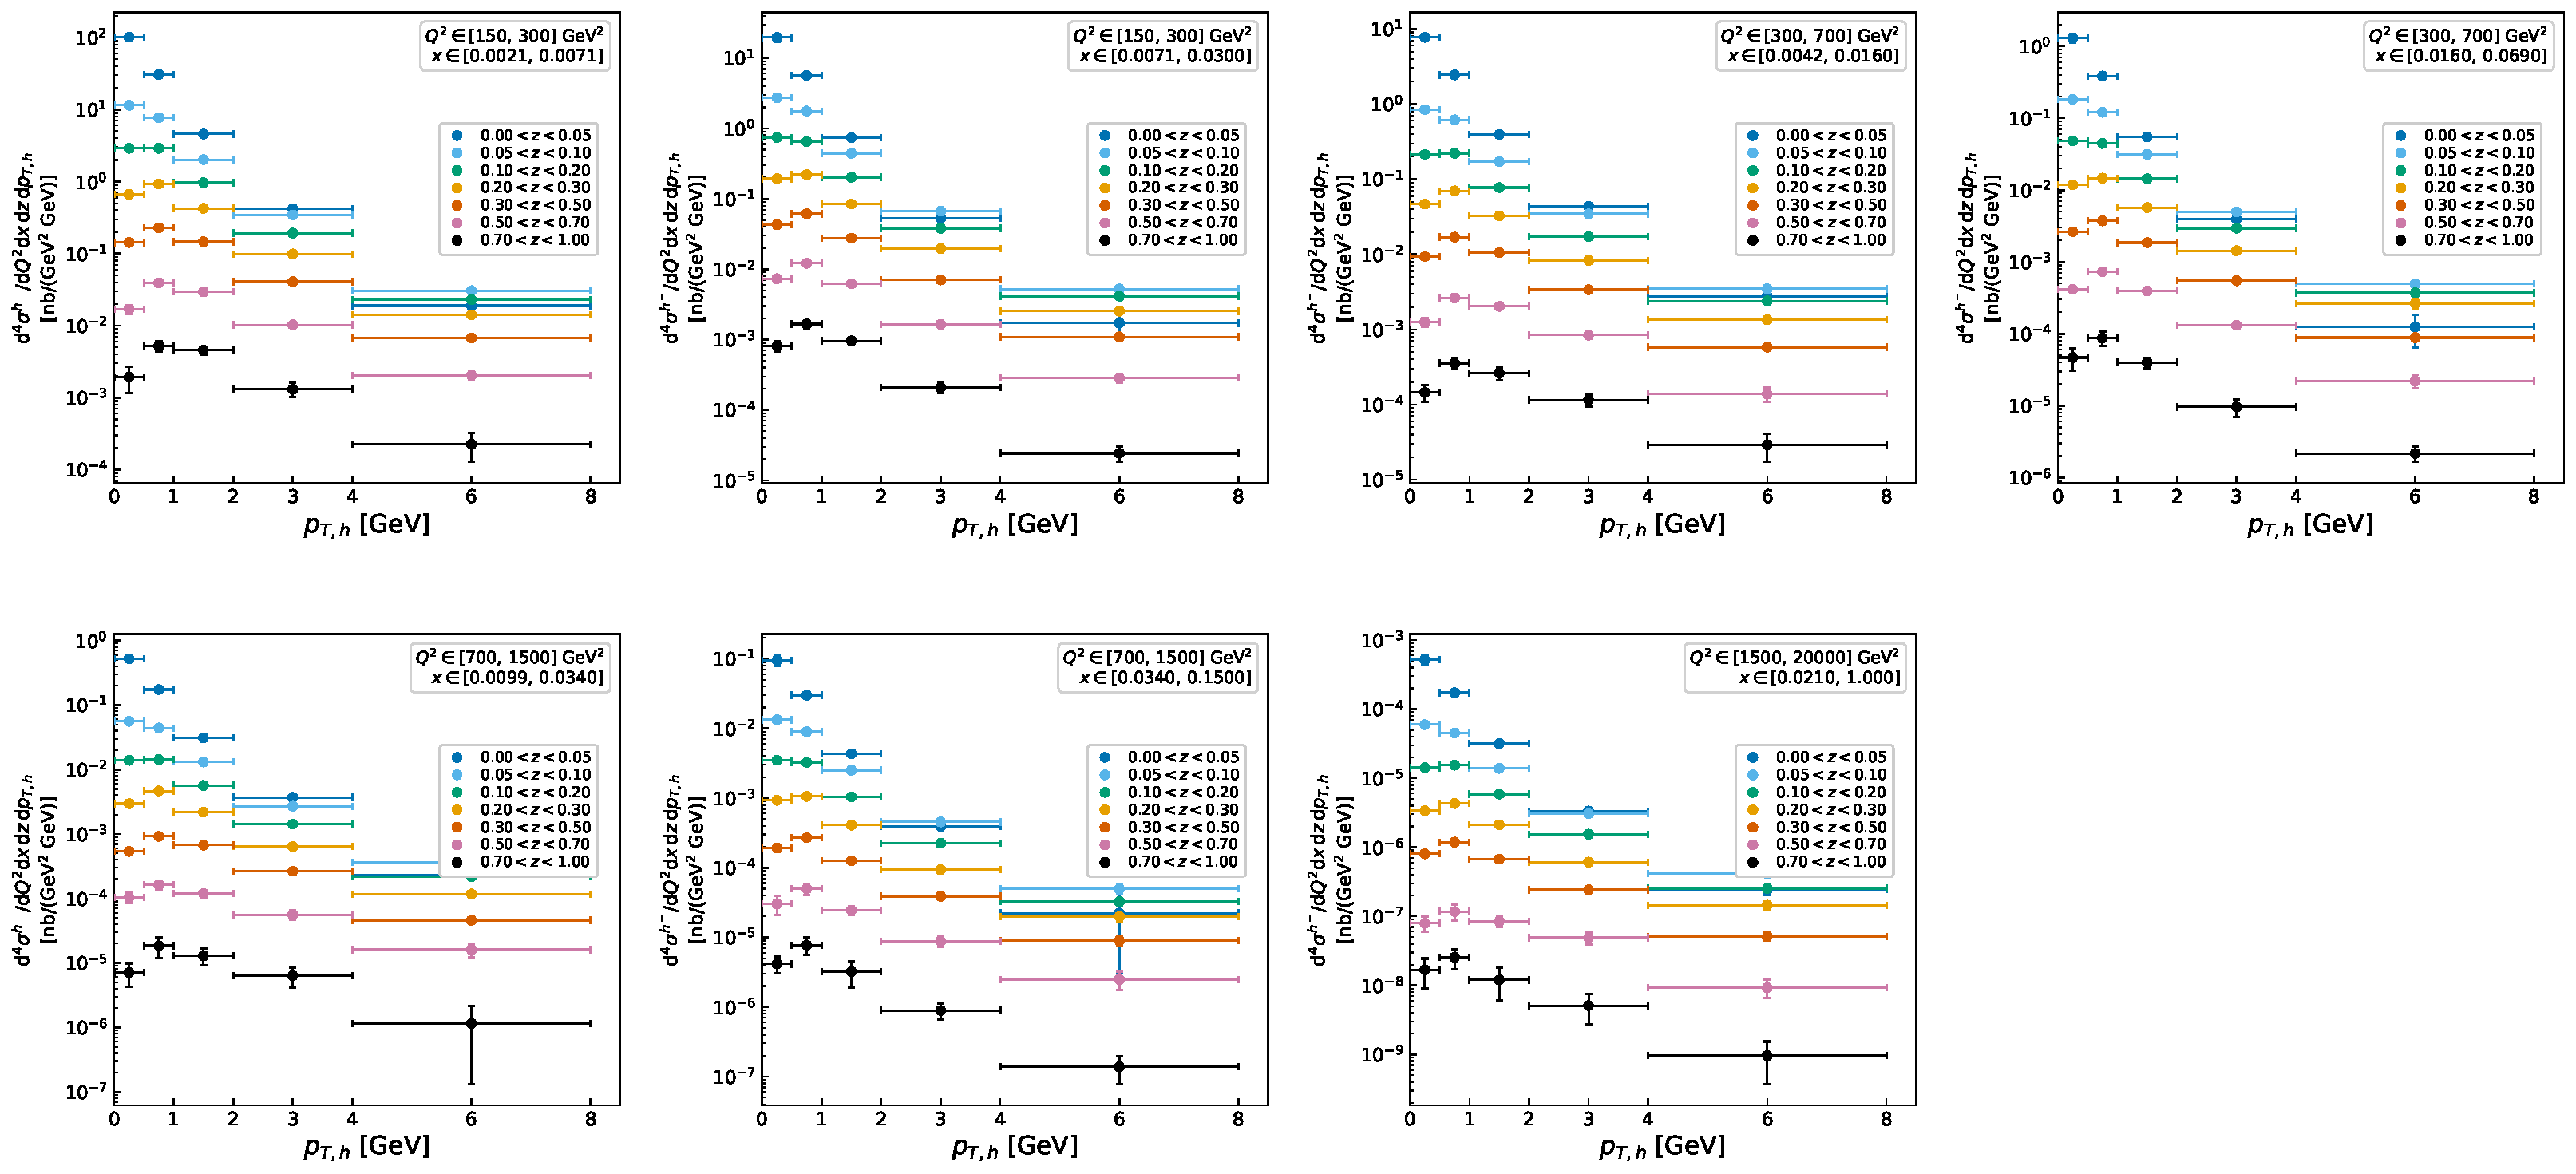
\includegraphics[width=0.98\textwidth,height=0.82\textheight,keepaspectratio]{figures/fig_results_xsec_density_born_cone_env100_7panel_hminus_z005_20261019.pdf}
  \caption{Born-level provisional cross-section density for $\hminus$
  from the iterative Bayesian unfolding, plotted as
  $\mathrm{d}^{4}\sigma/(\mathrm{d}\Qsq\,\mathrm{d}x\,
  \mathrm{d}z\,\mathrm{d}\pTh)$ in $\mathrm{nb}\,\GeV^{-3}$, at
  $\mathcal{L}_{\mathrm{data}}=351000.0~\mathrm{nb}^{-1}$.
  $C_{\mathrm{rad}}$ is applied per-bin post-unfold from the DJANGOH14
  (xFGen$<$0, EMPZ$>$45) table.  The points are the background-subtracted
  Born-level values of the superseded 2026-10-15 clean-release basis, which
  predates the OPT-A baseline promotion: the electron, V0, and low-$\Qsq$
  backgrounds are subtracted from the data vector before unfolding.  The band
  shows the quoted total systematic uncertainty of the frozen 2026-10-19
  budget, superseded as a quoting basis, whose median totals are
  $7.320288331169215\%$ for $\hplus$ and
  $7.637124635311324\%$ for $\hminus$.  This Born-level provisional figure
  carries internal-review status and is not physics-final.  Produced from the
  dated 2026-10-19 cross-section package
  \texttt{plots/cross\_sections/cone\_born\_7panel\_env100\_xcap\_2026-10-19/}.}
  \label{fig:results:release351-cone-xsec-density-hminus}
\end{figure}

\begin{figure}[p]
  \centering
  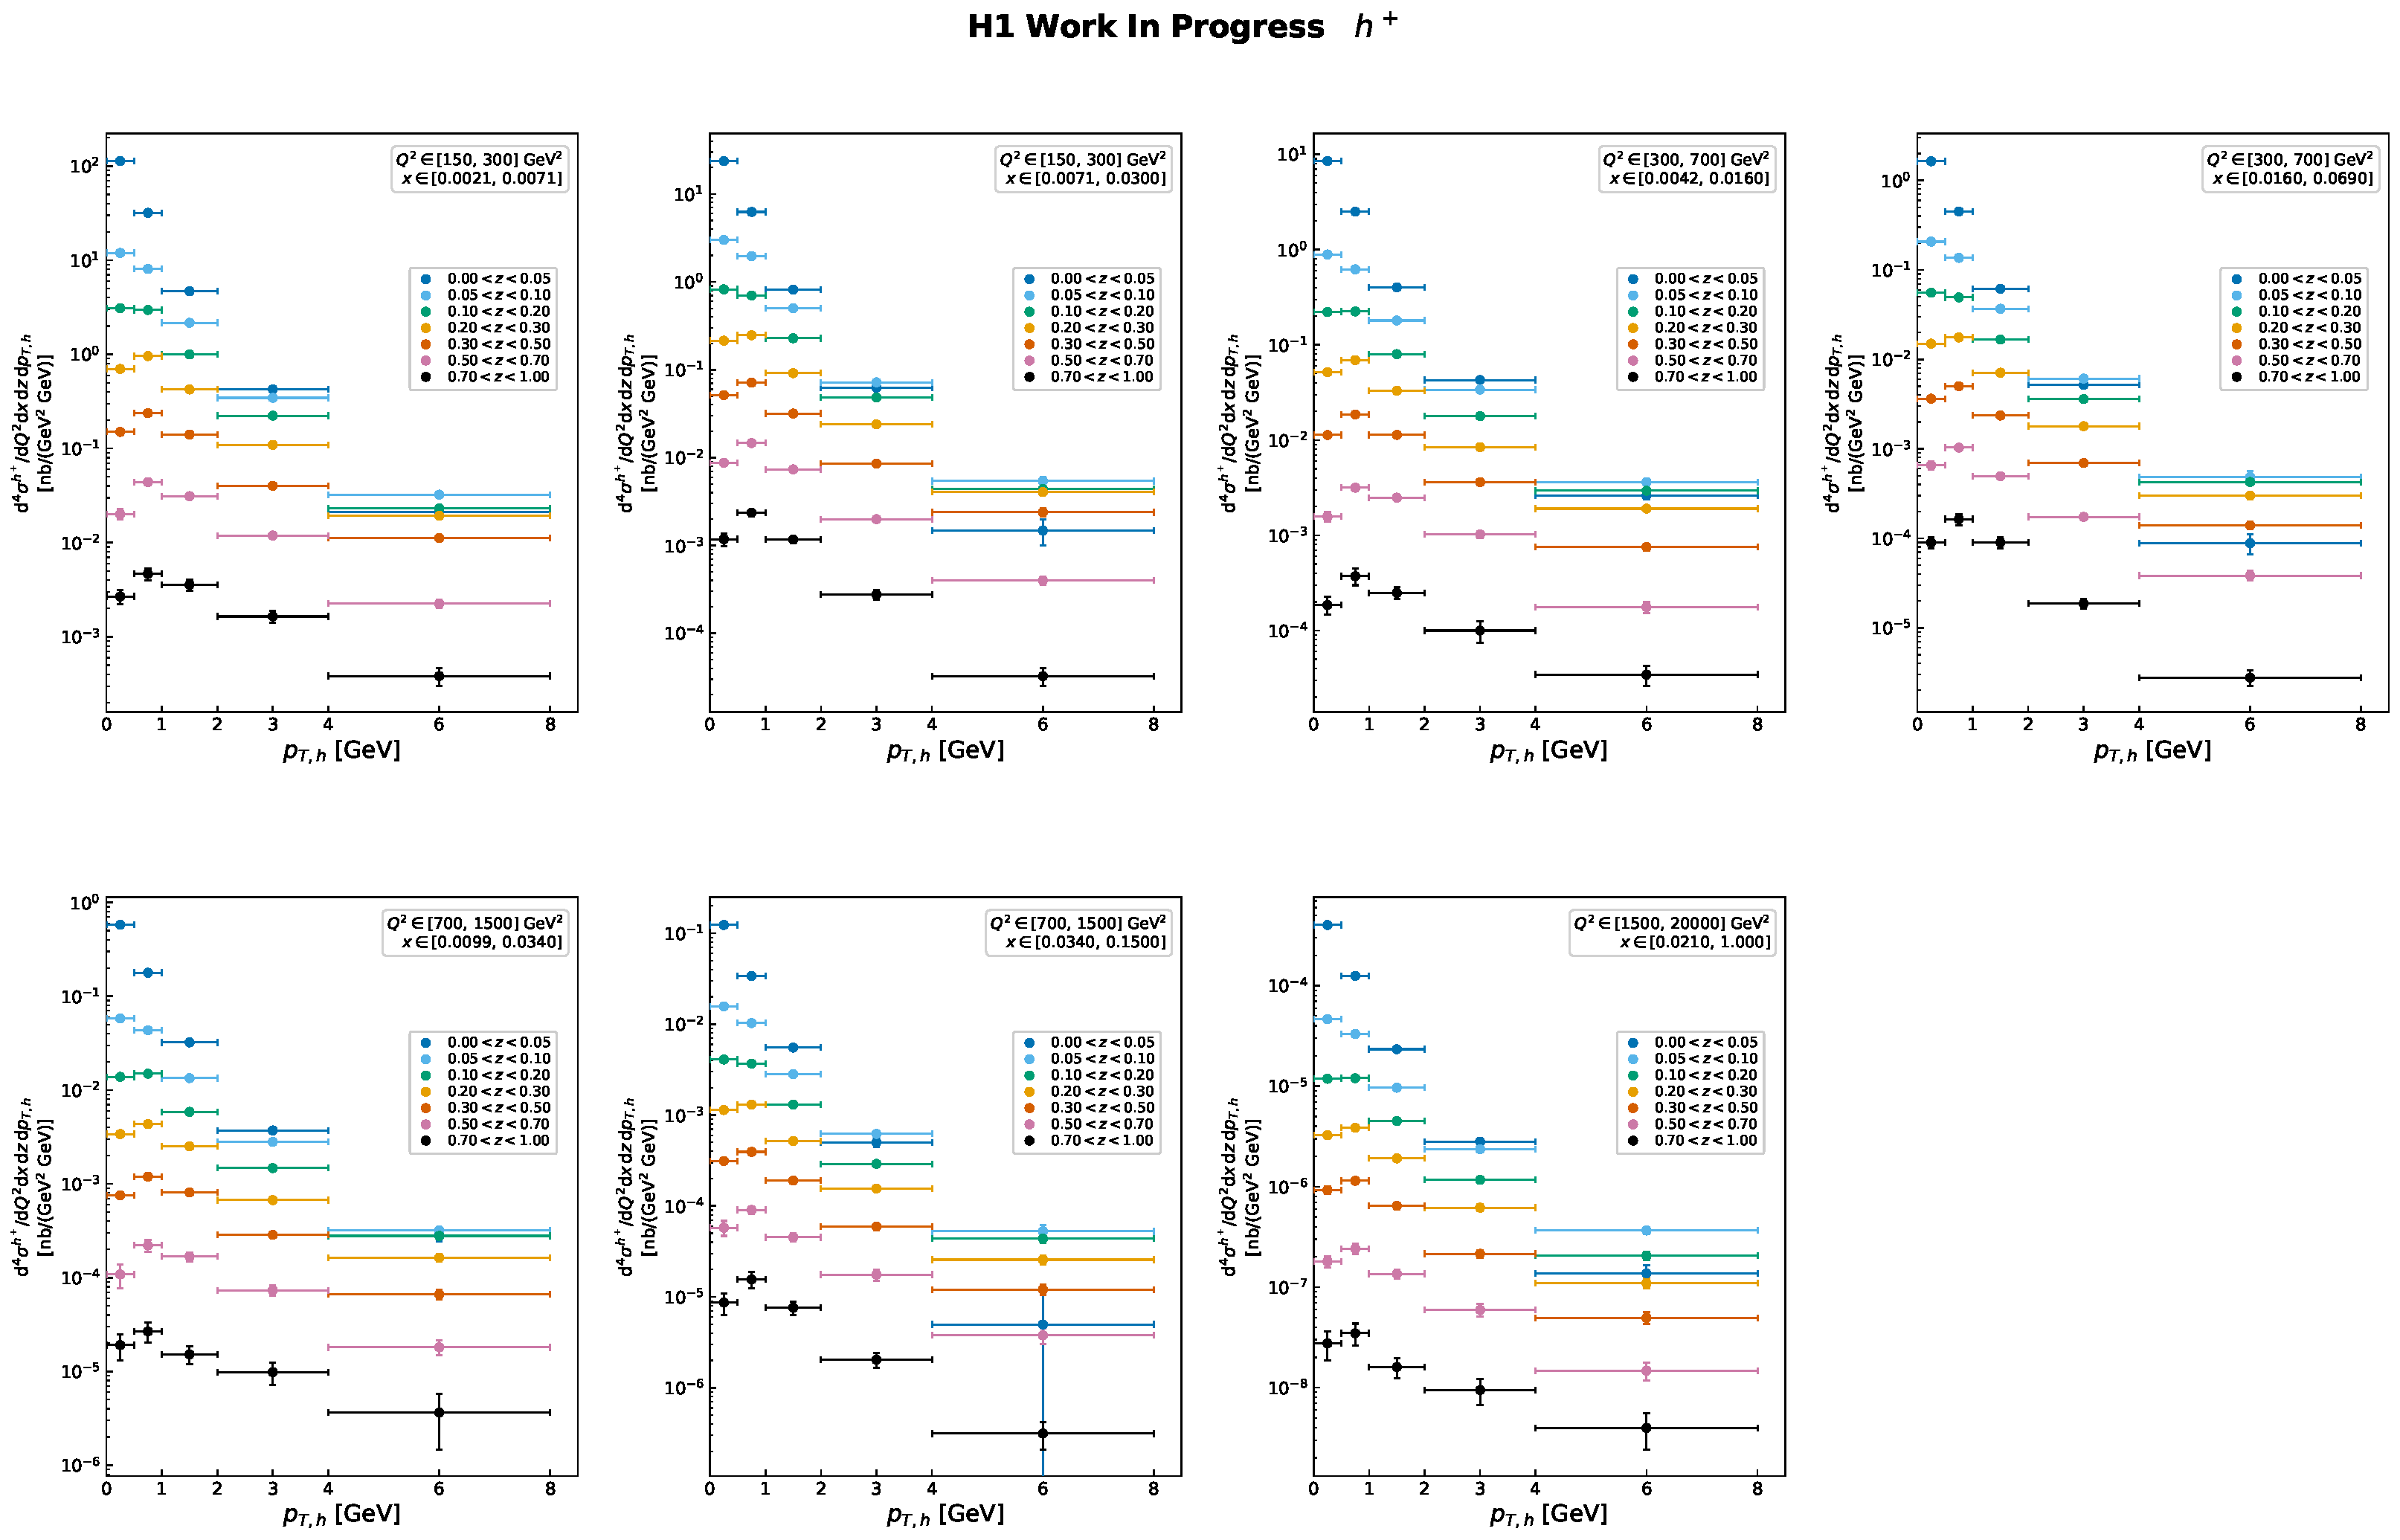
\includegraphics[width=0.98\textwidth,height=0.82\textheight,keepaspectratio]{figures/fig_results_xsec_density_born_crad13_coherentprior_7panel_hplus_z005_20261008.pdf}
  \caption{Born-level provisional cross-section density for $\hplus$ from the
  iterative Bayesian unfolding, on the superseded xFcut basis that predates
  the detector-interaction correction (2026-10-08 rendering), plotted as
  $\mathrm{d}^{4}\sigma/(\mathrm{d}\Qsq\,\mathrm{d}x\,
  \mathrm{d}z\,\mathrm{d}\pTh)$ in $\mathrm{nb}\,\GeV^{-3}$, with the
  response matrix's own generator-level distribution as the unfolding prior at
  $\mathcal{L}_{\mathrm{data}}=351000.0~\mathrm{nb}^{-1}$.
  $C_{\mathrm{rad}}$ is applied per-bin post-unfold from the DJANGOH14 xFcut
  (xFGen$<$0, EMPZ$>$45) table, and the vertical error bars show the full
  13-component systematic total, including the radiative components
  \texttt{c\_rad\_gen\_rel} and \texttt{c\_rad\_stat\_rel}.  The plot uses the
  canonical $|\eta_h|<1.6$ selection, with background handling by response
  fake-fraction subtraction only.  These values, which predate the
  detector-interaction correction, are superseded by the current cone-based
  figures above and are not physics-final.}
  \label{fig:results:release351-expanded-xsec-density-hplus}
\end{figure}

\begin{figure}[p]
  \centering
  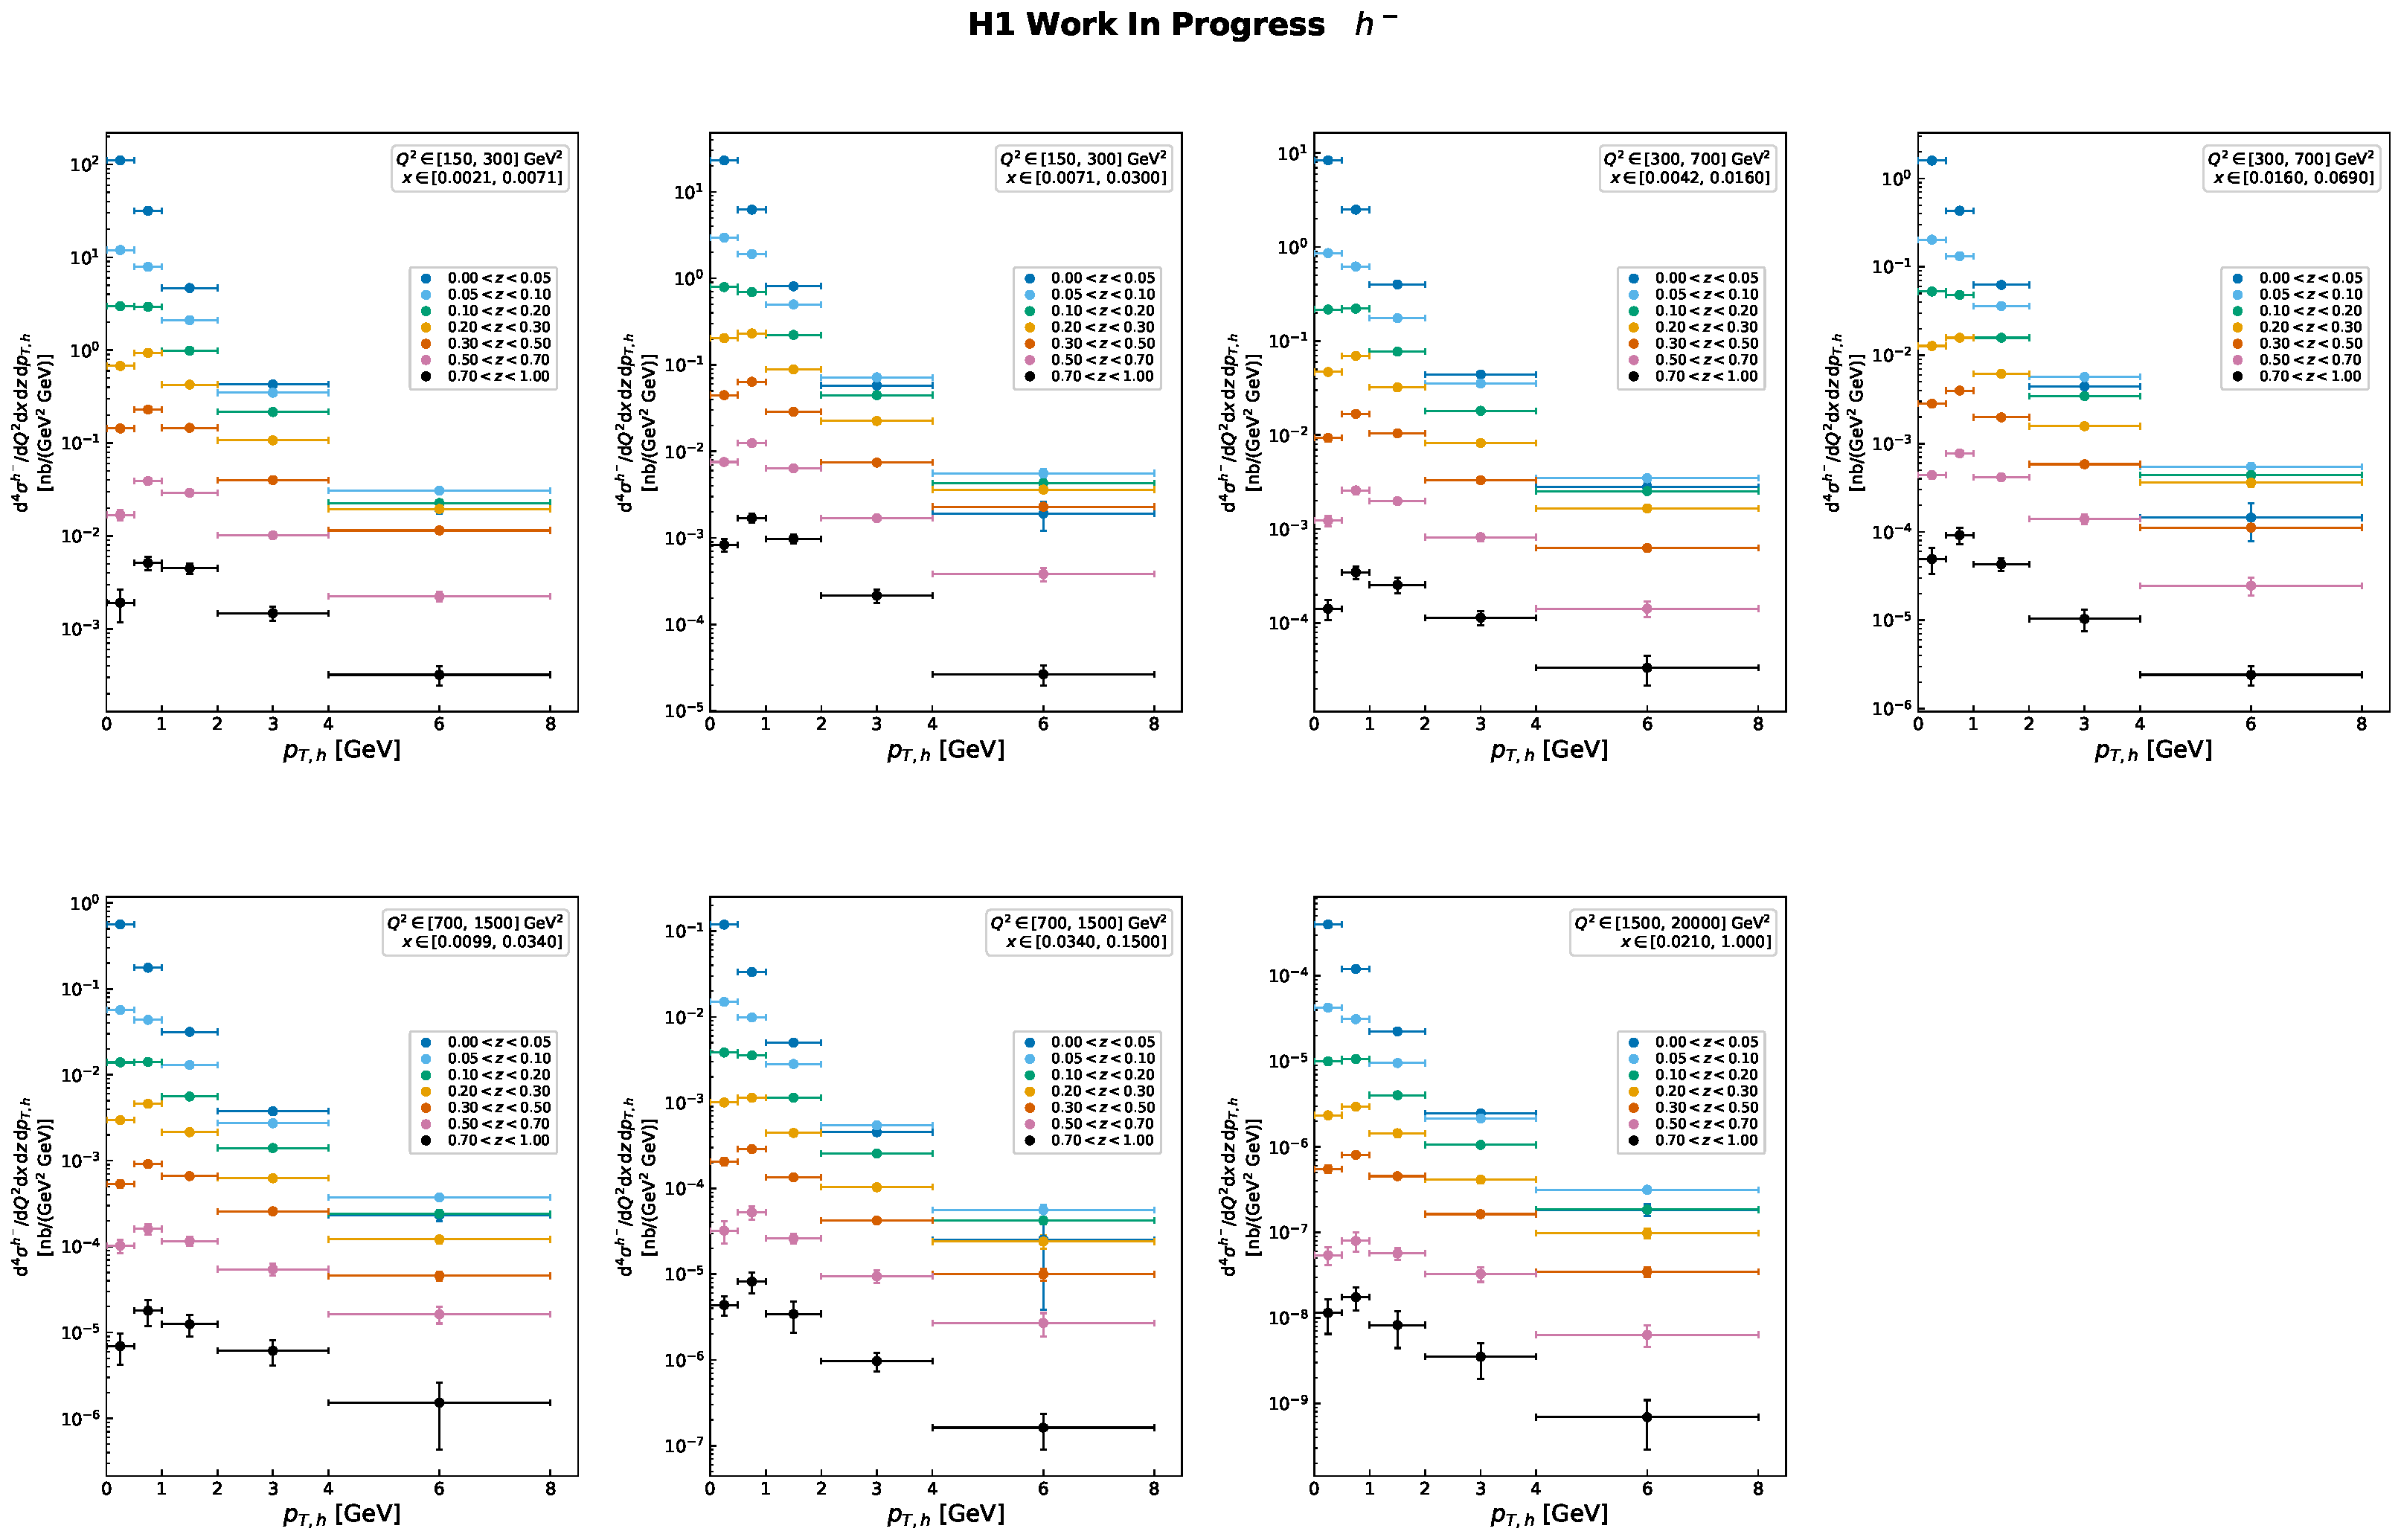
\includegraphics[width=0.98\textwidth,height=0.82\textheight,keepaspectratio]{figures/fig_results_xsec_density_born_crad13_coherentprior_7panel_hminus_z005_20261008.pdf}
  \caption{Born-level provisional cross-section density for $\hminus$ from the
  iterative Bayesian unfolding, on the superseded xFcut basis that predates
  the detector-interaction correction (2026-10-08 rendering), plotted as
  $\mathrm{d}^{4}\sigma/(\mathrm{d}\Qsq\,\mathrm{d}x\,
  \mathrm{d}z\,\mathrm{d}\pTh)$ in $\mathrm{nb}\,\GeV^{-3}$, with the
  response matrix's own generator-level distribution as the unfolding prior at
  $\mathcal{L}_{\mathrm{data}}=351000.0~\mathrm{nb}^{-1}$.
  $C_{\mathrm{rad}}$ is applied per-bin post-unfold from the DJANGOH14 xFcut
  (xFGen$<$0, EMPZ$>$45) table, and the vertical error bars show the full
  13-component systematic total, including the radiative components
  \texttt{c\_rad\_gen\_rel} and \texttt{c\_rad\_stat\_rel}.  The plot uses the
  canonical $|\eta_h|<1.6$ selection, with background handling by response
  fake-fraction subtraction only.  These values, which predate the
  detector-interaction correction, are superseded by the current cone-based
  figures above and are not physics-final.}
  \label{fig:results:release351-expanded-xsec-density-hminus}
\end{figure}

\subsection{Interpretation of Present Tables}
\label{sec:results:present-tables}

The release tables are suitable for validating the detector correction,
unfolding implementation, binning, and already-derived systematic components.
They are not yet the final multiplicity tables: the cross section now has the
per-bin post-unfold $C_{\mathrm{rad}}$ applied, with its uncertainty carried
as the radiative generator-difference and radiative-statistics components,
but no corrected inclusive DIS denominator is
available, so the multiplicity mapping remains pending. In particular, a
cross-section-ratio radiative diagnostic is not a substitute for the required
$M_{\mathrm{norad}}/M_{\mathrm{rad}}$ mapping.  The appendix tables of this
note are rendered on the current background-subtracted basis; their basis
statement is given in App.~\ref{app:born-xsec-tables}.

The release should therefore be circulated externally with the following status
qualification: detector, unfolding, background-subtraction, luminosity, and
radiative uncertainties are included, the radiative ones as the
generator-difference and statistical components; the five detector components
are full-chain single-sided shifts, with the HFS legs produced in the plus
direction only and their sign symmetry assumed, and the tracking-efficiency
component remains a data-side conservative shift; the electron, V0, and
low-$\Qsq$ backgrounds are subtracted before unfolding while the
detector-interaction class is removed response-internally, and the applied
$C_{\mathrm{rad}}$ is mixed-beam only; and the cut
variations are robustness checks rather than central results.  The frozen
systematic editions are superseded as a quoting basis and the budget is being
regenerated on the OPT-A nominal, so no per-bin uncertainty or total is final
until the regenerated budget passes review
(Sec.~\ref{sec:syst:budget-regeneration}).  No PID-separated
pion, kaon, or proton result is provided.

\subsection{Low-$\Qsq$ Companion Status}
\label{sec:results:lowq2-companion}

The low-$\Qsq$ charged-SIDIS analysis is a separate companion analysis covering
$5<\Qsq<100~\GeVsq$.  Its current publication-track headline is preliminary:
$\sigma_{\mathrm{total}}=463.9\pm5~\mathrm{(stat)}\pm47.9~\mathrm{(syst)}~\mathrm{nb}$
on the all-768-cell v3p3p1 TUnfold treatment, with $\sigma(\hplus)=233.3~\mathrm{nb}$,
$\sigma(\hminus)=230.7~\mathrm{nb}$, $\hplus/\hminus=1.011$, and
$\Ah=+0.00566$.  The low-$\Qsq$ result remains preliminary because several
systematic follow-ups are open, including validation of shifted-MC reuse at the
v3p3 fiducial, replacement of the analytic statistical quote by the bootstrap
value where appropriate, and additional checks of source summaries and
regularization details.  These low-$\Qsq$ numbers are not inputs to the
high-$\Qsq$ release.

% End of Results section.

% =============================================================================
%  Section: Summary and Conclusions
%  H1 Charged-Hadron SIDIS High-Q^2 Analysis Note
% =============================================================================
\section{Summary and Conclusions}
\label{sec:summary}

This note documents the inclusive charged-hadron SIDIS analysis at high
$\Qsq$ with H1.  The analysis uses the full four-period HERA-II data sample with
an integrated luminosity of $351~\pbinv$ and measures charge-separated inclusive
hadrons without PID splitting.  The truth-level charged-hadron convention for
response and acceptance work is limited to $\pi^{\pm}$, $K^{\pm}$, and $p/\bar p$.

The current analysis release has a validated 490-row published-bin contract,
with 245 $\hplus$ and 245 $\hminus$ bins, $N_{B,G}=245$ and $N_{B,R}=490$ per
charge setup, response shape $(491,246)$ per charge, data-vector length 980,
and a nominal four-iteration iterative Bayesian unfolding.  The selection
includes the $\alpha\ge0.2~\mathrm{rad}$ laboratory-frame scattered-electron
cone on the reconstructed legs, the unfolding prior is the response matrix's
own generator-level distribution, and the electron, V0, and low-$\Qsq$
background templates are subtracted from the data vector before unfolding.
Since the 2026-10-20 OPT-A baseline promotion, the response truth contract is
harmonized to the radiative correction
(Sec.~\ref{sec:unfolding:truth-contract}), and the OPT-A chain is the nominal
central-value release (Sec.~\ref{sec:results:z005-release}).
Detector, unfolding, tracking-efficiency,
luminosity, and radiative systematics have been propagated into the total
summary.  A
RooUnfoldBayes cross-check reproduces the in-house IBU central yields to
floating-point precision, with a maximum relative difference of
$2.6\times10^{-15}$ across 980 rows.

The radiative correction is applied to all released cross sections, which are
therefore Born-level, and its uncertainty is carried as two systematic
components; the application of the correction at the multiplicity level remains
open.  The principal remaining limitations are this multiplicity-level mapping
and the absence of a corrected inclusive DIS denominator.
The current release should therefore be treated as a validated working release,
not yet as a final physics multiplicity release.  The quoted total systematic
budget of the frozen 2026-10-19 edition combines twenty active uncertainty
terms on the background-subtracted basis, with median totals of
$7.320288331169215\%$ ($\hplus$) and $7.637124635311324\%$ ($\hminus$); the
frozen editions were computed on the superseded central values and are
superseded as a quoting basis, the budget is being regenerated on the OPT-A
nominal, and no per-bin uncertainty or total is final until the regenerated
budget passes review (Sec.~\ref{sec:syst:budget-regeneration}); its
principal background-related term is a fully correlated $\pm100\%$
normalization envelope on the subtracted electron and V0 content.  The five
detector-shift components are full-chain single-sided variations; the HFS legs
are produced in the plus direction only and their sign symmetry is assumed,
while the tracking-efficiency component remains a data-side conservative
shift.  The electron, V0, and low-$\Qsq$ backgrounds are subtracted from the
data vector before unfolding, while the detector-interaction removable class is
removed response-internally and must not be subtracted again externally.  The
applied $C_{\mathrm{rad}}$ is
mixed-beam only, and the release is not publication-grade: the exposure of the
simulated radiative samples is reconciled file by file, but the generator-log
cross-check is permanently blocked externally, and the correction tables
remain provisional.  The lab-$p_T$, $|\eta|$, and DCA variations provide
robustness checks rather than central results.

The low-$\Qsq$ charged-SIDIS companion analysis has a separate preliminary
v3p3p1 TUnfold publication-track result and open systematic follow-ups.  It is
kept separate from the high-$\Qsq$ analysis and is summarized here only to make
the charged-SIDIS status across the two regimes explicit.


% --- Appendices ------------------------------------------------------------
\begin{appendices}
\section{Reconstructed $\phi_h$ Distributions}
\label{app:reco-phih-alpha0p2}

This appendix collects the validated page-level reconstructed $\phi_h$ diagnostic plots with the reconstructed-level cut $\alpha(\mathrm{track},e) \ge 0.2\,\mathrm{rad}$. The plots are shown one page per $(\Qsq,x)$  bin for $\hplus$ and $\hminus$.

\clearpage

\begin{figure}[p]
  \centering
  \includegraphics[width=\textwidth,height=0.78\textheight,keepaspectratio]{figures/reco_phi_h_alpha0p2_pages/reco_phi_h_alpha0p2_distributions_hplus_page01.pdf}
  \caption{Reconstructed $\phi_h$ distributions for $\hplus$, $(\Qsq,x)$ bin $150 < \Qsq < 300\,\GeVsq$, $0.0021 < x < 0.0071$. }
  \label{fig:reco-phih-alpha0p2-dist-hplus-page01}
\end{figure}

\clearpage

\begin{figure}[p]
  \centering
  \includegraphics[width=\textwidth,height=0.78\textheight,keepaspectratio]{figures/reco_phi_h_alpha0p2_pages/reco_phi_h_alpha0p2_distributions_hplus_page02.pdf}
  \caption{Reconstructed $\phi_h$ distributions for $\hplus$, page 2, $(\Qsq,x)$  bin $150 < \Qsq < 300\,\GeVsq$, $0.0071 < x < 0.03$. }
  \label{fig:reco-phih-alpha0p2-dist-hplus-page02}
\end{figure}

\clearpage

\begin{figure}[p]
  \centering
  \includegraphics[width=\textwidth,height=0.78\textheight,keepaspectratio]{figures/reco_phi_h_alpha0p2_pages/reco_phi_h_alpha0p2_distributions_hplus_page03.pdf}
  \caption{Reconstructed $\phi_h$ distributions for $\hplus$, page 3, $(\Qsq,x)$  bin $300 < \Qsq < 700\,\GeVsq$, $0.0042 < x < 0.016$. }
  \label{fig:reco-phih-alpha0p2-dist-hplus-page03}
\end{figure}

\clearpage

\begin{figure}[p]
  \centering
  \includegraphics[width=\textwidth,height=0.78\textheight,keepaspectratio]{figures/reco_phi_h_alpha0p2_pages/reco_phi_h_alpha0p2_distributions_hplus_page04.pdf}
  \caption{Reconstructed $\phi_h$ distributions for $\hplus$, page 4, $(\Qsq,x)$  bin $300 < \Qsq < 700\,\GeVsq$, $0.016 < x < 0.069$. }
  \label{fig:reco-phih-alpha0p2-dist-hplus-page04}
\end{figure}

\clearpage

\begin{figure}[p]
  \centering
  \includegraphics[width=\textwidth,height=0.78\textheight,keepaspectratio]{figures/reco_phi_h_alpha0p2_pages/reco_phi_h_alpha0p2_distributions_hplus_page05.pdf}
  \caption{Reconstructed $\phi_h$ distributions for $\hplus$, page 5, $(\Qsq,x)$  bin $700 < \Qsq < 1500\,\GeVsq$, $0.0099 < x < 0.034$. }
  \label{fig:reco-phih-alpha0p2-dist-hplus-page05}
\end{figure}

\clearpage

\begin{figure}[p]
  \centering
  \includegraphics[width=\textwidth,height=0.78\textheight,keepaspectratio]{figures/reco_phi_h_alpha0p2_pages/reco_phi_h_alpha0p2_distributions_hplus_page06.pdf}
  \caption{Reconstructed $\phi_h$ distributions for $\hplus$, page 6, $(\Qsq,x)$  bin $700 < \Qsq < 1500\,\GeVsq$, $0.034 < x < 0.15$. }
  \label{fig:reco-phih-alpha0p2-dist-hplus-page06}
\end{figure}

\clearpage

\begin{figure}[p]
  \centering
  \includegraphics[width=\textwidth,height=0.78\textheight,keepaspectratio]{figures/reco_phi_h_alpha0p2_pages/reco_phi_h_alpha0p2_distributions_hplus_page07.pdf}
  \caption{Reconstructed $\phi_h$ distributions for $\hplus$, page 7, $(\Qsq,x)$  bin $1500 < \Qsq < 20000\,\GeVsq$, $0.021 < x < 1.0$. }
  \label{fig:reco-phih-alpha0p2-dist-hplus-page07}
\end{figure}

\clearpage

\begin{figure}[p]
  \centering
  \includegraphics[width=\textwidth,height=0.78\textheight,keepaspectratio]{figures/reco_phi_h_alpha0p2_pages/reco_phi_h_alpha0p2_distributions_hminus_page01.pdf}
  \caption{Reconstructed $\phi_h$ distributions for $\hminus$, page 1, $(\Qsq,x)$  bin $150 < \Qsq < 300\,\GeVsq$, $0.0021 < x < 0.0071$. }
  \label{fig:reco-phih-alpha0p2-dist-hminus-page01}
\end{figure}

\clearpage

\begin{figure}[p]
  \centering
  \includegraphics[width=\textwidth,height=0.78\textheight,keepaspectratio]{figures/reco_phi_h_alpha0p2_pages/reco_phi_h_alpha0p2_distributions_hminus_page02.pdf}
  \caption{Reconstructed $\phi_h$ distributions for $\hminus$, page 2, $(\Qsq,x)$  bin $150 < \Qsq < 300\,\GeVsq$, $0.0071 < x < 0.03$. }
  \label{fig:reco-phih-alpha0p2-dist-hminus-page02}
\end{figure}

\clearpage

\begin{figure}[p]
  \centering
  \includegraphics[width=\textwidth,height=0.78\textheight,keepaspectratio]{figures/reco_phi_h_alpha0p2_pages/reco_phi_h_alpha0p2_distributions_hminus_page03.pdf}
  \caption{Reconstructed $\phi_h$ distributions for $\hminus$, page 3, $(\Qsq,x)$  bin $300 < \Qsq < 700\,\GeVsq$, $0.0042 < x < 0.016$. }
  \label{fig:reco-phih-alpha0p2-dist-hminus-page03}
\end{figure}

\clearpage

\begin{figure}[p]
  \centering
  \includegraphics[width=\textwidth,height=0.78\textheight,keepaspectratio]{figures/reco_phi_h_alpha0p2_pages/reco_phi_h_alpha0p2_distributions_hminus_page04.pdf}
  \caption{Reconstructed $\phi_h$ distributions for $\hminus$, page 4, $(\Qsq,x)$  bin $300 < \Qsq < 700\,\GeVsq$, $0.016 < x < 0.069$. }
  \label{fig:reco-phih-alpha0p2-dist-hminus-page04}
\end{figure}

\clearpage

\begin{figure}[p]
  \centering
  \includegraphics[width=\textwidth,height=0.78\textheight,keepaspectratio]{figures/reco_phi_h_alpha0p2_pages/reco_phi_h_alpha0p2_distributions_hminus_page05.pdf}
  \caption{Reconstructed $\phi_h$ distributions for $\hminus$, page 5, $(\Qsq,x)$  bin $700 < \Qsq < 1500\,\GeVsq$, $0.0099 < x < 0.034$. }
  \label{fig:reco-phih-alpha0p2-dist-hminus-page05}
\end{figure}

\clearpage

\begin{figure}[p]
  \centering
  \includegraphics[width=\textwidth,height=0.78\textheight,keepaspectratio]{figures/reco_phi_h_alpha0p2_pages/reco_phi_h_alpha0p2_distributions_hminus_page06.pdf}
  \caption{Reconstructed $\phi_h$ distributions for $\hminus$, page 6, $(\Qsq,x)$  bin $700 < \Qsq < 1500\,\GeVsq$, $0.034 < x < 0.15$. }
  \label{fig:reco-phih-alpha0p2-dist-hminus-page06}
\end{figure}

\clearpage

\begin{figure}[p]
  \centering
  \includegraphics[width=\textwidth,height=0.78\textheight,keepaspectratio]{figures/reco_phi_h_alpha0p2_pages/reco_phi_h_alpha0p2_distributions_hminus_page07.pdf}
  \caption{Reconstructed $\phi_h$ distributions for $\hminus$, page 7, $(\Qsq,x)$  bin $1500 < \Qsq < 20000\,\GeVsq$, $0.021 < x < 1.0$. }
  \label{fig:reco-phih-alpha0p2-dist-hminus-page07}
\end{figure}

\clearpage

\begin{figure}[p]
  \centering
  \includegraphics[width=\textwidth,height=0.78\textheight,keepaspectratio]{figures/reco_phi_h_alpha0p2_pages/reco_phi_h_alpha0p2_ratios_hplus_page01.pdf}
  \caption{Reconstructed $\phi_h$ MC/data ratios for $\hplus$, page 1, $(\Qsq,x)$  bin $150 < \Qsq < 300\,\GeVsq$, $0.0021 < x < 0.0071$.  Ratios are DJANGOH/data and RAPGAP/data.}
  \label{fig:reco-phih-alpha0p2-ratio-hplus-page01}
\end{figure}

\clearpage

\begin{figure}[p]
  \centering
  \includegraphics[width=\textwidth,height=0.78\textheight,keepaspectratio]{figures/reco_phi_h_alpha0p2_pages/reco_phi_h_alpha0p2_ratios_hplus_page02.pdf}
  \caption{Reconstructed $\phi_h$ MC/data ratios for $\hplus$, page 2, $(\Qsq,x)$  bin $150 < \Qsq < 300\,\GeVsq$, $0.0071 < x < 0.03$.  Ratios are DJANGOH/data and RAPGAP/data.}
  \label{fig:reco-phih-alpha0p2-ratio-hplus-page02}
\end{figure}

\clearpage

\begin{figure}[p]
  \centering
  \includegraphics[width=\textwidth,height=0.78\textheight,keepaspectratio]{figures/reco_phi_h_alpha0p2_pages/reco_phi_h_alpha0p2_ratios_hplus_page03.pdf}
  \caption{Reconstructed $\phi_h$ MC/data ratios for $\hplus$, page 3, $(\Qsq,x)$  bin $300 < \Qsq < 700\,\GeVsq$, $0.0042 < x < 0.016$.  Ratios are DJANGOH/data and RAPGAP/data.}
  \label{fig:reco-phih-alpha0p2-ratio-hplus-page03}
\end{figure}

\clearpage

\begin{figure}[p]
  \centering
  \includegraphics[width=\textwidth,height=0.78\textheight,keepaspectratio]{figures/reco_phi_h_alpha0p2_pages/reco_phi_h_alpha0p2_ratios_hplus_page04.pdf}
  \caption{Reconstructed $\phi_h$ MC/data ratios for $\hplus$, page 4, $(\Qsq,x)$  bin $300 < \Qsq < 700\,\GeVsq$, $0.016 < x < 0.069$.  Ratios are DJANGOH/data and RAPGAP/data.}
  \label{fig:reco-phih-alpha0p2-ratio-hplus-page04}
\end{figure}

\clearpage

\begin{figure}[p]
  \centering
  \includegraphics[width=\textwidth,height=0.78\textheight,keepaspectratio]{figures/reco_phi_h_alpha0p2_pages/reco_phi_h_alpha0p2_ratios_hplus_page05.pdf}
  \caption{Reconstructed $\phi_h$ MC/data ratios for $\hplus$, page 5, $(\Qsq,x)$  bin $700 < \Qsq < 1500\,\GeVsq$, $0.0099 < x < 0.034$.  Ratios are DJANGOH/data and RAPGAP/data.}
  \label{fig:reco-phih-alpha0p2-ratio-hplus-page05}
\end{figure}

\clearpage

\begin{figure}[p]
  \centering
  \includegraphics[width=\textwidth,height=0.78\textheight,keepaspectratio]{figures/reco_phi_h_alpha0p2_pages/reco_phi_h_alpha0p2_ratios_hplus_page06.pdf}
  \caption{Reconstructed $\phi_h$ MC/data ratios for $\hplus$, page 6, $(\Qsq,x)$  bin $700 < \Qsq < 1500\,\GeVsq$, $0.034 < x < 0.15$.  Ratios are DJANGOH/data and RAPGAP/data.}
  \label{fig:reco-phih-alpha0p2-ratio-hplus-page06}
\end{figure}

\clearpage

\begin{figure}[p]
  \centering
  \includegraphics[width=\textwidth,height=0.78\textheight,keepaspectratio]{figures/reco_phi_h_alpha0p2_pages/reco_phi_h_alpha0p2_ratios_hplus_page07.pdf}
  \caption{Reconstructed $\phi_h$ MC/data ratios for $\hplus$, page 7, $(\Qsq,x)$  bin $1500 < \Qsq < 20000\,\GeVsq$, $0.021 < x < 1.0$.  Ratios are DJANGOH/data and RAPGAP/data.}
  \label{fig:reco-phih-alpha0p2-ratio-hplus-page07}
\end{figure}

\clearpage

\begin{figure}[p]
  \centering
  \includegraphics[width=\textwidth,height=0.78\textheight,keepaspectratio]{figures/reco_phi_h_alpha0p2_pages/reco_phi_h_alpha0p2_ratios_hminus_page01.pdf}
  \caption{Reconstructed $\phi_h$ MC/data ratios for $\hminus$, page 1, $(\Qsq,x)$  bin $150 < \Qsq < 300\,\GeVsq$, $0.0021 < x < 0.0071$.  Ratios are DJANGOH/data and RAPGAP/data.}
  \label{fig:reco-phih-alpha0p2-ratio-hminus-page01}
\end{figure}

\clearpage

\begin{figure}[p]
  \centering
  \includegraphics[width=\textwidth,height=0.78\textheight,keepaspectratio]{figures/reco_phi_h_alpha0p2_pages/reco_phi_h_alpha0p2_ratios_hminus_page02.pdf}
  \caption{Reconstructed $\phi_h$ MC/data ratios for $\hminus$, page 2, $(\Qsq,x)$  bin $150 < \Qsq < 300\,\GeVsq$, $0.0071 < x < 0.03$.  Ratios are DJANGOH/data and RAPGAP/data.}
  \label{fig:reco-phih-alpha0p2-ratio-hminus-page02}
\end{figure}

\clearpage

\begin{figure}[p]
  \centering
  \includegraphics[width=\textwidth,height=0.78\textheight,keepaspectratio]{figures/reco_phi_h_alpha0p2_pages/reco_phi_h_alpha0p2_ratios_hminus_page03.pdf}
  \caption{Reconstructed $\phi_h$ MC/data ratios for $\hminus$, page 3, $(\Qsq,x)$  bin $300 < \Qsq < 700\,\GeVsq$, $0.0042 < x < 0.016$.  Ratios are DJANGOH/data and RAPGAP/data.}
  \label{fig:reco-phih-alpha0p2-ratio-hminus-page03}
\end{figure}

\clearpage

\begin{figure}[p]
  \centering
  \includegraphics[width=\textwidth,height=0.78\textheight,keepaspectratio]{figures/reco_phi_h_alpha0p2_pages/reco_phi_h_alpha0p2_ratios_hminus_page04.pdf}
  \caption{Reconstructed $\phi_h$ MC/data ratios for $\hminus$, page 4, $(\Qsq,x)$  bin $300 < \Qsq < 700\,\GeVsq$, $0.016 < x < 0.069$.  Ratios are DJANGOH/data and RAPGAP/data.}
  \label{fig:reco-phih-alpha0p2-ratio-hminus-page04}
\end{figure}

\clearpage

\begin{figure}[p]
  \centering
  \includegraphics[width=\textwidth,height=0.78\textheight,keepaspectratio]{figures/reco_phi_h_alpha0p2_pages/reco_phi_h_alpha0p2_ratios_hminus_page05.pdf}
  \caption{Reconstructed $\phi_h$ MC/data ratios for $\hminus$, page 5, $(\Qsq,x)$  bin $700 < \Qsq < 1500\,\GeVsq$, $0.0099 < x < 0.034$.  Ratios are DJANGOH/data and RAPGAP/data.}
  \label{fig:reco-phih-alpha0p2-ratio-hminus-page05}
\end{figure}

\clearpage

\begin{figure}[p]
  \centering
  \includegraphics[width=\textwidth,height=0.78\textheight,keepaspectratio]{figures/reco_phi_h_alpha0p2_pages/reco_phi_h_alpha0p2_ratios_hminus_page06.pdf}
  \caption{Reconstructed $\phi_h$ MC/data ratios for $\hminus$, page 6, $(\Qsq,x)$  bin $700 < \Qsq < 1500\,\GeVsq$, $0.034 < x < 0.15$.  Ratios are DJANGOH/data and RAPGAP/data.}
  \label{fig:reco-phih-alpha0p2-ratio-hminus-page06}
\end{figure}

\clearpage

\begin{figure}[p]
  \centering
  \includegraphics[width=\textwidth,height=0.78\textheight,keepaspectratio]{figures/reco_phi_h_alpha0p2_pages/reco_phi_h_alpha0p2_ratios_hminus_page07.pdf}
  \caption{Reconstructed $\phi_h$ MC/data ratios for $\hminus$, page 7, $(\Qsq,x)$  bin $1500 < \Qsq < 20000\,\GeVsq$, $0.021 < x < 1.0$.  Ratios are DJANGOH/data and RAPGAP/data.}
  \label{fig:reco-phih-alpha0p2-ratio-hminus-page07}
\end{figure}

\clearpage

\section{Generator-Level $\phi_h$ Distributions}
\label{app:gen-phih-radnonrad}

This appendix collects the generator-level $\phi_h$ distributions from the DJANGOH14 and RAPGAP31 samples, with the radiative and non-radiative samples of each generator overlaid, one figure per truth $(\Qsq,x)$ cell, first for $\hplus$ (cells 1--7) and then for $\hminus$ (cells 1--7). These are uncorrected generator-level (truth) Monte Carlo distributions with no detector simulation and no acceptance correction, and the QED radiative correction $C_{\mathrm{rad}}$ is not applied; the product is an internal diagnostic, not a measurement. Each figure shows a grid of 7 $z$ rows ($0$--$0.05$, $0.05$--$0.1$, $0.1$--$0.2$, $0.2$--$0.3$, $0.3$--$0.5$, $0.5$--$0.7$, $0.7$--$1.0$) by 5 $\pTh$ columns ($0$--$0.5$, $0.5$--$1$, $1$--$2$, $2$--$4$, $4$--$8~\GeV$); $\phi_h$ is computed in the $\gamma^{*}p$ center-of-mass frame, Trento convention, on $[-\pi,\pi]$. The per-panel azimuthal moments reach $|\langle\cos\phi_h\rangle| \sim 0.4$, while the global averages are much smaller.

\clearpage

\begin{figure}[p]
  \centering
  \includegraphics[width=\textwidth,height=0.78\textheight,keepaspectratio]{figures/gen_phi_h_radnonrad_pages/gen_phi_h_radnonrad_distributions_hplus_cell01.pdf}
  \caption{DJANGOH and RAPGAP generator-level $\phi_h$ distributions for $150 < \Qsq < 300\,\GeVsq$, $0.0021 < x < 0.0071$, $\hplus$, cell 1.}
  \label{fig:gen-phih-radnonrad-dist-hplus-cell01}
\end{figure}

\clearpage

\begin{figure}[p]
  \centering
  \includegraphics[width=\textwidth,height=0.78\textheight,keepaspectratio]{figures/gen_phi_h_radnonrad_pages/gen_phi_h_radnonrad_distributions_hplus_cell02.pdf}
  \caption{DJANGOH and RAPGAP generator-level $\phi_h$ distributions for $150 < \Qsq < 300\,\GeVsq$, $0.0071 < x < 0.03$, $\hplus$, cell 2.}
  \label{fig:gen-phih-radnonrad-dist-hplus-cell02}
\end{figure}

\clearpage

\begin{figure}[p]
  \centering
  \includegraphics[width=\textwidth,height=0.78\textheight,keepaspectratio]{figures/gen_phi_h_radnonrad_pages/gen_phi_h_radnonrad_distributions_hplus_cell03.pdf}
  \caption{DJANGOH and RAPGAP generator-level $\phi_h$ distributions for $300 < \Qsq < 700\,\GeVsq$, $0.0042 < x < 0.016$, $\hplus$, cell 3.}
  \label{fig:gen-phih-radnonrad-dist-hplus-cell03}
\end{figure}

\clearpage

\begin{figure}[p]
  \centering
  \includegraphics[width=\textwidth,height=0.78\textheight,keepaspectratio]{figures/gen_phi_h_radnonrad_pages/gen_phi_h_radnonrad_distributions_hplus_cell04.pdf}
  \caption{DJANGOH and RAPGAP generator-level $\phi_h$ distributions for $300 < \Qsq < 700\,\GeVsq$, $0.016 < x < 0.069$, $\hplus$, cell 4.}
  \label{fig:gen-phih-radnonrad-dist-hplus-cell04}
\end{figure}

\clearpage

\begin{figure}[p]
  \centering
  \includegraphics[width=\textwidth,height=0.78\textheight,keepaspectratio]{figures/gen_phi_h_radnonrad_pages/gen_phi_h_radnonrad_distributions_hplus_cell05.pdf}
  \caption{DJANGOH and RAPGAP generator-level $\phi_h$ distributions for $700 < \Qsq < 1500\,\GeVsq$, $0.0099 < x < 0.034$, $\hplus$, cell 5.}
  \label{fig:gen-phih-radnonrad-dist-hplus-cell05}
\end{figure}

\clearpage

\begin{figure}[p]
  \centering
  \includegraphics[width=\textwidth,height=0.78\textheight,keepaspectratio]{figures/gen_phi_h_radnonrad_pages/gen_phi_h_radnonrad_distributions_hplus_cell06.pdf}
  \caption{DJANGOH and RAPGAP generator-level $\phi_h$ distributions for $700 < \Qsq < 1500\,\GeVsq$, $0.034 < x < 0.15$, $\hplus$, cell 6.}
  \label{fig:gen-phih-radnonrad-dist-hplus-cell06}
\end{figure}

\clearpage

\begin{figure}[p]
  \centering
  \includegraphics[width=\textwidth,height=0.78\textheight,keepaspectratio]{figures/gen_phi_h_radnonrad_pages/gen_phi_h_radnonrad_distributions_hplus_cell07.pdf}
  \caption{DJANGOH and RAPGAP generator-level $\phi_h$ distributions for $1500 < \Qsq < 20000\,\GeVsq$, $0.021 < x < 1.0$, $\hplus$, cell 7.}
  \label{fig:gen-phih-radnonrad-dist-hplus-cell07}
\end{figure}

\clearpage

\begin{figure}[p]
  \centering
  \includegraphics[width=\textwidth,height=0.78\textheight,keepaspectratio]{figures/gen_phi_h_radnonrad_pages/gen_phi_h_radnonrad_distributions_hminus_cell01.pdf}
  \caption{DJANGOH and RAPGAP generator-level $\phi_h$ distributions for $150 < \Qsq < 300\,\GeVsq$, $0.0021 < x < 0.0071$, $\hminus$, cell 1.}
  \label{fig:gen-phih-radnonrad-dist-hminus-cell01}
\end{figure}

\clearpage

\begin{figure}[p]
  \centering
  \includegraphics[width=\textwidth,height=0.78\textheight,keepaspectratio]{figures/gen_phi_h_radnonrad_pages/gen_phi_h_radnonrad_distributions_hminus_cell02.pdf}
  \caption{DJANGOH and RAPGAP generator-level $\phi_h$ distributions for $150 < \Qsq < 300\,\GeVsq$, $0.0071 < x < 0.03$, $\hminus$, cell 2.}
  \label{fig:gen-phih-radnonrad-dist-hminus-cell02}
\end{figure}

\clearpage

\begin{figure}[p]
  \centering
  \includegraphics[width=\textwidth,height=0.78\textheight,keepaspectratio]{figures/gen_phi_h_radnonrad_pages/gen_phi_h_radnonrad_distributions_hminus_cell03.pdf}
  \caption{DJANGOH and RAPGAP generator-level $\phi_h$ distributions for $300 < \Qsq < 700\,\GeVsq$, $0.0042 < x < 0.016$, $\hminus$, cell 3.}
  \label{fig:gen-phih-radnonrad-dist-hminus-cell03}
\end{figure}

\clearpage

\begin{figure}[p]
  \centering
  \includegraphics[width=\textwidth,height=0.78\textheight,keepaspectratio]{figures/gen_phi_h_radnonrad_pages/gen_phi_h_radnonrad_distributions_hminus_cell04.pdf}
  \caption{DJANGOH and RAPGAP generator-level $\phi_h$ distributions for $300 < \Qsq < 700\,\GeVsq$, $0.016 < x < 0.069$, $\hminus$, cell 4.}
  \label{fig:gen-phih-radnonrad-dist-hminus-cell04}
\end{figure}

\clearpage

\begin{figure}[p]
  \centering
  \includegraphics[width=\textwidth,height=0.78\textheight,keepaspectratio]{figures/gen_phi_h_radnonrad_pages/gen_phi_h_radnonrad_distributions_hminus_cell05.pdf}
  \caption{DJANGOH and RAPGAP generator-level $\phi_h$ distributions for $700 < \Qsq < 1500\,\GeVsq$, $0.0099 < x < 0.034$, $\hminus$, cell 5.}
  \label{fig:gen-phih-radnonrad-dist-hminus-cell05}
\end{figure}

\clearpage

\begin{figure}[p]
  \centering
  \includegraphics[width=\textwidth,height=0.78\textheight,keepaspectratio]{figures/gen_phi_h_radnonrad_pages/gen_phi_h_radnonrad_distributions_hminus_cell06.pdf}
  \caption{DJANGOH and RAPGAP generator-level $\phi_h$ distributions for $700 < \Qsq < 1500\,\GeVsq$, $0.034 < x < 0.15$, $\hminus$, cell 6.}
  \label{fig:gen-phih-radnonrad-dist-hminus-cell06}
\end{figure}

\clearpage

\begin{figure}[p]
  \centering
  \includegraphics[width=\textwidth,height=0.78\textheight,keepaspectratio]{figures/gen_phi_h_radnonrad_pages/gen_phi_h_radnonrad_distributions_hminus_cell07.pdf}
  \caption{DJANGOH and RAPGAP generator-level $\phi_h$ distributions for $1500 < \Qsq < 20000\,\GeVsq$, $0.021 < x < 1.0$, $\hminus$, cell 7.}
  \label{fig:gen-phih-radnonrad-dist-hminus-cell07}
\end{figure}

\clearpage

% =============================================================================
% Appendix table blocks are generated products.  Technical provenance is kept
% in their comment headers; rendered text below is intentionally reader-facing.
% =============================================================================
\section{Charged-hadron cross sections}
\label{app:born-xsec-tables}

\begingroup\sloppy\hbadness=9999

These tables give cross sections for producing positively and negatively charged
hadrons in deep-inelastic electron--proton scattering at high four-momentum
transfer.  They use the $351~\pbinv$ data sample and are presented separately
for the two charges, in bins of the hadron energy fraction $z$ and the hadron
transverse momentum $\pTh$, within seven regions of the electron kinematics.

The accepted phase space requires scattered-electron kinematics with
$\Qsq > 150~\GeVsq$ and $0.1 < y < 0.7$.  Hadrons are required to lie within
the central tracking acceptance, with $|\eta_h| < 1.6$.

The tabulated values are at Born level.  The raw measurements are corrected for
detector resolution and efficiency with an iterative Bayesian unfolding, and are
also corrected for the emission of real photons and for the electroweak
structure of the interaction.  They therefore refer to the underlying
lepton--quark scattering process rather than to what the detector recorded.

The tables use the Born-level convention that retains the interference with
the $Z$ boson.  The photon-exchange-only correction factor is provided for
reference, but photon-exchange-only cross sections are not tabulated here.

Each row gives the cross section in nb for its bin, its statistical uncertainty,
and its total systematic uncertainty.  The latter covers the reconstruction of
hadron kinematics, the beam-energy and luminosity calibrations, tracking
efficiency, the modelling of the interaction used in the detector corrections,
the modelling of the radiative correction, secondary-interaction removal, and
the Monte Carlo statistical uncertainty of the fake-track correction.  Both correction factors and their uncertainties are tabulated; the factor for
the convention of each table has already been applied to its cross section, and
the ratio of the two factors converts a cross section between the two conventions.

Every entry is integrated over its four-dimensional bin.  The bin volume is
given in the last column, and a theoretical prediction must first be integrated
over the same volume before it is compared with a table entry.  Dividing the
cross section by this volume gives a bin-averaged density; this derived quantity
is deliberately not tabulated.  In the block at the highest $\Qsq$ and highest
$x$, the physically allowed range ends at $x=1$, and the tabulated volumes
already respect that limit.

The values are preliminary and remain subject to revision.  The final cross
sections (Sec.~\ref{sec:results:z005-release}) use the $e\Sigma$ method, but the
tables below have not yet been regenerated with it.  They were produced with the
following choices.  A laboratory-frame cone of $\alpha\ge0.2~\mathrm{rad}$ around
the scattered electron is applied at reconstructed level.  The electron, V0, and
low-$\Qsq$ backgrounds are subtracted from the data before unfolding, and
secondary-interaction removal is performed within the response matrix.  Charged
kaons that decay in flight are retained as signal.  The tables are at Born level,
with the DJANGOH14 radiative correction $C_{\mathrm{rad}}$ applied in
$(Q^2_{\mathrm{esGen}},x_{\mathrm{es,gen}})$ bins.  They use the
iterative Bayesian unfolding with, as prior, the generator-level distribution of
the RAPGAP31 response matrix.  The normalization is
$L_{\mathrm{data}}=351000.0~\mathrm{nb}^{-1}$; the 490 bins comprise 245 $h^+$ and
245 $h^-$ bins, beginning at $0.0<z<0.05$.  The integrated Born-level cross
sections are $12.00~\mathrm{nb}$ ($\hplus$) and $11.66~\mathrm{nb}$ ($\hminus$)
(Born, $C_{\mathrm{rad}}$ applied).  The corresponding unfolded values before
$C_{\mathrm{rad}}$ is applied are $10.51~\mathrm{nb}$ and $10.22~\mathrm{nb}$,
respectively.  The highest-$x$ tabulated bin is $0.021\leq x<1.0$, with
$\Delta x=0.979$ in its tabulated volume.

Per-bin total uncertainties are taken from the uncertainty budget fixed when
these tables were produced, which includes the background-normalisation
variation.  That budget has 21 components: 20 are added in quadrature, and the
statistical uncertainty of the background subtraction is kept as a cross-check
only.  Its median total uncertainties are $7.3\%$ for $h^+$ and $7.6\%$ for
$h^-$, and the tabulated totals agree with the budget exactly in all 490 rows.
These tables predate two later changes to the central value: the alignment of
the generator-level binning of the response matrix with that of the radiative
correction (Sec.~\ref{sec:unfolding:truth-contract}), and the adoption of the
$e\Sigma$ method for the final cross sections.  Their central values are
therefore superseded values obtained with the virtual photon reconstructed from
the scattered electron alone.  Their per-bin totals are superseded by the final
uncertainty budget (Sec.~\ref{sec:syst:budget-regeneration}).  Until the tables
are regenerated for the final cross sections, no tabulated per-bin uncertainty or
total is final.  Full technical provenance is retained in the comment headers of
the generated table files.

\subsection{Cross sections including $Z$-boson exchange}
\label{app:born-xsec:withZ}

These tables use the Born-level convention that retains the interference with
the $Z$ boson.  Positively charged hadrons are listed first, followed by
negatively charged hadrons.

% The generated eight-column tables are set at \small through the note's
% existing scoped float reset; the blocks set their own column spacing.
\begingroup
\makeatletter
\def\@floatboxreset{\reset@font\small\@setminipage}
\makeatother
%% ==========================================================================
% AUTO-GENERATED FILE -- DO NOT EDIT BY HAND
% Generator: generate_latex_cross_section_tables.py v1.2.2
% Generated (UTC): 2026-10-19T03:09:57Z
% Level/basis: Born level, c_rad_applied=true: full electroweak Born WITH gamma*/Z exchange; sigma_Born = C_rad x Unfold(data;R), C_rad from DJANGOH14 releasebin (Q2esGen, x_es_gen), EMPZ>45, xFGen<0.
% Method: IBU $k=4$ unfolding with coherent \texttt{body+miss} prior, $L_{\mathrm{data}} = 351$~pb$^{-1}$
% Sigma form: binned (per-bin integrated cross section, nb; the final column is the four-dimensional bin volume dQ2 dx dz dpT_h in GeV^3 from the release edge columns, x width capped at 1 - x_min for cells with x_max above 1)
% Systematic column: published total
%   included: published budget total column total_with_s2prime15_rel (quadrature of all 21 components as published)
%   excluded: none (published total used)
%%   (ibu_stat_rel is carried by the separate stat. unc. column; c_rad_stat_rel by the factor column when excluded here)
% Factor columns (BOTH tabulated in EVERY table, fixed order C_rad then C_gamma_Born):
%   C_rad = WITH-Z radiative correction, applied DJANGOH14 releasebin table; uncertainty = statistical (relative_stat_unc of the applied table) in quadrature with the budget c_rad_gen_rel scheme spread (DJANGOH14-vs-RAPGAP)
%   C_gamma_Born = photon-exchange-only Born factor, DJANGOH14 NoZ table; uncertainty = statistical (relative_stat_unc of the applied table) in quadrature with the SAME budget c_rad_gen_rel scheme spread CARRIED OVER from the WITH-Z pair (no RAPGAP NoZ photon-only sample exists; noz_crad_gen_mode=carry)
%   In this withZ table C_rad is the APPLIED factor and C_gamma_Born is reference-only; C_gamma_Born / C_rad = F_EWgamma per bin (gated: factor_columns_consistency).
% NO-Z MODE BOOKKEEPING: c_rad_gen_rel is CARRIED OVER from the WITH-Z DJANGOH14-vs-RAPGAP C_rad pair as the scheme-spread proxy for C_gamma_born; no RAPGAP NoZ photon-only sample exists (noz_crad_gen_mode=carry).
%% Status caveats (quote with any number):
%   - PROVISIONAL / NOT PHYSICS-FINAL -- analysis-note tables; values to be tweaked.
%   - P-CRAD-LUMI: C_rad exposure provenance FILE-SET-RECONCILED (generator-log-open ceiling since 2026-10-09); C_rad is NOT publication-grade.
%   - Releasebin baseline PROVISIONAL (promotion gate, not publication clearance).
%   - EMPZ>45 convention decision CLOSED 2026-10-09 (GenEmpz>45 retained, release-matched truth contract; no applied table changed).
%   - OBSERVABLE BASIS cone-S2' (alphaveto-cone promotion 2026-10-13, CURRENT): S2' det.int. Class 2 removed RESPONSE-INTERNALLY via enlarged per-reco-bin f_i (removable fraction 0.909618 pooled) PLUS the alpha >= 0.2 rad laboratory-frame electron-cone veto on the reco legs (after the e/V0 truth vetoes, before the z-guard / matched-fake classification / det.int. reroute; gen side unchanged; cone-rejected matched legs flow to the miss row); k_parented charged-K DIF kept as signal; external det.int. subtraction is FORBIDDEN (double removal + keeper violation); coherent body+miss prior computed FROM the cone+S2' variant rapgap31 response (R10-asserted).
%   - Release is raw/no-bgsub with response fake-fraction subtraction only (cone+S2' response-internal RG integrated f_i 11.2335% h+ / 10.8698% h-; no-cone S2' 11.2403% / 10.8737%; superseded pre-S2' scalars 10.7141% / 10.4019%); inherited unsubtracted track-level background is multiplied by the correction factor.
%   - No species PID (inclusive charged hadrons); multiplicities blocked (no DIS denominator).
%   - z<0.05 per-bin xF/EMPZ definition sensitivity is CAVEAT-ONLY since 2026-10-09 (no budget component); S2' per-bin definition sensitivity is carried by detint_removal_rel.
%   - 15-component cone-S2' LEG-ENVELOPE budget (2026-10-14): the five detector components (elec_energy, elec_theta, hfs_jes, hfs_rces, hfs_theta) are FULL-CHAIN from the shifted-legs campaign (RAPGAP31 governs; per charge/component the whole per-bin vector of the leg with the larger robust median); tracking_eff_m0p5_rel remains data-side conservative; published total column total_with_cone15_rel (medians 5.8032% h+ / 6.1919% h-).
%   - Mixed-beam validity only; not valid for any per-beam or e- Born target; do not compare against RAD-level MC predictions without the same correction.
%   - STAT SOURCE (IBU) CHANGED vs the superseded 2026-10-11b set: the statistical column is toy_stat_unc_nb = (1000-toy sidecar / L_data) x C_rad (the C4b covariance drop-in chain, equal per bin to the budget ibu_stat_rel), NOT the release-job stat_unc_nb used by 2026-10-11b; BBB keeps stat_unc_nb (no BBB toy chain). On this release the two IBU columns agree to -16.9% .. +27.8% per bin (median -0.5%).
%   - Supersedes the no-cone S2' product highQ2_z005_s2prime_born_public_2026-10-11b; the C_rad / C_gamma_born tables, the 245+245 binning, and the bin-volume convention (dV = dQ2 dx dz dpT_h, x width capped at 1.0 - x_min in the highest-x cell) are UNCHANGED.
%% Inputs (sha256):
%   /data/dust/group/h1/klesthen/BaryonAsym/H1ChargedSidis_HighQ2/output_v6/central/data_release/systematics_bgsub_env100_21comp_2026-10-19/bgsub_env100_21comp_budget.csv
%     sha256: ba9ede68ec7c5d8437780efc766fa4c1a928a572b0694d858aed7e6ad1c52272   rows: 490
%   /data/dust/group/h1/klesthen/BaryonAsym/sidis_highQ2/data/radiative/djangoh14_nozborn_crad_releasebin_2026-10-09/cgammaborn_empz_gt45_nominal_490rows.csv
%     sha256: 7ec901af36d93b7f24e2ec8213b1883ab83a5a61f87a4ca03741b33cbee577e7   rows: 490
%   /data/dust/group/h1/klesthen/BaryonAsym/sidis_highQ2/data/radiative/djangoh14_crad_releasebin_2026-10-09/crad_v3_xfgen_lt0_empz_gt45_nominal_490rows.csv
%     sha256: cf810be44a59ed790ba78e0476eb8f59df96358357cc39e258e034ed31b22ef5   rows: 490
%   /data/dust/group/h1/klesthen/BaryonAsym/sidis_highQ2/data/tables/highQ2_z005_s2prime_born_public_2026-10-11/numbers_noZ.csv
%     sha256: f5d7a56ea12f3841cf7e4cfb4a2ef745721f4a3de940a6f52bda231e87ceec1f   rows: 490
%   /data/dust/group/h1/klesthen/BaryonAsym/sidis_highQ2/data/tables/highQ2_z005_s2prime_born_public_2026-10-11/numbers_withZ.csv
%     sha256: 7d1eb0189d11c30ab14e36d9704724dfbad8350866f4a38d22c3554891cb49e9   rows: 490
%   /data/dust/group/h1/klesthen/BaryonAsym/H1ChargedSidis_HighQ2/output_v6/central/data_release/born_crad_bgsub_setRprime_conebase_S3xmerged_zlow005_pT5_eta1p6_radlen5_nhit5_2026-10-15/ibu/cross_sections.csv
%     sha256: b4f26cfc0b6f28279e437a7d3b47d680579b8850c5232688fd73b1dc226f6cd7   rows: 490
%   /data/dust/group/h1/klesthen/BaryonAsym/H1ChargedSidis_HighQ2/output_v6/central/data_release/bbb_ibu_bgsub_setRprime_conebase_S3xmerged_zlow005_pT5_eta1p6_radlen5_nhit5_2026-10-17/ibu/cross_sections.csv
%     sha256: 70cf23a062ed155bac56750484c15a5aa21c43ab22e6afd86023b36784973e44   rows: 490
%   sidis_highQ2/analysis_note/H1-ChargedSIDIS-AnalysisNote-HighQ/tables/highQ2_z005_cone_env100_born_public_2026-10-19/table_config_env100_public_2026-10-19.json
%     sha256: c3d05b777a6a582b28b0c7331cf9b2e60441ec08d53cb1c149327df1311d5b2d
%   /data/dust/group/h1/klesthen/BaryonAsym/sidis_highQ2/scripts/tables/latex_cross_section_tables_2026-10-09/table_config_cone_public_2026-10-16.json (base config of the profile chain)
%     sha256: 7dd677ae5f959304d59de4026b1eade6f7bc05b44a0ec7791a057e66458a87ac
%   /data/dust/group/h1/klesthen/BaryonAsym/sidis_highQ2/scripts/tables/latex_cross_section_tables_2026-10-09/table_config_cone_2026-10-16.json (base config of the profile chain)
%     sha256: ac83d67ca12fc918c95354fb626ab254e5225b959d206b7b3f9e7b78f4999824
%   /data/dust/group/h1/klesthen/BaryonAsym/sidis_highQ2/scripts/tables/latex_cross_section_tables_2026-10-09/table_config.json (base config of the profile chain)
%     sha256: 5eb534e90b7991fd4a3103d8ef355ac68cec4a574d82609cd2c9fe5cc159eb82
%% Validation: all gates PASS at generation time; see validation.json next to this file.
%% ==========================================================================

\begin{table}[htbp]
\centering
\caption{Cross sections for inclusive production of positively charged hadrons ($h^+$) in deep-inelastic scattering, for the kinematic region $150.0 < Q^2 < 300.0$~GeV$^2$ and $0.0021 \leq x < 0.0071$, tabulated in bins of the hadron energy fraction $z$ and the hadron transverse momentum $p_{T,h}$. The selection requires $Q^2 > 150$~GeV$^2$; only hadrons within the central tracking region, $|\eta_h| < 1.6$, are included. Each entry is the cross section in nb integrated over the corresponding four-dimensional bin; the bin volume is given in the last column of the table. The bin-averaged density (the cross section divided by the bin volume) is a derived quantity that is deliberately not tabulated, and model predictions must be integrated over the same bin volume before comparison with the tabulated values. The values are Born-level cross sections: they are corrected for detector effects and for radiative (QED and electroweak) effects, with $Z$-boson exchange included in the correction convention. Each cross section is quoted with its statistical uncertainty and its total systematic uncertainty. Two correction factors are tabulated for reference: the factor applied in this table (sixth column), which includes $Z$-boson exchange, and the corresponding factor of the photon-exchange-only convention (seventh column); the ratio of the two factors converts a cross section between the two conventions. The values are preliminary and subject to change.}
\label{tab:sidis-crosssections-withZ-pos-S0x0}
\setlength{\tabcolsep}{1pt}
\begin{tabular}{rrrrrrrr}
\toprule
$z$ range & \shortstack[r]{$p_{T,h}$ range\\(GeV)} & $\sigma$ (nb) & \shortstack[r]{stat.\ unc.\\(nb)} & \shortstack[r]{syst.\ unc.\\(nb)} & $C_{\mathrm{rad}}$ & $C_{\gamma\mathrm{Born}}$ & \shortstack[r]{$\Delta V$\\(GeV$^3$)} \\
\midrule
0.0--0.05 & 0.0--0.5 & 1.937 & 0.004423 & 0.2308 & 1.15$\pm$0.0043 & 1.05$\pm$0.0039 & 0.01875 \\
0.0--0.05 & 0.5--1.0 & 0.5778 & 0.002136 & 0.03634 & 1.14$\pm$0.0042 & 1.05$\pm$0.0039 & 0.01875 \\
0.0--0.05 & 1.0--2.0 & 0.1721 & 0.001132 & 0.009472 & 1.14$\pm$0.0041 & 1.04$\pm$0.0038 & 0.0375 \\
0.0--0.05 & 2.0--4.0 & 0.03132 & 0.000528 & 0.001724 & 1.13$\pm$0.0037 & 1.04$\pm$0.0037 & 0.075 \\
0.0--0.05 & 4.0--8.0 & 0.003111 & 0.0002184 & 0.000303 & 1.12$\pm$0.0065 & 1.02$\pm$0.0073 & 0.15 \\
\addlinespace
0.05--0.1 & 0.0--0.5 & 0.2143 & 0.001311 & 0.01613 & 1.16$\pm$0.004 & 1.07$\pm$0.0037 & 0.01875 \\
0.05--0.1 & 0.5--1.0 & 0.1473 & 0.001119 & 0.008683 & 1.15$\pm$0.0048 & 1.06$\pm$0.0045 & 0.01875 \\
0.05--0.1 & 1.0--2.0 & 0.07762 & 0.0007555 & 0.004317 & 1.15$\pm$0.0053 & 1.05$\pm$0.0049 & 0.0375 \\
0.05--0.1 & 2.0--4.0 & 0.02572 & 0.0004024 & 0.001269 & 1.14$\pm$0.0045 & 1.05$\pm$0.0044 & 0.075 \\
0.05--0.1 & 4.0--8.0 & 0.004834 & 0.0001689 & 0.0002776 & 1.12$\pm$0.0053 & 1.03$\pm$0.0058 & 0.15 \\
\addlinespace
0.1--0.2 & 0.0--0.5 & 0.1129 & 0.001001 & 0.00666 & 1.18$\pm$0.0045 & 1.09$\pm$0.0043 & 0.0375 \\
0.1--0.2 & 0.5--1.0 & 0.1095 & 0.0009945 & 0.005639 & 1.16$\pm$0.005 & 1.07$\pm$0.0047 & 0.0375 \\
0.1--0.2 & 1.0--2.0 & 0.07335 & 0.0007798 & 0.003981 & 1.15$\pm$0.0049 & 1.06$\pm$0.0046 & 0.075 \\
0.1--0.2 & 2.0--4.0 & 0.02955 & 0.0004609 & 0.001562 & 1.14$\pm$0.0043 & 1.05$\pm$0.0041 & 0.15 \\
0.1--0.2 & 4.0--8.0 & 0.006954 & 0.0002074 & 0.0003741 & 1.13$\pm$0.0046 & 1.04$\pm$0.0049 & 0.3 \\
\addlinespace
0.2--0.3 & 0.0--0.5 & 0.02587 & 0.0004824 & 0.001361 & 1.2$\pm$0.0042 & 1.11$\pm$0.0044 & 0.0375 \\
0.2--0.3 & 0.5--1.0 & 0.0357 & 0.0005704 & 0.001786 & 1.17$\pm$0.0042 & 1.08$\pm$0.0042 & 0.0375 \\
0.2--0.3 & 1.0--2.0 & 0.03172 & 0.0005295 & 0.001524 & 1.15$\pm$0.0058 & 1.07$\pm$0.0056 & 0.075 \\
0.2--0.3 & 2.0--4.0 & 0.01526 & 0.0003443 & 0.0008222 & 1.15$\pm$0.0081 & 1.06$\pm$0.0077 & 0.15 \\
0.2--0.3 & 4.0--8.0 & 0.004142 & 0.0001686 & 0.0002953 & 1.15$\pm$0.0094 & 1.05$\pm$0.0091 & 0.3 \\
\addlinespace
0.3--0.5 & 0.0--0.5 & 0.01123 & 0.0003075 & 0.0006821 & 1.22$\pm$0.009 & 1.12$\pm$0.0088 & 0.075 \\
0.3--0.5 & 0.5--1.0 & 0.01783 & 0.0003791 & 0.0008619 & 1.2$\pm$0.0074 & 1.1$\pm$0.0072 & 0.075 \\
0.3--0.5 & 1.0--2.0 & 0.02122 & 0.0004324 & 0.0009349 & 1.17$\pm$0.0055 & 1.07$\pm$0.0054 & 0.15 \\
0.3--0.5 & 2.0--4.0 & 0.0123 & 0.0003254 & 0.0006055 & 1.16$\pm$0.0043 & 1.07$\pm$0.0046 & 0.3 \\
0.3--0.5 & 4.0--8.0 & 0.003675 & 0.0001634 & 0.0003328 & 1.16$\pm$0.0052 & 1.08$\pm$0.0058 & 0.6 \\
\addlinespace
0.5--0.7 & 0.0--0.5 & 0.001509 & 0.0001024 & 0.0001386 & 1.23$\pm$0.014 & 1.13$\pm$0.015 & 0.075 \\
0.5--0.7 & 0.5--1.0 & 0.003338 & 0.0001502 & 0.0002057 & 1.23$\pm$0.013 & 1.13$\pm$0.013 & 0.075 \\
0.5--0.7 & 1.0--2.0 & 0.004744 & 0.0002019 & 0.0003321 & 1.19$\pm$0.011 & 1.11$\pm$0.011 & 0.15 \\
0.5--0.7 & 2.0--4.0 & 0.00365 & 0.0001825 & 0.0002803 & 1.18$\pm$0.011 & 1.08$\pm$0.011 & 0.3 \\
0.5--0.7 & 4.0--8.0 & 0.00118 & 0.000106 & 0.000176 & 1.2$\pm$0.014 & 1.1$\pm$0.014 & 0.6 \\
\addlinespace
0.7--1.0 & 0.0--0.5 & 0.0003056 & $4.649{\times}10^{-5}$ & $6.736{\times}10^{-5}$ & 1.27$\pm$0.028 & 1.17$\pm$0.031 & 0.1125 \\
0.7--1.0 & 0.5--1.0 & 0.0005363 & $5.7{\times}10^{-5}$ & $7.181{\times}10^{-5}$ & 1.25$\pm$0.023 & 1.16$\pm$0.025 & 0.1125 \\
0.7--1.0 & 1.0--2.0 & 0.0007972 & $8.173{\times}10^{-5}$ & 0.0001026 & 1.23$\pm$0.026 & 1.15$\pm$0.027 & 0.225 \\
0.7--1.0 & 2.0--4.0 & 0.0006965 & $8.505{\times}10^{-5}$ & 0.0001317 & 1.27$\pm$0.032 & 1.17$\pm$0.032 & 0.45 \\
0.7--1.0 & 4.0--8.0 & 0.0002086 & $4.527{\times}10^{-5}$ & $9.017{\times}10^{-5}$ & 1.21$\pm$0.034 & 1.12$\pm$0.035 & 0.9 \\
\bottomrule
\end{tabular}
\end{table}

\clearpage
%% ==========================================================================
% AUTO-GENERATED FILE -- DO NOT EDIT BY HAND
% Generator: generate_latex_cross_section_tables.py v1.2.2
% Generated (UTC): 2026-10-19T03:09:57Z
% Level/basis: Born level, c_rad_applied=true: full electroweak Born WITH gamma*/Z exchange; sigma_Born = C_rad x Unfold(data;R), C_rad from DJANGOH14 releasebin (Q2esGen, x_es_gen), EMPZ>45, xFGen<0.
% Method: IBU $k=4$ unfolding with coherent \texttt{body+miss} prior, $L_{\mathrm{data}} = 351$~pb$^{-1}$
% Sigma form: binned (per-bin integrated cross section, nb; the final column is the four-dimensional bin volume dQ2 dx dz dpT_h in GeV^3 from the release edge columns, x width capped at 1 - x_min for cells with x_max above 1)
% Systematic column: published total
%   included: published budget total column total_with_s2prime15_rel (quadrature of all 21 components as published)
%   excluded: none (published total used)
%%   (ibu_stat_rel is carried by the separate stat. unc. column; c_rad_stat_rel by the factor column when excluded here)
% Factor columns (BOTH tabulated in EVERY table, fixed order C_rad then C_gamma_Born):
%   C_rad = WITH-Z radiative correction, applied DJANGOH14 releasebin table; uncertainty = statistical (relative_stat_unc of the applied table) in quadrature with the budget c_rad_gen_rel scheme spread (DJANGOH14-vs-RAPGAP)
%   C_gamma_Born = photon-exchange-only Born factor, DJANGOH14 NoZ table; uncertainty = statistical (relative_stat_unc of the applied table) in quadrature with the SAME budget c_rad_gen_rel scheme spread CARRIED OVER from the WITH-Z pair (no RAPGAP NoZ photon-only sample exists; noz_crad_gen_mode=carry)
%   In this withZ table C_rad is the APPLIED factor and C_gamma_Born is reference-only; C_gamma_Born / C_rad = F_EWgamma per bin (gated: factor_columns_consistency).
% NO-Z MODE BOOKKEEPING: c_rad_gen_rel is CARRIED OVER from the WITH-Z DJANGOH14-vs-RAPGAP C_rad pair as the scheme-spread proxy for C_gamma_born; no RAPGAP NoZ photon-only sample exists (noz_crad_gen_mode=carry).
%% Status caveats (quote with any number):
%   - PROVISIONAL / NOT PHYSICS-FINAL -- analysis-note tables; values to be tweaked.
%   - P-CRAD-LUMI: C_rad exposure provenance FILE-SET-RECONCILED (generator-log-open ceiling since 2026-10-09); C_rad is NOT publication-grade.
%   - Releasebin baseline PROVISIONAL (promotion gate, not publication clearance).
%   - EMPZ>45 convention decision CLOSED 2026-10-09 (GenEmpz>45 retained, release-matched truth contract; no applied table changed).
%   - OBSERVABLE BASIS cone-S2' (alphaveto-cone promotion 2026-10-13, CURRENT): S2' det.int. Class 2 removed RESPONSE-INTERNALLY via enlarged per-reco-bin f_i (removable fraction 0.909618 pooled) PLUS the alpha >= 0.2 rad laboratory-frame electron-cone veto on the reco legs (after the e/V0 truth vetoes, before the z-guard / matched-fake classification / det.int. reroute; gen side unchanged; cone-rejected matched legs flow to the miss row); k_parented charged-K DIF kept as signal; external det.int. subtraction is FORBIDDEN (double removal + keeper violation); coherent body+miss prior computed FROM the cone+S2' variant rapgap31 response (R10-asserted).
%   - Release is raw/no-bgsub with response fake-fraction subtraction only (cone+S2' response-internal RG integrated f_i 11.2335% h+ / 10.8698% h-; no-cone S2' 11.2403% / 10.8737%; superseded pre-S2' scalars 10.7141% / 10.4019%); inherited unsubtracted track-level background is multiplied by the correction factor.
%   - No species PID (inclusive charged hadrons); multiplicities blocked (no DIS denominator).
%   - z<0.05 per-bin xF/EMPZ definition sensitivity is CAVEAT-ONLY since 2026-10-09 (no budget component); S2' per-bin definition sensitivity is carried by detint_removal_rel.
%   - 15-component cone-S2' LEG-ENVELOPE budget (2026-10-14): the five detector components (elec_energy, elec_theta, hfs_jes, hfs_rces, hfs_theta) are FULL-CHAIN from the shifted-legs campaign (RAPGAP31 governs; per charge/component the whole per-bin vector of the leg with the larger robust median); tracking_eff_m0p5_rel remains data-side conservative; published total column total_with_cone15_rel (medians 5.8032% h+ / 6.1919% h-).
%   - Mixed-beam validity only; not valid for any per-beam or e- Born target; do not compare against RAD-level MC predictions without the same correction.
%   - STAT SOURCE (IBU) CHANGED vs the superseded 2026-10-11b set: the statistical column is toy_stat_unc_nb = (1000-toy sidecar / L_data) x C_rad (the C4b covariance drop-in chain, equal per bin to the budget ibu_stat_rel), NOT the release-job stat_unc_nb used by 2026-10-11b; BBB keeps stat_unc_nb (no BBB toy chain). On this release the two IBU columns agree to -16.9% .. +27.8% per bin (median -0.5%).
%   - Supersedes the no-cone S2' product highQ2_z005_s2prime_born_public_2026-10-11b; the C_rad / C_gamma_born tables, the 245+245 binning, and the bin-volume convention (dV = dQ2 dx dz dpT_h, x width capped at 1.0 - x_min in the highest-x cell) are UNCHANGED.
%% Inputs (sha256):
%   /data/dust/group/h1/klesthen/BaryonAsym/H1ChargedSidis_HighQ2/output_v6/central/data_release/systematics_bgsub_env100_21comp_2026-10-19/bgsub_env100_21comp_budget.csv
%     sha256: ba9ede68ec7c5d8437780efc766fa4c1a928a572b0694d858aed7e6ad1c52272   rows: 490
%   /data/dust/group/h1/klesthen/BaryonAsym/sidis_highQ2/data/radiative/djangoh14_nozborn_crad_releasebin_2026-10-09/cgammaborn_empz_gt45_nominal_490rows.csv
%     sha256: 7ec901af36d93b7f24e2ec8213b1883ab83a5a61f87a4ca03741b33cbee577e7   rows: 490
%   /data/dust/group/h1/klesthen/BaryonAsym/sidis_highQ2/data/radiative/djangoh14_crad_releasebin_2026-10-09/crad_v3_xfgen_lt0_empz_gt45_nominal_490rows.csv
%     sha256: cf810be44a59ed790ba78e0476eb8f59df96358357cc39e258e034ed31b22ef5   rows: 490
%   /data/dust/group/h1/klesthen/BaryonAsym/sidis_highQ2/data/tables/highQ2_z005_s2prime_born_public_2026-10-11/numbers_noZ.csv
%     sha256: f5d7a56ea12f3841cf7e4cfb4a2ef745721f4a3de940a6f52bda231e87ceec1f   rows: 490
%   /data/dust/group/h1/klesthen/BaryonAsym/sidis_highQ2/data/tables/highQ2_z005_s2prime_born_public_2026-10-11/numbers_withZ.csv
%     sha256: 7d1eb0189d11c30ab14e36d9704724dfbad8350866f4a38d22c3554891cb49e9   rows: 490
%   /data/dust/group/h1/klesthen/BaryonAsym/H1ChargedSidis_HighQ2/output_v6/central/data_release/born_crad_bgsub_setRprime_conebase_S3xmerged_zlow005_pT5_eta1p6_radlen5_nhit5_2026-10-15/ibu/cross_sections.csv
%     sha256: b4f26cfc0b6f28279e437a7d3b47d680579b8850c5232688fd73b1dc226f6cd7   rows: 490
%   /data/dust/group/h1/klesthen/BaryonAsym/H1ChargedSidis_HighQ2/output_v6/central/data_release/bbb_ibu_bgsub_setRprime_conebase_S3xmerged_zlow005_pT5_eta1p6_radlen5_nhit5_2026-10-17/ibu/cross_sections.csv
%     sha256: 70cf23a062ed155bac56750484c15a5aa21c43ab22e6afd86023b36784973e44   rows: 490
%   sidis_highQ2/analysis_note/H1-ChargedSIDIS-AnalysisNote-HighQ/tables/highQ2_z005_cone_env100_born_public_2026-10-19/table_config_env100_public_2026-10-19.json
%     sha256: c3d05b777a6a582b28b0c7331cf9b2e60441ec08d53cb1c149327df1311d5b2d
%   /data/dust/group/h1/klesthen/BaryonAsym/sidis_highQ2/scripts/tables/latex_cross_section_tables_2026-10-09/table_config_cone_public_2026-10-16.json (base config of the profile chain)
%     sha256: 7dd677ae5f959304d59de4026b1eade6f7bc05b44a0ec7791a057e66458a87ac
%   /data/dust/group/h1/klesthen/BaryonAsym/sidis_highQ2/scripts/tables/latex_cross_section_tables_2026-10-09/table_config_cone_2026-10-16.json (base config of the profile chain)
%     sha256: ac83d67ca12fc918c95354fb626ab254e5225b959d206b7b3f9e7b78f4999824
%   /data/dust/group/h1/klesthen/BaryonAsym/sidis_highQ2/scripts/tables/latex_cross_section_tables_2026-10-09/table_config.json (base config of the profile chain)
%     sha256: 5eb534e90b7991fd4a3103d8ef355ac68cec4a574d82609cd2c9fe5cc159eb82
%% Validation: all gates PASS at generation time; see validation.json next to this file.
%% ==========================================================================

\begin{table}[htbp]
\centering
\caption{Cross sections for inclusive production of positively charged hadrons ($h^+$) in deep-inelastic scattering, for the kinematic region $150.0 < Q^2 < 300.0$~GeV$^2$ and $0.0071 \leq x < 0.03$, tabulated in bins of the hadron energy fraction $z$ and the hadron transverse momentum $p_{T,h}$. The selection requires $Q^2 > 150$~GeV$^2$; only hadrons within the central tracking region, $|\eta_h| < 1.6$, are included. Each entry is the cross section in nb integrated over the corresponding four-dimensional bin; the bin volume is given in the last column of the table. The bin-averaged density (the cross section divided by the bin volume) is a derived quantity that is deliberately not tabulated, and model predictions must be integrated over the same bin volume before comparison with the tabulated values. The values are Born-level cross sections: they are corrected for detector effects and for radiative (QED and electroweak) effects, with $Z$-boson exchange included in the correction convention. Each cross section is quoted with its statistical uncertainty and its total systematic uncertainty. Two correction factors are tabulated for reference: the factor applied in this table (sixth column), which includes $Z$-boson exchange, and the corresponding factor of the photon-exchange-only convention (seventh column); the ratio of the two factors converts a cross section between the two conventions. The values are preliminary and subject to change.}
\label{tab:sidis-crosssections-withZ-pos-S0x1}
\setlength{\tabcolsep}{1pt}
\begin{tabular}{rrrrrrrr}
\toprule
$z$ range & \shortstack[r]{$p_{T,h}$ range\\(GeV)} & $\sigma$ (nb) & \shortstack[r]{stat.\ unc.\\(nb)} & \shortstack[r]{syst.\ unc.\\(nb)} & $C_{\mathrm{rad}}$ & $C_{\gamma\mathrm{Born}}$ & \shortstack[r]{$\Delta V$\\(GeV$^3$)} \\
\midrule
0.0--0.05 & 0.0--0.5 & 1.743 & 0.00485 & 0.2212 & 1.16$\pm$0.0048 & 1.06$\pm$0.0044 & 0.08587 \\
0.0--0.05 & 0.5--1.0 & 0.4908 & 0.002599 & 0.03294 & 1.13$\pm$0.0046 & 1.04$\pm$0.0043 & 0.08587 \\
0.0--0.05 & 1.0--2.0 & 0.1282 & 0.001358 & 0.007985 & 1.11$\pm$0.0045 & 1.02$\pm$0.0042 & 0.1717 \\
0.0--0.05 & 2.0--4.0 & 0.01968 & 0.0007724 & 0.001505 & 1.07$\pm$0.0057 & 0.989$\pm$0.0057 & 0.3435 \\
0.0--0.05 & 4.0--8.0 & 0.0008952 & 0.0002758 & 0.0003518 & 0.99$\pm$0.012 & 0.924$\pm$0.014 & 0.687 \\
\addlinespace
0.05--0.1 & 0.0--0.5 & 0.2378 & 0.001466 & 0.01601 & 1.22$\pm$0.0049 & 1.12$\pm$0.0046 & 0.08587 \\
0.05--0.1 & 0.5--1.0 & 0.1557 & 0.001147 & 0.00913 & 1.16$\pm$0.0067 & 1.07$\pm$0.0062 & 0.08587 \\
0.05--0.1 & 1.0--2.0 & 0.07657 & 0.0007689 & 0.004444 & 1.11$\pm$0.0082 & 1.02$\pm$0.0076 & 0.1717 \\
0.05--0.1 & 2.0--4.0 & 0.02305 & 0.0004405 & 0.001278 & 1.1$\pm$0.008 & 1.01$\pm$0.0076 & 0.3435 \\
0.05--0.1 & 4.0--8.0 & 0.003475 & 0.0002571 & 0.000333 & 1.07$\pm$0.0086 & 0.982$\pm$0.0089 & 0.687 \\
\addlinespace
0.1--0.2 & 0.0--0.5 & 0.1327 & 0.001079 & 0.007327 & 1.26$\pm$0.0057 & 1.16$\pm$0.0054 & 0.1717 \\
0.1--0.2 & 0.5--1.0 & 0.1132 & 0.0008927 & 0.005559 & 1.2$\pm$0.0071 & 1.1$\pm$0.0067 & 0.1717 \\
0.1--0.2 & 1.0--2.0 & 0.07171 & 0.00074 & 0.003676 & 1.13$\pm$0.0094 & 1.04$\pm$0.0087 & 0.3435 \\
0.1--0.2 & 2.0--4.0 & 0.02866 & 0.0004409 & 0.001587 & 1.1$\pm$0.01 & 1$\pm$0.0097 & 0.687 \\
0.1--0.2 & 4.0--8.0 & 0.005821 & 0.0002159 & 0.0003987 & 1.09$\pm$0.01 & 0.994$\pm$0.0097 & 1.374 \\
\addlinespace
0.2--0.3 & 0.0--0.5 & 0.03504 & 0.0005003 & 0.001719 & 1.3$\pm$0.0062 & 1.19$\pm$0.0063 & 0.1717 \\
0.2--0.3 & 0.5--1.0 & 0.04044 & 0.000474 & 0.001785 & 1.25$\pm$0.0059 & 1.14$\pm$0.0059 & 0.1717 \\
0.2--0.3 & 1.0--2.0 & 0.02986 & 0.0004126 & 0.001375 & 1.17$\pm$0.0067 & 1.07$\pm$0.0065 & 0.3435 \\
0.2--0.3 & 2.0--4.0 & 0.01432 & 0.0003022 & 0.0008155 & 1.11$\pm$0.0083 & 1.03$\pm$0.0081 & 0.687 \\
0.2--0.3 & 4.0--8.0 & 0.003946 & 0.0001674 & 0.0002703 & 1.1$\pm$0.011 & 1.01$\pm$0.011 & 1.374 \\
\addlinespace
0.3--0.5 & 0.0--0.5 & 0.01705 & 0.0003202 & 0.0008305 & 1.32$\pm$0.0089 & 1.22$\pm$0.0091 & 0.3435 \\
0.3--0.5 & 0.5--1.0 & 0.02363 & 0.0003373 & 0.001013 & 1.29$\pm$0.0084 & 1.18$\pm$0.0083 & 0.3435 \\
0.3--0.5 & 1.0--2.0 & 0.02105 & 0.0003234 & 0.001064 & 1.21$\pm$0.0076 & 1.11$\pm$0.0077 & 0.687 \\
0.3--0.5 & 2.0--4.0 & 0.01114 & 0.0002497 & 0.0006246 & 1.15$\pm$0.0076 & 1.05$\pm$0.0076 & 1.374 \\
0.3--0.5 & 4.0--8.0 & 0.003458 & 0.0001475 & 0.0004694 & 1.14$\pm$0.0092 & 1.05$\pm$0.0094 & 2.748 \\
\addlinespace
0.5--0.7 & 0.0--0.5 & 0.002944 & 0.0001161 & 0.0002078 & 1.35$\pm$0.018 & 1.24$\pm$0.019 & 0.3435 \\
0.5--0.7 & 0.5--1.0 & 0.004933 & 0.0001514 & 0.0003422 & 1.34$\pm$0.016 & 1.23$\pm$0.017 & 0.3435 \\
0.5--0.7 & 1.0--2.0 & 0.004954 & 0.0001499 & 0.000293 & 1.26$\pm$0.016 & 1.16$\pm$0.016 & 0.687 \\
0.5--0.7 & 2.0--4.0 & 0.00265 & 0.0001006 & 0.0002334 & 1.19$\pm$0.014 & 1.11$\pm$0.015 & 1.374 \\
0.5--0.7 & 4.0--8.0 & 0.0008386 & $5.905{\times}10^{-5}$ & 0.0001315 & 1.21$\pm$0.015 & 1.12$\pm$0.017 & 2.748 \\
\addlinespace
0.7--1.0 & 0.0--0.5 & 0.0006089 & $4.983{\times}10^{-5}$ & 0.000101 & 1.38$\pm$0.032 & 1.3$\pm$0.037 & 0.5152 \\
0.7--1.0 & 0.5--1.0 & 0.001192 & $7.965{\times}10^{-5}$ & 0.0001736 & 1.39$\pm$0.024 & 1.27$\pm$0.027 & 0.5152 \\
0.7--1.0 & 1.0--2.0 & 0.001169 & $7.318{\times}10^{-5}$ & 0.0001137 & 1.31$\pm$0.021 & 1.18$\pm$0.024 & 1.03 \\
0.7--1.0 & 2.0--4.0 & 0.0005471 & $3.932{\times}10^{-5}$ & $6.952{\times}10^{-5}$ & 1.28$\pm$0.028 & 1.18$\pm$0.031 & 2.061 \\
0.7--1.0 & 4.0--8.0 & 0.0001257 & $1.448{\times}10^{-5}$ & $2.708{\times}10^{-5}$ & 1.33$\pm$0.042 & 1.14$\pm$0.045 & 4.122 \\
\bottomrule
\end{tabular}
\end{table}

\clearpage
%% ==========================================================================
% AUTO-GENERATED FILE -- DO NOT EDIT BY HAND
% Generator: generate_latex_cross_section_tables.py v1.2.2
% Generated (UTC): 2026-10-19T03:09:57Z
% Level/basis: Born level, c_rad_applied=true: full electroweak Born WITH gamma*/Z exchange; sigma_Born = C_rad x Unfold(data;R), C_rad from DJANGOH14 releasebin (Q2esGen, x_es_gen), EMPZ>45, xFGen<0.
% Method: IBU $k=4$ unfolding with coherent \texttt{body+miss} prior, $L_{\mathrm{data}} = 351$~pb$^{-1}$
% Sigma form: binned (per-bin integrated cross section, nb; the final column is the four-dimensional bin volume dQ2 dx dz dpT_h in GeV^3 from the release edge columns, x width capped at 1 - x_min for cells with x_max above 1)
% Systematic column: published total
%   included: published budget total column total_with_s2prime15_rel (quadrature of all 21 components as published)
%   excluded: none (published total used)
%%   (ibu_stat_rel is carried by the separate stat. unc. column; c_rad_stat_rel by the factor column when excluded here)
% Factor columns (BOTH tabulated in EVERY table, fixed order C_rad then C_gamma_Born):
%   C_rad = WITH-Z radiative correction, applied DJANGOH14 releasebin table; uncertainty = statistical (relative_stat_unc of the applied table) in quadrature with the budget c_rad_gen_rel scheme spread (DJANGOH14-vs-RAPGAP)
%   C_gamma_Born = photon-exchange-only Born factor, DJANGOH14 NoZ table; uncertainty = statistical (relative_stat_unc of the applied table) in quadrature with the SAME budget c_rad_gen_rel scheme spread CARRIED OVER from the WITH-Z pair (no RAPGAP NoZ photon-only sample exists; noz_crad_gen_mode=carry)
%   In this withZ table C_rad is the APPLIED factor and C_gamma_Born is reference-only; C_gamma_Born / C_rad = F_EWgamma per bin (gated: factor_columns_consistency).
% NO-Z MODE BOOKKEEPING: c_rad_gen_rel is CARRIED OVER from the WITH-Z DJANGOH14-vs-RAPGAP C_rad pair as the scheme-spread proxy for C_gamma_born; no RAPGAP NoZ photon-only sample exists (noz_crad_gen_mode=carry).
%% Status caveats (quote with any number):
%   - PROVISIONAL / NOT PHYSICS-FINAL -- analysis-note tables; values to be tweaked.
%   - P-CRAD-LUMI: C_rad exposure provenance FILE-SET-RECONCILED (generator-log-open ceiling since 2026-10-09); C_rad is NOT publication-grade.
%   - Releasebin baseline PROVISIONAL (promotion gate, not publication clearance).
%   - EMPZ>45 convention decision CLOSED 2026-10-09 (GenEmpz>45 retained, release-matched truth contract; no applied table changed).
%   - OBSERVABLE BASIS cone-S2' (alphaveto-cone promotion 2026-10-13, CURRENT): S2' det.int. Class 2 removed RESPONSE-INTERNALLY via enlarged per-reco-bin f_i (removable fraction 0.909618 pooled) PLUS the alpha >= 0.2 rad laboratory-frame electron-cone veto on the reco legs (after the e/V0 truth vetoes, before the z-guard / matched-fake classification / det.int. reroute; gen side unchanged; cone-rejected matched legs flow to the miss row); k_parented charged-K DIF kept as signal; external det.int. subtraction is FORBIDDEN (double removal + keeper violation); coherent body+miss prior computed FROM the cone+S2' variant rapgap31 response (R10-asserted).
%   - Release is raw/no-bgsub with response fake-fraction subtraction only (cone+S2' response-internal RG integrated f_i 11.2335% h+ / 10.8698% h-; no-cone S2' 11.2403% / 10.8737%; superseded pre-S2' scalars 10.7141% / 10.4019%); inherited unsubtracted track-level background is multiplied by the correction factor.
%   - No species PID (inclusive charged hadrons); multiplicities blocked (no DIS denominator).
%   - z<0.05 per-bin xF/EMPZ definition sensitivity is CAVEAT-ONLY since 2026-10-09 (no budget component); S2' per-bin definition sensitivity is carried by detint_removal_rel.
%   - 15-component cone-S2' LEG-ENVELOPE budget (2026-10-14): the five detector components (elec_energy, elec_theta, hfs_jes, hfs_rces, hfs_theta) are FULL-CHAIN from the shifted-legs campaign (RAPGAP31 governs; per charge/component the whole per-bin vector of the leg with the larger robust median); tracking_eff_m0p5_rel remains data-side conservative; published total column total_with_cone15_rel (medians 5.8032% h+ / 6.1919% h-).
%   - Mixed-beam validity only; not valid for any per-beam or e- Born target; do not compare against RAD-level MC predictions without the same correction.
%   - STAT SOURCE (IBU) CHANGED vs the superseded 2026-10-11b set: the statistical column is toy_stat_unc_nb = (1000-toy sidecar / L_data) x C_rad (the C4b covariance drop-in chain, equal per bin to the budget ibu_stat_rel), NOT the release-job stat_unc_nb used by 2026-10-11b; BBB keeps stat_unc_nb (no BBB toy chain). On this release the two IBU columns agree to -16.9% .. +27.8% per bin (median -0.5%).
%   - Supersedes the no-cone S2' product highQ2_z005_s2prime_born_public_2026-10-11b; the C_rad / C_gamma_born tables, the 245+245 binning, and the bin-volume convention (dV = dQ2 dx dz dpT_h, x width capped at 1.0 - x_min in the highest-x cell) are UNCHANGED.
%% Inputs (sha256):
%   /data/dust/group/h1/klesthen/BaryonAsym/H1ChargedSidis_HighQ2/output_v6/central/data_release/systematics_bgsub_env100_21comp_2026-10-19/bgsub_env100_21comp_budget.csv
%     sha256: ba9ede68ec7c5d8437780efc766fa4c1a928a572b0694d858aed7e6ad1c52272   rows: 490
%   /data/dust/group/h1/klesthen/BaryonAsym/sidis_highQ2/data/radiative/djangoh14_nozborn_crad_releasebin_2026-10-09/cgammaborn_empz_gt45_nominal_490rows.csv
%     sha256: 7ec901af36d93b7f24e2ec8213b1883ab83a5a61f87a4ca03741b33cbee577e7   rows: 490
%   /data/dust/group/h1/klesthen/BaryonAsym/sidis_highQ2/data/radiative/djangoh14_crad_releasebin_2026-10-09/crad_v3_xfgen_lt0_empz_gt45_nominal_490rows.csv
%     sha256: cf810be44a59ed790ba78e0476eb8f59df96358357cc39e258e034ed31b22ef5   rows: 490
%   /data/dust/group/h1/klesthen/BaryonAsym/sidis_highQ2/data/tables/highQ2_z005_s2prime_born_public_2026-10-11/numbers_noZ.csv
%     sha256: f5d7a56ea12f3841cf7e4cfb4a2ef745721f4a3de940a6f52bda231e87ceec1f   rows: 490
%   /data/dust/group/h1/klesthen/BaryonAsym/sidis_highQ2/data/tables/highQ2_z005_s2prime_born_public_2026-10-11/numbers_withZ.csv
%     sha256: 7d1eb0189d11c30ab14e36d9704724dfbad8350866f4a38d22c3554891cb49e9   rows: 490
%   /data/dust/group/h1/klesthen/BaryonAsym/H1ChargedSidis_HighQ2/output_v6/central/data_release/born_crad_bgsub_setRprime_conebase_S3xmerged_zlow005_pT5_eta1p6_radlen5_nhit5_2026-10-15/ibu/cross_sections.csv
%     sha256: b4f26cfc0b6f28279e437a7d3b47d680579b8850c5232688fd73b1dc226f6cd7   rows: 490
%   /data/dust/group/h1/klesthen/BaryonAsym/H1ChargedSidis_HighQ2/output_v6/central/data_release/bbb_ibu_bgsub_setRprime_conebase_S3xmerged_zlow005_pT5_eta1p6_radlen5_nhit5_2026-10-17/ibu/cross_sections.csv
%     sha256: 70cf23a062ed155bac56750484c15a5aa21c43ab22e6afd86023b36784973e44   rows: 490
%   sidis_highQ2/analysis_note/H1-ChargedSIDIS-AnalysisNote-HighQ/tables/highQ2_z005_cone_env100_born_public_2026-10-19/table_config_env100_public_2026-10-19.json
%     sha256: c3d05b777a6a582b28b0c7331cf9b2e60441ec08d53cb1c149327df1311d5b2d
%   /data/dust/group/h1/klesthen/BaryonAsym/sidis_highQ2/scripts/tables/latex_cross_section_tables_2026-10-09/table_config_cone_public_2026-10-16.json (base config of the profile chain)
%     sha256: 7dd677ae5f959304d59de4026b1eade6f7bc05b44a0ec7791a057e66458a87ac
%   /data/dust/group/h1/klesthen/BaryonAsym/sidis_highQ2/scripts/tables/latex_cross_section_tables_2026-10-09/table_config_cone_2026-10-16.json (base config of the profile chain)
%     sha256: ac83d67ca12fc918c95354fb626ab254e5225b959d206b7b3f9e7b78f4999824
%   /data/dust/group/h1/klesthen/BaryonAsym/sidis_highQ2/scripts/tables/latex_cross_section_tables_2026-10-09/table_config.json (base config of the profile chain)
%     sha256: 5eb534e90b7991fd4a3103d8ef355ac68cec4a574d82609cd2c9fe5cc159eb82
%% Validation: all gates PASS at generation time; see validation.json next to this file.
%% ==========================================================================

\begin{table}[htbp]
\centering
\caption{Cross sections for inclusive production of positively charged hadrons ($h^+$) in deep-inelastic scattering, for the kinematic region $300.0 < Q^2 < 700.0$~GeV$^2$ and $0.0042 \leq x < 0.016$, tabulated in bins of the hadron energy fraction $z$ and the hadron transverse momentum $p_{T,h}$. The selection requires $Q^2 > 150$~GeV$^2$; only hadrons within the central tracking region, $|\eta_h| < 1.6$, are included. Each entry is the cross section in nb integrated over the corresponding four-dimensional bin; the bin volume is given in the last column of the table. The bin-averaged density (the cross section divided by the bin volume) is a derived quantity that is deliberately not tabulated, and model predictions must be integrated over the same bin volume before comparison with the tabulated values. The values are Born-level cross sections: they are corrected for detector effects and for radiative (QED and electroweak) effects, with $Z$-boson exchange included in the correction convention. Each cross section is quoted with its statistical uncertainty and its total systematic uncertainty. Two correction factors are tabulated for reference: the factor applied in this table (sixth column), which includes $Z$-boson exchange, and the corresponding factor of the photon-exchange-only convention (seventh column); the ratio of the two factors converts a cross section between the two conventions. The values are preliminary and subject to change.}
\label{tab:sidis-crosssections-withZ-pos-S1x0}
\setlength{\tabcolsep}{1pt}
\begin{tabular}{rrrrrrrr}
\toprule
$z$ range & \shortstack[r]{$p_{T,h}$ range\\(GeV)} & $\sigma$ (nb) & \shortstack[r]{stat.\ unc.\\(nb)} & \shortstack[r]{syst.\ unc.\\(nb)} & $C_{\mathrm{rad}}$ & $C_{\gamma\mathrm{Born}}$ & \shortstack[r]{$\Delta V$\\(GeV$^3$)} \\
\midrule
0.0--0.05 & 0.0--0.5 & 0.9335 & 0.002874 & 0.1076 & 1.1$\pm$0.0042 & 1$\pm$0.0038 & 0.118 \\
0.0--0.05 & 0.5--1.0 & 0.2893 & 0.00156 & 0.01819 & 1.1$\pm$0.0042 & 0.996$\pm$0.0038 & 0.118 \\
0.0--0.05 & 1.0--2.0 & 0.09324 & 0.0008538 & 0.005392 & 1.09$\pm$0.0041 & 0.99$\pm$0.0038 & 0.236 \\
0.0--0.05 & 2.0--4.0 & 0.01991 & 0.0004263 & 0.001174 & 1.08$\pm$0.0041 & 0.983$\pm$0.004 & 0.472 \\
0.0--0.05 & 4.0--8.0 & 0.00244 & 0.0001966 & 0.0002671 & 1.06$\pm$0.007 & 0.971$\pm$0.0079 & 0.944 \\
\addlinespace
0.05--0.1 & 0.0--0.5 & 0.1029 & 0.0008675 & 0.006377 & 1.13$\pm$0.0033 & 1.03$\pm$0.0031 & 0.118 \\
0.05--0.1 & 0.5--1.0 & 0.07299 & 0.0007567 & 0.003874 & 1.1$\pm$0.004 & 1$\pm$0.0038 & 0.118 \\
0.05--0.1 & 1.0--2.0 & 0.04173 & 0.0005482 & 0.002302 & 1.09$\pm$0.0049 & 0.995$\pm$0.0046 & 0.236 \\
0.05--0.1 & 2.0--4.0 & 0.01564 & 0.0003212 & 0.0008412 & 1.09$\pm$0.0055 & 0.994$\pm$0.0052 & 0.472 \\
0.05--0.1 & 4.0--8.0 & 0.003429 & 0.0001443 & 0.0002246 & 1.08$\pm$0.0067 & 0.983$\pm$0.007 & 0.944 \\
\addlinespace
0.1--0.2 & 0.0--0.5 & 0.05176 & 0.0006435 & 0.00279 & 1.16$\pm$0.0027 & 1.06$\pm$0.0027 & 0.236 \\
0.1--0.2 & 0.5--1.0 & 0.05302 & 0.0006315 & 0.002434 & 1.12$\pm$0.0032 & 1.02$\pm$0.0031 & 0.236 \\
0.1--0.2 & 1.0--2.0 & 0.0379 & 0.0005444 & 0.001898 & 1.09$\pm$0.0047 & 0.992$\pm$0.0044 & 0.472 \\
0.1--0.2 & 2.0--4.0 & 0.01618 & 0.0003443 & 0.0009456 & 1.1$\pm$0.0067 & 0.999$\pm$0.0063 & 0.944 \\
0.1--0.2 & 4.0--8.0 & 0.005259 & 0.0001735 & 0.0003239 & 1.09$\pm$0.0086 & 0.989$\pm$0.0083 & 1.888 \\
\addlinespace
0.2--0.3 & 0.0--0.5 & 0.0122 & 0.0003042 & 0.0006974 & 1.19$\pm$0.0036 & 1.09$\pm$0.0039 & 0.236 \\
0.2--0.3 & 0.5--1.0 & 0.01643 & 0.0003471 & 0.0008497 & 1.15$\pm$0.0038 & 1.05$\pm$0.004 & 0.236 \\
0.2--0.3 & 1.0--2.0 & 0.01573 & 0.0003432 & 0.0007177 & 1.1$\pm$0.0045 & 1$\pm$0.0045 & 0.472 \\
0.2--0.3 & 2.0--4.0 & 0.008061 & 0.000249 & 0.0004431 & 1.09$\pm$0.0054 & 0.994$\pm$0.0054 & 0.944 \\
0.2--0.3 & 4.0--8.0 & 0.002937 & 0.0001468 & 0.0002314 & 1.1$\pm$0.0068 & 1$\pm$0.0072 & 1.888 \\
\addlinespace
0.3--0.5 & 0.0--0.5 & 0.005387 & 0.000193 & 0.0003092 & 1.21$\pm$0.0055 & 1.11$\pm$0.0059 & 0.472 \\
0.3--0.5 & 0.5--1.0 & 0.008889 & 0.0002375 & 0.0005406 & 1.18$\pm$0.0043 & 1.08$\pm$0.0046 & 0.472 \\
0.3--0.5 & 1.0--2.0 & 0.01088 & 0.0002787 & 0.0004897 & 1.12$\pm$0.0036 & 1.02$\pm$0.004 & 0.944 \\
0.3--0.5 & 2.0--4.0 & 0.007008 & 0.0002245 & 0.0004145 & 1.09$\pm$0.004 & 0.997$\pm$0.0045 & 1.888 \\
0.3--0.5 & 4.0--8.0 & 0.002671 & 0.0001399 & 0.0002429 & 1.12$\pm$0.0059 & 1.02$\pm$0.0067 & 3.776 \\
\addlinespace
0.5--0.7 & 0.0--0.5 & 0.0007539 & $6.004{\times}10^{-5}$ & $8.016{\times}10^{-5}$ & 1.23$\pm$0.011 & 1.15$\pm$0.013 & 0.472 \\
0.5--0.7 & 0.5--1.0 & 0.001526 & $8.591{\times}10^{-5}$ & 0.0001137 & 1.21$\pm$0.0089 & 1.11$\pm$0.01 & 0.472 \\
0.5--0.7 & 1.0--2.0 & 0.002406 & 0.0001324 & 0.0001856 & 1.15$\pm$0.0078 & 1.07$\pm$0.0088 & 0.944 \\
0.5--0.7 & 2.0--4.0 & 0.001988 & 0.0001189 & 0.0001483 & 1.12$\pm$0.0091 & 1.02$\pm$0.01 & 1.888 \\
0.5--0.7 & 4.0--8.0 & 0.0006509 & $7.335{\times}10^{-5}$ & $9.405{\times}10^{-5}$ & 1.13$\pm$0.013 & 1.04$\pm$0.015 & 3.776 \\
\addlinespace
0.7--1.0 & 0.0--0.5 & 0.0001356 & $2.4{\times}10^{-5}$ & $3.119{\times}10^{-5}$ & 1.29$\pm$0.028 & 1.15$\pm$0.03 & 0.708 \\
0.7--1.0 & 0.5--1.0 & 0.0002695 & $3.257{\times}10^{-5}$ & $4.845{\times}10^{-5}$ & 1.27$\pm$0.024 & 1.13$\pm$0.025 & 0.708 \\
0.7--1.0 & 1.0--2.0 & 0.0003594 & $4.449{\times}10^{-5}$ & $5.006{\times}10^{-5}$ & 1.22$\pm$0.022 & 1.11$\pm$0.023 & 1.416 \\
0.7--1.0 & 2.0--4.0 & 0.0002875 & $4.426{\times}10^{-5}$ & $5.662{\times}10^{-5}$ & 1.14$\pm$0.025 & 1.07$\pm$0.027 & 2.832 \\
0.7--1.0 & 4.0--8.0 & 0.0001759 & $3.879{\times}10^{-5}$ & $5.247{\times}10^{-5}$ & 1.19$\pm$0.038 & 1.11$\pm$0.041 & 5.664 \\
\bottomrule
\end{tabular}
\end{table}

\clearpage
%% ==========================================================================
% AUTO-GENERATED FILE -- DO NOT EDIT BY HAND
% Generator: generate_latex_cross_section_tables.py v1.2.2
% Generated (UTC): 2026-10-19T03:09:57Z
% Level/basis: Born level, c_rad_applied=true: full electroweak Born WITH gamma*/Z exchange; sigma_Born = C_rad x Unfold(data;R), C_rad from DJANGOH14 releasebin (Q2esGen, x_es_gen), EMPZ>45, xFGen<0.
% Method: IBU $k=4$ unfolding with coherent \texttt{body+miss} prior, $L_{\mathrm{data}} = 351$~pb$^{-1}$
% Sigma form: binned (per-bin integrated cross section, nb; the final column is the four-dimensional bin volume dQ2 dx dz dpT_h in GeV^3 from the release edge columns, x width capped at 1 - x_min for cells with x_max above 1)
% Systematic column: published total
%   included: published budget total column total_with_s2prime15_rel (quadrature of all 21 components as published)
%   excluded: none (published total used)
%%   (ibu_stat_rel is carried by the separate stat. unc. column; c_rad_stat_rel by the factor column when excluded here)
% Factor columns (BOTH tabulated in EVERY table, fixed order C_rad then C_gamma_Born):
%   C_rad = WITH-Z radiative correction, applied DJANGOH14 releasebin table; uncertainty = statistical (relative_stat_unc of the applied table) in quadrature with the budget c_rad_gen_rel scheme spread (DJANGOH14-vs-RAPGAP)
%   C_gamma_Born = photon-exchange-only Born factor, DJANGOH14 NoZ table; uncertainty = statistical (relative_stat_unc of the applied table) in quadrature with the SAME budget c_rad_gen_rel scheme spread CARRIED OVER from the WITH-Z pair (no RAPGAP NoZ photon-only sample exists; noz_crad_gen_mode=carry)
%   In this withZ table C_rad is the APPLIED factor and C_gamma_Born is reference-only; C_gamma_Born / C_rad = F_EWgamma per bin (gated: factor_columns_consistency).
% NO-Z MODE BOOKKEEPING: c_rad_gen_rel is CARRIED OVER from the WITH-Z DJANGOH14-vs-RAPGAP C_rad pair as the scheme-spread proxy for C_gamma_born; no RAPGAP NoZ photon-only sample exists (noz_crad_gen_mode=carry).
%% Status caveats (quote with any number):
%   - PROVISIONAL / NOT PHYSICS-FINAL -- analysis-note tables; values to be tweaked.
%   - P-CRAD-LUMI: C_rad exposure provenance FILE-SET-RECONCILED (generator-log-open ceiling since 2026-10-09); C_rad is NOT publication-grade.
%   - Releasebin baseline PROVISIONAL (promotion gate, not publication clearance).
%   - EMPZ>45 convention decision CLOSED 2026-10-09 (GenEmpz>45 retained, release-matched truth contract; no applied table changed).
%   - OBSERVABLE BASIS cone-S2' (alphaveto-cone promotion 2026-10-13, CURRENT): S2' det.int. Class 2 removed RESPONSE-INTERNALLY via enlarged per-reco-bin f_i (removable fraction 0.909618 pooled) PLUS the alpha >= 0.2 rad laboratory-frame electron-cone veto on the reco legs (after the e/V0 truth vetoes, before the z-guard / matched-fake classification / det.int. reroute; gen side unchanged; cone-rejected matched legs flow to the miss row); k_parented charged-K DIF kept as signal; external det.int. subtraction is FORBIDDEN (double removal + keeper violation); coherent body+miss prior computed FROM the cone+S2' variant rapgap31 response (R10-asserted).
%   - Release is raw/no-bgsub with response fake-fraction subtraction only (cone+S2' response-internal RG integrated f_i 11.2335% h+ / 10.8698% h-; no-cone S2' 11.2403% / 10.8737%; superseded pre-S2' scalars 10.7141% / 10.4019%); inherited unsubtracted track-level background is multiplied by the correction factor.
%   - No species PID (inclusive charged hadrons); multiplicities blocked (no DIS denominator).
%   - z<0.05 per-bin xF/EMPZ definition sensitivity is CAVEAT-ONLY since 2026-10-09 (no budget component); S2' per-bin definition sensitivity is carried by detint_removal_rel.
%   - 15-component cone-S2' LEG-ENVELOPE budget (2026-10-14): the five detector components (elec_energy, elec_theta, hfs_jes, hfs_rces, hfs_theta) are FULL-CHAIN from the shifted-legs campaign (RAPGAP31 governs; per charge/component the whole per-bin vector of the leg with the larger robust median); tracking_eff_m0p5_rel remains data-side conservative; published total column total_with_cone15_rel (medians 5.8032% h+ / 6.1919% h-).
%   - Mixed-beam validity only; not valid for any per-beam or e- Born target; do not compare against RAD-level MC predictions without the same correction.
%   - STAT SOURCE (IBU) CHANGED vs the superseded 2026-10-11b set: the statistical column is toy_stat_unc_nb = (1000-toy sidecar / L_data) x C_rad (the C4b covariance drop-in chain, equal per bin to the budget ibu_stat_rel), NOT the release-job stat_unc_nb used by 2026-10-11b; BBB keeps stat_unc_nb (no BBB toy chain). On this release the two IBU columns agree to -16.9% .. +27.8% per bin (median -0.5%).
%   - Supersedes the no-cone S2' product highQ2_z005_s2prime_born_public_2026-10-11b; the C_rad / C_gamma_born tables, the 245+245 binning, and the bin-volume convention (dV = dQ2 dx dz dpT_h, x width capped at 1.0 - x_min in the highest-x cell) are UNCHANGED.
%% Inputs (sha256):
%   /data/dust/group/h1/klesthen/BaryonAsym/H1ChargedSidis_HighQ2/output_v6/central/data_release/systematics_bgsub_env100_21comp_2026-10-19/bgsub_env100_21comp_budget.csv
%     sha256: ba9ede68ec7c5d8437780efc766fa4c1a928a572b0694d858aed7e6ad1c52272   rows: 490
%   /data/dust/group/h1/klesthen/BaryonAsym/sidis_highQ2/data/radiative/djangoh14_nozborn_crad_releasebin_2026-10-09/cgammaborn_empz_gt45_nominal_490rows.csv
%     sha256: 7ec901af36d93b7f24e2ec8213b1883ab83a5a61f87a4ca03741b33cbee577e7   rows: 490
%   /data/dust/group/h1/klesthen/BaryonAsym/sidis_highQ2/data/radiative/djangoh14_crad_releasebin_2026-10-09/crad_v3_xfgen_lt0_empz_gt45_nominal_490rows.csv
%     sha256: cf810be44a59ed790ba78e0476eb8f59df96358357cc39e258e034ed31b22ef5   rows: 490
%   /data/dust/group/h1/klesthen/BaryonAsym/sidis_highQ2/data/tables/highQ2_z005_s2prime_born_public_2026-10-11/numbers_noZ.csv
%     sha256: f5d7a56ea12f3841cf7e4cfb4a2ef745721f4a3de940a6f52bda231e87ceec1f   rows: 490
%   /data/dust/group/h1/klesthen/BaryonAsym/sidis_highQ2/data/tables/highQ2_z005_s2prime_born_public_2026-10-11/numbers_withZ.csv
%     sha256: 7d1eb0189d11c30ab14e36d9704724dfbad8350866f4a38d22c3554891cb49e9   rows: 490
%   /data/dust/group/h1/klesthen/BaryonAsym/H1ChargedSidis_HighQ2/output_v6/central/data_release/born_crad_bgsub_setRprime_conebase_S3xmerged_zlow005_pT5_eta1p6_radlen5_nhit5_2026-10-15/ibu/cross_sections.csv
%     sha256: b4f26cfc0b6f28279e437a7d3b47d680579b8850c5232688fd73b1dc226f6cd7   rows: 490
%   /data/dust/group/h1/klesthen/BaryonAsym/H1ChargedSidis_HighQ2/output_v6/central/data_release/bbb_ibu_bgsub_setRprime_conebase_S3xmerged_zlow005_pT5_eta1p6_radlen5_nhit5_2026-10-17/ibu/cross_sections.csv
%     sha256: 70cf23a062ed155bac56750484c15a5aa21c43ab22e6afd86023b36784973e44   rows: 490
%   sidis_highQ2/analysis_note/H1-ChargedSIDIS-AnalysisNote-HighQ/tables/highQ2_z005_cone_env100_born_public_2026-10-19/table_config_env100_public_2026-10-19.json
%     sha256: c3d05b777a6a582b28b0c7331cf9b2e60441ec08d53cb1c149327df1311d5b2d
%   /data/dust/group/h1/klesthen/BaryonAsym/sidis_highQ2/scripts/tables/latex_cross_section_tables_2026-10-09/table_config_cone_public_2026-10-16.json (base config of the profile chain)
%     sha256: 7dd677ae5f959304d59de4026b1eade6f7bc05b44a0ec7791a057e66458a87ac
%   /data/dust/group/h1/klesthen/BaryonAsym/sidis_highQ2/scripts/tables/latex_cross_section_tables_2026-10-09/table_config_cone_2026-10-16.json (base config of the profile chain)
%     sha256: ac83d67ca12fc918c95354fb626ab254e5225b959d206b7b3f9e7b78f4999824
%   /data/dust/group/h1/klesthen/BaryonAsym/sidis_highQ2/scripts/tables/latex_cross_section_tables_2026-10-09/table_config.json (base config of the profile chain)
%     sha256: 5eb534e90b7991fd4a3103d8ef355ac68cec4a574d82609cd2c9fe5cc159eb82
%% Validation: all gates PASS at generation time; see validation.json next to this file.
%% ==========================================================================

\begin{table}[htbp]
\centering
\caption{Cross sections for inclusive production of positively charged hadrons ($h^+$) in deep-inelastic scattering, for the kinematic region $300.0 < Q^2 < 700.0$~GeV$^2$ and $0.016 \leq x < 0.069$, tabulated in bins of the hadron energy fraction $z$ and the hadron transverse momentum $p_{T,h}$. The selection requires $Q^2 > 150$~GeV$^2$; only hadrons within the central tracking region, $|\eta_h| < 1.6$, are included. Each entry is the cross section in nb integrated over the corresponding four-dimensional bin; the bin volume is given in the last column of the table. The bin-averaged density (the cross section divided by the bin volume) is a derived quantity that is deliberately not tabulated, and model predictions must be integrated over the same bin volume before comparison with the tabulated values. The values are Born-level cross sections: they are corrected for detector effects and for radiative (QED and electroweak) effects, with $Z$-boson exchange included in the correction convention. Each cross section is quoted with its statistical uncertainty and its total systematic uncertainty. Two correction factors are tabulated for reference: the factor applied in this table (sixth column), which includes $Z$-boson exchange, and the corresponding factor of the photon-exchange-only convention (seventh column); the ratio of the two factors converts a cross section between the two conventions. The values are preliminary and subject to change.}
\label{tab:sidis-crosssections-withZ-pos-S1x1}
\setlength{\tabcolsep}{1pt}
\begin{tabular}{rrrrrrrr}
\toprule
$z$ range & \shortstack[r]{$p_{T,h}$ range\\(GeV)} & $\sigma$ (nb) & \shortstack[r]{stat.\ unc.\\(nb)} & \shortstack[r]{syst.\ unc.\\(nb)} & $C_{\mathrm{rad}}$ & $C_{\gamma\mathrm{Born}}$ & \shortstack[r]{$\Delta V$\\(GeV$^3$)} \\
\midrule
0.0--0.05 & 0.0--0.5 & 0.717 & 0.002708 & 0.1013 & 1.13$\pm$0.0058 & 1.03$\pm$0.0053 & 0.53 \\
0.0--0.05 & 0.5--1.0 & 0.2141 & 0.001642 & 0.01484 & 1.1$\pm$0.0066 & 0.998$\pm$0.006 & 0.53 \\
0.0--0.05 & 1.0--2.0 & 0.05754 & 0.0009075 & 0.003897 & 1.06$\pm$0.0075 & 0.965$\pm$0.0069 & 1.06 \\
0.0--0.05 & 2.0--4.0 & 0.009786 & 0.0005171 & 0.001062 & 1.03$\pm$0.0096 & 0.939$\pm$0.009 & 2.12 \\
0.0--0.05 & 4.0--8.0 & 0.0003242 & $2.753{\times}10^{-5}$ & $8.1{\times}10^{-5}$ & 0.977$\pm$0.017 & 0.901$\pm$0.018 & 4.24 \\
\addlinespace
0.05--0.1 & 0.0--0.5 & 0.09893 & 0.0008425 & 0.007082 & 1.23$\pm$0.0052 & 1.12$\pm$0.0049 & 0.53 \\
0.05--0.1 & 0.5--1.0 & 0.06606 & 0.0006712 & 0.003823 & 1.14$\pm$0.0063 & 1.03$\pm$0.0059 & 0.53 \\
0.05--0.1 & 1.0--2.0 & 0.03412 & 0.0004812 & 0.002102 & 1.05$\pm$0.0082 & 0.956$\pm$0.0076 & 1.06 \\
0.05--0.1 & 2.0--4.0 & 0.01139 & 0.0002948 & 0.0007271 & 1.03$\pm$0.0087 & 0.941$\pm$0.0082 & 2.12 \\
0.05--0.1 & 4.0--8.0 & 0.001864 & 0.0001926 & 0.0002371 & 1.02$\pm$0.0088 & 0.921$\pm$0.0092 & 4.24 \\
\addlinespace
0.1--0.2 & 0.0--0.5 & 0.05407 & 0.0006016 & 0.003237 & 1.28$\pm$0.0041 & 1.17$\pm$0.0041 & 1.06 \\
0.1--0.2 & 0.5--1.0 & 0.0483 & 0.0005073 & 0.002389 & 1.2$\pm$0.0049 & 1.09$\pm$0.0047 & 1.06 \\
0.1--0.2 & 1.0--2.0 & 0.0322 & 0.0004259 & 0.001721 & 1.08$\pm$0.0071 & 0.981$\pm$0.0067 & 2.12 \\
0.1--0.2 & 2.0--4.0 & 0.01317 & 0.0002821 & 0.0007571 & 1$\pm$0.0095 & 0.912$\pm$0.0088 & 4.24 \\
0.1--0.2 & 4.0--8.0 & 0.003108 & 0.0001472 & 0.0002375 & 0.997$\pm$0.011 & 0.896$\pm$0.01 & 8.48 \\
\addlinespace
0.2--0.3 & 0.0--0.5 & 0.01484 & 0.0002846 & 0.001082 & 1.32$\pm$0.0059 & 1.21$\pm$0.0061 & 1.06 \\
0.2--0.3 & 0.5--1.0 & 0.01745 & 0.0002714 & 0.000868 & 1.25$\pm$0.005 & 1.14$\pm$0.0052 & 1.06 \\
0.2--0.3 & 1.0--2.0 & 0.01402 & 0.0002595 & 0.0007796 & 1.13$\pm$0.0045 & 1.02$\pm$0.0049 & 2.12 \\
0.2--0.3 & 2.0--4.0 & 0.006965 & 0.0001881 & 0.000391 & 1.03$\pm$0.0059 & 0.94$\pm$0.0061 & 4.24 \\
0.2--0.3 & 4.0--8.0 & 0.001891 & 0.0001021 & 0.0001542 & 0.981$\pm$0.0094 & 0.902$\pm$0.0096 & 8.48 \\
\addlinespace
0.3--0.5 & 0.0--0.5 & 0.007283 & 0.0001721 & 0.0004838 & 1.36$\pm$0.0095 & 1.25$\pm$0.0096 & 2.12 \\
0.3--0.5 & 0.5--1.0 & 0.01007 & 0.000192 & 0.0006423 & 1.3$\pm$0.0069 & 1.19$\pm$0.0071 & 2.12 \\
0.3--0.5 & 1.0--2.0 & 0.009441 & 0.0001924 & 0.0004608 & 1.19$\pm$0.0057 & 1.08$\pm$0.0061 & 4.24 \\
0.3--0.5 & 2.0--4.0 & 0.005558 & 0.000166 & 0.0003404 & 1.08$\pm$0.0058 & 0.98$\pm$0.0064 & 8.48 \\
0.3--0.5 & 4.0--8.0 & 0.001926 & $9.834{\times}10^{-5}$ & 0.0002358 & 1.02$\pm$0.0072 & 0.925$\pm$0.0082 & 16.96 \\
\addlinespace
0.5--0.7 & 0.0--0.5 & 0.001338 & $6.333{\times}10^{-5}$ & 0.0001122 & 1.42$\pm$0.018 & 1.27$\pm$0.019 & 2.12 \\
0.5--0.7 & 0.5--1.0 & 0.002093 & $8.198{\times}10^{-5}$ & 0.0001435 & 1.35$\pm$0.013 & 1.23$\pm$0.014 & 2.12 \\
0.5--0.7 & 1.0--2.0 & 0.002008 & $7.385{\times}10^{-5}$ & 0.0001215 & 1.24$\pm$0.014 & 1.13$\pm$0.014 & 4.24 \\
0.5--0.7 & 2.0--4.0 & 0.001397 & $6.57{\times}10^{-5}$ & 0.0001267 & 1.12$\pm$0.019 & 1.03$\pm$0.019 & 8.48 \\
0.5--0.7 & 4.0--8.0 & 0.0005837 & $4.928{\times}10^{-5}$ & 0.0001093 & 1.09$\pm$0.024 & 0.979$\pm$0.024 & 16.96 \\
\addlinespace
0.7--1.0 & 0.0--0.5 & 0.0002746 & $2.525{\times}10^{-5}$ & $4.125{\times}10^{-5}$ & 1.43$\pm$0.031 & 1.3$\pm$0.035 & 3.18 \\
0.7--1.0 & 0.5--1.0 & 0.000504 & $4.609{\times}10^{-5}$ & $6.19{\times}10^{-5}$ & 1.4$\pm$0.023 & 1.27$\pm$0.026 & 3.18 \\
0.7--1.0 & 1.0--2.0 & 0.0005404 & $4.424{\times}10^{-5}$ & $8.335{\times}10^{-5}$ & 1.31$\pm$0.021 & 1.19$\pm$0.024 & 6.36 \\
0.7--1.0 & 2.0--4.0 & 0.0002256 & $2.015{\times}10^{-5}$ & $2.73{\times}10^{-5}$ & 1.21$\pm$0.027 & 1.14$\pm$0.031 & 12.72 \\
0.7--1.0 & 4.0--8.0 & $6.465{\times}10^{-5}$ & $9.563{\times}10^{-6}$ & $2.062{\times}10^{-5}$ & 1.22$\pm$0.043 & 1.04$\pm$0.046 & 25.44 \\
\bottomrule
\end{tabular}
\end{table}

\clearpage
%% ==========================================================================
% AUTO-GENERATED FILE -- DO NOT EDIT BY HAND
% Generator: generate_latex_cross_section_tables.py v1.2.2
% Generated (UTC): 2026-10-19T03:09:57Z
% Level/basis: Born level, c_rad_applied=true: full electroweak Born WITH gamma*/Z exchange; sigma_Born = C_rad x Unfold(data;R), C_rad from DJANGOH14 releasebin (Q2esGen, x_es_gen), EMPZ>45, xFGen<0.
% Method: IBU $k=4$ unfolding with coherent \texttt{body+miss} prior, $L_{\mathrm{data}} = 351$~pb$^{-1}$
% Sigma form: binned (per-bin integrated cross section, nb; the final column is the four-dimensional bin volume dQ2 dx dz dpT_h in GeV^3 from the release edge columns, x width capped at 1 - x_min for cells with x_max above 1)
% Systematic column: published total
%   included: published budget total column total_with_s2prime15_rel (quadrature of all 21 components as published)
%   excluded: none (published total used)
%%   (ibu_stat_rel is carried by the separate stat. unc. column; c_rad_stat_rel by the factor column when excluded here)
% Factor columns (BOTH tabulated in EVERY table, fixed order C_rad then C_gamma_Born):
%   C_rad = WITH-Z radiative correction, applied DJANGOH14 releasebin table; uncertainty = statistical (relative_stat_unc of the applied table) in quadrature with the budget c_rad_gen_rel scheme spread (DJANGOH14-vs-RAPGAP)
%   C_gamma_Born = photon-exchange-only Born factor, DJANGOH14 NoZ table; uncertainty = statistical (relative_stat_unc of the applied table) in quadrature with the SAME budget c_rad_gen_rel scheme spread CARRIED OVER from the WITH-Z pair (no RAPGAP NoZ photon-only sample exists; noz_crad_gen_mode=carry)
%   In this withZ table C_rad is the APPLIED factor and C_gamma_Born is reference-only; C_gamma_Born / C_rad = F_EWgamma per bin (gated: factor_columns_consistency).
% NO-Z MODE BOOKKEEPING: c_rad_gen_rel is CARRIED OVER from the WITH-Z DJANGOH14-vs-RAPGAP C_rad pair as the scheme-spread proxy for C_gamma_born; no RAPGAP NoZ photon-only sample exists (noz_crad_gen_mode=carry).
%% Status caveats (quote with any number):
%   - PROVISIONAL / NOT PHYSICS-FINAL -- analysis-note tables; values to be tweaked.
%   - P-CRAD-LUMI: C_rad exposure provenance FILE-SET-RECONCILED (generator-log-open ceiling since 2026-10-09); C_rad is NOT publication-grade.
%   - Releasebin baseline PROVISIONAL (promotion gate, not publication clearance).
%   - EMPZ>45 convention decision CLOSED 2026-10-09 (GenEmpz>45 retained, release-matched truth contract; no applied table changed).
%   - OBSERVABLE BASIS cone-S2' (alphaveto-cone promotion 2026-10-13, CURRENT): S2' det.int. Class 2 removed RESPONSE-INTERNALLY via enlarged per-reco-bin f_i (removable fraction 0.909618 pooled) PLUS the alpha >= 0.2 rad laboratory-frame electron-cone veto on the reco legs (after the e/V0 truth vetoes, before the z-guard / matched-fake classification / det.int. reroute; gen side unchanged; cone-rejected matched legs flow to the miss row); k_parented charged-K DIF kept as signal; external det.int. subtraction is FORBIDDEN (double removal + keeper violation); coherent body+miss prior computed FROM the cone+S2' variant rapgap31 response (R10-asserted).
%   - Release is raw/no-bgsub with response fake-fraction subtraction only (cone+S2' response-internal RG integrated f_i 11.2335% h+ / 10.8698% h-; no-cone S2' 11.2403% / 10.8737%; superseded pre-S2' scalars 10.7141% / 10.4019%); inherited unsubtracted track-level background is multiplied by the correction factor.
%   - No species PID (inclusive charged hadrons); multiplicities blocked (no DIS denominator).
%   - z<0.05 per-bin xF/EMPZ definition sensitivity is CAVEAT-ONLY since 2026-10-09 (no budget component); S2' per-bin definition sensitivity is carried by detint_removal_rel.
%   - 15-component cone-S2' LEG-ENVELOPE budget (2026-10-14): the five detector components (elec_energy, elec_theta, hfs_jes, hfs_rces, hfs_theta) are FULL-CHAIN from the shifted-legs campaign (RAPGAP31 governs; per charge/component the whole per-bin vector of the leg with the larger robust median); tracking_eff_m0p5_rel remains data-side conservative; published total column total_with_cone15_rel (medians 5.8032% h+ / 6.1919% h-).
%   - Mixed-beam validity only; not valid for any per-beam or e- Born target; do not compare against RAD-level MC predictions without the same correction.
%   - STAT SOURCE (IBU) CHANGED vs the superseded 2026-10-11b set: the statistical column is toy_stat_unc_nb = (1000-toy sidecar / L_data) x C_rad (the C4b covariance drop-in chain, equal per bin to the budget ibu_stat_rel), NOT the release-job stat_unc_nb used by 2026-10-11b; BBB keeps stat_unc_nb (no BBB toy chain). On this release the two IBU columns agree to -16.9% .. +27.8% per bin (median -0.5%).
%   - Supersedes the no-cone S2' product highQ2_z005_s2prime_born_public_2026-10-11b; the C_rad / C_gamma_born tables, the 245+245 binning, and the bin-volume convention (dV = dQ2 dx dz dpT_h, x width capped at 1.0 - x_min in the highest-x cell) are UNCHANGED.
%% Inputs (sha256):
%   /data/dust/group/h1/klesthen/BaryonAsym/H1ChargedSidis_HighQ2/output_v6/central/data_release/systematics_bgsub_env100_21comp_2026-10-19/bgsub_env100_21comp_budget.csv
%     sha256: ba9ede68ec7c5d8437780efc766fa4c1a928a572b0694d858aed7e6ad1c52272   rows: 490
%   /data/dust/group/h1/klesthen/BaryonAsym/sidis_highQ2/data/radiative/djangoh14_nozborn_crad_releasebin_2026-10-09/cgammaborn_empz_gt45_nominal_490rows.csv
%     sha256: 7ec901af36d93b7f24e2ec8213b1883ab83a5a61f87a4ca03741b33cbee577e7   rows: 490
%   /data/dust/group/h1/klesthen/BaryonAsym/sidis_highQ2/data/radiative/djangoh14_crad_releasebin_2026-10-09/crad_v3_xfgen_lt0_empz_gt45_nominal_490rows.csv
%     sha256: cf810be44a59ed790ba78e0476eb8f59df96358357cc39e258e034ed31b22ef5   rows: 490
%   /data/dust/group/h1/klesthen/BaryonAsym/sidis_highQ2/data/tables/highQ2_z005_s2prime_born_public_2026-10-11/numbers_noZ.csv
%     sha256: f5d7a56ea12f3841cf7e4cfb4a2ef745721f4a3de940a6f52bda231e87ceec1f   rows: 490
%   /data/dust/group/h1/klesthen/BaryonAsym/sidis_highQ2/data/tables/highQ2_z005_s2prime_born_public_2026-10-11/numbers_withZ.csv
%     sha256: 7d1eb0189d11c30ab14e36d9704724dfbad8350866f4a38d22c3554891cb49e9   rows: 490
%   /data/dust/group/h1/klesthen/BaryonAsym/H1ChargedSidis_HighQ2/output_v6/central/data_release/born_crad_bgsub_setRprime_conebase_S3xmerged_zlow005_pT5_eta1p6_radlen5_nhit5_2026-10-15/ibu/cross_sections.csv
%     sha256: b4f26cfc0b6f28279e437a7d3b47d680579b8850c5232688fd73b1dc226f6cd7   rows: 490
%   /data/dust/group/h1/klesthen/BaryonAsym/H1ChargedSidis_HighQ2/output_v6/central/data_release/bbb_ibu_bgsub_setRprime_conebase_S3xmerged_zlow005_pT5_eta1p6_radlen5_nhit5_2026-10-17/ibu/cross_sections.csv
%     sha256: 70cf23a062ed155bac56750484c15a5aa21c43ab22e6afd86023b36784973e44   rows: 490
%   sidis_highQ2/analysis_note/H1-ChargedSIDIS-AnalysisNote-HighQ/tables/highQ2_z005_cone_env100_born_public_2026-10-19/table_config_env100_public_2026-10-19.json
%     sha256: c3d05b777a6a582b28b0c7331cf9b2e60441ec08d53cb1c149327df1311d5b2d
%   /data/dust/group/h1/klesthen/BaryonAsym/sidis_highQ2/scripts/tables/latex_cross_section_tables_2026-10-09/table_config_cone_public_2026-10-16.json (base config of the profile chain)
%     sha256: 7dd677ae5f959304d59de4026b1eade6f7bc05b44a0ec7791a057e66458a87ac
%   /data/dust/group/h1/klesthen/BaryonAsym/sidis_highQ2/scripts/tables/latex_cross_section_tables_2026-10-09/table_config_cone_2026-10-16.json (base config of the profile chain)
%     sha256: ac83d67ca12fc918c95354fb626ab254e5225b959d206b7b3f9e7b78f4999824
%   /data/dust/group/h1/klesthen/BaryonAsym/sidis_highQ2/scripts/tables/latex_cross_section_tables_2026-10-09/table_config.json (base config of the profile chain)
%     sha256: 5eb534e90b7991fd4a3103d8ef355ac68cec4a574d82609cd2c9fe5cc159eb82
%% Validation: all gates PASS at generation time; see validation.json next to this file.
%% ==========================================================================

\begin{table}[htbp]
\centering
\caption{Cross sections for inclusive production of positively charged hadrons ($h^+$) in deep-inelastic scattering, for the kinematic region $700.0 < Q^2 < 1500.0$~GeV$^2$ and $0.0099 \leq x < 0.034$, tabulated in bins of the hadron energy fraction $z$ and the hadron transverse momentum $p_{T,h}$. The selection requires $Q^2 > 150$~GeV$^2$; only hadrons within the central tracking region, $|\eta_h| < 1.6$, are included. Each entry is the cross section in nb integrated over the corresponding four-dimensional bin; the bin volume is given in the last column of the table. The bin-averaged density (the cross section divided by the bin volume) is a derived quantity that is deliberately not tabulated, and model predictions must be integrated over the same bin volume before comparison with the tabulated values. The values are Born-level cross sections: they are corrected for detector effects and for radiative (QED and electroweak) effects, with $Z$-boson exchange included in the correction convention. Each cross section is quoted with its statistical uncertainty and its total systematic uncertainty. Two correction factors are tabulated for reference: the factor applied in this table (sixth column), which includes $Z$-boson exchange, and the corresponding factor of the photon-exchange-only convention (seventh column); the ratio of the two factors converts a cross section between the two conventions. The values are preliminary and subject to change.}
\label{tab:sidis-crosssections-withZ-pos-S2x0}
\setlength{\tabcolsep}{1pt}
\begin{tabular}{rrrrrrrr}
\toprule
$z$ range & \shortstack[r]{$p_{T,h}$ range\\(GeV)} & $\sigma$ (nb) & \shortstack[r]{stat.\ unc.\\(nb)} & \shortstack[r]{syst.\ unc.\\(nb)} & $C_{\mathrm{rad}}$ & $C_{\gamma\mathrm{Born}}$ & \shortstack[r]{$\Delta V$\\(GeV$^3$)} \\
\midrule
0.0--0.05 & 0.0--0.5 & 0.2603 & 0.001505 & 0.02969 & 1.11$\pm$0.0037 & 0.992$\pm$0.0034 & 0.482 \\
0.0--0.05 & 0.5--1.0 & 0.0847 & 0.0008519 & 0.005361 & 1.1$\pm$0.0046 & 0.983$\pm$0.0041 & 0.482 \\
0.0--0.05 & 1.0--2.0 & 0.03055 & 0.0004897 & 0.001855 & 1.1$\pm$0.0059 & 0.977$\pm$0.0054 & 0.964 \\
0.0--0.05 & 2.0--4.0 & 0.007038 & 0.0002547 & 0.0005152 & 1.09$\pm$0.0085 & 0.973$\pm$0.008 & 1.928 \\
0.0--0.05 & 4.0--8.0 & 0.001084 & 0.0001308 & 0.0001581 & 1.09$\pm$0.015 & 0.978$\pm$0.015 & 3.856 \\
\addlinespace
0.05--0.1 & 0.0--0.5 & 0.02765 & 0.0004415 & 0.001675 & 1.15$\pm$0.0034 & 1.03$\pm$0.0033 & 0.482 \\
0.05--0.1 & 0.5--1.0 & 0.02109 & 0.0004043 & 0.001067 & 1.11$\pm$0.0041 & 0.987$\pm$0.004 & 0.482 \\
0.05--0.1 & 1.0--2.0 & 0.013 & 0.0003195 & 0.0007384 & 1.08$\pm$0.0051 & 0.967$\pm$0.0049 & 0.964 \\
0.05--0.1 & 2.0--4.0 & 0.005206 & 0.0001903 & 0.0003939 & 1.09$\pm$0.0069 & 0.972$\pm$0.0067 & 1.928 \\
0.05--0.1 & 4.0--8.0 & 0.001201 & $9.149{\times}10^{-5}$ & 0.0001208 & 1.11$\pm$0.011 & 0.987$\pm$0.011 & 3.856 \\
\addlinespace
0.1--0.2 & 0.0--0.5 & 0.01326 & 0.000325 & 0.0007627 & 1.19$\pm$0.0028 & 1.07$\pm$0.0031 & 0.964 \\
0.1--0.2 & 0.5--1.0 & 0.01457 & 0.0003285 & 0.0007036 & 1.13$\pm$0.0028 & 1.01$\pm$0.0032 & 0.964 \\
0.1--0.2 & 1.0--2.0 & 0.01148 & 0.0002801 & 0.0005599 & 1.07$\pm$0.0035 & 0.96$\pm$0.0038 & 1.928 \\
0.1--0.2 & 2.0--4.0 & 0.005786 & 0.0002112 & 0.0003587 & 1.08$\pm$0.006 & 0.96$\pm$0.006 & 3.856 \\
0.1--0.2 & 4.0--8.0 & 0.001977 & 0.0001161 & 0.0001593 & 1.11$\pm$0.011 & 0.999$\pm$0.011 & 7.712 \\
\addlinespace
0.2--0.3 & 0.0--0.5 & 0.003291 & 0.0001586 & 0.0002567 & 1.22$\pm$0.0074 & 1.1$\pm$0.0076 & 0.964 \\
0.2--0.3 & 0.5--1.0 & 0.004223 & 0.0001622 & 0.0003005 & 1.16$\pm$0.0063 & 1.05$\pm$0.0065 & 0.964 \\
0.2--0.3 & 1.0--2.0 & 0.004938 & 0.0001866 & 0.0002765 & 1.1$\pm$0.0057 & 0.985$\pm$0.0061 & 1.928 \\
0.2--0.3 & 2.0--4.0 & 0.002649 & 0.0001411 & 0.0001904 & 1.06$\pm$0.0069 & 0.949$\pm$0.0074 & 3.856 \\
0.2--0.3 & 4.0--8.0 & 0.001256 & 0.0001007 & 0.0001307 & 1.1$\pm$0.011 & 0.982$\pm$0.012 & 7.712 \\
\addlinespace
0.3--0.5 & 0.0--0.5 & 0.001475 & $9.524{\times}10^{-5}$ & 0.0001296 & 1.25$\pm$0.01 & 1.12$\pm$0.011 & 1.928 \\
0.3--0.5 & 0.5--1.0 & 0.002338 & 0.0001078 & 0.0001694 & 1.22$\pm$0.0098 & 1.11$\pm$0.0099 & 1.928 \\
0.3--0.5 & 1.0--2.0 & 0.003196 & 0.0001442 & 0.0001969 & 1.12$\pm$0.0093 & 1.01$\pm$0.0093 & 3.856 \\
0.3--0.5 & 2.0--4.0 & 0.002271 & 0.0001277 & 0.0001826 & 1.06$\pm$0.0099 & 0.963$\pm$0.01 & 7.712 \\
0.3--0.5 & 4.0--8.0 & 0.001051 & $8.938{\times}10^{-5}$ & 0.0001157 & 1.08$\pm$0.012 & 0.971$\pm$0.013 & 15.42 \\
\addlinespace
0.5--0.7 & 0.0--0.5 & 0.0002137 & $2.865{\times}10^{-5}$ & $3.609{\times}10^{-5}$ & 1.26$\pm$0.02 & 1.15$\pm$0.021 & 1.928 \\
0.5--0.7 & 0.5--1.0 & 0.0004367 & $4.019{\times}10^{-5}$ & $4.79{\times}10^{-5}$ & 1.23$\pm$0.019 & 1.14$\pm$0.019 & 1.928 \\
0.5--0.7 & 1.0--2.0 & 0.0006705 & $5.887{\times}10^{-5}$ & $7.126{\times}10^{-5}$ & 1.18$\pm$0.019 & 1.08$\pm$0.019 & 3.856 \\
0.5--0.7 & 2.0--4.0 & 0.000583 & $6.139{\times}10^{-5}$ & $7.79{\times}10^{-5}$ & 1.09$\pm$0.022 & 0.984$\pm$0.022 & 7.712 \\
0.5--0.7 & 4.0--8.0 & 0.0002798 & $4.426{\times}10^{-5}$ & $6.014{\times}10^{-5}$ & 1.04$\pm$0.028 & 0.944$\pm$0.029 & 15.42 \\
\addlinespace
0.7--1.0 & 0.0--0.5 & $5.745{\times}10^{-5}$ & $1.494{\times}10^{-5}$ & $2.018{\times}10^{-5}$ & 1.28$\pm$0.04 & 1.15$\pm$0.044 & 2.892 \\
0.7--1.0 & 0.5--1.0 & $8.033{\times}10^{-5}$ & $1.692{\times}10^{-5}$ & $1.829{\times}10^{-5}$ & 1.3$\pm$0.035 & 1.14$\pm$0.036 & 2.892 \\
0.7--1.0 & 1.0--2.0 & $8.996{\times}10^{-5}$ & $1.75{\times}10^{-5}$ & $2.16{\times}10^{-5}$ & 1.21$\pm$0.033 & 1.1$\pm$0.034 & 5.784 \\
0.7--1.0 & 2.0--4.0 & 0.0001189 & $2.957{\times}10^{-5}$ & $4.024{\times}10^{-5}$ & 1.22$\pm$0.04 & 1.08$\pm$0.042 & 11.57 \\
0.7--1.0 & 4.0--8.0 & $6.904{\times}10^{-5}$ & $2.287{\times}10^{-5}$ & $2.988{\times}10^{-5}$ & 1.14$\pm$0.053 & 1.13$\pm$0.062 & 23.14 \\
\bottomrule
\end{tabular}
\end{table}

\clearpage
%% ==========================================================================
% AUTO-GENERATED FILE -- DO NOT EDIT BY HAND
% Generator: generate_latex_cross_section_tables.py v1.2.2
% Generated (UTC): 2026-10-19T03:09:57Z
% Level/basis: Born level, c_rad_applied=true: full electroweak Born WITH gamma*/Z exchange; sigma_Born = C_rad x Unfold(data;R), C_rad from DJANGOH14 releasebin (Q2esGen, x_es_gen), EMPZ>45, xFGen<0.
% Method: IBU $k=4$ unfolding with coherent \texttt{body+miss} prior, $L_{\mathrm{data}} = 351$~pb$^{-1}$
% Sigma form: binned (per-bin integrated cross section, nb; the final column is the four-dimensional bin volume dQ2 dx dz dpT_h in GeV^3 from the release edge columns, x width capped at 1 - x_min for cells with x_max above 1)
% Systematic column: published total
%   included: published budget total column total_with_s2prime15_rel (quadrature of all 21 components as published)
%   excluded: none (published total used)
%%   (ibu_stat_rel is carried by the separate stat. unc. column; c_rad_stat_rel by the factor column when excluded here)
% Factor columns (BOTH tabulated in EVERY table, fixed order C_rad then C_gamma_Born):
%   C_rad = WITH-Z radiative correction, applied DJANGOH14 releasebin table; uncertainty = statistical (relative_stat_unc of the applied table) in quadrature with the budget c_rad_gen_rel scheme spread (DJANGOH14-vs-RAPGAP)
%   C_gamma_Born = photon-exchange-only Born factor, DJANGOH14 NoZ table; uncertainty = statistical (relative_stat_unc of the applied table) in quadrature with the SAME budget c_rad_gen_rel scheme spread CARRIED OVER from the WITH-Z pair (no RAPGAP NoZ photon-only sample exists; noz_crad_gen_mode=carry)
%   In this withZ table C_rad is the APPLIED factor and C_gamma_Born is reference-only; C_gamma_Born / C_rad = F_EWgamma per bin (gated: factor_columns_consistency).
% NO-Z MODE BOOKKEEPING: c_rad_gen_rel is CARRIED OVER from the WITH-Z DJANGOH14-vs-RAPGAP C_rad pair as the scheme-spread proxy for C_gamma_born; no RAPGAP NoZ photon-only sample exists (noz_crad_gen_mode=carry).
%% Status caveats (quote with any number):
%   - PROVISIONAL / NOT PHYSICS-FINAL -- analysis-note tables; values to be tweaked.
%   - P-CRAD-LUMI: C_rad exposure provenance FILE-SET-RECONCILED (generator-log-open ceiling since 2026-10-09); C_rad is NOT publication-grade.
%   - Releasebin baseline PROVISIONAL (promotion gate, not publication clearance).
%   - EMPZ>45 convention decision CLOSED 2026-10-09 (GenEmpz>45 retained, release-matched truth contract; no applied table changed).
%   - OBSERVABLE BASIS cone-S2' (alphaveto-cone promotion 2026-10-13, CURRENT): S2' det.int. Class 2 removed RESPONSE-INTERNALLY via enlarged per-reco-bin f_i (removable fraction 0.909618 pooled) PLUS the alpha >= 0.2 rad laboratory-frame electron-cone veto on the reco legs (after the e/V0 truth vetoes, before the z-guard / matched-fake classification / det.int. reroute; gen side unchanged; cone-rejected matched legs flow to the miss row); k_parented charged-K DIF kept as signal; external det.int. subtraction is FORBIDDEN (double removal + keeper violation); coherent body+miss prior computed FROM the cone+S2' variant rapgap31 response (R10-asserted).
%   - Release is raw/no-bgsub with response fake-fraction subtraction only (cone+S2' response-internal RG integrated f_i 11.2335% h+ / 10.8698% h-; no-cone S2' 11.2403% / 10.8737%; superseded pre-S2' scalars 10.7141% / 10.4019%); inherited unsubtracted track-level background is multiplied by the correction factor.
%   - No species PID (inclusive charged hadrons); multiplicities blocked (no DIS denominator).
%   - z<0.05 per-bin xF/EMPZ definition sensitivity is CAVEAT-ONLY since 2026-10-09 (no budget component); S2' per-bin definition sensitivity is carried by detint_removal_rel.
%   - 15-component cone-S2' LEG-ENVELOPE budget (2026-10-14): the five detector components (elec_energy, elec_theta, hfs_jes, hfs_rces, hfs_theta) are FULL-CHAIN from the shifted-legs campaign (RAPGAP31 governs; per charge/component the whole per-bin vector of the leg with the larger robust median); tracking_eff_m0p5_rel remains data-side conservative; published total column total_with_cone15_rel (medians 5.8032% h+ / 6.1919% h-).
%   - Mixed-beam validity only; not valid for any per-beam or e- Born target; do not compare against RAD-level MC predictions without the same correction.
%   - STAT SOURCE (IBU) CHANGED vs the superseded 2026-10-11b set: the statistical column is toy_stat_unc_nb = (1000-toy sidecar / L_data) x C_rad (the C4b covariance drop-in chain, equal per bin to the budget ibu_stat_rel), NOT the release-job stat_unc_nb used by 2026-10-11b; BBB keeps stat_unc_nb (no BBB toy chain). On this release the two IBU columns agree to -16.9% .. +27.8% per bin (median -0.5%).
%   - Supersedes the no-cone S2' product highQ2_z005_s2prime_born_public_2026-10-11b; the C_rad / C_gamma_born tables, the 245+245 binning, and the bin-volume convention (dV = dQ2 dx dz dpT_h, x width capped at 1.0 - x_min in the highest-x cell) are UNCHANGED.
%% Inputs (sha256):
%   /data/dust/group/h1/klesthen/BaryonAsym/H1ChargedSidis_HighQ2/output_v6/central/data_release/systematics_bgsub_env100_21comp_2026-10-19/bgsub_env100_21comp_budget.csv
%     sha256: ba9ede68ec7c5d8437780efc766fa4c1a928a572b0694d858aed7e6ad1c52272   rows: 490
%   /data/dust/group/h1/klesthen/BaryonAsym/sidis_highQ2/data/radiative/djangoh14_nozborn_crad_releasebin_2026-10-09/cgammaborn_empz_gt45_nominal_490rows.csv
%     sha256: 7ec901af36d93b7f24e2ec8213b1883ab83a5a61f87a4ca03741b33cbee577e7   rows: 490
%   /data/dust/group/h1/klesthen/BaryonAsym/sidis_highQ2/data/radiative/djangoh14_crad_releasebin_2026-10-09/crad_v3_xfgen_lt0_empz_gt45_nominal_490rows.csv
%     sha256: cf810be44a59ed790ba78e0476eb8f59df96358357cc39e258e034ed31b22ef5   rows: 490
%   /data/dust/group/h1/klesthen/BaryonAsym/sidis_highQ2/data/tables/highQ2_z005_s2prime_born_public_2026-10-11/numbers_noZ.csv
%     sha256: f5d7a56ea12f3841cf7e4cfb4a2ef745721f4a3de940a6f52bda231e87ceec1f   rows: 490
%   /data/dust/group/h1/klesthen/BaryonAsym/sidis_highQ2/data/tables/highQ2_z005_s2prime_born_public_2026-10-11/numbers_withZ.csv
%     sha256: 7d1eb0189d11c30ab14e36d9704724dfbad8350866f4a38d22c3554891cb49e9   rows: 490
%   /data/dust/group/h1/klesthen/BaryonAsym/H1ChargedSidis_HighQ2/output_v6/central/data_release/born_crad_bgsub_setRprime_conebase_S3xmerged_zlow005_pT5_eta1p6_radlen5_nhit5_2026-10-15/ibu/cross_sections.csv
%     sha256: b4f26cfc0b6f28279e437a7d3b47d680579b8850c5232688fd73b1dc226f6cd7   rows: 490
%   /data/dust/group/h1/klesthen/BaryonAsym/H1ChargedSidis_HighQ2/output_v6/central/data_release/bbb_ibu_bgsub_setRprime_conebase_S3xmerged_zlow005_pT5_eta1p6_radlen5_nhit5_2026-10-17/ibu/cross_sections.csv
%     sha256: 70cf23a062ed155bac56750484c15a5aa21c43ab22e6afd86023b36784973e44   rows: 490
%   sidis_highQ2/analysis_note/H1-ChargedSIDIS-AnalysisNote-HighQ/tables/highQ2_z005_cone_env100_born_public_2026-10-19/table_config_env100_public_2026-10-19.json
%     sha256: c3d05b777a6a582b28b0c7331cf9b2e60441ec08d53cb1c149327df1311d5b2d
%   /data/dust/group/h1/klesthen/BaryonAsym/sidis_highQ2/scripts/tables/latex_cross_section_tables_2026-10-09/table_config_cone_public_2026-10-16.json (base config of the profile chain)
%     sha256: 7dd677ae5f959304d59de4026b1eade6f7bc05b44a0ec7791a057e66458a87ac
%   /data/dust/group/h1/klesthen/BaryonAsym/sidis_highQ2/scripts/tables/latex_cross_section_tables_2026-10-09/table_config_cone_2026-10-16.json (base config of the profile chain)
%     sha256: ac83d67ca12fc918c95354fb626ab254e5225b959d206b7b3f9e7b78f4999824
%   /data/dust/group/h1/klesthen/BaryonAsym/sidis_highQ2/scripts/tables/latex_cross_section_tables_2026-10-09/table_config.json (base config of the profile chain)
%     sha256: 5eb534e90b7991fd4a3103d8ef355ac68cec4a574d82609cd2c9fe5cc159eb82
%% Validation: all gates PASS at generation time; see validation.json next to this file.
%% ==========================================================================

\begin{table}[htbp]
\centering
\caption{Cross sections for inclusive production of positively charged hadrons ($h^+$) in deep-inelastic scattering, for the kinematic region $700.0 < Q^2 < 1500.0$~GeV$^2$ and $0.034 \leq x < 0.15$, tabulated in bins of the hadron energy fraction $z$ and the hadron transverse momentum $p_{T,h}$. The selection requires $Q^2 > 150$~GeV$^2$; only hadrons within the central tracking region, $|\eta_h| < 1.6$, are included. Each entry is the cross section in nb integrated over the corresponding four-dimensional bin; the bin volume is given in the last column of the table. The bin-averaged density (the cross section divided by the bin volume) is a derived quantity that is deliberately not tabulated, and model predictions must be integrated over the same bin volume before comparison with the tabulated values. The values are Born-level cross sections: they are corrected for detector effects and for radiative (QED and electroweak) effects, with $Z$-boson exchange included in the correction convention. Each cross section is quoted with its statistical uncertainty and its total systematic uncertainty. Two correction factors are tabulated for reference: the factor applied in this table (sixth column), which includes $Z$-boson exchange, and the corresponding factor of the photon-exchange-only convention (seventh column); the ratio of the two factors converts a cross section between the two conventions. The values are preliminary and subject to change.}
\label{tab:sidis-crosssections-withZ-pos-S2x1}
\setlength{\tabcolsep}{1pt}
\begin{tabular}{rrrrrrrr}
\toprule
$z$ range & \shortstack[r]{$p_{T,h}$ range\\(GeV)} & $\sigma$ (nb) & \shortstack[r]{stat.\ unc.\\(nb)} & \shortstack[r]{syst.\ unc.\\(nb)} & $C_{\mathrm{rad}}$ & $C_{\gamma\mathrm{Born}}$ & \shortstack[r]{$\Delta V$\\(GeV$^3$)} \\
\midrule
0.0--0.05 & 0.0--0.5 & 0.2303 & 0.001727 & 0.03743 & 1.15$\pm$0.0024 & 1.03$\pm$0.0022 & 2.32 \\
0.0--0.05 & 0.5--1.0 & 0.07076 & 0.0009825 & 0.005363 & 1.1$\pm$0.0042 & 0.98$\pm$0.0038 & 2.32 \\
0.0--0.05 & 1.0--2.0 & 0.02233 & 0.0006193 & 0.001679 & 1.05$\pm$0.0078 & 0.93$\pm$0.0071 & 4.64 \\
0.0--0.05 & 2.0--4.0 & 0.004095 & 0.0003314 & 0.0005161 & 1.03$\pm$0.012 & 0.915$\pm$0.011 & 9.28 \\
0.0--0.05 & 4.0--8.0 & $7.464{\times}10^{-5}$ & $6.384{\times}10^{-6}$ & $5.497{\times}10^{-5}$ & 0.997$\pm$0.021 & 0.894$\pm$0.022 & 18.56 \\
\addlinespace
0.05--0.1 & 0.0--0.5 & 0.03237 & 0.0005366 & 0.002672 & 1.27$\pm$0.0038 & 1.14$\pm$0.0037 & 2.32 \\
0.05--0.1 & 0.5--1.0 & 0.02179 & 0.0004014 & 0.001421 & 1.16$\pm$0.0046 & 1.03$\pm$0.0044 & 2.32 \\
0.05--0.1 & 1.0--2.0 & 0.01162 & 0.0003126 & 0.0008196 & 1.01$\pm$0.0058 & 0.907$\pm$0.0056 & 4.64 \\
0.05--0.1 & 2.0--4.0 & 0.004969 & 0.0002177 & 0.0005554 & 0.96$\pm$0.0083 & 0.852$\pm$0.008 & 9.28 \\
0.05--0.1 & 4.0--8.0 & 0.0008679 & 0.0001329 & 0.0001634 & 0.991$\pm$0.014 & 0.883$\pm$0.014 & 18.56 \\
\addlinespace
0.1--0.2 & 0.0--0.5 & 0.01722 & 0.0003544 & 0.001231 & 1.33$\pm$0.005 & 1.19$\pm$0.0049 & 4.64 \\
0.1--0.2 & 0.5--1.0 & 0.01571 & 0.0002892 & 0.0009357 & 1.23$\pm$0.0079 & 1.1$\pm$0.0074 & 4.64 \\
0.1--0.2 & 1.0--2.0 & 0.01107 & 0.0002638 & 0.0007303 & 1.06$\pm$0.0098 & 0.949$\pm$0.0091 & 9.28 \\
0.1--0.2 & 2.0--4.0 & 0.004765 & 0.0001739 & 0.0003274 & 0.924$\pm$0.0083 & 0.821$\pm$0.0079 & 18.56 \\
0.1--0.2 & 4.0--8.0 & 0.001301 & $9.991{\times}10^{-5}$ & 0.0001477 & 0.851$\pm$0.008 & 0.747$\pm$0.0084 & 37.12 \\
\addlinespace
0.2--0.3 & 0.0--0.5 & 0.004897 & 0.0001707 & 0.0003581 & 1.37$\pm$0.0059 & 1.24$\pm$0.0064 & 4.64 \\
0.2--0.3 & 0.5--1.0 & 0.005649 & 0.0001571 & 0.0003254 & 1.29$\pm$0.009 & 1.15$\pm$0.0088 & 4.64 \\
0.2--0.3 & 1.0--2.0 & 0.004486 & 0.0001426 & 0.0003175 & 1.12$\pm$0.016 & 1$\pm$0.015 & 9.28 \\
0.2--0.3 & 2.0--4.0 & 0.002657 & 0.0001229 & 0.000211 & 0.963$\pm$0.02 & 0.858$\pm$0.018 & 18.56 \\
0.2--0.3 & 4.0--8.0 & 0.0007983 & $6.824{\times}10^{-5}$ & 0.0001572 & 0.839$\pm$0.019 & 0.735$\pm$0.017 & 37.12 \\
\addlinespace
0.3--0.5 & 0.0--0.5 & 0.002738 & 0.0001086 & 0.0002067 & 1.42$\pm$0.0096 & 1.28$\pm$0.0098 & 9.28 \\
0.3--0.5 & 0.5--1.0 & 0.003459 & 0.0001133 & 0.000256 & 1.35$\pm$0.0099 & 1.21$\pm$0.0098 & 9.28 \\
0.3--0.5 & 1.0--2.0 & 0.00333 & 0.0001102 & 0.0002199 & 1.19$\pm$0.016 & 1.08$\pm$0.015 & 18.56 \\
0.3--0.5 & 2.0--4.0 & 0.002062 & $9.305{\times}10^{-5}$ & 0.0001787 & 1.05$\pm$0.026 & 0.934$\pm$0.023 & 37.12 \\
0.3--0.5 & 4.0--8.0 & 0.0008144 & $6.625{\times}10^{-5}$ & 0.0001222 & 0.894$\pm$0.032 & 0.796$\pm$0.029 & 74.24 \\
\addlinespace
0.5--0.7 & 0.0--0.5 & 0.0005109 & $3.835{\times}10^{-5}$ & $8.361{\times}10^{-5}$ & 1.47$\pm$0.016 & 1.35$\pm$0.018 & 9.28 \\
0.5--0.7 & 0.5--1.0 & 0.0008003 & $5.492{\times}10^{-5}$ & $8.223{\times}10^{-5}$ & 1.41$\pm$0.014 & 1.26$\pm$0.015 & 9.28 \\
0.5--0.7 & 1.0--2.0 & 0.0008032 & $5.143{\times}10^{-5}$ & $8.171{\times}10^{-5}$ & 1.26$\pm$0.023 & 1.14$\pm$0.022 & 18.56 \\
0.5--0.7 & 2.0--4.0 & 0.0006227 & $4.476{\times}10^{-5}$ & 0.0001 & 1.1$\pm$0.037 & 1$\pm$0.036 & 37.12 \\
0.5--0.7 & 4.0--8.0 & 0.0002606 & $3.152{\times}10^{-5}$ & $5.133{\times}10^{-5}$ & 0.949$\pm$0.045 & 0.839$\pm$0.042 & 74.24 \\
\addlinespace
0.7--1.0 & 0.0--0.5 & 0.0001154 & $1.739{\times}10^{-5}$ & $2.837{\times}10^{-5}$ & 1.53$\pm$0.039 & 1.36$\pm$0.041 & 13.92 \\
0.7--1.0 & 0.5--1.0 & 0.000207 & $3.084{\times}10^{-5}$ & $5.248{\times}10^{-5}$ & 1.5$\pm$0.03 & 1.31$\pm$0.031 & 13.92 \\
0.7--1.0 & 1.0--2.0 & 0.0002017 & $2.91{\times}10^{-5}$ & $4.159{\times}10^{-5}$ & 1.35$\pm$0.028 & 1.22$\pm$0.029 & 27.84 \\
0.7--1.0 & 2.0--4.0 & 0.0001075 & $1.651{\times}10^{-5}$ & $3.407{\times}10^{-5}$ & 1.15$\pm$0.033 & 1.07$\pm$0.037 & 55.68 \\
0.7--1.0 & 4.0--8.0 & $3.173{\times}10^{-5}$ & $7.137{\times}10^{-6}$ & $1.321{\times}10^{-5}$ & 1.1$\pm$0.05 & 0.863$\pm$0.052 & 111.4 \\
\bottomrule
\end{tabular}
\end{table}

\clearpage
%% ==========================================================================
% AUTO-GENERATED FILE -- DO NOT EDIT BY HAND
% Generator: generate_latex_cross_section_tables.py v1.2.2
% Generated (UTC): 2026-10-19T03:09:57Z
% Level/basis: Born level, c_rad_applied=true: full electroweak Born WITH gamma*/Z exchange; sigma_Born = C_rad x Unfold(data;R), C_rad from DJANGOH14 releasebin (Q2esGen, x_es_gen), EMPZ>45, xFGen<0.
% Method: IBU $k=4$ unfolding with coherent \texttt{body+miss} prior, $L_{\mathrm{data}} = 351$~pb$^{-1}$
% Sigma form: binned (per-bin integrated cross section, nb; the final column is the four-dimensional bin volume dQ2 dx dz dpT_h in GeV^3 from the release edge columns, x width capped at 1 - x_min for cells with x_max above 1)
% Systematic column: published total
%   included: published budget total column total_with_s2prime15_rel (quadrature of all 21 components as published)
%   excluded: none (published total used)
%%   (ibu_stat_rel is carried by the separate stat. unc. column; c_rad_stat_rel by the factor column when excluded here)
% Factor columns (BOTH tabulated in EVERY table, fixed order C_rad then C_gamma_Born):
%   C_rad = WITH-Z radiative correction, applied DJANGOH14 releasebin table; uncertainty = statistical (relative_stat_unc of the applied table) in quadrature with the budget c_rad_gen_rel scheme spread (DJANGOH14-vs-RAPGAP)
%   C_gamma_Born = photon-exchange-only Born factor, DJANGOH14 NoZ table; uncertainty = statistical (relative_stat_unc of the applied table) in quadrature with the SAME budget c_rad_gen_rel scheme spread CARRIED OVER from the WITH-Z pair (no RAPGAP NoZ photon-only sample exists; noz_crad_gen_mode=carry)
%   In this withZ table C_rad is the APPLIED factor and C_gamma_Born is reference-only; C_gamma_Born / C_rad = F_EWgamma per bin (gated: factor_columns_consistency).
% NO-Z MODE BOOKKEEPING: c_rad_gen_rel is CARRIED OVER from the WITH-Z DJANGOH14-vs-RAPGAP C_rad pair as the scheme-spread proxy for C_gamma_born; no RAPGAP NoZ photon-only sample exists (noz_crad_gen_mode=carry).
%% Status caveats (quote with any number):
%   - PROVISIONAL / NOT PHYSICS-FINAL -- analysis-note tables; values to be tweaked.
%   - P-CRAD-LUMI: C_rad exposure provenance FILE-SET-RECONCILED (generator-log-open ceiling since 2026-10-09); C_rad is NOT publication-grade.
%   - Releasebin baseline PROVISIONAL (promotion gate, not publication clearance).
%   - EMPZ>45 convention decision CLOSED 2026-10-09 (GenEmpz>45 retained, release-matched truth contract; no applied table changed).
%   - OBSERVABLE BASIS cone-S2' (alphaveto-cone promotion 2026-10-13, CURRENT): S2' det.int. Class 2 removed RESPONSE-INTERNALLY via enlarged per-reco-bin f_i (removable fraction 0.909618 pooled) PLUS the alpha >= 0.2 rad laboratory-frame electron-cone veto on the reco legs (after the e/V0 truth vetoes, before the z-guard / matched-fake classification / det.int. reroute; gen side unchanged; cone-rejected matched legs flow to the miss row); k_parented charged-K DIF kept as signal; external det.int. subtraction is FORBIDDEN (double removal + keeper violation); coherent body+miss prior computed FROM the cone+S2' variant rapgap31 response (R10-asserted).
%   - Release is raw/no-bgsub with response fake-fraction subtraction only (cone+S2' response-internal RG integrated f_i 11.2335% h+ / 10.8698% h-; no-cone S2' 11.2403% / 10.8737%; superseded pre-S2' scalars 10.7141% / 10.4019%); inherited unsubtracted track-level background is multiplied by the correction factor.
%   - No species PID (inclusive charged hadrons); multiplicities blocked (no DIS denominator).
%   - z<0.05 per-bin xF/EMPZ definition sensitivity is CAVEAT-ONLY since 2026-10-09 (no budget component); S2' per-bin definition sensitivity is carried by detint_removal_rel.
%   - 15-component cone-S2' LEG-ENVELOPE budget (2026-10-14): the five detector components (elec_energy, elec_theta, hfs_jes, hfs_rces, hfs_theta) are FULL-CHAIN from the shifted-legs campaign (RAPGAP31 governs; per charge/component the whole per-bin vector of the leg with the larger robust median); tracking_eff_m0p5_rel remains data-side conservative; published total column total_with_cone15_rel (medians 5.8032% h+ / 6.1919% h-).
%   - Mixed-beam validity only; not valid for any per-beam or e- Born target; do not compare against RAD-level MC predictions without the same correction.
%   - STAT SOURCE (IBU) CHANGED vs the superseded 2026-10-11b set: the statistical column is toy_stat_unc_nb = (1000-toy sidecar / L_data) x C_rad (the C4b covariance drop-in chain, equal per bin to the budget ibu_stat_rel), NOT the release-job stat_unc_nb used by 2026-10-11b; BBB keeps stat_unc_nb (no BBB toy chain). On this release the two IBU columns agree to -16.9% .. +27.8% per bin (median -0.5%).
%   - Supersedes the no-cone S2' product highQ2_z005_s2prime_born_public_2026-10-11b; the C_rad / C_gamma_born tables, the 245+245 binning, and the bin-volume convention (dV = dQ2 dx dz dpT_h, x width capped at 1.0 - x_min in the highest-x cell) are UNCHANGED.
%% Inputs (sha256):
%   /data/dust/group/h1/klesthen/BaryonAsym/H1ChargedSidis_HighQ2/output_v6/central/data_release/systematics_bgsub_env100_21comp_2026-10-19/bgsub_env100_21comp_budget.csv
%     sha256: ba9ede68ec7c5d8437780efc766fa4c1a928a572b0694d858aed7e6ad1c52272   rows: 490
%   /data/dust/group/h1/klesthen/BaryonAsym/sidis_highQ2/data/radiative/djangoh14_nozborn_crad_releasebin_2026-10-09/cgammaborn_empz_gt45_nominal_490rows.csv
%     sha256: 7ec901af36d93b7f24e2ec8213b1883ab83a5a61f87a4ca03741b33cbee577e7   rows: 490
%   /data/dust/group/h1/klesthen/BaryonAsym/sidis_highQ2/data/radiative/djangoh14_crad_releasebin_2026-10-09/crad_v3_xfgen_lt0_empz_gt45_nominal_490rows.csv
%     sha256: cf810be44a59ed790ba78e0476eb8f59df96358357cc39e258e034ed31b22ef5   rows: 490
%   /data/dust/group/h1/klesthen/BaryonAsym/sidis_highQ2/data/tables/highQ2_z005_s2prime_born_public_2026-10-11/numbers_noZ.csv
%     sha256: f5d7a56ea12f3841cf7e4cfb4a2ef745721f4a3de940a6f52bda231e87ceec1f   rows: 490
%   /data/dust/group/h1/klesthen/BaryonAsym/sidis_highQ2/data/tables/highQ2_z005_s2prime_born_public_2026-10-11/numbers_withZ.csv
%     sha256: 7d1eb0189d11c30ab14e36d9704724dfbad8350866f4a38d22c3554891cb49e9   rows: 490
%   /data/dust/group/h1/klesthen/BaryonAsym/H1ChargedSidis_HighQ2/output_v6/central/data_release/born_crad_bgsub_setRprime_conebase_S3xmerged_zlow005_pT5_eta1p6_radlen5_nhit5_2026-10-15/ibu/cross_sections.csv
%     sha256: b4f26cfc0b6f28279e437a7d3b47d680579b8850c5232688fd73b1dc226f6cd7   rows: 490
%   /data/dust/group/h1/klesthen/BaryonAsym/H1ChargedSidis_HighQ2/output_v6/central/data_release/bbb_ibu_bgsub_setRprime_conebase_S3xmerged_zlow005_pT5_eta1p6_radlen5_nhit5_2026-10-17/ibu/cross_sections.csv
%     sha256: 70cf23a062ed155bac56750484c15a5aa21c43ab22e6afd86023b36784973e44   rows: 490
%   sidis_highQ2/analysis_note/H1-ChargedSIDIS-AnalysisNote-HighQ/tables/highQ2_z005_cone_env100_born_public_2026-10-19/table_config_env100_public_2026-10-19.json
%     sha256: c3d05b777a6a582b28b0c7331cf9b2e60441ec08d53cb1c149327df1311d5b2d
%   /data/dust/group/h1/klesthen/BaryonAsym/sidis_highQ2/scripts/tables/latex_cross_section_tables_2026-10-09/table_config_cone_public_2026-10-16.json (base config of the profile chain)
%     sha256: 7dd677ae5f959304d59de4026b1eade6f7bc05b44a0ec7791a057e66458a87ac
%   /data/dust/group/h1/klesthen/BaryonAsym/sidis_highQ2/scripts/tables/latex_cross_section_tables_2026-10-09/table_config_cone_2026-10-16.json (base config of the profile chain)
%     sha256: ac83d67ca12fc918c95354fb626ab254e5225b959d206b7b3f9e7b78f4999824
%   /data/dust/group/h1/klesthen/BaryonAsym/sidis_highQ2/scripts/tables/latex_cross_section_tables_2026-10-09/table_config.json (base config of the profile chain)
%     sha256: 5eb534e90b7991fd4a3103d8ef355ac68cec4a574d82609cd2c9fe5cc159eb82
%% Validation: all gates PASS at generation time; see validation.json next to this file.
%% ==========================================================================

\begin{table}[htbp]
\centering
\caption{Cross sections for inclusive production of positively charged hadrons ($h^+$) in deep-inelastic scattering, for the kinematic region $1500.0 < Q^2 < 20000.0$~GeV$^2$ and $0.021 \leq x < 1.0$, tabulated in bins of the hadron energy fraction $z$ and the hadron transverse momentum $p_{T,h}$. The selection requires $Q^2 > 150$~GeV$^2$; only hadrons within the central tracking region, $|\eta_h| < 1.6$, are included. Each entry is the cross section in nb integrated over the corresponding four-dimensional bin; the bin volume is given in the last column of the table. The bin-averaged density (the cross section divided by the bin volume) is a derived quantity that is deliberately not tabulated, and model predictions must be integrated over the same bin volume before comparison with the tabulated values. The values are Born-level cross sections: they are corrected for detector effects and for radiative (QED and electroweak) effects, with $Z$-boson exchange included in the correction convention. Each cross section is quoted with its statistical uncertainty and its total systematic uncertainty. Two correction factors are tabulated for reference: the factor applied in this table (sixth column), which includes $Z$-boson exchange, and the corresponding factor of the photon-exchange-only convention (seventh column); the ratio of the two factors converts a cross section between the two conventions. In this block the physical range of $x$ ends at $x = 1$; the bin volume given in the last column of the table uses this physical limit. The values are preliminary and subject to change.}
\label{tab:sidis-crosssections-withZ-pos-S3x0}
\setlength{\tabcolsep}{1pt}
\begin{tabular}{rrrrrrrr}
\toprule
$z$ range & \shortstack[r]{$p_{T,h}$ range\\(GeV)} & $\sigma$ (nb) & \shortstack[r]{stat.\ unc.\\(nb)} & \shortstack[r]{syst.\ unc.\\(nb)} & $C_{\mathrm{rad}}$ & $C_{\gamma\mathrm{Born}}$ & \shortstack[r]{$\Delta V$\\(GeV$^3$)} \\
\midrule
0.0--0.05 & 0.0--0.5 & 0.2382 & 0.001502 & 0.03491 & 1.16$\pm$0.001 & 0.985$\pm$0.001 & 452.8 \\
0.0--0.05 & 0.5--1.0 & 0.08179 & 0.0009097 & 0.005447 & 1.11$\pm$0.0021 & 0.949$\pm$0.002 & 452.8 \\
0.0--0.05 & 1.0--2.0 & 0.02995 & 0.0005586 & 0.001904 & 1.08$\pm$0.0049 & 0.909$\pm$0.0043 & 905.6 \\
0.0--0.05 & 2.0--4.0 & 0.007137 & 0.000283 & 0.0005296 & 1.08$\pm$0.0082 & 0.904$\pm$0.0073 & 1811 \\
0.0--0.05 & 4.0--8.0 & 0.0005987 & 0.0001078 & 0.0001261 & 1.09$\pm$0.012 & 0.901$\pm$0.012 & 3622 \\
\addlinespace
0.05--0.1 & 0.0--0.5 & 0.0297 & 0.0005467 & 0.002212 & 1.27$\pm$0.0051 & 1.09$\pm$0.0046 & 452.8 \\
0.05--0.1 & 0.5--1.0 & 0.02176 & 0.0004557 & 0.001271 & 1.16$\pm$0.0072 & 0.987$\pm$0.0064 & 452.8 \\
0.05--0.1 & 1.0--2.0 & 0.01266 & 0.0003397 & 0.0007515 & 1.04$\pm$0.0079 & 0.881$\pm$0.007 & 905.6 \\
0.05--0.1 & 2.0--4.0 & 0.006109 & 0.0002262 & 0.0004126 & 0.98$\pm$0.0071 & 0.827$\pm$0.0066 & 1811 \\
0.05--0.1 & 4.0--8.0 & 0.001673 & 0.0001207 & 0.0001866 & 1.01$\pm$0.009 & 0.842$\pm$0.0091 & 3622 \\
\addlinespace
0.1--0.2 & 0.0--0.5 & 0.01538 & 0.0004085 & 0.001044 & 1.33$\pm$0.0065 & 1.14$\pm$0.0059 & 905.6 \\
0.1--0.2 & 0.5--1.0 & 0.01589 & 0.0003778 & 0.0009352 & 1.22$\pm$0.012 & 1.05$\pm$0.011 & 905.6 \\
0.1--0.2 & 1.0--2.0 & 0.01195 & 0.0003338 & 0.0006591 & 1.06$\pm$0.018 & 0.912$\pm$0.015 & 1811 \\
0.1--0.2 & 2.0--4.0 & 0.006216 & 0.0002361 & 0.0003753 & 0.95$\pm$0.018 & 0.808$\pm$0.015 & 3622 \\
0.1--0.2 & 4.0--8.0 & 0.0021 & 0.0001285 & 0.0001813 & 0.876$\pm$0.015 & 0.735$\pm$0.013 & 7245 \\
\addlinespace
0.2--0.3 & 0.0--0.5 & 0.004281 & 0.0002099 & 0.0003303 & 1.39$\pm$0.0068 & 1.19$\pm$0.0068 & 905.6 \\
0.2--0.3 & 0.5--1.0 & 0.005124 & 0.0001911 & 0.0003319 & 1.29$\pm$0.012 & 1.11$\pm$0.011 & 905.6 \\
0.2--0.3 & 1.0--2.0 & 0.005117 & 0.0002106 & 0.0003478 & 1.12$\pm$0.022 & 0.964$\pm$0.019 & 1811 \\
0.2--0.3 & 2.0--4.0 & 0.003324 & 0.0001731 & 0.0002554 & 0.986$\pm$0.03 & 0.84$\pm$0.026 & 3622 \\
0.2--0.3 & 4.0--8.0 & 0.001167 & 0.0001059 & 0.0001314 & 0.84$\pm$0.033 & 0.708$\pm$0.028 & 7245 \\
\addlinespace
0.3--0.5 & 0.0--0.5 & 0.002477 & 0.0001381 & 0.0002531 & 1.44$\pm$0.0072 & 1.23$\pm$0.0076 & 1811 \\
0.3--0.5 & 0.5--1.0 & 0.003064 & 0.0001333 & 0.0002614 & 1.34$\pm$0.01 & 1.15$\pm$0.0098 & 1811 \\
0.3--0.5 & 1.0--2.0 & 0.003467 & 0.000153 & 0.0002808 & 1.19$\pm$0.023 & 1.02$\pm$0.02 & 3622 \\
0.3--0.5 & 2.0--4.0 & 0.002314 & 0.0001355 & 0.0002143 & 1.03$\pm$0.035 & 0.882$\pm$0.03 & 7245 \\
0.3--0.5 & 4.0--8.0 & 0.001067 & $9.555{\times}10^{-5}$ & 0.0001247 & 0.888$\pm$0.039 & 0.748$\pm$0.034 & $1.449{\times}10^{4}$ \\
\addlinespace
0.5--0.7 & 0.0--0.5 & 0.0004864 & $5.787{\times}10^{-5}$ & $8.443{\times}10^{-5}$ & 1.48$\pm$0.02 & 1.27$\pm$0.02 & 1811 \\
0.5--0.7 & 0.5--1.0 & 0.0006517 & $5.74{\times}10^{-5}$ & $8.469{\times}10^{-5}$ & 1.41$\pm$0.017 & 1.24$\pm$0.016 & 1811 \\
0.5--0.7 & 1.0--2.0 & 0.0007365 & $6.416{\times}10^{-5}$ & $7.489{\times}10^{-5}$ & 1.27$\pm$0.021 & 1.09$\pm$0.019 & 3622 \\
0.5--0.7 & 2.0--4.0 & 0.0006408 & $6.119{\times}10^{-5}$ & 0.0001083 & 1.1$\pm$0.035 & 0.969$\pm$0.032 & 7245 \\
0.5--0.7 & 4.0--8.0 & 0.0003183 & $4.999{\times}10^{-5}$ & 0.0001025 & 0.926$\pm$0.045 & 0.804$\pm$0.04 & $1.449{\times}10^{4}$ \\
\addlinespace
0.7--1.0 & 0.0--0.5 & 0.0001111 & $2.581{\times}10^{-5}$ & $3.328{\times}10^{-5}$ & 1.53$\pm$0.04 & 1.28$\pm$0.039 & 2717 \\
0.7--1.0 & 0.5--1.0 & 0.0001402 & $2.598{\times}10^{-5}$ & $4.122{\times}10^{-5}$ & 1.46$\pm$0.034 & 1.25$\pm$0.033 & 2717 \\
0.7--1.0 & 1.0--2.0 & 0.0001289 & $2.114{\times}10^{-5}$ & $3.126{\times}10^{-5}$ & 1.36$\pm$0.042 & 1.16$\pm$0.038 & 5433 \\
0.7--1.0 & 2.0--4.0 & 0.0001523 & $2.827{\times}10^{-5}$ & $4.697{\times}10^{-5}$ & 1.11$\pm$0.054 & 0.947$\pm$0.049 & $1.087{\times}10^{4}$ \\
0.7--1.0 & 4.0--8.0 & 0.0001275 & $3.513{\times}10^{-5}$ & $5.611{\times}10^{-5}$ & 0.999$\pm$0.067 & 0.849$\pm$0.063 & $2.173{\times}10^{4}$ \\
\bottomrule
\end{tabular}
\end{table}

\clearpage
%% ==========================================================================
% AUTO-GENERATED FILE -- DO NOT EDIT BY HAND
% Generator: generate_latex_cross_section_tables.py v1.2.2
% Generated (UTC): 2026-10-19T03:09:57Z
% Level/basis: Born level, c_rad_applied=true: full electroweak Born WITH gamma*/Z exchange; sigma_Born = C_rad x Unfold(data;R), C_rad from DJANGOH14 releasebin (Q2esGen, x_es_gen), EMPZ>45, xFGen<0.
% Method: IBU $k=4$ unfolding with coherent \texttt{body+miss} prior, $L_{\mathrm{data}} = 351$~pb$^{-1}$
% Sigma form: binned (per-bin integrated cross section, nb; the final column is the four-dimensional bin volume dQ2 dx dz dpT_h in GeV^3 from the release edge columns, x width capped at 1 - x_min for cells with x_max above 1)
% Systematic column: published total
%   included: published budget total column total_with_s2prime15_rel (quadrature of all 21 components as published)
%   excluded: none (published total used)
%%   (ibu_stat_rel is carried by the separate stat. unc. column; c_rad_stat_rel by the factor column when excluded here)
% Factor columns (BOTH tabulated in EVERY table, fixed order C_rad then C_gamma_Born):
%   C_rad = WITH-Z radiative correction, applied DJANGOH14 releasebin table; uncertainty = statistical (relative_stat_unc of the applied table) in quadrature with the budget c_rad_gen_rel scheme spread (DJANGOH14-vs-RAPGAP)
%   C_gamma_Born = photon-exchange-only Born factor, DJANGOH14 NoZ table; uncertainty = statistical (relative_stat_unc of the applied table) in quadrature with the SAME budget c_rad_gen_rel scheme spread CARRIED OVER from the WITH-Z pair (no RAPGAP NoZ photon-only sample exists; noz_crad_gen_mode=carry)
%   In this withZ table C_rad is the APPLIED factor and C_gamma_Born is reference-only; C_gamma_Born / C_rad = F_EWgamma per bin (gated: factor_columns_consistency).
% NO-Z MODE BOOKKEEPING: c_rad_gen_rel is CARRIED OVER from the WITH-Z DJANGOH14-vs-RAPGAP C_rad pair as the scheme-spread proxy for C_gamma_born; no RAPGAP NoZ photon-only sample exists (noz_crad_gen_mode=carry).
%% Status caveats (quote with any number):
%   - PROVISIONAL / NOT PHYSICS-FINAL -- analysis-note tables; values to be tweaked.
%   - P-CRAD-LUMI: C_rad exposure provenance FILE-SET-RECONCILED (generator-log-open ceiling since 2026-10-09); C_rad is NOT publication-grade.
%   - Releasebin baseline PROVISIONAL (promotion gate, not publication clearance).
%   - EMPZ>45 convention decision CLOSED 2026-10-09 (GenEmpz>45 retained, release-matched truth contract; no applied table changed).
%   - OBSERVABLE BASIS cone-S2' (alphaveto-cone promotion 2026-10-13, CURRENT): S2' det.int. Class 2 removed RESPONSE-INTERNALLY via enlarged per-reco-bin f_i (removable fraction 0.909618 pooled) PLUS the alpha >= 0.2 rad laboratory-frame electron-cone veto on the reco legs (after the e/V0 truth vetoes, before the z-guard / matched-fake classification / det.int. reroute; gen side unchanged; cone-rejected matched legs flow to the miss row); k_parented charged-K DIF kept as signal; external det.int. subtraction is FORBIDDEN (double removal + keeper violation); coherent body+miss prior computed FROM the cone+S2' variant rapgap31 response (R10-asserted).
%   - Release is raw/no-bgsub with response fake-fraction subtraction only (cone+S2' response-internal RG integrated f_i 11.2335% h+ / 10.8698% h-; no-cone S2' 11.2403% / 10.8737%; superseded pre-S2' scalars 10.7141% / 10.4019%); inherited unsubtracted track-level background is multiplied by the correction factor.
%   - No species PID (inclusive charged hadrons); multiplicities blocked (no DIS denominator).
%   - z<0.05 per-bin xF/EMPZ definition sensitivity is CAVEAT-ONLY since 2026-10-09 (no budget component); S2' per-bin definition sensitivity is carried by detint_removal_rel.
%   - 15-component cone-S2' LEG-ENVELOPE budget (2026-10-14): the five detector components (elec_energy, elec_theta, hfs_jes, hfs_rces, hfs_theta) are FULL-CHAIN from the shifted-legs campaign (RAPGAP31 governs; per charge/component the whole per-bin vector of the leg with the larger robust median); tracking_eff_m0p5_rel remains data-side conservative; published total column total_with_cone15_rel (medians 5.8032% h+ / 6.1919% h-).
%   - Mixed-beam validity only; not valid for any per-beam or e- Born target; do not compare against RAD-level MC predictions without the same correction.
%   - STAT SOURCE (IBU) CHANGED vs the superseded 2026-10-11b set: the statistical column is toy_stat_unc_nb = (1000-toy sidecar / L_data) x C_rad (the C4b covariance drop-in chain, equal per bin to the budget ibu_stat_rel), NOT the release-job stat_unc_nb used by 2026-10-11b; BBB keeps stat_unc_nb (no BBB toy chain). On this release the two IBU columns agree to -16.9% .. +27.8% per bin (median -0.5%).
%   - Supersedes the no-cone S2' product highQ2_z005_s2prime_born_public_2026-10-11b; the C_rad / C_gamma_born tables, the 245+245 binning, and the bin-volume convention (dV = dQ2 dx dz dpT_h, x width capped at 1.0 - x_min in the highest-x cell) are UNCHANGED.
%% Inputs (sha256):
%   /data/dust/group/h1/klesthen/BaryonAsym/H1ChargedSidis_HighQ2/output_v6/central/data_release/systematics_bgsub_env100_21comp_2026-10-19/bgsub_env100_21comp_budget.csv
%     sha256: ba9ede68ec7c5d8437780efc766fa4c1a928a572b0694d858aed7e6ad1c52272   rows: 490
%   /data/dust/group/h1/klesthen/BaryonAsym/sidis_highQ2/data/radiative/djangoh14_nozborn_crad_releasebin_2026-10-09/cgammaborn_empz_gt45_nominal_490rows.csv
%     sha256: 7ec901af36d93b7f24e2ec8213b1883ab83a5a61f87a4ca03741b33cbee577e7   rows: 490
%   /data/dust/group/h1/klesthen/BaryonAsym/sidis_highQ2/data/radiative/djangoh14_crad_releasebin_2026-10-09/crad_v3_xfgen_lt0_empz_gt45_nominal_490rows.csv
%     sha256: cf810be44a59ed790ba78e0476eb8f59df96358357cc39e258e034ed31b22ef5   rows: 490
%   /data/dust/group/h1/klesthen/BaryonAsym/sidis_highQ2/data/tables/highQ2_z005_s2prime_born_public_2026-10-11/numbers_noZ.csv
%     sha256: f5d7a56ea12f3841cf7e4cfb4a2ef745721f4a3de940a6f52bda231e87ceec1f   rows: 490
%   /data/dust/group/h1/klesthen/BaryonAsym/sidis_highQ2/data/tables/highQ2_z005_s2prime_born_public_2026-10-11/numbers_withZ.csv
%     sha256: 7d1eb0189d11c30ab14e36d9704724dfbad8350866f4a38d22c3554891cb49e9   rows: 490
%   /data/dust/group/h1/klesthen/BaryonAsym/H1ChargedSidis_HighQ2/output_v6/central/data_release/born_crad_bgsub_setRprime_conebase_S3xmerged_zlow005_pT5_eta1p6_radlen5_nhit5_2026-10-15/ibu/cross_sections.csv
%     sha256: b4f26cfc0b6f28279e437a7d3b47d680579b8850c5232688fd73b1dc226f6cd7   rows: 490
%   /data/dust/group/h1/klesthen/BaryonAsym/H1ChargedSidis_HighQ2/output_v6/central/data_release/bbb_ibu_bgsub_setRprime_conebase_S3xmerged_zlow005_pT5_eta1p6_radlen5_nhit5_2026-10-17/ibu/cross_sections.csv
%     sha256: 70cf23a062ed155bac56750484c15a5aa21c43ab22e6afd86023b36784973e44   rows: 490
%   sidis_highQ2/analysis_note/H1-ChargedSIDIS-AnalysisNote-HighQ/tables/highQ2_z005_cone_env100_born_public_2026-10-19/table_config_env100_public_2026-10-19.json
%     sha256: c3d05b777a6a582b28b0c7331cf9b2e60441ec08d53cb1c149327df1311d5b2d
%   /data/dust/group/h1/klesthen/BaryonAsym/sidis_highQ2/scripts/tables/latex_cross_section_tables_2026-10-09/table_config_cone_public_2026-10-16.json (base config of the profile chain)
%     sha256: 7dd677ae5f959304d59de4026b1eade6f7bc05b44a0ec7791a057e66458a87ac
%   /data/dust/group/h1/klesthen/BaryonAsym/sidis_highQ2/scripts/tables/latex_cross_section_tables_2026-10-09/table_config_cone_2026-10-16.json (base config of the profile chain)
%     sha256: ac83d67ca12fc918c95354fb626ab254e5225b959d206b7b3f9e7b78f4999824
%   /data/dust/group/h1/klesthen/BaryonAsym/sidis_highQ2/scripts/tables/latex_cross_section_tables_2026-10-09/table_config.json (base config of the profile chain)
%     sha256: 5eb534e90b7991fd4a3103d8ef355ac68cec4a574d82609cd2c9fe5cc159eb82
%% Validation: all gates PASS at generation time; see validation.json next to this file.
%% ==========================================================================

\begin{table}[htbp]
\centering
\caption{Cross sections for inclusive production of negatively charged hadrons ($h^-$) in deep-inelastic scattering, for the kinematic region $150.0 < Q^2 < 300.0$~GeV$^2$ and $0.0021 \leq x < 0.0071$, tabulated in bins of the hadron energy fraction $z$ and the hadron transverse momentum $p_{T,h}$. The selection requires $Q^2 > 150$~GeV$^2$; only hadrons within the central tracking region, $|\eta_h| < 1.6$, are included. Each entry is the cross section in nb integrated over the corresponding four-dimensional bin; the bin volume is given in the last column of the table. The bin-averaged density (the cross section divided by the bin volume) is a derived quantity that is deliberately not tabulated, and model predictions must be integrated over the same bin volume before comparison with the tabulated values. The values are Born-level cross sections: they are corrected for detector effects and for radiative (QED and electroweak) effects, with $Z$-boson exchange included in the correction convention. Each cross section is quoted with its statistical uncertainty and its total systematic uncertainty. Two correction factors are tabulated for reference: the factor applied in this table (sixth column), which includes $Z$-boson exchange, and the corresponding factor of the photon-exchange-only convention (seventh column); the ratio of the two factors converts a cross section between the two conventions. The values are preliminary and subject to change.}
\label{tab:sidis-crosssections-withZ-neg-S0x0}
\setlength{\tabcolsep}{1pt}
\begin{tabular}{rrrrrrrr}
\toprule
$z$ range & \shortstack[r]{$p_{T,h}$ range\\(GeV)} & $\sigma$ (nb) & \shortstack[r]{stat.\ unc.\\(nb)} & \shortstack[r]{syst.\ unc.\\(nb)} & $C_{\mathrm{rad}}$ & $C_{\gamma\mathrm{Born}}$ & \shortstack[r]{$\Delta V$\\(GeV$^3$)} \\
\midrule
0.0--0.05 & 0.0--0.5 & 1.892 & 0.00427 & 0.2311 & 1.15$\pm$0.0043 & 1.05$\pm$0.004 & 0.01875 \\
0.0--0.05 & 0.5--1.0 & 0.5755 & 0.002192 & 0.03614 & 1.14$\pm$0.0043 & 1.05$\pm$0.004 & 0.01875 \\
0.0--0.05 & 1.0--2.0 & 0.1718 & 0.001172 & 0.009453 & 1.13$\pm$0.0045 & 1.04$\pm$0.0042 & 0.0375 \\
0.0--0.05 & 2.0--4.0 & 0.03152 & 0.0005279 & 0.001692 & 1.13$\pm$0.0048 & 1.04$\pm$0.0046 & 0.075 \\
0.0--0.05 & 4.0--8.0 & 0.002841 & 0.0002248 & 0.000295 & 1.11$\pm$0.0073 & 1.02$\pm$0.008 & 0.15 \\
\addlinespace
0.05--0.1 & 0.0--0.5 & 0.215 & 0.001325 & 0.0163 & 1.17$\pm$0.0047 & 1.07$\pm$0.0044 & 0.01875 \\
0.05--0.1 & 0.5--1.0 & 0.1442 & 0.00113 & 0.008571 & 1.15$\pm$0.0053 & 1.06$\pm$0.0049 & 0.01875 \\
0.05--0.1 & 1.0--2.0 & 0.07565 & 0.0007562 & 0.004292 & 1.14$\pm$0.0055 & 1.05$\pm$0.0051 & 0.0375 \\
0.05--0.1 & 2.0--4.0 & 0.02586 & 0.0003994 & 0.001273 & 1.13$\pm$0.0046 & 1.05$\pm$0.0045 & 0.075 \\
0.05--0.1 & 4.0--8.0 & 0.004588 & 0.0001765 & 0.0002775 & 1.13$\pm$0.0053 & 1.04$\pm$0.0058 & 0.15 \\
\addlinespace
0.1--0.2 & 0.0--0.5 & 0.1085 & 0.0009228 & 0.006602 & 1.18$\pm$0.0045 & 1.08$\pm$0.0043 & 0.0375 \\
0.1--0.2 & 0.5--1.0 & 0.1087 & 0.0009432 & 0.005686 & 1.16$\pm$0.005 & 1.07$\pm$0.0047 & 0.0375 \\
0.1--0.2 & 1.0--2.0 & 0.07256 & 0.0007832 & 0.003803 & 1.15$\pm$0.0058 & 1.06$\pm$0.0054 & 0.075 \\
0.1--0.2 & 2.0--4.0 & 0.02889 & 0.000434 & 0.001557 & 1.15$\pm$0.006 & 1.05$\pm$0.0057 & 0.15 \\
0.1--0.2 & 4.0--8.0 & 0.006853 & 0.0001963 & 0.0003737 & 1.14$\pm$0.0063 & 1.04$\pm$0.0063 & 0.3 \\
\addlinespace
0.2--0.3 & 0.0--0.5 & 0.02494 & 0.0004637 & 0.00145 & 1.2$\pm$0.0049 & 1.1$\pm$0.005 & 0.0375 \\
0.2--0.3 & 0.5--1.0 & 0.03484 & 0.0005613 & 0.001783 & 1.18$\pm$0.0051 & 1.08$\pm$0.005 & 0.0375 \\
0.2--0.3 & 1.0--2.0 & 0.03186 & 0.000537 & 0.001533 & 1.15$\pm$0.0053 & 1.06$\pm$0.0052 & 0.075 \\
0.2--0.3 & 2.0--4.0 & 0.01485 & 0.000357 & 0.0008189 & 1.15$\pm$0.0067 & 1.06$\pm$0.0065 & 0.15 \\
0.2--0.3 & 4.0--8.0 & 0.004237 & 0.0001735 & 0.0003044 & 1.15$\pm$0.009 & 1.06$\pm$0.0089 & 0.3 \\
\addlinespace
0.3--0.5 & 0.0--0.5 & 0.01069 & 0.0003038 & 0.0005592 & 1.22$\pm$0.0074 & 1.12$\pm$0.0075 & 0.075 \\
0.3--0.5 & 0.5--1.0 & 0.01719 & 0.000376 & 0.0007876 & 1.2$\pm$0.0066 & 1.1$\pm$0.0065 & 0.075 \\
0.3--0.5 & 1.0--2.0 & 0.02196 & 0.0004341 & 0.001026 & 1.17$\pm$0.007 & 1.07$\pm$0.0068 & 0.15 \\
0.3--0.5 & 2.0--4.0 & 0.01222 & 0.0003335 & 0.0006198 & 1.17$\pm$0.0078 & 1.08$\pm$0.0076 & 0.3 \\
0.3--0.5 & 4.0--8.0 & 0.004056 & 0.0001813 & 0.0003547 & 1.16$\pm$0.0081 & 1.07$\pm$0.0082 & 0.6 \\
\addlinespace
0.5--0.7 & 0.0--0.5 & 0.001272 & $9.833{\times}10^{-5}$ & 0.000173 & 1.23$\pm$0.015 & 1.13$\pm$0.016 & 0.075 \\
0.5--0.7 & 0.5--1.0 & 0.002952 & 0.0001369 & 0.000181 & 1.22$\pm$0.012 & 1.15$\pm$0.013 & 0.075 \\
0.5--0.7 & 1.0--2.0 & 0.004425 & 0.0002033 & 0.0002849 & 1.19$\pm$0.0099 & 1.09$\pm$0.01 & 0.15 \\
0.5--0.7 & 2.0--4.0 & 0.003078 & 0.0001705 & 0.0002317 & 1.18$\pm$0.0096 & 1.08$\pm$0.01 & 0.3 \\
0.5--0.7 & 4.0--8.0 & 0.001226 & 0.0001135 & 0.0001619 & 1.18$\pm$0.011 & 1.09$\pm$0.012 & 0.6 \\
\addlinespace
0.7--1.0 & 0.0--0.5 & 0.0002166 & $3.797{\times}10^{-5}$ & $8.489{\times}10^{-5}$ & 1.27$\pm$0.031 & 1.13$\pm$0.034 & 0.1125 \\
0.7--1.0 & 0.5--1.0 & 0.0005881 & $6.292{\times}10^{-5}$ & $9.652{\times}10^{-5}$ & 1.23$\pm$0.023 & 1.13$\pm$0.026 & 0.1125 \\
0.7--1.0 & 1.0--2.0 & 0.001029 & $9.866{\times}10^{-5}$ & 0.0001305 & 1.24$\pm$0.02 & 1.11$\pm$0.021 & 0.225 \\
0.7--1.0 & 2.0--4.0 & 0.0005889 & $7.616{\times}10^{-5}$ & 0.0001302 & 1.23$\pm$0.02 & 1.09$\pm$0.022 & 0.45 \\
0.7--1.0 & 4.0--8.0 & 0.0002035 & $4.39{\times}10^{-5}$ & $8.824{\times}10^{-5}$ & 1.19$\pm$0.026 & 1.08$\pm$0.029 & 0.9 \\
\bottomrule
\end{tabular}
\end{table}

\clearpage
%% ==========================================================================
% AUTO-GENERATED FILE -- DO NOT EDIT BY HAND
% Generator: generate_latex_cross_section_tables.py v1.2.2
% Generated (UTC): 2026-10-19T03:09:57Z
% Level/basis: Born level, c_rad_applied=true: full electroweak Born WITH gamma*/Z exchange; sigma_Born = C_rad x Unfold(data;R), C_rad from DJANGOH14 releasebin (Q2esGen, x_es_gen), EMPZ>45, xFGen<0.
% Method: IBU $k=4$ unfolding with coherent \texttt{body+miss} prior, $L_{\mathrm{data}} = 351$~pb$^{-1}$
% Sigma form: binned (per-bin integrated cross section, nb; the final column is the four-dimensional bin volume dQ2 dx dz dpT_h in GeV^3 from the release edge columns, x width capped at 1 - x_min for cells with x_max above 1)
% Systematic column: published total
%   included: published budget total column total_with_s2prime15_rel (quadrature of all 21 components as published)
%   excluded: none (published total used)
%%   (ibu_stat_rel is carried by the separate stat. unc. column; c_rad_stat_rel by the factor column when excluded here)
% Factor columns (BOTH tabulated in EVERY table, fixed order C_rad then C_gamma_Born):
%   C_rad = WITH-Z radiative correction, applied DJANGOH14 releasebin table; uncertainty = statistical (relative_stat_unc of the applied table) in quadrature with the budget c_rad_gen_rel scheme spread (DJANGOH14-vs-RAPGAP)
%   C_gamma_Born = photon-exchange-only Born factor, DJANGOH14 NoZ table; uncertainty = statistical (relative_stat_unc of the applied table) in quadrature with the SAME budget c_rad_gen_rel scheme spread CARRIED OVER from the WITH-Z pair (no RAPGAP NoZ photon-only sample exists; noz_crad_gen_mode=carry)
%   In this withZ table C_rad is the APPLIED factor and C_gamma_Born is reference-only; C_gamma_Born / C_rad = F_EWgamma per bin (gated: factor_columns_consistency).
% NO-Z MODE BOOKKEEPING: c_rad_gen_rel is CARRIED OVER from the WITH-Z DJANGOH14-vs-RAPGAP C_rad pair as the scheme-spread proxy for C_gamma_born; no RAPGAP NoZ photon-only sample exists (noz_crad_gen_mode=carry).
%% Status caveats (quote with any number):
%   - PROVISIONAL / NOT PHYSICS-FINAL -- analysis-note tables; values to be tweaked.
%   - P-CRAD-LUMI: C_rad exposure provenance FILE-SET-RECONCILED (generator-log-open ceiling since 2026-10-09); C_rad is NOT publication-grade.
%   - Releasebin baseline PROVISIONAL (promotion gate, not publication clearance).
%   - EMPZ>45 convention decision CLOSED 2026-10-09 (GenEmpz>45 retained, release-matched truth contract; no applied table changed).
%   - OBSERVABLE BASIS cone-S2' (alphaveto-cone promotion 2026-10-13, CURRENT): S2' det.int. Class 2 removed RESPONSE-INTERNALLY via enlarged per-reco-bin f_i (removable fraction 0.909618 pooled) PLUS the alpha >= 0.2 rad laboratory-frame electron-cone veto on the reco legs (after the e/V0 truth vetoes, before the z-guard / matched-fake classification / det.int. reroute; gen side unchanged; cone-rejected matched legs flow to the miss row); k_parented charged-K DIF kept as signal; external det.int. subtraction is FORBIDDEN (double removal + keeper violation); coherent body+miss prior computed FROM the cone+S2' variant rapgap31 response (R10-asserted).
%   - Release is raw/no-bgsub with response fake-fraction subtraction only (cone+S2' response-internal RG integrated f_i 11.2335% h+ / 10.8698% h-; no-cone S2' 11.2403% / 10.8737%; superseded pre-S2' scalars 10.7141% / 10.4019%); inherited unsubtracted track-level background is multiplied by the correction factor.
%   - No species PID (inclusive charged hadrons); multiplicities blocked (no DIS denominator).
%   - z<0.05 per-bin xF/EMPZ definition sensitivity is CAVEAT-ONLY since 2026-10-09 (no budget component); S2' per-bin definition sensitivity is carried by detint_removal_rel.
%   - 15-component cone-S2' LEG-ENVELOPE budget (2026-10-14): the five detector components (elec_energy, elec_theta, hfs_jes, hfs_rces, hfs_theta) are FULL-CHAIN from the shifted-legs campaign (RAPGAP31 governs; per charge/component the whole per-bin vector of the leg with the larger robust median); tracking_eff_m0p5_rel remains data-side conservative; published total column total_with_cone15_rel (medians 5.8032% h+ / 6.1919% h-).
%   - Mixed-beam validity only; not valid for any per-beam or e- Born target; do not compare against RAD-level MC predictions without the same correction.
%   - STAT SOURCE (IBU) CHANGED vs the superseded 2026-10-11b set: the statistical column is toy_stat_unc_nb = (1000-toy sidecar / L_data) x C_rad (the C4b covariance drop-in chain, equal per bin to the budget ibu_stat_rel), NOT the release-job stat_unc_nb used by 2026-10-11b; BBB keeps stat_unc_nb (no BBB toy chain). On this release the two IBU columns agree to -16.9% .. +27.8% per bin (median -0.5%).
%   - Supersedes the no-cone S2' product highQ2_z005_s2prime_born_public_2026-10-11b; the C_rad / C_gamma_born tables, the 245+245 binning, and the bin-volume convention (dV = dQ2 dx dz dpT_h, x width capped at 1.0 - x_min in the highest-x cell) are UNCHANGED.
%% Inputs (sha256):
%   /data/dust/group/h1/klesthen/BaryonAsym/H1ChargedSidis_HighQ2/output_v6/central/data_release/systematics_bgsub_env100_21comp_2026-10-19/bgsub_env100_21comp_budget.csv
%     sha256: ba9ede68ec7c5d8437780efc766fa4c1a928a572b0694d858aed7e6ad1c52272   rows: 490
%   /data/dust/group/h1/klesthen/BaryonAsym/sidis_highQ2/data/radiative/djangoh14_nozborn_crad_releasebin_2026-10-09/cgammaborn_empz_gt45_nominal_490rows.csv
%     sha256: 7ec901af36d93b7f24e2ec8213b1883ab83a5a61f87a4ca03741b33cbee577e7   rows: 490
%   /data/dust/group/h1/klesthen/BaryonAsym/sidis_highQ2/data/radiative/djangoh14_crad_releasebin_2026-10-09/crad_v3_xfgen_lt0_empz_gt45_nominal_490rows.csv
%     sha256: cf810be44a59ed790ba78e0476eb8f59df96358357cc39e258e034ed31b22ef5   rows: 490
%   /data/dust/group/h1/klesthen/BaryonAsym/sidis_highQ2/data/tables/highQ2_z005_s2prime_born_public_2026-10-11/numbers_noZ.csv
%     sha256: f5d7a56ea12f3841cf7e4cfb4a2ef745721f4a3de940a6f52bda231e87ceec1f   rows: 490
%   /data/dust/group/h1/klesthen/BaryonAsym/sidis_highQ2/data/tables/highQ2_z005_s2prime_born_public_2026-10-11/numbers_withZ.csv
%     sha256: 7d1eb0189d11c30ab14e36d9704724dfbad8350866f4a38d22c3554891cb49e9   rows: 490
%   /data/dust/group/h1/klesthen/BaryonAsym/H1ChargedSidis_HighQ2/output_v6/central/data_release/born_crad_bgsub_setRprime_conebase_S3xmerged_zlow005_pT5_eta1p6_radlen5_nhit5_2026-10-15/ibu/cross_sections.csv
%     sha256: b4f26cfc0b6f28279e437a7d3b47d680579b8850c5232688fd73b1dc226f6cd7   rows: 490
%   /data/dust/group/h1/klesthen/BaryonAsym/H1ChargedSidis_HighQ2/output_v6/central/data_release/bbb_ibu_bgsub_setRprime_conebase_S3xmerged_zlow005_pT5_eta1p6_radlen5_nhit5_2026-10-17/ibu/cross_sections.csv
%     sha256: 70cf23a062ed155bac56750484c15a5aa21c43ab22e6afd86023b36784973e44   rows: 490
%   sidis_highQ2/analysis_note/H1-ChargedSIDIS-AnalysisNote-HighQ/tables/highQ2_z005_cone_env100_born_public_2026-10-19/table_config_env100_public_2026-10-19.json
%     sha256: c3d05b777a6a582b28b0c7331cf9b2e60441ec08d53cb1c149327df1311d5b2d
%   /data/dust/group/h1/klesthen/BaryonAsym/sidis_highQ2/scripts/tables/latex_cross_section_tables_2026-10-09/table_config_cone_public_2026-10-16.json (base config of the profile chain)
%     sha256: 7dd677ae5f959304d59de4026b1eade6f7bc05b44a0ec7791a057e66458a87ac
%   /data/dust/group/h1/klesthen/BaryonAsym/sidis_highQ2/scripts/tables/latex_cross_section_tables_2026-10-09/table_config_cone_2026-10-16.json (base config of the profile chain)
%     sha256: ac83d67ca12fc918c95354fb626ab254e5225b959d206b7b3f9e7b78f4999824
%   /data/dust/group/h1/klesthen/BaryonAsym/sidis_highQ2/scripts/tables/latex_cross_section_tables_2026-10-09/table_config.json (base config of the profile chain)
%     sha256: 5eb534e90b7991fd4a3103d8ef355ac68cec4a574d82609cd2c9fe5cc159eb82
%% Validation: all gates PASS at generation time; see validation.json next to this file.
%% ==========================================================================

\begin{table}[htbp]
\centering
\caption{Cross sections for inclusive production of negatively charged hadrons ($h^-$) in deep-inelastic scattering, for the kinematic region $150.0 < Q^2 < 300.0$~GeV$^2$ and $0.0071 \leq x < 0.03$, tabulated in bins of the hadron energy fraction $z$ and the hadron transverse momentum $p_{T,h}$. The selection requires $Q^2 > 150$~GeV$^2$; only hadrons within the central tracking region, $|\eta_h| < 1.6$, are included. Each entry is the cross section in nb integrated over the corresponding four-dimensional bin; the bin volume is given in the last column of the table. The bin-averaged density (the cross section divided by the bin volume) is a derived quantity that is deliberately not tabulated, and model predictions must be integrated over the same bin volume before comparison with the tabulated values. The values are Born-level cross sections: they are corrected for detector effects and for radiative (QED and electroweak) effects, with $Z$-boson exchange included in the correction convention. Each cross section is quoted with its statistical uncertainty and its total systematic uncertainty. Two correction factors are tabulated for reference: the factor applied in this table (sixth column), which includes $Z$-boson exchange, and the corresponding factor of the photon-exchange-only convention (seventh column); the ratio of the two factors converts a cross section between the two conventions. The values are preliminary and subject to change.}
\label{tab:sidis-crosssections-withZ-neg-S0x1}
\setlength{\tabcolsep}{1pt}
\begin{tabular}{rrrrrrrr}
\toprule
$z$ range & \shortstack[r]{$p_{T,h}$ range\\(GeV)} & $\sigma$ (nb) & \shortstack[r]{stat.\ unc.\\(nb)} & \shortstack[r]{syst.\ unc.\\(nb)} & $C_{\mathrm{rad}}$ & $C_{\gamma\mathrm{Born}}$ & \shortstack[r]{$\Delta V$\\(GeV$^3$)} \\
\midrule
0.0--0.05 & 0.0--0.5 & 1.686 & 0.004885 & 0.2217 & 1.15$\pm$0.0046 & 1.06$\pm$0.0043 & 0.08587 \\
0.0--0.05 & 0.5--1.0 & 0.4873 & 0.0025 & 0.03281 & 1.13$\pm$0.0049 & 1.04$\pm$0.0045 & 0.08587 \\
0.0--0.05 & 1.0--2.0 & 0.1274 & 0.00143 & 0.007921 & 1.11$\pm$0.0046 & 1.02$\pm$0.0043 & 0.1717 \\
0.0--0.05 & 2.0--4.0 & 0.01817 & 0.0007311 & 0.001552 & 1.07$\pm$0.0046 & 0.984$\pm$0.0047 & 0.3435 \\
0.0--0.05 & 4.0--8.0 & 0.001178 & 0.0004086 & 0.0004634 & 0.994$\pm$0.011 & 0.897$\pm$0.013 & 0.687 \\
\addlinespace
0.05--0.1 & 0.0--0.5 & 0.2348 & 0.001469 & 0.01604 & 1.22$\pm$0.0058 & 1.12$\pm$0.0054 & 0.08587 \\
0.05--0.1 & 0.5--1.0 & 0.1516 & 0.001102 & 0.008907 & 1.16$\pm$0.0074 & 1.07$\pm$0.0068 & 0.08587 \\
0.05--0.1 & 1.0--2.0 & 0.07619 & 0.000769 & 0.00444 & 1.12$\pm$0.0086 & 1.03$\pm$0.008 & 0.1717 \\
0.05--0.1 & 2.0--4.0 & 0.02303 & 0.0004601 & 0.001376 & 1.1$\pm$0.0078 & 1.01$\pm$0.0074 & 0.3435 \\
0.05--0.1 & 4.0--8.0 & 0.003599 & 0.0002558 & 0.0004254 & 1.07$\pm$0.0075 & 0.983$\pm$0.008 & 0.687 \\
\addlinespace
0.1--0.2 & 0.0--0.5 & 0.1278 & 0.001049 & 0.006967 & 1.26$\pm$0.008 & 1.16$\pm$0.0075 & 0.1717 \\
0.1--0.2 & 0.5--1.0 & 0.112 & 0.0009362 & 0.005708 & 1.2$\pm$0.0084 & 1.1$\pm$0.0078 & 0.1717 \\
0.1--0.2 & 1.0--2.0 & 0.0696 & 0.0007297 & 0.003613 & 1.13$\pm$0.0095 & 1.04$\pm$0.0088 & 0.3435 \\
0.1--0.2 & 2.0--4.0 & 0.02623 & 0.0004284 & 0.001476 & 1.1$\pm$0.011 & 1.01$\pm$0.0098 & 0.687 \\
0.1--0.2 & 4.0--8.0 & 0.005695 & 0.0002087 & 0.0003761 & 1.09$\pm$0.011 & 0.999$\pm$0.011 & 1.374 \\
\addlinespace
0.2--0.3 & 0.0--0.5 & 0.03319 & 0.0005077 & 0.001779 & 1.3$\pm$0.0062 & 1.18$\pm$0.0064 & 0.1717 \\
0.2--0.3 & 0.5--1.0 & 0.03783 & 0.0004622 & 0.001689 & 1.25$\pm$0.0066 & 1.14$\pm$0.0065 & 0.1717 \\
0.2--0.3 & 1.0--2.0 & 0.02891 & 0.0004388 & 0.001393 & 1.17$\pm$0.0093 & 1.07$\pm$0.0088 & 0.3435 \\
0.2--0.3 & 2.0--4.0 & 0.01346 & 0.0002975 & 0.0007215 & 1.13$\pm$0.013 & 1.04$\pm$0.012 & 0.687 \\
0.2--0.3 & 4.0--8.0 & 0.003485 & 0.0001563 & 0.0002926 & 1.12$\pm$0.015 & 1.02$\pm$0.014 & 1.374 \\
\addlinespace
0.3--0.5 & 0.0--0.5 & 0.01476 & 0.0002977 & 0.0007987 & 1.33$\pm$0.0087 & 1.21$\pm$0.009 & 0.3435 \\
0.3--0.5 & 0.5--1.0 & 0.02108 & 0.0003151 & 0.000908 & 1.28$\pm$0.0072 & 1.18$\pm$0.0075 & 0.3435 \\
0.3--0.5 & 1.0--2.0 & 0.01905 & 0.0003022 & 0.0009206 & 1.21$\pm$0.0077 & 1.11$\pm$0.0077 & 0.687 \\
0.3--0.5 & 2.0--4.0 & 0.009679 & 0.0002306 & 0.0005016 & 1.15$\pm$0.0089 & 1.06$\pm$0.0088 & 1.374 \\
0.3--0.5 & 4.0--8.0 & 0.003006 & 0.0001432 & 0.0002846 & 1.16$\pm$0.011 & 1.07$\pm$0.011 & 2.748 \\
\addlinespace
0.5--0.7 & 0.0--0.5 & 0.00252 & 0.0001068 & 0.0001636 & 1.36$\pm$0.019 & 1.27$\pm$0.021 & 0.3435 \\
0.5--0.7 & 0.5--1.0 & 0.004166 & 0.0001411 & 0.0002441 & 1.33$\pm$0.014 & 1.22$\pm$0.015 & 0.3435 \\
0.5--0.7 & 1.0--2.0 & 0.00426 & 0.0001371 & 0.0002731 & 1.26$\pm$0.012 & 1.17$\pm$0.013 & 0.687 \\
0.5--0.7 & 2.0--4.0 & 0.002266 & $9.667{\times}10^{-5}$ & 0.0001646 & 1.22$\pm$0.012 & 1.12$\pm$0.014 & 1.374 \\
0.5--0.7 & 4.0--8.0 & 0.0007825 & $5.985{\times}10^{-5}$ & 0.0001185 & 1.22$\pm$0.015 & 1.13$\pm$0.017 & 2.748 \\
\addlinespace
0.7--1.0 & 0.0--0.5 & 0.0004185 & $3.872{\times}10^{-5}$ & $6.719{\times}10^{-5}$ & 1.4$\pm$0.046 & 1.28$\pm$0.05 & 0.5152 \\
0.7--1.0 & 0.5--1.0 & 0.0008573 & $6.754{\times}10^{-5}$ & 0.0001058 & 1.35$\pm$0.038 & 1.28$\pm$0.041 & 0.5152 \\
0.7--1.0 & 1.0--2.0 & 0.0009898 & $6.991{\times}10^{-5}$ & 0.0001121 & 1.36$\pm$0.041 & 1.21$\pm$0.04 & 1.03 \\
0.7--1.0 & 2.0--4.0 & 0.0004282 & $3.445{\times}10^{-5}$ & $7.357{\times}10^{-5}$ & 1.3$\pm$0.043 & 1.16$\pm$0.043 & 2.061 \\
0.7--1.0 & 4.0--8.0 & $9.99{\times}10^{-5}$ & $1.3{\times}10^{-5}$ & $2.465{\times}10^{-5}$ & 1.32$\pm$0.05 & 1.23$\pm$0.055 & 4.122 \\
\bottomrule
\end{tabular}
\end{table}

\clearpage
%% ==========================================================================
% AUTO-GENERATED FILE -- DO NOT EDIT BY HAND
% Generator: generate_latex_cross_section_tables.py v1.2.2
% Generated (UTC): 2026-10-19T03:09:57Z
% Level/basis: Born level, c_rad_applied=true: full electroweak Born WITH gamma*/Z exchange; sigma_Born = C_rad x Unfold(data;R), C_rad from DJANGOH14 releasebin (Q2esGen, x_es_gen), EMPZ>45, xFGen<0.
% Method: IBU $k=4$ unfolding with coherent \texttt{body+miss} prior, $L_{\mathrm{data}} = 351$~pb$^{-1}$
% Sigma form: binned (per-bin integrated cross section, nb; the final column is the four-dimensional bin volume dQ2 dx dz dpT_h in GeV^3 from the release edge columns, x width capped at 1 - x_min for cells with x_max above 1)
% Systematic column: published total
%   included: published budget total column total_with_s2prime15_rel (quadrature of all 21 components as published)
%   excluded: none (published total used)
%%   (ibu_stat_rel is carried by the separate stat. unc. column; c_rad_stat_rel by the factor column when excluded here)
% Factor columns (BOTH tabulated in EVERY table, fixed order C_rad then C_gamma_Born):
%   C_rad = WITH-Z radiative correction, applied DJANGOH14 releasebin table; uncertainty = statistical (relative_stat_unc of the applied table) in quadrature with the budget c_rad_gen_rel scheme spread (DJANGOH14-vs-RAPGAP)
%   C_gamma_Born = photon-exchange-only Born factor, DJANGOH14 NoZ table; uncertainty = statistical (relative_stat_unc of the applied table) in quadrature with the SAME budget c_rad_gen_rel scheme spread CARRIED OVER from the WITH-Z pair (no RAPGAP NoZ photon-only sample exists; noz_crad_gen_mode=carry)
%   In this withZ table C_rad is the APPLIED factor and C_gamma_Born is reference-only; C_gamma_Born / C_rad = F_EWgamma per bin (gated: factor_columns_consistency).
% NO-Z MODE BOOKKEEPING: c_rad_gen_rel is CARRIED OVER from the WITH-Z DJANGOH14-vs-RAPGAP C_rad pair as the scheme-spread proxy for C_gamma_born; no RAPGAP NoZ photon-only sample exists (noz_crad_gen_mode=carry).
%% Status caveats (quote with any number):
%   - PROVISIONAL / NOT PHYSICS-FINAL -- analysis-note tables; values to be tweaked.
%   - P-CRAD-LUMI: C_rad exposure provenance FILE-SET-RECONCILED (generator-log-open ceiling since 2026-10-09); C_rad is NOT publication-grade.
%   - Releasebin baseline PROVISIONAL (promotion gate, not publication clearance).
%   - EMPZ>45 convention decision CLOSED 2026-10-09 (GenEmpz>45 retained, release-matched truth contract; no applied table changed).
%   - OBSERVABLE BASIS cone-S2' (alphaveto-cone promotion 2026-10-13, CURRENT): S2' det.int. Class 2 removed RESPONSE-INTERNALLY via enlarged per-reco-bin f_i (removable fraction 0.909618 pooled) PLUS the alpha >= 0.2 rad laboratory-frame electron-cone veto on the reco legs (after the e/V0 truth vetoes, before the z-guard / matched-fake classification / det.int. reroute; gen side unchanged; cone-rejected matched legs flow to the miss row); k_parented charged-K DIF kept as signal; external det.int. subtraction is FORBIDDEN (double removal + keeper violation); coherent body+miss prior computed FROM the cone+S2' variant rapgap31 response (R10-asserted).
%   - Release is raw/no-bgsub with response fake-fraction subtraction only (cone+S2' response-internal RG integrated f_i 11.2335% h+ / 10.8698% h-; no-cone S2' 11.2403% / 10.8737%; superseded pre-S2' scalars 10.7141% / 10.4019%); inherited unsubtracted track-level background is multiplied by the correction factor.
%   - No species PID (inclusive charged hadrons); multiplicities blocked (no DIS denominator).
%   - z<0.05 per-bin xF/EMPZ definition sensitivity is CAVEAT-ONLY since 2026-10-09 (no budget component); S2' per-bin definition sensitivity is carried by detint_removal_rel.
%   - 15-component cone-S2' LEG-ENVELOPE budget (2026-10-14): the five detector components (elec_energy, elec_theta, hfs_jes, hfs_rces, hfs_theta) are FULL-CHAIN from the shifted-legs campaign (RAPGAP31 governs; per charge/component the whole per-bin vector of the leg with the larger robust median); tracking_eff_m0p5_rel remains data-side conservative; published total column total_with_cone15_rel (medians 5.8032% h+ / 6.1919% h-).
%   - Mixed-beam validity only; not valid for any per-beam or e- Born target; do not compare against RAD-level MC predictions without the same correction.
%   - STAT SOURCE (IBU) CHANGED vs the superseded 2026-10-11b set: the statistical column is toy_stat_unc_nb = (1000-toy sidecar / L_data) x C_rad (the C4b covariance drop-in chain, equal per bin to the budget ibu_stat_rel), NOT the release-job stat_unc_nb used by 2026-10-11b; BBB keeps stat_unc_nb (no BBB toy chain). On this release the two IBU columns agree to -16.9% .. +27.8% per bin (median -0.5%).
%   - Supersedes the no-cone S2' product highQ2_z005_s2prime_born_public_2026-10-11b; the C_rad / C_gamma_born tables, the 245+245 binning, and the bin-volume convention (dV = dQ2 dx dz dpT_h, x width capped at 1.0 - x_min in the highest-x cell) are UNCHANGED.
%% Inputs (sha256):
%   /data/dust/group/h1/klesthen/BaryonAsym/H1ChargedSidis_HighQ2/output_v6/central/data_release/systematics_bgsub_env100_21comp_2026-10-19/bgsub_env100_21comp_budget.csv
%     sha256: ba9ede68ec7c5d8437780efc766fa4c1a928a572b0694d858aed7e6ad1c52272   rows: 490
%   /data/dust/group/h1/klesthen/BaryonAsym/sidis_highQ2/data/radiative/djangoh14_nozborn_crad_releasebin_2026-10-09/cgammaborn_empz_gt45_nominal_490rows.csv
%     sha256: 7ec901af36d93b7f24e2ec8213b1883ab83a5a61f87a4ca03741b33cbee577e7   rows: 490
%   /data/dust/group/h1/klesthen/BaryonAsym/sidis_highQ2/data/radiative/djangoh14_crad_releasebin_2026-10-09/crad_v3_xfgen_lt0_empz_gt45_nominal_490rows.csv
%     sha256: cf810be44a59ed790ba78e0476eb8f59df96358357cc39e258e034ed31b22ef5   rows: 490
%   /data/dust/group/h1/klesthen/BaryonAsym/sidis_highQ2/data/tables/highQ2_z005_s2prime_born_public_2026-10-11/numbers_noZ.csv
%     sha256: f5d7a56ea12f3841cf7e4cfb4a2ef745721f4a3de940a6f52bda231e87ceec1f   rows: 490
%   /data/dust/group/h1/klesthen/BaryonAsym/sidis_highQ2/data/tables/highQ2_z005_s2prime_born_public_2026-10-11/numbers_withZ.csv
%     sha256: 7d1eb0189d11c30ab14e36d9704724dfbad8350866f4a38d22c3554891cb49e9   rows: 490
%   /data/dust/group/h1/klesthen/BaryonAsym/H1ChargedSidis_HighQ2/output_v6/central/data_release/born_crad_bgsub_setRprime_conebase_S3xmerged_zlow005_pT5_eta1p6_radlen5_nhit5_2026-10-15/ibu/cross_sections.csv
%     sha256: b4f26cfc0b6f28279e437a7d3b47d680579b8850c5232688fd73b1dc226f6cd7   rows: 490
%   /data/dust/group/h1/klesthen/BaryonAsym/H1ChargedSidis_HighQ2/output_v6/central/data_release/bbb_ibu_bgsub_setRprime_conebase_S3xmerged_zlow005_pT5_eta1p6_radlen5_nhit5_2026-10-17/ibu/cross_sections.csv
%     sha256: 70cf23a062ed155bac56750484c15a5aa21c43ab22e6afd86023b36784973e44   rows: 490
%   sidis_highQ2/analysis_note/H1-ChargedSIDIS-AnalysisNote-HighQ/tables/highQ2_z005_cone_env100_born_public_2026-10-19/table_config_env100_public_2026-10-19.json
%     sha256: c3d05b777a6a582b28b0c7331cf9b2e60441ec08d53cb1c149327df1311d5b2d
%   /data/dust/group/h1/klesthen/BaryonAsym/sidis_highQ2/scripts/tables/latex_cross_section_tables_2026-10-09/table_config_cone_public_2026-10-16.json (base config of the profile chain)
%     sha256: 7dd677ae5f959304d59de4026b1eade6f7bc05b44a0ec7791a057e66458a87ac
%   /data/dust/group/h1/klesthen/BaryonAsym/sidis_highQ2/scripts/tables/latex_cross_section_tables_2026-10-09/table_config_cone_2026-10-16.json (base config of the profile chain)
%     sha256: ac83d67ca12fc918c95354fb626ab254e5225b959d206b7b3f9e7b78f4999824
%   /data/dust/group/h1/klesthen/BaryonAsym/sidis_highQ2/scripts/tables/latex_cross_section_tables_2026-10-09/table_config.json (base config of the profile chain)
%     sha256: 5eb534e90b7991fd4a3103d8ef355ac68cec4a574d82609cd2c9fe5cc159eb82
%% Validation: all gates PASS at generation time; see validation.json next to this file.
%% ==========================================================================

\begin{table}[htbp]
\centering
\caption{Cross sections for inclusive production of negatively charged hadrons ($h^-$) in deep-inelastic scattering, for the kinematic region $300.0 < Q^2 < 700.0$~GeV$^2$ and $0.0042 \leq x < 0.016$, tabulated in bins of the hadron energy fraction $z$ and the hadron transverse momentum $p_{T,h}$. The selection requires $Q^2 > 150$~GeV$^2$; only hadrons within the central tracking region, $|\eta_h| < 1.6$, are included. Each entry is the cross section in nb integrated over the corresponding four-dimensional bin; the bin volume is given in the last column of the table. The bin-averaged density (the cross section divided by the bin volume) is a derived quantity that is deliberately not tabulated, and model predictions must be integrated over the same bin volume before comparison with the tabulated values. The values are Born-level cross sections: they are corrected for detector effects and for radiative (QED and electroweak) effects, with $Z$-boson exchange included in the correction convention. Each cross section is quoted with its statistical uncertainty and its total systematic uncertainty. Two correction factors are tabulated for reference: the factor applied in this table (sixth column), which includes $Z$-boson exchange, and the corresponding factor of the photon-exchange-only convention (seventh column); the ratio of the two factors converts a cross section between the two conventions. The values are preliminary and subject to change.}
\label{tab:sidis-crosssections-withZ-neg-S1x0}
\setlength{\tabcolsep}{1pt}
\begin{tabular}{rrrrrrrr}
\toprule
$z$ range & \shortstack[r]{$p_{T,h}$ range\\(GeV)} & $\sigma$ (nb) & \shortstack[r]{stat.\ unc.\\(nb)} & \shortstack[r]{syst.\ unc.\\(nb)} & $C_{\mathrm{rad}}$ & $C_{\gamma\mathrm{Born}}$ & \shortstack[r]{$\Delta V$\\(GeV$^3$)} \\
\midrule
0.0--0.05 & 0.0--0.5 & 0.9135 & 0.002956 & 0.108 & 1.1$\pm$0.004 & 1$\pm$0.0036 & 0.118 \\
0.0--0.05 & 0.5--1.0 & 0.2885 & 0.001623 & 0.01807 & 1.09$\pm$0.0038 & 0.996$\pm$0.0035 & 0.118 \\
0.0--0.05 & 1.0--2.0 & 0.09291 & 0.0008935 & 0.005322 & 1.09$\pm$0.004 & 0.99$\pm$0.0037 & 0.236 \\
0.0--0.05 & 2.0--4.0 & 0.02057 & 0.0004075 & 0.001171 & 1.08$\pm$0.004 & 0.981$\pm$0.004 & 0.472 \\
0.0--0.05 & 4.0--8.0 & 0.00261 & 0.0002002 & 0.000271 & 1.07$\pm$0.0069 & 0.967$\pm$0.0079 & 0.944 \\
\addlinespace
0.05--0.1 & 0.0--0.5 & 0.09965 & 0.0008424 & 0.006334 & 1.13$\pm$0.0032 & 1.03$\pm$0.003 & 0.118 \\
0.05--0.1 & 0.5--1.0 & 0.07298 & 0.0007494 & 0.003883 & 1.1$\pm$0.0041 & 1$\pm$0.0038 & 0.118 \\
0.05--0.1 & 1.0--2.0 & 0.04055 & 0.0005387 & 0.002258 & 1.1$\pm$0.0054 & 0.996$\pm$0.005 & 0.236 \\
0.05--0.1 & 2.0--4.0 & 0.01636 & 0.0003299 & 0.0008818 & 1.09$\pm$0.0067 & 0.989$\pm$0.0063 & 0.472 \\
0.05--0.1 & 4.0--8.0 & 0.003288 & 0.0001447 & 0.0002327 & 1.09$\pm$0.009 & 0.985$\pm$0.0089 & 0.944 \\
\addlinespace
0.1--0.2 & 0.0--0.5 & 0.0505 & 0.0006215 & 0.00269 & 1.16$\pm$0.0037 & 1.06$\pm$0.0035 & 0.236 \\
0.1--0.2 & 0.5--1.0 & 0.05225 & 0.0006613 & 0.002424 & 1.12$\pm$0.004 & 1.02$\pm$0.0038 & 0.236 \\
0.1--0.2 & 1.0--2.0 & 0.03656 & 0.0005256 & 0.001795 & 1.09$\pm$0.0052 & 0.995$\pm$0.0049 & 0.472 \\
0.1--0.2 & 2.0--4.0 & 0.01625 & 0.0003302 & 0.0009083 & 1.1$\pm$0.0063 & 1$\pm$0.0059 & 0.944 \\
0.1--0.2 & 4.0--8.0 & 0.004529 & 0.000176 & 0.0002951 & 1.1$\pm$0.0069 & 0.994$\pm$0.0068 & 1.888 \\
\addlinespace
0.2--0.3 & 0.0--0.5 & 0.01102 & 0.0002991 & 0.0007454 & 1.19$\pm$0.0042 & 1.08$\pm$0.0044 & 0.236 \\
0.2--0.3 & 0.5--1.0 & 0.01652 & 0.0003352 & 0.0007977 & 1.15$\pm$0.0035 & 1.05$\pm$0.0037 & 0.236 \\
0.2--0.3 & 1.0--2.0 & 0.01532 & 0.0003524 & 0.0007055 & 1.1$\pm$0.0035 & 1$\pm$0.0037 & 0.472 \\
0.2--0.3 & 2.0--4.0 & 0.007849 & 0.0002543 & 0.0004553 & 1.1$\pm$0.0045 & 0.992$\pm$0.0047 & 0.944 \\
0.2--0.3 & 4.0--8.0 & 0.002551 & 0.0001356 & 0.000223 & 1.11$\pm$0.0066 & 0.999$\pm$0.007 & 1.888 \\
\addlinespace
0.3--0.5 & 0.0--0.5 & 0.00441 & 0.000183 & 0.0003849 & 1.21$\pm$0.0059 & 1.1$\pm$0.0063 & 0.472 \\
0.3--0.5 & 0.5--1.0 & 0.008013 & 0.0002173 & 0.0004254 & 1.18$\pm$0.0054 & 1.07$\pm$0.0056 & 0.472 \\
0.3--0.5 & 1.0--2.0 & 0.009993 & 0.0002706 & 0.0005242 & 1.13$\pm$0.0052 & 1.02$\pm$0.0053 & 0.944 \\
0.3--0.5 & 2.0--4.0 & 0.006394 & 0.0002109 & 0.000417 & 1.1$\pm$0.0061 & 0.998$\pm$0.0062 & 1.888 \\
0.3--0.5 & 4.0--8.0 & 0.002198 & 0.000131 & 0.0001958 & 1.12$\pm$0.0088 & 1.02$\pm$0.009 & 3.776 \\
\addlinespace
0.5--0.7 & 0.0--0.5 & 0.0005908 & $5.404{\times}10^{-5}$ & $7.343{\times}10^{-5}$ & 1.22$\pm$0.014 & 1.13$\pm$0.016 & 0.472 \\
0.5--0.7 & 0.5--1.0 & 0.001244 & $7.715{\times}10^{-5}$ & 0.000121 & 1.2$\pm$0.011 & 1.09$\pm$0.012 & 0.472 \\
0.5--0.7 & 1.0--2.0 & 0.001919 & 0.0001129 & 0.0001475 & 1.16$\pm$0.01 & 1.06$\pm$0.011 & 0.944 \\
0.5--0.7 & 2.0--4.0 & 0.001588 & 0.0001134 & 0.0001541 & 1.15$\pm$0.012 & 1.04$\pm$0.013 & 1.888 \\
0.5--0.7 & 4.0--8.0 & 0.0005233 & $6.674{\times}10^{-5}$ & 0.0001128 & 1.13$\pm$0.014 & 1.02$\pm$0.015 & 3.776 \\
\addlinespace
0.7--1.0 & 0.0--0.5 & 0.0001034 & $1.982{\times}10^{-5}$ & $2.549{\times}10^{-5}$ & 1.25$\pm$0.033 & 1.13$\pm$0.036 & 0.708 \\
0.7--1.0 & 0.5--1.0 & 0.0002523 & $3.599{\times}10^{-5}$ & $4.035{\times}10^{-5}$ & 1.25$\pm$0.026 & 1.12$\pm$0.028 & 0.708 \\
0.7--1.0 & 1.0--2.0 & 0.0003725 & $4.58{\times}10^{-5}$ & $7.141{\times}10^{-5}$ & 1.22$\pm$0.025 & 1.1$\pm$0.026 & 1.416 \\
0.7--1.0 & 2.0--4.0 & 0.0003278 & $5.154{\times}10^{-5}$ & $6.092{\times}10^{-5}$ & 1.2$\pm$0.03 & 1.08$\pm$0.031 & 2.832 \\
0.7--1.0 & 4.0--8.0 & 0.0001655 & $3.708{\times}10^{-5}$ & $6.772{\times}10^{-5}$ & 1.14$\pm$0.04 & 1.02$\pm$0.041 & 5.664 \\
\bottomrule
\end{tabular}
\end{table}

\clearpage
%% ==========================================================================
% AUTO-GENERATED FILE -- DO NOT EDIT BY HAND
% Generator: generate_latex_cross_section_tables.py v1.2.2
% Generated (UTC): 2026-10-19T03:09:57Z
% Level/basis: Born level, c_rad_applied=true: full electroweak Born WITH gamma*/Z exchange; sigma_Born = C_rad x Unfold(data;R), C_rad from DJANGOH14 releasebin (Q2esGen, x_es_gen), EMPZ>45, xFGen<0.
% Method: IBU $k=4$ unfolding with coherent \texttt{body+miss} prior, $L_{\mathrm{data}} = 351$~pb$^{-1}$
% Sigma form: binned (per-bin integrated cross section, nb; the final column is the four-dimensional bin volume dQ2 dx dz dpT_h in GeV^3 from the release edge columns, x width capped at 1 - x_min for cells with x_max above 1)
% Systematic column: published total
%   included: published budget total column total_with_s2prime15_rel (quadrature of all 21 components as published)
%   excluded: none (published total used)
%%   (ibu_stat_rel is carried by the separate stat. unc. column; c_rad_stat_rel by the factor column when excluded here)
% Factor columns (BOTH tabulated in EVERY table, fixed order C_rad then C_gamma_Born):
%   C_rad = WITH-Z radiative correction, applied DJANGOH14 releasebin table; uncertainty = statistical (relative_stat_unc of the applied table) in quadrature with the budget c_rad_gen_rel scheme spread (DJANGOH14-vs-RAPGAP)
%   C_gamma_Born = photon-exchange-only Born factor, DJANGOH14 NoZ table; uncertainty = statistical (relative_stat_unc of the applied table) in quadrature with the SAME budget c_rad_gen_rel scheme spread CARRIED OVER from the WITH-Z pair (no RAPGAP NoZ photon-only sample exists; noz_crad_gen_mode=carry)
%   In this withZ table C_rad is the APPLIED factor and C_gamma_Born is reference-only; C_gamma_Born / C_rad = F_EWgamma per bin (gated: factor_columns_consistency).
% NO-Z MODE BOOKKEEPING: c_rad_gen_rel is CARRIED OVER from the WITH-Z DJANGOH14-vs-RAPGAP C_rad pair as the scheme-spread proxy for C_gamma_born; no RAPGAP NoZ photon-only sample exists (noz_crad_gen_mode=carry).
%% Status caveats (quote with any number):
%   - PROVISIONAL / NOT PHYSICS-FINAL -- analysis-note tables; values to be tweaked.
%   - P-CRAD-LUMI: C_rad exposure provenance FILE-SET-RECONCILED (generator-log-open ceiling since 2026-10-09); C_rad is NOT publication-grade.
%   - Releasebin baseline PROVISIONAL (promotion gate, not publication clearance).
%   - EMPZ>45 convention decision CLOSED 2026-10-09 (GenEmpz>45 retained, release-matched truth contract; no applied table changed).
%   - OBSERVABLE BASIS cone-S2' (alphaveto-cone promotion 2026-10-13, CURRENT): S2' det.int. Class 2 removed RESPONSE-INTERNALLY via enlarged per-reco-bin f_i (removable fraction 0.909618 pooled) PLUS the alpha >= 0.2 rad laboratory-frame electron-cone veto on the reco legs (after the e/V0 truth vetoes, before the z-guard / matched-fake classification / det.int. reroute; gen side unchanged; cone-rejected matched legs flow to the miss row); k_parented charged-K DIF kept as signal; external det.int. subtraction is FORBIDDEN (double removal + keeper violation); coherent body+miss prior computed FROM the cone+S2' variant rapgap31 response (R10-asserted).
%   - Release is raw/no-bgsub with response fake-fraction subtraction only (cone+S2' response-internal RG integrated f_i 11.2335% h+ / 10.8698% h-; no-cone S2' 11.2403% / 10.8737%; superseded pre-S2' scalars 10.7141% / 10.4019%); inherited unsubtracted track-level background is multiplied by the correction factor.
%   - No species PID (inclusive charged hadrons); multiplicities blocked (no DIS denominator).
%   - z<0.05 per-bin xF/EMPZ definition sensitivity is CAVEAT-ONLY since 2026-10-09 (no budget component); S2' per-bin definition sensitivity is carried by detint_removal_rel.
%   - 15-component cone-S2' LEG-ENVELOPE budget (2026-10-14): the five detector components (elec_energy, elec_theta, hfs_jes, hfs_rces, hfs_theta) are FULL-CHAIN from the shifted-legs campaign (RAPGAP31 governs; per charge/component the whole per-bin vector of the leg with the larger robust median); tracking_eff_m0p5_rel remains data-side conservative; published total column total_with_cone15_rel (medians 5.8032% h+ / 6.1919% h-).
%   - Mixed-beam validity only; not valid for any per-beam or e- Born target; do not compare against RAD-level MC predictions without the same correction.
%   - STAT SOURCE (IBU) CHANGED vs the superseded 2026-10-11b set: the statistical column is toy_stat_unc_nb = (1000-toy sidecar / L_data) x C_rad (the C4b covariance drop-in chain, equal per bin to the budget ibu_stat_rel), NOT the release-job stat_unc_nb used by 2026-10-11b; BBB keeps stat_unc_nb (no BBB toy chain). On this release the two IBU columns agree to -16.9% .. +27.8% per bin (median -0.5%).
%   - Supersedes the no-cone S2' product highQ2_z005_s2prime_born_public_2026-10-11b; the C_rad / C_gamma_born tables, the 245+245 binning, and the bin-volume convention (dV = dQ2 dx dz dpT_h, x width capped at 1.0 - x_min in the highest-x cell) are UNCHANGED.
%% Inputs (sha256):
%   /data/dust/group/h1/klesthen/BaryonAsym/H1ChargedSidis_HighQ2/output_v6/central/data_release/systematics_bgsub_env100_21comp_2026-10-19/bgsub_env100_21comp_budget.csv
%     sha256: ba9ede68ec7c5d8437780efc766fa4c1a928a572b0694d858aed7e6ad1c52272   rows: 490
%   /data/dust/group/h1/klesthen/BaryonAsym/sidis_highQ2/data/radiative/djangoh14_nozborn_crad_releasebin_2026-10-09/cgammaborn_empz_gt45_nominal_490rows.csv
%     sha256: 7ec901af36d93b7f24e2ec8213b1883ab83a5a61f87a4ca03741b33cbee577e7   rows: 490
%   /data/dust/group/h1/klesthen/BaryonAsym/sidis_highQ2/data/radiative/djangoh14_crad_releasebin_2026-10-09/crad_v3_xfgen_lt0_empz_gt45_nominal_490rows.csv
%     sha256: cf810be44a59ed790ba78e0476eb8f59df96358357cc39e258e034ed31b22ef5   rows: 490
%   /data/dust/group/h1/klesthen/BaryonAsym/sidis_highQ2/data/tables/highQ2_z005_s2prime_born_public_2026-10-11/numbers_noZ.csv
%     sha256: f5d7a56ea12f3841cf7e4cfb4a2ef745721f4a3de940a6f52bda231e87ceec1f   rows: 490
%   /data/dust/group/h1/klesthen/BaryonAsym/sidis_highQ2/data/tables/highQ2_z005_s2prime_born_public_2026-10-11/numbers_withZ.csv
%     sha256: 7d1eb0189d11c30ab14e36d9704724dfbad8350866f4a38d22c3554891cb49e9   rows: 490
%   /data/dust/group/h1/klesthen/BaryonAsym/H1ChargedSidis_HighQ2/output_v6/central/data_release/born_crad_bgsub_setRprime_conebase_S3xmerged_zlow005_pT5_eta1p6_radlen5_nhit5_2026-10-15/ibu/cross_sections.csv
%     sha256: b4f26cfc0b6f28279e437a7d3b47d680579b8850c5232688fd73b1dc226f6cd7   rows: 490
%   /data/dust/group/h1/klesthen/BaryonAsym/H1ChargedSidis_HighQ2/output_v6/central/data_release/bbb_ibu_bgsub_setRprime_conebase_S3xmerged_zlow005_pT5_eta1p6_radlen5_nhit5_2026-10-17/ibu/cross_sections.csv
%     sha256: 70cf23a062ed155bac56750484c15a5aa21c43ab22e6afd86023b36784973e44   rows: 490
%   sidis_highQ2/analysis_note/H1-ChargedSIDIS-AnalysisNote-HighQ/tables/highQ2_z005_cone_env100_born_public_2026-10-19/table_config_env100_public_2026-10-19.json
%     sha256: c3d05b777a6a582b28b0c7331cf9b2e60441ec08d53cb1c149327df1311d5b2d
%   /data/dust/group/h1/klesthen/BaryonAsym/sidis_highQ2/scripts/tables/latex_cross_section_tables_2026-10-09/table_config_cone_public_2026-10-16.json (base config of the profile chain)
%     sha256: 7dd677ae5f959304d59de4026b1eade6f7bc05b44a0ec7791a057e66458a87ac
%   /data/dust/group/h1/klesthen/BaryonAsym/sidis_highQ2/scripts/tables/latex_cross_section_tables_2026-10-09/table_config_cone_2026-10-16.json (base config of the profile chain)
%     sha256: ac83d67ca12fc918c95354fb626ab254e5225b959d206b7b3f9e7b78f4999824
%   /data/dust/group/h1/klesthen/BaryonAsym/sidis_highQ2/scripts/tables/latex_cross_section_tables_2026-10-09/table_config.json (base config of the profile chain)
%     sha256: 5eb534e90b7991fd4a3103d8ef355ac68cec4a574d82609cd2c9fe5cc159eb82
%% Validation: all gates PASS at generation time; see validation.json next to this file.
%% ==========================================================================

\begin{table}[htbp]
\centering
\caption{Cross sections for inclusive production of negatively charged hadrons ($h^-$) in deep-inelastic scattering, for the kinematic region $300.0 < Q^2 < 700.0$~GeV$^2$ and $0.016 \leq x < 0.069$, tabulated in bins of the hadron energy fraction $z$ and the hadron transverse momentum $p_{T,h}$. The selection requires $Q^2 > 150$~GeV$^2$; only hadrons within the central tracking region, $|\eta_h| < 1.6$, are included. Each entry is the cross section in nb integrated over the corresponding four-dimensional bin; the bin volume is given in the last column of the table. The bin-averaged density (the cross section divided by the bin volume) is a derived quantity that is deliberately not tabulated, and model predictions must be integrated over the same bin volume before comparison with the tabulated values. The values are Born-level cross sections: they are corrected for detector effects and for radiative (QED and electroweak) effects, with $Z$-boson exchange included in the correction convention. Each cross section is quoted with its statistical uncertainty and its total systematic uncertainty. Two correction factors are tabulated for reference: the factor applied in this table (sixth column), which includes $Z$-boson exchange, and the corresponding factor of the photon-exchange-only convention (seventh column); the ratio of the two factors converts a cross section between the two conventions. The values are preliminary and subject to change.}
\label{tab:sidis-crosssections-withZ-neg-S1x1}
\setlength{\tabcolsep}{1pt}
\begin{tabular}{rrrrrrrr}
\toprule
$z$ range & \shortstack[r]{$p_{T,h}$ range\\(GeV)} & $\sigma$ (nb) & \shortstack[r]{stat.\ unc.\\(nb)} & \shortstack[r]{syst.\ unc.\\(nb)} & $C_{\mathrm{rad}}$ & $C_{\gamma\mathrm{Born}}$ & \shortstack[r]{$\Delta V$\\(GeV$^3$)} \\
\midrule
0.0--0.05 & 0.0--0.5 & 0.6937 & 0.002634 & 0.1021 & 1.13$\pm$0.0058 & 1.03$\pm$0.0053 & 0.53 \\
0.0--0.05 & 0.5--1.0 & 0.2052 & 0.001582 & 0.01446 & 1.1$\pm$0.0067 & 0.998$\pm$0.0061 & 0.53 \\
0.0--0.05 & 1.0--2.0 & 0.05831 & 0.0009156 & 0.003864 & 1.06$\pm$0.0073 & 0.966$\pm$0.0067 & 1.06 \\
0.0--0.05 & 2.0--4.0 & 0.008331 & 0.0004735 & 0.0007775 & 1.03$\pm$0.0079 & 0.938$\pm$0.0076 & 2.12 \\
0.0--0.05 & 4.0--8.0 & 0.000527 & 0.0001817 & 0.0002561 & 0.961$\pm$0.014 & 0.892$\pm$0.016 & 4.24 \\
\addlinespace
0.05--0.1 & 0.0--0.5 & 0.09718 & 0.0008647 & 0.007193 & 1.23$\pm$0.0055 & 1.12$\pm$0.0051 & 0.53 \\
0.05--0.1 & 0.5--1.0 & 0.06401 & 0.0006577 & 0.003778 & 1.14$\pm$0.0069 & 1.04$\pm$0.0063 & 0.53 \\
0.05--0.1 & 1.0--2.0 & 0.0334 & 0.0004706 & 0.002076 & 1.05$\pm$0.0083 & 0.956$\pm$0.0076 & 1.06 \\
0.05--0.1 & 2.0--4.0 & 0.01056 & 0.0002929 & 0.0007009 & 1.04$\pm$0.0082 & 0.945$\pm$0.0077 & 2.12 \\
0.05--0.1 & 4.0--8.0 & 0.002101 & 0.0001969 & 0.0002394 & 1.02$\pm$0.0084 & 0.937$\pm$0.009 & 4.24 \\
\addlinespace
0.1--0.2 & 0.0--0.5 & 0.05105 & 0.000593 & 0.003339 & 1.28$\pm$0.0043 & 1.16$\pm$0.0042 & 1.06 \\
0.1--0.2 & 0.5--1.0 & 0.04715 & 0.0005042 & 0.002407 & 1.2$\pm$0.0055 & 1.08$\pm$0.0052 & 1.06 \\
0.1--0.2 & 1.0--2.0 & 0.03049 & 0.0004428 & 0.001729 & 1.08$\pm$0.0092 & 0.985$\pm$0.0085 & 2.12 \\
0.1--0.2 & 2.0--4.0 & 0.01249 & 0.0002727 & 0.0007898 & 1.02$\pm$0.013 & 0.926$\pm$0.012 & 4.24 \\
0.1--0.2 & 4.0--8.0 & 0.003156 & 0.0001483 & 0.000241 & 1.01$\pm$0.013 & 0.92$\pm$0.012 & 8.48 \\
\addlinespace
0.2--0.3 & 0.0--0.5 & 0.01251 & 0.0002603 & 0.0009689 & 1.33$\pm$0.0075 & 1.2$\pm$0.0075 & 1.06 \\
0.2--0.3 & 0.5--1.0 & 0.01555 & 0.00026 & 0.0007811 & 1.25$\pm$0.0063 & 1.14$\pm$0.0063 & 1.06 \\
0.2--0.3 & 1.0--2.0 & 0.01212 & 0.0002489 & 0.0006213 & 1.13$\pm$0.0074 & 1.03$\pm$0.0073 & 2.12 \\
0.2--0.3 & 2.0--4.0 & 0.006092 & 0.0001791 & 0.000403 & 1.05$\pm$0.012 & 0.963$\pm$0.012 & 4.24 \\
0.2--0.3 & 4.0--8.0 & 0.002245 & 0.0001177 & 0.0003121 & 1.02$\pm$0.018 & 0.924$\pm$0.017 & 8.48 \\
\addlinespace
0.3--0.5 & 0.0--0.5 & 0.005598 & 0.0001528 & 0.0004193 & 1.34$\pm$0.0072 & 1.23$\pm$0.008 & 2.12 \\
0.3--0.5 & 0.5--1.0 & 0.007904 & 0.0001695 & 0.0004621 & 1.29$\pm$0.0067 & 1.18$\pm$0.0072 & 2.12 \\
0.3--0.5 & 1.0--2.0 & 0.007891 & 0.0001703 & 0.0003896 & 1.19$\pm$0.0081 & 1.07$\pm$0.0082 & 4.24 \\
0.3--0.5 & 2.0--4.0 & 0.00465 & 0.0001523 & 0.000272 & 1.11$\pm$0.012 & 1$\pm$0.012 & 8.48 \\
0.3--0.5 & 4.0--8.0 & 0.001504 & $8.702{\times}10^{-5}$ & 0.000128 & 1.05$\pm$0.016 & 0.971$\pm$0.016 & 16.96 \\
\addlinespace
0.5--0.7 & 0.0--0.5 & 0.0008855 & $5.353{\times}10^{-5}$ & $8.023{\times}10^{-5}$ & 1.37$\pm$0.02 & 1.26$\pm$0.022 & 2.12 \\
0.5--0.7 & 0.5--1.0 & 0.001561 & $6.981{\times}10^{-5}$ & 0.0001043 & 1.33$\pm$0.016 & 1.22$\pm$0.017 & 2.12 \\
0.5--0.7 & 1.0--2.0 & 0.001671 & $7.682{\times}10^{-5}$ & 0.0001227 & 1.25$\pm$0.014 & 1.13$\pm$0.015 & 4.24 \\
0.5--0.7 & 2.0--4.0 & 0.001111 & $6.031{\times}10^{-5}$ & 0.0001357 & 1.19$\pm$0.015 & 1.04$\pm$0.016 & 8.48 \\
0.5--0.7 & 4.0--8.0 & 0.0003748 & $3.779{\times}10^{-5}$ & $8.105{\times}10^{-5}$ & 1.13$\pm$0.019 & 0.997$\pm$0.02 & 16.96 \\
\addlinespace
0.7--1.0 & 0.0--0.5 & 0.0001488 & $2.056{\times}10^{-5}$ & $5.111{\times}10^{-5}$ & 1.39$\pm$0.044 & 1.31$\pm$0.05 & 3.18 \\
0.7--1.0 & 0.5--1.0 & 0.0002784 & $3.122{\times}10^{-5}$ & $6.289{\times}10^{-5}$ & 1.39$\pm$0.036 & 1.31$\pm$0.039 & 3.18 \\
0.7--1.0 & 1.0--2.0 & 0.000255 & $2.723{\times}10^{-5}$ & $4.229{\times}10^{-5}$ & 1.32$\pm$0.034 & 1.19$\pm$0.035 & 6.36 \\
0.7--1.0 & 2.0--4.0 & 0.0001224 & $1.52{\times}10^{-5}$ & $3.468{\times}10^{-5}$ & 1.2$\pm$0.036 & 1.1$\pm$0.039 & 12.72 \\
0.7--1.0 & 4.0--8.0 & $5.531{\times}10^{-5}$ & $9.339{\times}10^{-6}$ & $1.333{\times}10^{-5}$ & 1.29$\pm$0.052 & 1.15$\pm$0.058 & 25.44 \\
\bottomrule
\end{tabular}
\end{table}

\clearpage
%% ==========================================================================
% AUTO-GENERATED FILE -- DO NOT EDIT BY HAND
% Generator: generate_latex_cross_section_tables.py v1.2.2
% Generated (UTC): 2026-10-19T03:09:57Z
% Level/basis: Born level, c_rad_applied=true: full electroweak Born WITH gamma*/Z exchange; sigma_Born = C_rad x Unfold(data;R), C_rad from DJANGOH14 releasebin (Q2esGen, x_es_gen), EMPZ>45, xFGen<0.
% Method: IBU $k=4$ unfolding with coherent \texttt{body+miss} prior, $L_{\mathrm{data}} = 351$~pb$^{-1}$
% Sigma form: binned (per-bin integrated cross section, nb; the final column is the four-dimensional bin volume dQ2 dx dz dpT_h in GeV^3 from the release edge columns, x width capped at 1 - x_min for cells with x_max above 1)
% Systematic column: published total
%   included: published budget total column total_with_s2prime15_rel (quadrature of all 21 components as published)
%   excluded: none (published total used)
%%   (ibu_stat_rel is carried by the separate stat. unc. column; c_rad_stat_rel by the factor column when excluded here)
% Factor columns (BOTH tabulated in EVERY table, fixed order C_rad then C_gamma_Born):
%   C_rad = WITH-Z radiative correction, applied DJANGOH14 releasebin table; uncertainty = statistical (relative_stat_unc of the applied table) in quadrature with the budget c_rad_gen_rel scheme spread (DJANGOH14-vs-RAPGAP)
%   C_gamma_Born = photon-exchange-only Born factor, DJANGOH14 NoZ table; uncertainty = statistical (relative_stat_unc of the applied table) in quadrature with the SAME budget c_rad_gen_rel scheme spread CARRIED OVER from the WITH-Z pair (no RAPGAP NoZ photon-only sample exists; noz_crad_gen_mode=carry)
%   In this withZ table C_rad is the APPLIED factor and C_gamma_Born is reference-only; C_gamma_Born / C_rad = F_EWgamma per bin (gated: factor_columns_consistency).
% NO-Z MODE BOOKKEEPING: c_rad_gen_rel is CARRIED OVER from the WITH-Z DJANGOH14-vs-RAPGAP C_rad pair as the scheme-spread proxy for C_gamma_born; no RAPGAP NoZ photon-only sample exists (noz_crad_gen_mode=carry).
%% Status caveats (quote with any number):
%   - PROVISIONAL / NOT PHYSICS-FINAL -- analysis-note tables; values to be tweaked.
%   - P-CRAD-LUMI: C_rad exposure provenance FILE-SET-RECONCILED (generator-log-open ceiling since 2026-10-09); C_rad is NOT publication-grade.
%   - Releasebin baseline PROVISIONAL (promotion gate, not publication clearance).
%   - EMPZ>45 convention decision CLOSED 2026-10-09 (GenEmpz>45 retained, release-matched truth contract; no applied table changed).
%   - OBSERVABLE BASIS cone-S2' (alphaveto-cone promotion 2026-10-13, CURRENT): S2' det.int. Class 2 removed RESPONSE-INTERNALLY via enlarged per-reco-bin f_i (removable fraction 0.909618 pooled) PLUS the alpha >= 0.2 rad laboratory-frame electron-cone veto on the reco legs (after the e/V0 truth vetoes, before the z-guard / matched-fake classification / det.int. reroute; gen side unchanged; cone-rejected matched legs flow to the miss row); k_parented charged-K DIF kept as signal; external det.int. subtraction is FORBIDDEN (double removal + keeper violation); coherent body+miss prior computed FROM the cone+S2' variant rapgap31 response (R10-asserted).
%   - Release is raw/no-bgsub with response fake-fraction subtraction only (cone+S2' response-internal RG integrated f_i 11.2335% h+ / 10.8698% h-; no-cone S2' 11.2403% / 10.8737%; superseded pre-S2' scalars 10.7141% / 10.4019%); inherited unsubtracted track-level background is multiplied by the correction factor.
%   - No species PID (inclusive charged hadrons); multiplicities blocked (no DIS denominator).
%   - z<0.05 per-bin xF/EMPZ definition sensitivity is CAVEAT-ONLY since 2026-10-09 (no budget component); S2' per-bin definition sensitivity is carried by detint_removal_rel.
%   - 15-component cone-S2' LEG-ENVELOPE budget (2026-10-14): the five detector components (elec_energy, elec_theta, hfs_jes, hfs_rces, hfs_theta) are FULL-CHAIN from the shifted-legs campaign (RAPGAP31 governs; per charge/component the whole per-bin vector of the leg with the larger robust median); tracking_eff_m0p5_rel remains data-side conservative; published total column total_with_cone15_rel (medians 5.8032% h+ / 6.1919% h-).
%   - Mixed-beam validity only; not valid for any per-beam or e- Born target; do not compare against RAD-level MC predictions without the same correction.
%   - STAT SOURCE (IBU) CHANGED vs the superseded 2026-10-11b set: the statistical column is toy_stat_unc_nb = (1000-toy sidecar / L_data) x C_rad (the C4b covariance drop-in chain, equal per bin to the budget ibu_stat_rel), NOT the release-job stat_unc_nb used by 2026-10-11b; BBB keeps stat_unc_nb (no BBB toy chain). On this release the two IBU columns agree to -16.9% .. +27.8% per bin (median -0.5%).
%   - Supersedes the no-cone S2' product highQ2_z005_s2prime_born_public_2026-10-11b; the C_rad / C_gamma_born tables, the 245+245 binning, and the bin-volume convention (dV = dQ2 dx dz dpT_h, x width capped at 1.0 - x_min in the highest-x cell) are UNCHANGED.
%% Inputs (sha256):
%   /data/dust/group/h1/klesthen/BaryonAsym/H1ChargedSidis_HighQ2/output_v6/central/data_release/systematics_bgsub_env100_21comp_2026-10-19/bgsub_env100_21comp_budget.csv
%     sha256: ba9ede68ec7c5d8437780efc766fa4c1a928a572b0694d858aed7e6ad1c52272   rows: 490
%   /data/dust/group/h1/klesthen/BaryonAsym/sidis_highQ2/data/radiative/djangoh14_nozborn_crad_releasebin_2026-10-09/cgammaborn_empz_gt45_nominal_490rows.csv
%     sha256: 7ec901af36d93b7f24e2ec8213b1883ab83a5a61f87a4ca03741b33cbee577e7   rows: 490
%   /data/dust/group/h1/klesthen/BaryonAsym/sidis_highQ2/data/radiative/djangoh14_crad_releasebin_2026-10-09/crad_v3_xfgen_lt0_empz_gt45_nominal_490rows.csv
%     sha256: cf810be44a59ed790ba78e0476eb8f59df96358357cc39e258e034ed31b22ef5   rows: 490
%   /data/dust/group/h1/klesthen/BaryonAsym/sidis_highQ2/data/tables/highQ2_z005_s2prime_born_public_2026-10-11/numbers_noZ.csv
%     sha256: f5d7a56ea12f3841cf7e4cfb4a2ef745721f4a3de940a6f52bda231e87ceec1f   rows: 490
%   /data/dust/group/h1/klesthen/BaryonAsym/sidis_highQ2/data/tables/highQ2_z005_s2prime_born_public_2026-10-11/numbers_withZ.csv
%     sha256: 7d1eb0189d11c30ab14e36d9704724dfbad8350866f4a38d22c3554891cb49e9   rows: 490
%   /data/dust/group/h1/klesthen/BaryonAsym/H1ChargedSidis_HighQ2/output_v6/central/data_release/born_crad_bgsub_setRprime_conebase_S3xmerged_zlow005_pT5_eta1p6_radlen5_nhit5_2026-10-15/ibu/cross_sections.csv
%     sha256: b4f26cfc0b6f28279e437a7d3b47d680579b8850c5232688fd73b1dc226f6cd7   rows: 490
%   /data/dust/group/h1/klesthen/BaryonAsym/H1ChargedSidis_HighQ2/output_v6/central/data_release/bbb_ibu_bgsub_setRprime_conebase_S3xmerged_zlow005_pT5_eta1p6_radlen5_nhit5_2026-10-17/ibu/cross_sections.csv
%     sha256: 70cf23a062ed155bac56750484c15a5aa21c43ab22e6afd86023b36784973e44   rows: 490
%   sidis_highQ2/analysis_note/H1-ChargedSIDIS-AnalysisNote-HighQ/tables/highQ2_z005_cone_env100_born_public_2026-10-19/table_config_env100_public_2026-10-19.json
%     sha256: c3d05b777a6a582b28b0c7331cf9b2e60441ec08d53cb1c149327df1311d5b2d
%   /data/dust/group/h1/klesthen/BaryonAsym/sidis_highQ2/scripts/tables/latex_cross_section_tables_2026-10-09/table_config_cone_public_2026-10-16.json (base config of the profile chain)
%     sha256: 7dd677ae5f959304d59de4026b1eade6f7bc05b44a0ec7791a057e66458a87ac
%   /data/dust/group/h1/klesthen/BaryonAsym/sidis_highQ2/scripts/tables/latex_cross_section_tables_2026-10-09/table_config_cone_2026-10-16.json (base config of the profile chain)
%     sha256: ac83d67ca12fc918c95354fb626ab254e5225b959d206b7b3f9e7b78f4999824
%   /data/dust/group/h1/klesthen/BaryonAsym/sidis_highQ2/scripts/tables/latex_cross_section_tables_2026-10-09/table_config.json (base config of the profile chain)
%     sha256: 5eb534e90b7991fd4a3103d8ef355ac68cec4a574d82609cd2c9fe5cc159eb82
%% Validation: all gates PASS at generation time; see validation.json next to this file.
%% ==========================================================================

\begin{table}[htbp]
\centering
\caption{Cross sections for inclusive production of negatively charged hadrons ($h^-$) in deep-inelastic scattering, for the kinematic region $700.0 < Q^2 < 1500.0$~GeV$^2$ and $0.0099 \leq x < 0.034$, tabulated in bins of the hadron energy fraction $z$ and the hadron transverse momentum $p_{T,h}$. The selection requires $Q^2 > 150$~GeV$^2$; only hadrons within the central tracking region, $|\eta_h| < 1.6$, are included. Each entry is the cross section in nb integrated over the corresponding four-dimensional bin; the bin volume is given in the last column of the table. The bin-averaged density (the cross section divided by the bin volume) is a derived quantity that is deliberately not tabulated, and model predictions must be integrated over the same bin volume before comparison with the tabulated values. The values are Born-level cross sections: they are corrected for detector effects and for radiative (QED and electroweak) effects, with $Z$-boson exchange included in the correction convention. Each cross section is quoted with its statistical uncertainty and its total systematic uncertainty. Two correction factors are tabulated for reference: the factor applied in this table (sixth column), which includes $Z$-boson exchange, and the corresponding factor of the photon-exchange-only convention (seventh column); the ratio of the two factors converts a cross section between the two conventions. The values are preliminary and subject to change.}
\label{tab:sidis-crosssections-withZ-neg-S2x0}
\setlength{\tabcolsep}{1pt}
\begin{tabular}{rrrrrrrr}
\toprule
$z$ range & \shortstack[r]{$p_{T,h}$ range\\(GeV)} & $\sigma$ (nb) & \shortstack[r]{stat.\ unc.\\(nb)} & \shortstack[r]{syst.\ unc.\\(nb)} & $C_{\mathrm{rad}}$ & $C_{\gamma\mathrm{Born}}$ & \shortstack[r]{$\Delta V$\\(GeV$^3$)} \\
\midrule
0.0--0.05 & 0.0--0.5 & 0.2525 & 0.001504 & 0.02997 & 1.11$\pm$0.0038 & 0.991$\pm$0.0034 & 0.482 \\
0.0--0.05 & 0.5--1.0 & 0.08381 & 0.0008117 & 0.005265 & 1.1$\pm$0.0046 & 0.982$\pm$0.0042 & 0.482 \\
0.0--0.05 & 1.0--2.0 & 0.02984 & 0.000508 & 0.001862 & 1.1$\pm$0.0058 & 0.976$\pm$0.0053 & 0.964 \\
0.0--0.05 & 2.0--4.0 & 0.00713 & 0.0002476 & 0.0005032 & 1.09$\pm$0.0065 & 0.975$\pm$0.0063 & 1.928 \\
0.0--0.05 & 4.0--8.0 & 0.0008924 & 0.0001177 & 0.0001427 & 1.07$\pm$0.011 & 0.962$\pm$0.012 & 3.856 \\
\addlinespace
0.05--0.1 & 0.0--0.5 & 0.02699 & 0.000443 & 0.00164 & 1.15$\pm$0.0022 & 1.03$\pm$0.0024 & 0.482 \\
0.05--0.1 & 0.5--1.0 & 0.02122 & 0.0004077 & 0.001076 & 1.1$\pm$0.0029 & 0.989$\pm$0.003 & 0.482 \\
0.05--0.1 & 1.0--2.0 & 0.01261 & 0.0003119 & 0.0007089 & 1.09$\pm$0.0046 & 0.966$\pm$0.0045 & 0.964 \\
0.05--0.1 & 2.0--4.0 & 0.005194 & 0.0001893 & 0.0003552 & 1.1$\pm$0.0067 & 0.977$\pm$0.0066 & 1.928 \\
0.05--0.1 & 4.0--8.0 & 0.001404 & 0.0001008 & 0.0001294 & 1.1$\pm$0.0098 & 0.972$\pm$0.01 & 3.856 \\
\addlinespace
0.1--0.2 & 0.0--0.5 & 0.01336 & 0.0003132 & 0.0008359 & 1.19$\pm$0.0046 & 1.06$\pm$0.0046 & 0.964 \\
0.1--0.2 & 0.5--1.0 & 0.01373 & 0.0003232 & 0.0007011 & 1.13$\pm$0.004 & 1.01$\pm$0.0041 & 0.964 \\
0.1--0.2 & 1.0--2.0 & 0.01093 & 0.0002758 & 0.0005579 & 1.08$\pm$0.005 & 0.959$\pm$0.0049 & 1.928 \\
0.1--0.2 & 2.0--4.0 & 0.005498 & 0.000201 & 0.0003415 & 1.08$\pm$0.0083 & 0.96$\pm$0.0079 & 3.856 \\
0.1--0.2 & 4.0--8.0 & 0.001691 & 0.0001086 & 0.0001613 & 1.11$\pm$0.013 & 0.99$\pm$0.012 & 7.712 \\
\addlinespace
0.2--0.3 & 0.0--0.5 & 0.002848 & 0.0001417 & 0.000259 & 1.21$\pm$0.0058 & 1.09$\pm$0.0065 & 0.964 \\
0.2--0.3 & 0.5--1.0 & 0.004485 & 0.0001688 & 0.0002812 & 1.17$\pm$0.0058 & 1.05$\pm$0.0062 & 0.964 \\
0.2--0.3 & 1.0--2.0 & 0.004208 & 0.0001754 & 0.0002757 & 1.09$\pm$0.0063 & 0.975$\pm$0.0066 & 1.928 \\
0.2--0.3 & 2.0--4.0 & 0.002456 & 0.0001387 & 0.0001833 & 1.07$\pm$0.0076 & 0.951$\pm$0.008 & 3.856 \\
0.2--0.3 & 4.0--8.0 & 0.000904 & $8.245{\times}10^{-5}$ & 0.0001008 & 1.09$\pm$0.011 & 0.98$\pm$0.012 & 7.712 \\
\addlinespace
0.3--0.5 & 0.0--0.5 & 0.001036 & $7.703{\times}10^{-5}$ & 0.0001071 & 1.25$\pm$0.0093 & 1.11$\pm$0.01 & 1.928 \\
0.3--0.5 & 0.5--1.0 & 0.001775 & $9.21{\times}10^{-5}$ & 0.0001409 & 1.2$\pm$0.0074 & 1.07$\pm$0.008 & 1.928 \\
0.3--0.5 & 1.0--2.0 & 0.002593 & 0.0001309 & 0.0001727 & 1.13$\pm$0.007 & 1.02$\pm$0.0077 & 3.856 \\
0.3--0.5 & 2.0--4.0 & 0.002046 & 0.0001208 & 0.0001485 & 1.08$\pm$0.0081 & 0.95$\pm$0.0088 & 7.712 \\
0.3--0.5 & 4.0--8.0 & 0.000707 & $7.155{\times}10^{-5}$ & $8.682{\times}10^{-5}$ & 1.08$\pm$0.011 & 0.971$\pm$0.012 & 15.42 \\
\addlinespace
0.5--0.7 & 0.0--0.5 & 0.0002012 & $3.287{\times}10^{-5}$ & $3.678{\times}10^{-5}$ & 1.28$\pm$0.025 & 1.15$\pm$0.027 & 1.928 \\
0.5--0.7 & 0.5--1.0 & 0.000315 & $3.531{\times}10^{-5}$ & $4.502{\times}10^{-5}$ & 1.22$\pm$0.02 & 1.11$\pm$0.021 & 1.928 \\
0.5--0.7 & 1.0--2.0 & 0.0004593 & $5.121{\times}10^{-5}$ & $5.679{\times}10^{-5}$ & 1.18$\pm$0.018 & 1.04$\pm$0.019 & 3.856 \\
0.5--0.7 & 2.0--4.0 & 0.0004328 & $5.561{\times}10^{-5}$ & $7.005{\times}10^{-5}$ & 1.09$\pm$0.018 & 0.95$\pm$0.019 & 7.712 \\
0.5--0.7 & 4.0--8.0 & 0.0002475 & $4.495{\times}10^{-5}$ & $5.653{\times}10^{-5}$ & 1.11$\pm$0.022 & 0.987$\pm$0.025 & 15.42 \\
\addlinespace
0.7--1.0 & 0.0--0.5 & $2.048{\times}10^{-5}$ & $7.155{\times}10^{-6}$ & $8.069{\times}10^{-6}$ & 1.31$\pm$0.054 & 1.14$\pm$0.059 & 2.892 \\
0.7--1.0 & 0.5--1.0 & $5.364{\times}10^{-5}$ & $1.644{\times}10^{-5}$ & $1.919{\times}10^{-5}$ & 1.29$\pm$0.04 & 1.16$\pm$0.043 & 2.892 \\
0.7--1.0 & 1.0--2.0 & $7.46{\times}10^{-5}$ & $1.95{\times}10^{-5}$ & $2.155{\times}10^{-5}$ & 1.23$\pm$0.035 & 1.11$\pm$0.038 & 5.784 \\
0.7--1.0 & 2.0--4.0 & $7.348{\times}10^{-5}$ & $2.299{\times}10^{-5}$ & $2.492{\times}10^{-5}$ & 1.15$\pm$0.041 & 0.989$\pm$0.044 & 11.57 \\
0.7--1.0 & 4.0--8.0 & $2.669{\times}10^{-5}$ & $1.324{\times}10^{-5}$ & $2.36{\times}10^{-5}$ & 1.09$\pm$0.056 & 0.953$\pm$0.061 & 23.14 \\
\bottomrule
\end{tabular}
\end{table}

\clearpage
%% ==========================================================================
% AUTO-GENERATED FILE -- DO NOT EDIT BY HAND
% Generator: generate_latex_cross_section_tables.py v1.2.2
% Generated (UTC): 2026-10-19T03:09:57Z
% Level/basis: Born level, c_rad_applied=true: full electroweak Born WITH gamma*/Z exchange; sigma_Born = C_rad x Unfold(data;R), C_rad from DJANGOH14 releasebin (Q2esGen, x_es_gen), EMPZ>45, xFGen<0.
% Method: IBU $k=4$ unfolding with coherent \texttt{body+miss} prior, $L_{\mathrm{data}} = 351$~pb$^{-1}$
% Sigma form: binned (per-bin integrated cross section, nb; the final column is the four-dimensional bin volume dQ2 dx dz dpT_h in GeV^3 from the release edge columns, x width capped at 1 - x_min for cells with x_max above 1)
% Systematic column: published total
%   included: published budget total column total_with_s2prime15_rel (quadrature of all 21 components as published)
%   excluded: none (published total used)
%%   (ibu_stat_rel is carried by the separate stat. unc. column; c_rad_stat_rel by the factor column when excluded here)
% Factor columns (BOTH tabulated in EVERY table, fixed order C_rad then C_gamma_Born):
%   C_rad = WITH-Z radiative correction, applied DJANGOH14 releasebin table; uncertainty = statistical (relative_stat_unc of the applied table) in quadrature with the budget c_rad_gen_rel scheme spread (DJANGOH14-vs-RAPGAP)
%   C_gamma_Born = photon-exchange-only Born factor, DJANGOH14 NoZ table; uncertainty = statistical (relative_stat_unc of the applied table) in quadrature with the SAME budget c_rad_gen_rel scheme spread CARRIED OVER from the WITH-Z pair (no RAPGAP NoZ photon-only sample exists; noz_crad_gen_mode=carry)
%   In this withZ table C_rad is the APPLIED factor and C_gamma_Born is reference-only; C_gamma_Born / C_rad = F_EWgamma per bin (gated: factor_columns_consistency).
% NO-Z MODE BOOKKEEPING: c_rad_gen_rel is CARRIED OVER from the WITH-Z DJANGOH14-vs-RAPGAP C_rad pair as the scheme-spread proxy for C_gamma_born; no RAPGAP NoZ photon-only sample exists (noz_crad_gen_mode=carry).
%% Status caveats (quote with any number):
%   - PROVISIONAL / NOT PHYSICS-FINAL -- analysis-note tables; values to be tweaked.
%   - P-CRAD-LUMI: C_rad exposure provenance FILE-SET-RECONCILED (generator-log-open ceiling since 2026-10-09); C_rad is NOT publication-grade.
%   - Releasebin baseline PROVISIONAL (promotion gate, not publication clearance).
%   - EMPZ>45 convention decision CLOSED 2026-10-09 (GenEmpz>45 retained, release-matched truth contract; no applied table changed).
%   - OBSERVABLE BASIS cone-S2' (alphaveto-cone promotion 2026-10-13, CURRENT): S2' det.int. Class 2 removed RESPONSE-INTERNALLY via enlarged per-reco-bin f_i (removable fraction 0.909618 pooled) PLUS the alpha >= 0.2 rad laboratory-frame electron-cone veto on the reco legs (after the e/V0 truth vetoes, before the z-guard / matched-fake classification / det.int. reroute; gen side unchanged; cone-rejected matched legs flow to the miss row); k_parented charged-K DIF kept as signal; external det.int. subtraction is FORBIDDEN (double removal + keeper violation); coherent body+miss prior computed FROM the cone+S2' variant rapgap31 response (R10-asserted).
%   - Release is raw/no-bgsub with response fake-fraction subtraction only (cone+S2' response-internal RG integrated f_i 11.2335% h+ / 10.8698% h-; no-cone S2' 11.2403% / 10.8737%; superseded pre-S2' scalars 10.7141% / 10.4019%); inherited unsubtracted track-level background is multiplied by the correction factor.
%   - No species PID (inclusive charged hadrons); multiplicities blocked (no DIS denominator).
%   - z<0.05 per-bin xF/EMPZ definition sensitivity is CAVEAT-ONLY since 2026-10-09 (no budget component); S2' per-bin definition sensitivity is carried by detint_removal_rel.
%   - 15-component cone-S2' LEG-ENVELOPE budget (2026-10-14): the five detector components (elec_energy, elec_theta, hfs_jes, hfs_rces, hfs_theta) are FULL-CHAIN from the shifted-legs campaign (RAPGAP31 governs; per charge/component the whole per-bin vector of the leg with the larger robust median); tracking_eff_m0p5_rel remains data-side conservative; published total column total_with_cone15_rel (medians 5.8032% h+ / 6.1919% h-).
%   - Mixed-beam validity only; not valid for any per-beam or e- Born target; do not compare against RAD-level MC predictions without the same correction.
%   - STAT SOURCE (IBU) CHANGED vs the superseded 2026-10-11b set: the statistical column is toy_stat_unc_nb = (1000-toy sidecar / L_data) x C_rad (the C4b covariance drop-in chain, equal per bin to the budget ibu_stat_rel), NOT the release-job stat_unc_nb used by 2026-10-11b; BBB keeps stat_unc_nb (no BBB toy chain). On this release the two IBU columns agree to -16.9% .. +27.8% per bin (median -0.5%).
%   - Supersedes the no-cone S2' product highQ2_z005_s2prime_born_public_2026-10-11b; the C_rad / C_gamma_born tables, the 245+245 binning, and the bin-volume convention (dV = dQ2 dx dz dpT_h, x width capped at 1.0 - x_min in the highest-x cell) are UNCHANGED.
%% Inputs (sha256):
%   /data/dust/group/h1/klesthen/BaryonAsym/H1ChargedSidis_HighQ2/output_v6/central/data_release/systematics_bgsub_env100_21comp_2026-10-19/bgsub_env100_21comp_budget.csv
%     sha256: ba9ede68ec7c5d8437780efc766fa4c1a928a572b0694d858aed7e6ad1c52272   rows: 490
%   /data/dust/group/h1/klesthen/BaryonAsym/sidis_highQ2/data/radiative/djangoh14_nozborn_crad_releasebin_2026-10-09/cgammaborn_empz_gt45_nominal_490rows.csv
%     sha256: 7ec901af36d93b7f24e2ec8213b1883ab83a5a61f87a4ca03741b33cbee577e7   rows: 490
%   /data/dust/group/h1/klesthen/BaryonAsym/sidis_highQ2/data/radiative/djangoh14_crad_releasebin_2026-10-09/crad_v3_xfgen_lt0_empz_gt45_nominal_490rows.csv
%     sha256: cf810be44a59ed790ba78e0476eb8f59df96358357cc39e258e034ed31b22ef5   rows: 490
%   /data/dust/group/h1/klesthen/BaryonAsym/sidis_highQ2/data/tables/highQ2_z005_s2prime_born_public_2026-10-11/numbers_noZ.csv
%     sha256: f5d7a56ea12f3841cf7e4cfb4a2ef745721f4a3de940a6f52bda231e87ceec1f   rows: 490
%   /data/dust/group/h1/klesthen/BaryonAsym/sidis_highQ2/data/tables/highQ2_z005_s2prime_born_public_2026-10-11/numbers_withZ.csv
%     sha256: 7d1eb0189d11c30ab14e36d9704724dfbad8350866f4a38d22c3554891cb49e9   rows: 490
%   /data/dust/group/h1/klesthen/BaryonAsym/H1ChargedSidis_HighQ2/output_v6/central/data_release/born_crad_bgsub_setRprime_conebase_S3xmerged_zlow005_pT5_eta1p6_radlen5_nhit5_2026-10-15/ibu/cross_sections.csv
%     sha256: b4f26cfc0b6f28279e437a7d3b47d680579b8850c5232688fd73b1dc226f6cd7   rows: 490
%   /data/dust/group/h1/klesthen/BaryonAsym/H1ChargedSidis_HighQ2/output_v6/central/data_release/bbb_ibu_bgsub_setRprime_conebase_S3xmerged_zlow005_pT5_eta1p6_radlen5_nhit5_2026-10-17/ibu/cross_sections.csv
%     sha256: 70cf23a062ed155bac56750484c15a5aa21c43ab22e6afd86023b36784973e44   rows: 490
%   sidis_highQ2/analysis_note/H1-ChargedSIDIS-AnalysisNote-HighQ/tables/highQ2_z005_cone_env100_born_public_2026-10-19/table_config_env100_public_2026-10-19.json
%     sha256: c3d05b777a6a582b28b0c7331cf9b2e60441ec08d53cb1c149327df1311d5b2d
%   /data/dust/group/h1/klesthen/BaryonAsym/sidis_highQ2/scripts/tables/latex_cross_section_tables_2026-10-09/table_config_cone_public_2026-10-16.json (base config of the profile chain)
%     sha256: 7dd677ae5f959304d59de4026b1eade6f7bc05b44a0ec7791a057e66458a87ac
%   /data/dust/group/h1/klesthen/BaryonAsym/sidis_highQ2/scripts/tables/latex_cross_section_tables_2026-10-09/table_config_cone_2026-10-16.json (base config of the profile chain)
%     sha256: ac83d67ca12fc918c95354fb626ab254e5225b959d206b7b3f9e7b78f4999824
%   /data/dust/group/h1/klesthen/BaryonAsym/sidis_highQ2/scripts/tables/latex_cross_section_tables_2026-10-09/table_config.json (base config of the profile chain)
%     sha256: 5eb534e90b7991fd4a3103d8ef355ac68cec4a574d82609cd2c9fe5cc159eb82
%% Validation: all gates PASS at generation time; see validation.json next to this file.
%% ==========================================================================

\begin{table}[htbp]
\centering
\caption{Cross sections for inclusive production of negatively charged hadrons ($h^-$) in deep-inelastic scattering, for the kinematic region $700.0 < Q^2 < 1500.0$~GeV$^2$ and $0.034 \leq x < 0.15$, tabulated in bins of the hadron energy fraction $z$ and the hadron transverse momentum $p_{T,h}$. The selection requires $Q^2 > 150$~GeV$^2$; only hadrons within the central tracking region, $|\eta_h| < 1.6$, are included. Each entry is the cross section in nb integrated over the corresponding four-dimensional bin; the bin volume is given in the last column of the table. The bin-averaged density (the cross section divided by the bin volume) is a derived quantity that is deliberately not tabulated, and model predictions must be integrated over the same bin volume before comparison with the tabulated values. The values are Born-level cross sections: they are corrected for detector effects and for radiative (QED and electroweak) effects, with $Z$-boson exchange included in the correction convention. Each cross section is quoted with its statistical uncertainty and its total systematic uncertainty. Two correction factors are tabulated for reference: the factor applied in this table (sixth column), which includes $Z$-boson exchange, and the corresponding factor of the photon-exchange-only convention (seventh column); the ratio of the two factors converts a cross section between the two conventions. The values are preliminary and subject to change.}
\label{tab:sidis-crosssections-withZ-neg-S2x1}
\setlength{\tabcolsep}{1pt}
\begin{tabular}{rrrrrrrr}
\toprule
$z$ range & \shortstack[r]{$p_{T,h}$ range\\(GeV)} & $\sigma$ (nb) & \shortstack[r]{stat.\ unc.\\(nb)} & \shortstack[r]{syst.\ unc.\\(nb)} & $C_{\mathrm{rad}}$ & $C_{\gamma\mathrm{Born}}$ & \shortstack[r]{$\Delta V$\\(GeV$^3$)} \\
\midrule
0.0--0.05 & 0.0--0.5 & 0.2202 & 0.001657 & 0.03791 & 1.15$\pm$0.0024 & 1.03$\pm$0.0022 & 2.32 \\
0.0--0.05 & 0.5--1.0 & 0.06953 & 0.000987 & 0.005357 & 1.1$\pm$0.0039 & 0.982$\pm$0.0036 & 2.32 \\
0.0--0.05 & 1.0--2.0 & 0.02015 & 0.0005663 & 0.001564 & 1.05$\pm$0.0066 & 0.934$\pm$0.006 & 4.64 \\
0.0--0.05 & 2.0--4.0 & 0.003646 & 0.0003112 & 0.0004065 & 1.03$\pm$0.011 & 0.909$\pm$0.01 & 9.28 \\
0.0--0.05 & 4.0--8.0 & 0.0004137 & 0.0002261 & 0.0003547 & 0.974$\pm$0.021 & 0.867$\pm$0.022 & 18.56 \\
\addlinespace
0.05--0.1 & 0.0--0.5 & 0.03087 & 0.0005066 & 0.002657 & 1.27$\pm$0.0031 & 1.14$\pm$0.0032 & 2.32 \\
0.05--0.1 & 0.5--1.0 & 0.02076 & 0.0003808 & 0.001525 & 1.16$\pm$0.0041 & 1.04$\pm$0.0041 & 2.32 \\
0.05--0.1 & 1.0--2.0 & 0.01166 & 0.0003106 & 0.0008504 & 1.02$\pm$0.005 & 0.914$\pm$0.0049 & 4.64 \\
0.05--0.1 & 2.0--4.0 & 0.004207 & 0.0002005 & 0.0003636 & 0.965$\pm$0.0068 & 0.863$\pm$0.0068 & 9.28 \\
0.05--0.1 & 4.0--8.0 & 0.0009207 & 0.0001313 & 0.000156 & 1$\pm$0.013 & 0.888$\pm$0.013 & 18.56 \\
\addlinespace
0.1--0.2 & 0.0--0.5 & 0.01614 & 0.0003498 & 0.00121 & 1.32$\pm$0.0045 & 1.18$\pm$0.0046 & 4.64 \\
0.1--0.2 & 0.5--1.0 & 0.01509 & 0.0002906 & 0.0009187 & 1.22$\pm$0.0067 & 1.09$\pm$0.0064 & 4.64 \\
0.1--0.2 & 1.0--2.0 & 0.009626 & 0.0002545 & 0.0006341 & 1.07$\pm$0.0075 & 0.953$\pm$0.0071 & 9.28 \\
0.1--0.2 & 2.0--4.0 & 0.004156 & 0.0001632 & 0.0003503 & 0.945$\pm$0.0073 & 0.841$\pm$0.0072 & 18.56 \\
0.1--0.2 & 4.0--8.0 & 0.001208 & $9.666{\times}10^{-5}$ & 0.0001338 & 0.91$\pm$0.01 & 0.794$\pm$0.01 & 37.12 \\
\addlinespace
0.2--0.3 & 0.0--0.5 & 0.004309 & 0.0001581 & 0.0003084 & 1.37$\pm$0.007 & 1.24$\pm$0.0076 & 4.64 \\
0.2--0.3 & 0.5--1.0 & 0.004897 & 0.0001481 & 0.0004075 & 1.29$\pm$0.0081 & 1.15$\pm$0.0082 & 4.64 \\
0.2--0.3 & 1.0--2.0 & 0.003797 & 0.0001379 & 0.0002546 & 1.12$\pm$0.01 & 1$\pm$0.01 & 9.28 \\
0.2--0.3 & 2.0--4.0 & 0.001739 & $9.361{\times}10^{-5}$ & 0.0001937 & 1$\pm$0.01 & 0.887$\pm$0.01 & 18.56 \\
0.2--0.3 & 4.0--8.0 & 0.0007397 & $6.633{\times}10^{-5}$ & 0.0001277 & 0.883$\pm$0.011 & 0.789$\pm$0.012 & 37.12 \\
\addlinespace
0.3--0.5 & 0.0--0.5 & 0.001781 & $8.468{\times}10^{-5}$ & 0.0002004 & 1.41$\pm$0.01 & 1.26$\pm$0.011 & 9.28 \\
0.3--0.5 & 0.5--1.0 & 0.002497 & $9.969{\times}10^{-5}$ & 0.0001787 & 1.35$\pm$0.01 & 1.19$\pm$0.01 & 9.28 \\
0.3--0.5 & 1.0--2.0 & 0.002334 & $9.266{\times}10^{-5}$ & 0.0001626 & 1.19$\pm$0.01 & 1.08$\pm$0.011 & 18.56 \\
0.3--0.5 & 2.0--4.0 & 0.001441 & $7.941{\times}10^{-5}$ & 0.0001256 & 1.06$\pm$0.011 & 0.953$\pm$0.012 & 37.12 \\
0.3--0.5 & 4.0--8.0 & 0.0006672 & $6.159{\times}10^{-5}$ & 0.0001036 & 0.942$\pm$0.013 & 0.835$\pm$0.014 & 74.24 \\
\addlinespace
0.5--0.7 & 0.0--0.5 & 0.0002808 & $2.951{\times}10^{-5}$ & $8.743{\times}10^{-5}$ & 1.44$\pm$0.024 & 1.29$\pm$0.026 & 9.28 \\
0.5--0.7 & 0.5--1.0 & 0.0004608 & $4.107{\times}10^{-5}$ & $8.693{\times}10^{-5}$ & 1.38$\pm$0.021 & 1.24$\pm$0.022 & 9.28 \\
0.5--0.7 & 1.0--2.0 & 0.0004558 & $3.827{\times}10^{-5}$ & $6.216{\times}10^{-5}$ & 1.27$\pm$0.021 & 1.15$\pm$0.022 & 18.56 \\
0.5--0.7 & 2.0--4.0 & 0.0003265 & $3.222{\times}10^{-5}$ & $5.556{\times}10^{-5}$ & 1.09$\pm$0.022 & 0.965$\pm$0.023 & 37.12 \\
0.5--0.7 & 4.0--8.0 & 0.0001847 & $2.777{\times}10^{-5}$ & $5.564{\times}10^{-5}$ & 1.07$\pm$0.028 & 0.994$\pm$0.032 & 74.24 \\
\addlinespace
0.7--1.0 & 0.0--0.5 & $5.768{\times}10^{-5}$ & $1.1{\times}10^{-5}$ & $1.525{\times}10^{-5}$ & 1.45$\pm$0.052 & 1.25$\pm$0.056 & 13.92 \\
0.7--1.0 & 0.5--1.0 & 0.0001077 & $2.564{\times}10^{-5}$ & $3.063{\times}10^{-5}$ & 1.44$\pm$0.043 & 1.34$\pm$0.047 & 13.92 \\
0.7--1.0 & 1.0--2.0 & $8.988{\times}10^{-5}$ & $1.827{\times}10^{-5}$ & $3.729{\times}10^{-5}$ & 1.36$\pm$0.045 & 1.14$\pm$0.044 & 27.84 \\
0.7--1.0 & 2.0--4.0 & $4.967{\times}10^{-5}$ & $1.06{\times}10^{-5}$ & $1.331{\times}10^{-5}$ & 1.19$\pm$0.054 & 1.08$\pm$0.058 & 55.68 \\
0.7--1.0 & 4.0--8.0 & $1.536{\times}10^{-5}$ & $5.588{\times}10^{-6}$ & $6.591{\times}10^{-6}$ & 1.07$\pm$0.074 & 0.93$\pm$0.079 & 111.4 \\
\bottomrule
\end{tabular}
\end{table}

\clearpage
%% ==========================================================================
% AUTO-GENERATED FILE -- DO NOT EDIT BY HAND
% Generator: generate_latex_cross_section_tables.py v1.2.2
% Generated (UTC): 2026-10-19T03:09:57Z
% Level/basis: Born level, c_rad_applied=true: full electroweak Born WITH gamma*/Z exchange; sigma_Born = C_rad x Unfold(data;R), C_rad from DJANGOH14 releasebin (Q2esGen, x_es_gen), EMPZ>45, xFGen<0.
% Method: IBU $k=4$ unfolding with coherent \texttt{body+miss} prior, $L_{\mathrm{data}} = 351$~pb$^{-1}$
% Sigma form: binned (per-bin integrated cross section, nb; the final column is the four-dimensional bin volume dQ2 dx dz dpT_h in GeV^3 from the release edge columns, x width capped at 1 - x_min for cells with x_max above 1)
% Systematic column: published total
%   included: published budget total column total_with_s2prime15_rel (quadrature of all 21 components as published)
%   excluded: none (published total used)
%%   (ibu_stat_rel is carried by the separate stat. unc. column; c_rad_stat_rel by the factor column when excluded here)
% Factor columns (BOTH tabulated in EVERY table, fixed order C_rad then C_gamma_Born):
%   C_rad = WITH-Z radiative correction, applied DJANGOH14 releasebin table; uncertainty = statistical (relative_stat_unc of the applied table) in quadrature with the budget c_rad_gen_rel scheme spread (DJANGOH14-vs-RAPGAP)
%   C_gamma_Born = photon-exchange-only Born factor, DJANGOH14 NoZ table; uncertainty = statistical (relative_stat_unc of the applied table) in quadrature with the SAME budget c_rad_gen_rel scheme spread CARRIED OVER from the WITH-Z pair (no RAPGAP NoZ photon-only sample exists; noz_crad_gen_mode=carry)
%   In this withZ table C_rad is the APPLIED factor and C_gamma_Born is reference-only; C_gamma_Born / C_rad = F_EWgamma per bin (gated: factor_columns_consistency).
% NO-Z MODE BOOKKEEPING: c_rad_gen_rel is CARRIED OVER from the WITH-Z DJANGOH14-vs-RAPGAP C_rad pair as the scheme-spread proxy for C_gamma_born; no RAPGAP NoZ photon-only sample exists (noz_crad_gen_mode=carry).
%% Status caveats (quote with any number):
%   - PROVISIONAL / NOT PHYSICS-FINAL -- analysis-note tables; values to be tweaked.
%   - P-CRAD-LUMI: C_rad exposure provenance FILE-SET-RECONCILED (generator-log-open ceiling since 2026-10-09); C_rad is NOT publication-grade.
%   - Releasebin baseline PROVISIONAL (promotion gate, not publication clearance).
%   - EMPZ>45 convention decision CLOSED 2026-10-09 (GenEmpz>45 retained, release-matched truth contract; no applied table changed).
%   - OBSERVABLE BASIS cone-S2' (alphaveto-cone promotion 2026-10-13, CURRENT): S2' det.int. Class 2 removed RESPONSE-INTERNALLY via enlarged per-reco-bin f_i (removable fraction 0.909618 pooled) PLUS the alpha >= 0.2 rad laboratory-frame electron-cone veto on the reco legs (after the e/V0 truth vetoes, before the z-guard / matched-fake classification / det.int. reroute; gen side unchanged; cone-rejected matched legs flow to the miss row); k_parented charged-K DIF kept as signal; external det.int. subtraction is FORBIDDEN (double removal + keeper violation); coherent body+miss prior computed FROM the cone+S2' variant rapgap31 response (R10-asserted).
%   - Release is raw/no-bgsub with response fake-fraction subtraction only (cone+S2' response-internal RG integrated f_i 11.2335% h+ / 10.8698% h-; no-cone S2' 11.2403% / 10.8737%; superseded pre-S2' scalars 10.7141% / 10.4019%); inherited unsubtracted track-level background is multiplied by the correction factor.
%   - No species PID (inclusive charged hadrons); multiplicities blocked (no DIS denominator).
%   - z<0.05 per-bin xF/EMPZ definition sensitivity is CAVEAT-ONLY since 2026-10-09 (no budget component); S2' per-bin definition sensitivity is carried by detint_removal_rel.
%   - 15-component cone-S2' LEG-ENVELOPE budget (2026-10-14): the five detector components (elec_energy, elec_theta, hfs_jes, hfs_rces, hfs_theta) are FULL-CHAIN from the shifted-legs campaign (RAPGAP31 governs; per charge/component the whole per-bin vector of the leg with the larger robust median); tracking_eff_m0p5_rel remains data-side conservative; published total column total_with_cone15_rel (medians 5.8032% h+ / 6.1919% h-).
%   - Mixed-beam validity only; not valid for any per-beam or e- Born target; do not compare against RAD-level MC predictions without the same correction.
%   - STAT SOURCE (IBU) CHANGED vs the superseded 2026-10-11b set: the statistical column is toy_stat_unc_nb = (1000-toy sidecar / L_data) x C_rad (the C4b covariance drop-in chain, equal per bin to the budget ibu_stat_rel), NOT the release-job stat_unc_nb used by 2026-10-11b; BBB keeps stat_unc_nb (no BBB toy chain). On this release the two IBU columns agree to -16.9% .. +27.8% per bin (median -0.5%).
%   - Supersedes the no-cone S2' product highQ2_z005_s2prime_born_public_2026-10-11b; the C_rad / C_gamma_born tables, the 245+245 binning, and the bin-volume convention (dV = dQ2 dx dz dpT_h, x width capped at 1.0 - x_min in the highest-x cell) are UNCHANGED.
%% Inputs (sha256):
%   /data/dust/group/h1/klesthen/BaryonAsym/H1ChargedSidis_HighQ2/output_v6/central/data_release/systematics_bgsub_env100_21comp_2026-10-19/bgsub_env100_21comp_budget.csv
%     sha256: ba9ede68ec7c5d8437780efc766fa4c1a928a572b0694d858aed7e6ad1c52272   rows: 490
%   /data/dust/group/h1/klesthen/BaryonAsym/sidis_highQ2/data/radiative/djangoh14_nozborn_crad_releasebin_2026-10-09/cgammaborn_empz_gt45_nominal_490rows.csv
%     sha256: 7ec901af36d93b7f24e2ec8213b1883ab83a5a61f87a4ca03741b33cbee577e7   rows: 490
%   /data/dust/group/h1/klesthen/BaryonAsym/sidis_highQ2/data/radiative/djangoh14_crad_releasebin_2026-10-09/crad_v3_xfgen_lt0_empz_gt45_nominal_490rows.csv
%     sha256: cf810be44a59ed790ba78e0476eb8f59df96358357cc39e258e034ed31b22ef5   rows: 490
%   /data/dust/group/h1/klesthen/BaryonAsym/sidis_highQ2/data/tables/highQ2_z005_s2prime_born_public_2026-10-11/numbers_noZ.csv
%     sha256: f5d7a56ea12f3841cf7e4cfb4a2ef745721f4a3de940a6f52bda231e87ceec1f   rows: 490
%   /data/dust/group/h1/klesthen/BaryonAsym/sidis_highQ2/data/tables/highQ2_z005_s2prime_born_public_2026-10-11/numbers_withZ.csv
%     sha256: 7d1eb0189d11c30ab14e36d9704724dfbad8350866f4a38d22c3554891cb49e9   rows: 490
%   /data/dust/group/h1/klesthen/BaryonAsym/H1ChargedSidis_HighQ2/output_v6/central/data_release/born_crad_bgsub_setRprime_conebase_S3xmerged_zlow005_pT5_eta1p6_radlen5_nhit5_2026-10-15/ibu/cross_sections.csv
%     sha256: b4f26cfc0b6f28279e437a7d3b47d680579b8850c5232688fd73b1dc226f6cd7   rows: 490
%   /data/dust/group/h1/klesthen/BaryonAsym/H1ChargedSidis_HighQ2/output_v6/central/data_release/bbb_ibu_bgsub_setRprime_conebase_S3xmerged_zlow005_pT5_eta1p6_radlen5_nhit5_2026-10-17/ibu/cross_sections.csv
%     sha256: 70cf23a062ed155bac56750484c15a5aa21c43ab22e6afd86023b36784973e44   rows: 490
%   sidis_highQ2/analysis_note/H1-ChargedSIDIS-AnalysisNote-HighQ/tables/highQ2_z005_cone_env100_born_public_2026-10-19/table_config_env100_public_2026-10-19.json
%     sha256: c3d05b777a6a582b28b0c7331cf9b2e60441ec08d53cb1c149327df1311d5b2d
%   /data/dust/group/h1/klesthen/BaryonAsym/sidis_highQ2/scripts/tables/latex_cross_section_tables_2026-10-09/table_config_cone_public_2026-10-16.json (base config of the profile chain)
%     sha256: 7dd677ae5f959304d59de4026b1eade6f7bc05b44a0ec7791a057e66458a87ac
%   /data/dust/group/h1/klesthen/BaryonAsym/sidis_highQ2/scripts/tables/latex_cross_section_tables_2026-10-09/table_config_cone_2026-10-16.json (base config of the profile chain)
%     sha256: ac83d67ca12fc918c95354fb626ab254e5225b959d206b7b3f9e7b78f4999824
%   /data/dust/group/h1/klesthen/BaryonAsym/sidis_highQ2/scripts/tables/latex_cross_section_tables_2026-10-09/table_config.json (base config of the profile chain)
%     sha256: 5eb534e90b7991fd4a3103d8ef355ac68cec4a574d82609cd2c9fe5cc159eb82
%% Validation: all gates PASS at generation time; see validation.json next to this file.
%% ==========================================================================

\begin{table}[htbp]
\centering
\caption{Cross sections for inclusive production of negatively charged hadrons ($h^-$) in deep-inelastic scattering, for the kinematic region $1500.0 < Q^2 < 20000.0$~GeV$^2$ and $0.021 \leq x < 1.0$, tabulated in bins of the hadron energy fraction $z$ and the hadron transverse momentum $p_{T,h}$. The selection requires $Q^2 > 150$~GeV$^2$; only hadrons within the central tracking region, $|\eta_h| < 1.6$, are included. Each entry is the cross section in nb integrated over the corresponding four-dimensional bin; the bin volume is given in the last column of the table. The bin-averaged density (the cross section divided by the bin volume) is a derived quantity that is deliberately not tabulated, and model predictions must be integrated over the same bin volume before comparison with the tabulated values. The values are Born-level cross sections: they are corrected for detector effects and for radiative (QED and electroweak) effects, with $Z$-boson exchange included in the correction convention. Each cross section is quoted with its statistical uncertainty and its total systematic uncertainty. Two correction factors are tabulated for reference: the factor applied in this table (sixth column), which includes $Z$-boson exchange, and the corresponding factor of the photon-exchange-only convention (seventh column); the ratio of the two factors converts a cross section between the two conventions. In this block the physical range of $x$ ends at $x = 1$; the bin volume given in the last column of the table uses this physical limit. The values are preliminary and subject to change.}
\label{tab:sidis-crosssections-withZ-neg-S3x0}
\setlength{\tabcolsep}{1pt}
\begin{tabular}{rrrrrrrr}
\toprule
$z$ range & \shortstack[r]{$p_{T,h}$ range\\(GeV)} & $\sigma$ (nb) & \shortstack[r]{stat.\ unc.\\(nb)} & \shortstack[r]{syst.\ unc.\\(nb)} & $C_{\mathrm{rad}}$ & $C_{\gamma\mathrm{Born}}$ & \shortstack[r]{$\Delta V$\\(GeV$^3$)} \\
\midrule
0.0--0.05 & 0.0--0.5 & 0.2352 & 0.001546 & 0.03554 & 1.16$\pm$0.0013 & 0.985$\pm$0.0012 & 452.8 \\
0.0--0.05 & 0.5--1.0 & 0.07839 & 0.00094 & 0.005342 & 1.11$\pm$0.0023 & 0.948$\pm$0.0021 & 452.8 \\
0.0--0.05 & 1.0--2.0 & 0.02872 & 0.000538 & 0.00184 & 1.08$\pm$0.004 & 0.912$\pm$0.0036 & 905.6 \\
0.0--0.05 & 2.0--4.0 & 0.006067 & 0.0002673 & 0.0005058 & 1.08$\pm$0.0057 & 0.903$\pm$0.0054 & 1811 \\
0.0--0.05 & 4.0--8.0 & 0.0008833 & 0.0001237 & 0.0001409 & 1.08$\pm$0.01 & 0.909$\pm$0.011 & 3622 \\
\addlinespace
0.05--0.1 & 0.0--0.5 & 0.02706 & 0.000511 & 0.002175 & 1.27$\pm$0.005 & 1.09$\pm$0.0046 & 452.8 \\
0.05--0.1 & 0.5--1.0 & 0.02048 & 0.0004528 & 0.001244 & 1.16$\pm$0.0083 & 0.991$\pm$0.0073 & 452.8 \\
0.05--0.1 & 1.0--2.0 & 0.01258 & 0.0003569 & 0.0007504 & 1.04$\pm$0.0099 & 0.88$\pm$0.0087 & 905.6 \\
0.05--0.1 & 2.0--4.0 & 0.005562 & 0.0002247 & 0.0003967 & 0.995$\pm$0.01 & 0.838$\pm$0.0091 & 1811 \\
0.05--0.1 & 4.0--8.0 & 0.001502 & 0.0001193 & 0.0001585 & 1.04$\pm$0.014 & 0.867$\pm$0.013 & 3622 \\
\addlinespace
0.1--0.2 & 0.0--0.5 & 0.01289 & 0.0003774 & 0.0009829 & 1.32$\pm$0.0081 & 1.13$\pm$0.0073 & 905.6 \\
0.1--0.2 & 0.5--1.0 & 0.014 & 0.0003507 & 0.0009137 & 1.22$\pm$0.012 & 1.04$\pm$0.011 & 905.6 \\
0.1--0.2 & 1.0--2.0 & 0.01066 & 0.000306 & 0.0006896 & 1.06$\pm$0.015 & 0.901$\pm$0.013 & 1811 \\
0.1--0.2 & 2.0--4.0 & 0.005605 & 0.0002223 & 0.0004098 & 0.966$\pm$0.013 & 0.82$\pm$0.011 & 3622 \\
0.1--0.2 & 4.0--8.0 & 0.00184 & 0.0001263 & 0.000176 & 0.924$\pm$0.0094 & 0.77$\pm$0.009 & 7245 \\
\addlinespace
0.2--0.3 & 0.0--0.5 & 0.003064 & 0.0001698 & 0.0002862 & 1.39$\pm$0.0095 & 1.17$\pm$0.009 & 905.6 \\
0.2--0.3 & 0.5--1.0 & 0.003896 & 0.0001676 & 0.0002969 & 1.28$\pm$0.011 & 1.1$\pm$0.01 & 905.6 \\
0.2--0.3 & 1.0--2.0 & 0.00385 & 0.0001827 & 0.0003777 & 1.13$\pm$0.017 & 0.955$\pm$0.015 & 1811 \\
0.2--0.3 & 2.0--4.0 & 0.002211 & 0.0001423 & 0.0002164 & 0.987$\pm$0.021 & 0.843$\pm$0.019 & 3622 \\
0.2--0.3 & 4.0--8.0 & 0.00105 & $9.647{\times}10^{-5}$ & 0.0001374 & 0.903$\pm$0.023 & 0.738$\pm$0.02 & 7245 \\
\addlinespace
0.3--0.5 & 0.0--0.5 & 0.001459 & 0.0001072 & 0.0001457 & 1.4$\pm$0.01 & 1.19$\pm$0.01 & 1811 \\
0.3--0.5 & 0.5--1.0 & 0.002151 & 0.0001132 & 0.000168 & 1.35$\pm$0.014 & 1.13$\pm$0.012 & 1811 \\
0.3--0.5 & 1.0--2.0 & 0.002431 & 0.0001324 & 0.0002037 & 1.18$\pm$0.02 & 1$\pm$0.018 & 3622 \\
0.3--0.5 & 2.0--4.0 & 0.001757 & 0.0001193 & 0.0001626 & 1.02$\pm$0.025 & 0.868$\pm$0.022 & 7245 \\
0.3--0.5 & 4.0--8.0 & 0.0007413 & $8.412{\times}10^{-5}$ & 0.0001017 & 0.924$\pm$0.026 & 0.761$\pm$0.022 & $1.449{\times}10^{4}$ \\
\addlinespace
0.5--0.7 & 0.0--0.5 & 0.0001437 & $2.199{\times}10^{-5}$ & $3.557{\times}10^{-5}$ & 1.44$\pm$0.023 & 1.19$\pm$0.023 & 1811 \\
0.5--0.7 & 0.5--1.0 & 0.0002127 & $3.18{\times}10^{-5}$ & $5.578{\times}10^{-5}$ & 1.41$\pm$0.02 & 1.18$\pm$0.02 & 1811 \\
0.5--0.7 & 1.0--2.0 & 0.0003066 & $3.808{\times}10^{-5}$ & $5.207{\times}10^{-5}$ & 1.28$\pm$0.025 & 1.08$\pm$0.024 & 3622 \\
0.5--0.7 & 2.0--4.0 & 0.0003554 & $4.9{\times}10^{-5}$ & $6.864{\times}10^{-5}$ & 1.08$\pm$0.037 & 0.909$\pm$0.033 & 7245 \\
0.5--0.7 & 4.0--8.0 & 0.0001342 & $3.294{\times}10^{-5}$ & $3.968{\times}10^{-5}$ & 0.961$\pm$0.047 & 0.808$\pm$0.043 & $1.449{\times}10^{4}$ \\
\addlinespace
0.7--1.0 & 0.0--0.5 & $4.565{\times}10^{-5}$ & $1.457{\times}10^{-5}$ & $2.091{\times}10^{-5}$ & 1.51$\pm$0.056 & 1.24$\pm$0.057 & 2717 \\
0.7--1.0 & 0.5--1.0 & $6.924{\times}10^{-5}$ & $1.829{\times}10^{-5}$ & $2.223{\times}10^{-5}$ & 1.41$\pm$0.039 & 1.21$\pm$0.041 & 2717 \\
0.7--1.0 & 1.0--2.0 & $6.517{\times}10^{-5}$ & $1.801{\times}10^{-5}$ & $3.214{\times}10^{-5}$ & 1.32$\pm$0.038 & 1.13$\pm$0.04 & 5433 \\
0.7--1.0 & 2.0--4.0 & $5.533{\times}10^{-5}$ & $1.764{\times}10^{-5}$ & $2.568{\times}10^{-5}$ & 1.2$\pm$0.058 & 0.96$\pm$0.055 & $1.087{\times}10^{4}$ \\
0.7--1.0 & 4.0--8.0 & $2.082{\times}10^{-5}$ & $1.041{\times}10^{-5}$ & $1.266{\times}10^{-5}$ & 1.01$\pm$0.081 & 0.829$\pm$0.078 & $2.173{\times}10^{4}$ \\
\bottomrule
\end{tabular}
\end{table}

\clearpage

\endgroup
\endgroup

\end{appendices}

% --- Bibliography ----------------------------------------------------------
\bibliographystyle{unsrt}
\bibliography{references}

% =============================================================================
\end{document}
% =============================================================================
